% =====================================================================
%  CORPO comune alle due versioni (light e dark).
%  Per aggiungere un modulo: decommenta la sua riga \input qui sotto.
% =====================================================================
\begin{titlepage}
  \centering
  \vspace*{2.5cm}
  {\Huge\bfseries Programmazione 2\par}
  \vspace{0.6cm}
  {\Large C++, OOP e Strutture Dati Dinamiche\par}
  \vspace{0.4cm}
  {\large Dispensa d'esame -- Università degli Studi di Catania\par}
  \vspace{1.5cm}
  \begin{tcolorbox}[colback=blue!4!sfondo,colframe=blue!55!black,width=0.85\textwidth,title=Come usare questa dispensa]
    Ogni modulo è diviso così:
    \begin{enumerate}[leftmargin=1.5em]
      \item \textbf{Teoria \& Analogia}: spiegata con calma, partendo da zero.
      \item \textbf{Disegni della memoria}: cosa succede davvero ``dentro'' il computer.
      \item \textbf{Pattern di codice}: lo schema da saper riscrivere a memoria.
      \item \textbf{Trappole d'esame}: gli errori che fanno perdere punti.
      \item \textbf{Quiz a crocette}: prova da solo, \emph{poi} guarda le soluzioni.
      \item \textbf{Laboratorio a step}: un esercizio in stile esame che cresce
            un passo alla volta, aggiungendo ogni volta un concetto nuovo.
      \item \textbf{Domande dell'orale}: con la risposta modello.
      \item \textbf{10 esercizi al PC}: le soluzioni sono nel volume separato
            \emph{Soluzioni}, da aprire solo dopo averci provato.
    \end{enumerate}
    Tutto il codice è nella cartella \texttt{codice/}: compilalo, rompilo,
    modificalo. Nel codice di laboratorio \textbf{non} si usa la STL
    (\texttt{vector}, \texttt{list}, \texttt{stack}, \texttt{queue}, \texttt{algorithm}).
    \par\smallskip\textbf{Allenatore}: quiz, orale ed esercizi di questa dispensa si
    allenano nell'app per PC e per telefono. Come installarla e usarla insieme alla
    dispensa: capitolo \emph{Prima di iniziare}.
  \end{tcolorbox}
  \vfill
  {\large a cura di \textbf{Giulio Casella}\par}
  \vspace{0.2cm}
  {\small Dispensa e Allenatore Prog2 -- materiale libero, da studenti per studenti\par}
\end{titlepage}

\tableofcontents

% =====================================================================
%  PRIMA DI INIZIARE: la dispensa e l'Allenatore (capitolo non numerato,
%  così i moduli restano Capitolo 1..14 e gli esercizi N.k non cambiano)
% =====================================================================
\chapter*{Prima di iniziare: dispensa e Allenatore}
\addcontentsline{toc}{chapter}{Prima di iniziare: dispensa e Allenatore}
\markboth{Prima di iniziare}{Prima di iniziare}

Questo materiale è un \textbf{kit} pensato per preparare l'esame di Programmazione 2
dall'inizio alla fine. È fatto di due parti che lavorano insieme:
\begin{itemize}
  \item la \textbf{dispensa} che stai leggendo, con il volume separato delle
        \textbf{Soluzioni}: è dove si \emph{capisce} (teoria, disegni della memoria,
        codice commentato);
  \item l'\textbf{Allenatore}, un'app per Windows con la versione per telefono (Android e
        iPhone): è dove si \emph{allena} quello che si è capito. Legge i quiz, le
        domande d'orale e gli esercizi \textbf{direttamente da questa dispensa}, compila il
        tuo codice con \cc|g++| come in laboratorio, tiene traccia dei progressi e ti
        accompagna con un piccolo compagno, \textbf{Bit}, che cresce con te.
\end{itemize}
Leggere senza allenarsi dà l'illusione di sapere; allenarsi senza aver capito è
frustrante. Questo capitolo spiega come installare tutto e come usare le due parti
insieme, giorno per giorno.

% ---------------------------------------------------------------------
\section*{Cosa c'è nel kit}
\addcontentsline{toc}{section}{Cosa c'è nel kit}
% ---------------------------------------------------------------------

\begin{center}
\begin{tabular}{p{4.6cm}p{9.6cm}}
\toprule
\textbf{File o cartella} & \textbf{A cosa serve} \\
\midrule
\texttt{dispensa-light.pdf} & la dispensa su sfondo bianco, da stampare \\
\texttt{dispensa-dark.pdf} & la stessa su sfondo scuro, da leggere a schermo \\
\texttt{soluzioni-*.pdf} & le soluzioni (light e dark) dei 10 esercizi di ogni modulo e della simulazione \\
\texttt{Dispensa/codice/} & tutti i programmi della dispensa, divisi per modulo (\texttt{m01}\ldots\texttt{m14}), con input e output reali \\
\texttt{Allenatore Prog2.exe} & l'app per Windows (si scarica dalla pagina del progetto) \\
versione per telefono & un indirizzo web che si apre dal telefono e si installa come un'app \\
\bottomrule
\end{tabular}
\end{center}

% ---------------------------------------------------------------------
\section*{Installare l'Allenatore su Windows}
\addcontentsline{toc}{section}{Installare l'Allenatore su Windows}
% ---------------------------------------------------------------------

\begin{passopasso}[: installazione]
\begin{enumerate}
  \item Scarica \texttt{Allenatore Prog2.exe} dalle \emph{Releases} del repository
        \url{https://github.com/KurtSixxxx/MyUniversity/releases} e mettilo \textbf{accanto alla cartella} \texttt{Dispensa}:
        \begin{center}\ttfamily
        \begin{tabular}{l}
        Prog2/ \\
        \quad Allenatore Prog2.exe \\
        \quad Dispensa/ \quad (con modulo01.tex \ldots\ e codice/)
        \end{tabular}
        \end{center}
        Così l'app legge la dispensa \q{dal vivo}. Se la cartella non c'è, usa una copia
        dei contenuti inclusa nell'eseguibile: funziona lo stesso.
  \item Fai doppio clic. La prima volta Windows può mostrare \q{Windows ha protetto il
        PC} (SmartScreen): è normale per i programmi non firmati. Scegli \textbf{Ulteriori
        informazioni} $\to$ \textbf{Esegui comunque}.
  \item Al primo avvio l'app chiede nome, data dell'appello, docente, colore e il nome
        del tuo compagno. Tutto si cambia quando vuoi in \textbf{Impostazioni}
        (\texttt{Ctrl+,}).
  \item Installa il compilatore (passo successivo): senza \cc|g++| quiz e orale
        funzionano, ma gli esercizi non si possono eseguire.
\end{enumerate}
\end{passopasso}

\subsection*{Il compilatore g++ (MSYS2)}

All'esame si compila con \cc|g++|. Su Windows il modo più semplice per averlo è MSYS2.
\begin{passopasso}[: installare g++]
\begin{enumerate}
  \item Scarica l'installatore da \texttt{msys2.org} e installalo nella cartella proposta
        (\cc|C:\msys64|).
  \item Apri dal menu Start il terminale \textbf{MSYS2 UCRT64} e scrivi:
\begin{lstlisting}[language=bash]
pacman -S mingw-w64-ucrt-x86_64-gcc
\end{lstlisting}
        Conferma con Invio quando chiede.
  \item Aggiungi \cc|C:\msys64\ucrt64\bin| alla variabile di sistema \texttt{Path}:
        cerca \q{variabili d'ambiente} nel menu Start $\to$ \emph{Variabili d'ambiente}
        $\to$ \texttt{Path} $\to$ \emph{Modifica} $\to$ \emph{Nuovo}.
  \item Apri un nuovo Prompt dei comandi e verifica con \cc|g++ --version|. Poi
        riavvia l'Allenatore: in Impostazioni $\to$ Sistema vedrai \q{g++ trovato}.
\end{enumerate}
\end{passopasso}

\begin{consiglio}[: VS Code, facoltativo]
L'editor dell'app basta per tutti gli esercizi. Se preferisci VS Code (all'esame potresti
trovarlo), in Impostazioni $\to$ Esercizi in VS Code l'app crea una cartella con un file
\texttt{.cpp} per ogni esercizio, con la consegna già scritta in commento.
\texttt{Ctrl+Shift+B} compila ed esegue; poi nell'app premi \textbf{Importa da VS Code}
per confrontare l'output con la soluzione.
\end{consiglio}

% ---------------------------------------------------------------------
\section*{Le cinque schermate}
\addcontentsline{toc}{section}{Le cinque schermate}
% ---------------------------------------------------------------------

\begin{description}
  \item[Oggi (\texttt{Ctrl+1}).] Il conto alla rovescia verso l'appello, il
        \textbf{giorno del piano di studio} (Appendice \q{Verso l'esame}) con i pulsanti
        \emph{Quiz di oggi} ed \emph{Esercizi di oggi}, le missioni del giorno, i tuoi
        progressi per modulo e i \textbf{consigli}: l'app guarda dove sbagli e ti propone
        cosa rifare (le risposte sbagliate, il modulo più debole, il prossimo
        laboratorio).
  \item[Quiz (\texttt{Ctrl+2}).] Le domande a crocette di tutti i moduli, prese dalla
        sezione 5 di ogni capitolo, con lo stesso commento della soluzione. Quattro
        modalità: \emph{Allenamento} (correzione subito; le domande sbagliate o mai viste
        escono più spesso), \emph{Da correggere}, \emph{Mai viste} ed \emph{Esame}
        (30 domande in 60 minuti, correzione solo alla consegna, soglia 18). Si risponde
        anche da tastiera: \texttt{A}--\texttt{D}, Invio per andare avanti.
  \item[Orale (\texttt{Ctrl+3}).] Le domande della sezione 7 come \textbf{flashcard}.
        Rispondi \textbf{ad alta voce} (c'è un cronometro da 90 secondi), poi guarda la
        risposta modello e valutati: \emph{Non la sapevo}, \emph{In parte}, \emph{La
        sapevo}. Ogni domanda sale di livello (da 0 a 4) quando la sai: quelle a livello
        basso tornano più spesso. È la ripetizione distanziata dell'appendice sul metodo.
  \item[Codice (\texttt{Ctrl+4}).] Per ogni modulo: il \emph{pattern} da riscrivere a
        memoria, il \emph{laboratorio a step} e i 10 esercizi, più la simulazione
        d'esame. Scrivi nell'editor, premi \texttt{Ctrl+Invio}: l'app compila con
        \cc|g++ -Wall -Wextra| come in laboratorio, segna in rosso le righe con errori e
        mostra l'output. \emph{Confronta} lo mette a fianco dell'output della soluzione;
        \emph{Soluzione} la mostra (dopo una conferma: prima provaci davvero).
  \item[Bit (\texttt{Ctrl+5}).] Il tuo compagno di studio, il livello, le missioni, i
        traguardi e da dove vengono i tuoi punti (sezione successiva).
\end{description}

% ---------------------------------------------------------------------
\section*{Come usare dispensa e Allenatore insieme}
\addcontentsline{toc}{section}{Come usare dispensa e Allenatore insieme}
% ---------------------------------------------------------------------

Ogni modulo della dispensa ha le stesse otto sezioni, e ognuna ha il suo posto nell'app.
La regola è sempre la stessa: \textbf{prima capisci sulla dispensa, poi ti alleni
nell'app, poi torni sulla dispensa dove l'app ti dice che sbagli}.

\begin{center}\small
\begin{tabular}{p{4.3cm}p{4.2cm}p{5.6cm}}
\toprule
\textbf{Sezione del modulo} & \textbf{Dove la alleni} & \textbf{Come} \\
\midrule
1. Teoria \& analogia & dispensa, con carta e penna & leggi, poi chiudi e riscrivi l'idea a parole tue \\
2. Disegni della memoria & dispensa & ridisegnali a mano, senza guardare \\
3. Pattern di codice & Codice $\to$ Pattern & riscrivilo a memoria finché compila e l'output coincide \\
4. Trappole d'esame & dispensa & rileggile prima dei quiz del modulo \\
5. Quiz a crocette & Quiz $\to$ Allenamento & solo il modulo; rifai le sbagliate il giorno dopo \\
6. Laboratorio a step & Codice $\to$ Laboratorio & uno step alla volta, compilando sempre \\
7. Domande dell'orale & Orale & ad alta voce, con il cronometro \\
8. Esercizi al PC & Codice $\to$ Esercizi & in ordine di difficoltà; Confronta, poi Soluzione \\
\bottomrule
\end{tabular}
\end{center}

\subsection*{Una giornata tipo}

\begin{passopasso}[: dispensa + app in una giornata]
\begin{enumerate}
  \item Apri l'app su \textbf{Oggi}: ti dice l'argomento del piano (se hai impostato la
        data dell'appello) e le tre missioni del giorno.
  \item \textbf{Teoria} sulla dispensa (sezioni 1--4 del modulo del giorno).
  \item \textbf{Quiz di oggi} dall'app: 10--20 domande del modulo. Per ogni risposta
        sbagliata rileggi il commento e, se serve, il paragrafo della dispensa.
  \item \textbf{Codice}: il pattern a memoria, poi laboratorio ed esercizi. Questa è la
        parte più lunga e più importante: il laboratorio è la prova più selettiva.
  \item \textbf{Orale}: 5--10 domande ad alta voce, anche dei moduli passati.
  \item Nei tempi morti (autobus, pause) usa il \textbf{telefono}: quiz, orale e
        \q{Prevedi l'output}. A fine giornata sincronizza i progressi con il PC.
  \item Una volta a settimana, e ogni giorno nell'ultima settimana, fai la
        \textbf{simulazione del quiz} (30 domande, 60 minuti) e il laboratorio della
        simulazione d'esame.
\end{enumerate}
\end{passopasso}

\begin{trappola}[: i punti non sono il voto]
XP, livelli e traguardi servono a darti costanza, non a misurare la preparazione. La
misura vera è la simulazione: punta a superare stabilmente le 22 risposte giuste su 30 e
a scrivere il laboratorio della simulazione in due ore, senza guardare la soluzione.
\end{trappola}

% ---------------------------------------------------------------------
\section*{XP, livelli, missioni e il compagno Bit}
\addcontentsline{toc}{section}{XP, livelli, missioni e il compagno Bit}
% ---------------------------------------------------------------------

Ogni cosa che fai nell'app vale \textbf{punti esperienza} (XP). I punti non si comprano e
non si perdono: sono calcolati dai tuoi progressi, e infatti dopo la sincronizzazione PC e
telefono mostrano sempre lo stesso numero.
\begin{center}\small
\begin{tabular}{lr@{\qquad}lr}
\toprule
\textbf{Attività} & \textbf{XP} & \textbf{Attività} & \textbf{XP} \\
\midrule
risposta giusta al quiz & 10 & esercizio al PC completato & 60 \\
risposta sbagliata (ci hai provato) & 2 & pattern riscritto & 50 \\
domanda d'orale ripassata & 3 & laboratorio a step & 200 \\
ogni livello di una domanda d'orale & 15 & laboratorio della simulazione & 400 \\
output indovinato (telefono) & 25 & simulazione del quiz & 5 a risposta \\
missione del giorno & 40 & simulazione superata & +150 \\
\bottomrule
\end{tabular}
\end{center}
Ogni domanda dà punti solo per i primi cinque tentativi: ripetere all'infinito la stessa
domanda non paga, affrontarne di nuove sì.

\begin{description}
  \item[Livelli.] Il livello $L$ richiede $50 \cdot L \cdot (L-1)$ XP (100, 300, 600,
        1000, \ldots): all'inizio si sale in fretta, poi serve costanza. Ogni fascia ha un
        titolo, da \emph{Hello World} a \emph{Leggenda di Prog2}.
  \item[Missioni.] Ogni giorno tre missioni (una sul quiz, una sull'orale, una sul
        codice), uguali su PC e telefono: 40 XP l'una, 60 in più se le completi tutte.
  \item[Serie.] I giorni consecutivi in cui hai studiato. Non si azzera finché non salti
        un giorno intero.
  \item[Traguardi.] 25 obiettivi da sbloccare: la prima simulazione superata, tutti i
        laboratori, 7 giorni di fila, 30/30 alla simulazione\ldots
  \item[Bit.] Il compagno in pixel art: nasce da un uovo e si evolve con i livelli (Bit,
        Byte, Kilobyte, Megabyte, Gigabyte), ogni volta con forma e accessori nuovi e un
        lampo di evoluzione. Il corpo prende il colore che hai scelto. Respira, sbatte le
        palpebre e salta quando guadagni XP. Si nutre degli XP di oggi rispetto al tuo
        \emph{obiettivo giornaliero} (Impostazioni): se non studi per due giorni ha fame
        e lo stomaco gli brontola, dopo quattro si addormenta (con le Z che fluttuano).
        Ogni tanto ti dà un consiglio sull'esame. Puoi rinominarlo.
\end{description}

% ---------------------------------------------------------------------
\section*{Musica e colori}
\addcontentsline{toc}{section}{Musica e colori}
% ---------------------------------------------------------------------

Il lettore musicale si apre dalla barra laterale (sotto il livello) o da Impostazioni.
Tre sorgenti:
\begin{itemize}
  \item \textbf{Colonna sonora originale}: tre brani composti per l'app e generati dal
        vivo dal computer (\emph{Concentrazione}, lo-fi; \emph{Codice notturno},
        synthwave; \emph{Deep focus}, ambient). Non servono Internet né account.
  \item \textbf{Spotify}: il lettore ufficiale incorporato. Parte con la playlist del
        progetto; incolla il link di una tua playlist (in Spotify: Condividi $\to$ Copia
        link) e premi \emph{Usa}. Per ascoltare i brani interi premi \textbf{Accedi a
        Spotify} e fai l'accesso con email e password (senza accesso Spotify fa sentire
        30 secondi per brano). L'accesso resta valido ai riavvii.
  \item \textbf{YouTube}: per chi non ha Spotify. La playlist suona in sottofondo da una
        piccola miniatura, anche con il lettore chiuso.
\end{itemize}
\texttt{Ctrl+M} toglie e rimette l'audio ovunque ti trovi. In Impostazioni scegli se far
partire la musica all'avvio e se sentire gli effetti sonori di XP e livelli.

Il \textbf{colore} del terminale (verde fosforo all'inizio) si cambia in Impostazioni
$\to$ Aspetto: otto colori pronti o uno a scelta dalla tavolozza. Lo stesso colore vale
sul telefono, se sincronizzi.

% ---------------------------------------------------------------------
\section*{L'Allenatore sul telefono (Android e iPhone)}
\addcontentsline{toc}{section}{L'Allenatore sul telefono (Android e iPhone)}
% ---------------------------------------------------------------------

La versione per telefono è una pagina web che si installa come un'app: niente store,
niente account. Contiene quiz, orale, \textbf{Prevedi l'output} (leggi un programma,
scrivi su carta cosa stampa, poi controlla: è il tipo di domanda \q{qual è l'output?}
del quiz d'esame), gli esercizi in lettura con la soluzione, Bit e la musica. Non
compila: il codice si scrive al PC.

\begin{passopasso}[: installarla]
\begin{enumerate}
  \item Apri dal telefono \url{https://kurtsixxxx.github.io/MyUniversity/} (oppure
        inquadra il codice QR in Impostazioni $\to$ Telefono dell'app per PC).
  \item \textbf{iPhone / iPad}: in \textbf{Safari} tocca \emph{Condividi} (il quadrato
        con la freccia) $\to$ \textbf{Aggiungi alla schermata Home} $\to$ \emph{Aggiungi}.
  \item \textbf{Android}: in \textbf{Chrome} tocca il menu \emph{$\vdots$} $\to$
        \textbf{Installa app} (su alcuni telefoni: \emph{Aggiungi a schermata Home}).
        Se compare il pulsante \emph{Installa l'app} nelle impostazioni dell'app, basta
        quello.
  \item Da quel momento si apre dall'icona, a schermo intero, e funziona anche
        \textbf{senza connessione} (tranne Spotify e YouTube).
\end{enumerate}
\end{passopasso}

\subsection*{Sincronizzare PC e telefono}

I progressi restano sul dispositivo in cui li fai: nessun server, nessun account. Per
unirli si usa un \textbf{codice} di testo che inizia con \texttt{P2:}.
\begin{itemize}
  \item \textbf{Dal PC al telefono}: nell'app per PC, Impostazioni $\to$ Telefono $\to$
        \emph{Copia il codice per il telefono}; mandatelo (per esempio con un messaggio a
        te stesso), poi sul telefono Impostazioni $\to$ \emph{Dal PC al telefono} $\to$
        incolla $\to$ \emph{Unisci}.
  \item \textbf{Dal telefono al PC}: il percorso inverso (\emph{Copia il codice} sul
        telefono, \emph{Unisci i progressi del telefono} sul PC).
\end{itemize}
Le due cronologie vengono \textbf{unite}, non sovrascritte: per ogni domanda vale il
tentativo più recente. Il codice porta con sé anche nome, appello, docente e colore, che
riempiono i campi ancora vuoti dall'altra parte.

% ---------------------------------------------------------------------
\section*{Scorciatoie da tastiera (PC)}
\addcontentsline{toc}{section}{Scorciatoie da tastiera (PC)}
% ---------------------------------------------------------------------

\begin{center}\small
\begin{tabular}{ll@{\qquad}ll}
\toprule
\texttt{Ctrl+1}\ldots\texttt{5} & cambia schermata & \texttt{Ctrl+Invio} / \texttt{F5} & compila ed esegue \\
\texttt{Ctrl+,} & impostazioni & \texttt{Ctrl+S} & salva il codice \\
\texttt{Ctrl+M} & audio sì/no & \texttt{Ctrl+K} & cerca un esercizio \\
\texttt{Ctrl+B} & riduce la barra laterale & \texttt{Ctrl+E} & nasconde l'elenco esercizi \\
\texttt{A}--\texttt{D}, Invio & rispondi e vai avanti (quiz) & \texttt{Ctrl+I} & importa da VS Code \\
Spazio, \texttt{1}--\texttt{3} & mostra e valuta (orale) & \texttt{Ctrl+/} & commenta le righe \\
\bottomrule
\end{tabular}
\end{center}

% ---------------------------------------------------------------------
\section*{Problemi frequenti}
\addcontentsline{toc}{section}{Problemi frequenti}
% ---------------------------------------------------------------------

\begin{description}
  \item[\q{Non trovo il compilatore g++}.] Rifai il passo del \texttt{Path} e
        \textbf{riavvia} l'app (e se non basta il PC): il \texttt{Path} viene letto solo
        all'avvio.
  \item[L'esecuzione dice \q{Permission denied} o non parte.] Spesso è l'antivirus che
        blocca il programma appena compilato scambiandolo per sospetto. Riprova; se
        succede sempre con lo stesso esercizio, cambia un po' il codice (anche solo il
        nome di una variabile) e ricompila.
  \item[\q{Non trovo i contenuti}.] L'app non trova la cartella \texttt{Dispensa}: in
        Impostazioni $\to$ Sistema premi \emph{Scegli la cartella della dispensa}.
  \item[Spotify suona solo 30 secondi.] Manca l'accesso: \emph{Accedi a Spotify} nel
        lettore. Usa email e password: i pulsanti \q{Continua con Google/Apple} aprono il
        browser e l'accesso non arriva all'app.
  \item[YouTube salta un video.] Alcuni autori vietano la riproduzione fuori da YouTube:
        il lettore passa al successivo.
  \item[Dove sono i miei progressi?] Sul PC in \cc|%APPDATA%\Allenatore Prog2| (Impostazioni
        $\to$ I tuoi dati $\to$ Apri la cartella): copiala per fare un backup. Sul telefono
        nella memoria del browser: non cancellare i dati del sito, e ogni tanto copia il
        codice \texttt{P2:} in un posto sicuro.
  \item[Uso Mac o Linux.] L'eseguibile è solo per Windows, ma la versione per telefono
        funziona in qualunque browser, anche sul computer. Chi ha Python può avviare l'app
        dai sorgenti (\cc|python app.py| nella cartella \texttt{Allenatore}, dopo
        \cc|pip install pywebview|).
\end{description}

\begin{consiglio}[: migliorare il kit]
Hai trovato un errore nella dispensa, una domanda ambigua o un esercizio che non compila?
Segnalalo nella pagina del progetto: i sorgenti \LaTeX\ della dispensa e il codice
dell'app sono pubblici, e ogni correzione aiuta chi studierà dopo di te. Per ricompilare
i PDF serve una distribuzione \LaTeX\ (per esempio MiKTeX): doppio clic su
\texttt{compila.bat} nella cartella \texttt{Dispensa}.
\end{consiglio}

\subsection*{Crediti}
Dispensa e Allenatore Prog2 sono un progetto di \textbf{Giulio Casella}, realizzato con
l'aiuto di Claude (Anthropic) e messo a disposizione di tutti gli studenti del corso.


% =====================================================================
\chapter{Modulo 1 -- Introduzione alla OOP \& Information Hiding}
% =====================================================================

% ---------------------------------------------------------------------
\section{Teoria \& Analogia Chiave}
% ---------------------------------------------------------------------

\subsection*{Il problema: perché la programmazione ``alla C'' non basta}

In Programmazione 1 hai scritto programmi in C. Ripensa a come erano fatti:
una serie di \textbf{funzioni} e, separati da esse, i \textbf{dati}
(variabili, array, \cc|struct|). Il programma era una \textbf{ricetta}:
``prima fai questo, poi questo, poi quest'altro''. Questo stile si chiama
\textbf{programmazione procedurale}.

Finché il programma è lungo cento righe funziona benissimo. Ora immagina di
scrivere in C il gestionale di una biblioteca: centinaia di libri, migliaia di
utenti, prestiti, restituzioni, multe. Avrai un array globale di libri, e ogni
funzione (\cc|presta|, \cc|restituisci|, \cc|stampaCatalogo|, \cc|calcolaMulta|,
\ldots) può leggerlo e \textbf{modificarlo} come vuole. Un giorno scopri che un
libro risulta ``in prestito'' a un utente che non esiste. Chi è stato? Una
qualunque delle cinquanta funzioni che toccano quell'array. Devi leggerle
tutte.

Il difetto di fondo è che \textbf{i dati non sono protetti da nessuno}:
chiunque può metterci le mani e nessuno controlla che restino sensati.

La \textbf{Programmazione Orientata agli Oggetti} (OOP, \emph{Object Oriented
Programming}) nasce per risolvere proprio questo. L'idea è semplice:
\begin{itemize}
  \item i dati e le funzioni che li usano si mettono \textbf{nella stessa scatola};
  \item la scatola si \textbf{chiude}: da fuori non si toccano i dati, si può solo
        chiedere alla scatola di fare qualcosa;
  \item la scatola \textbf{controlla} ogni richiesta e rifiuta quelle che
        rovinerebbero i dati.
\end{itemize}
Quella scatola è un \textbf{oggetto}. Il programma non è più una ricetta, ma
un \textbf{sistema di oggetti che collaborano}, come i mattoncini Lego: ognuno
sa fare il suo lavoro e li incastri per costruire qualcosa di grande.

\subsection*{Astrazione: tenere solo ciò che serve}

\begin{analogia}[: la mappa della città]
Una mappa della metropolitana non disegna ogni tombino, ogni albero, ogni
negozio. Disegna solo le linee e le fermate, perché a chi la usa serve
\emph{solo} quello. Se ci fosse tutto sarebbe inutilizzabile.
Questo filtro si chiama \textbf{astrazione}: guardare la realtà e tenere solo
gli aspetti che servono al problema da risolvere.
\end{analogia}

Quando progetti un programma fai la stessa cosa. Di un'automobile, a un
programma di autonoleggio interessano targa, modello, chilometri e se è
disponibile. A un videogioco di corse interessano velocità, accelerazione e
posizione. Stessa auto reale, due astrazioni diverse: dipende dal problema.
L'oggetto software è la ``mappa'' di un oggetto reale.

\subsection*{Oggetti: stato e comportamento}

\begin{definizione}[: oggetto]
Un \textbf{oggetto} è un'entità software che unisce:
\begin{itemize}
  \item degli \textbf{attributi}: i dati, cioè \emph{cosa l'oggetto è} o \emph{cosa
        sa di sé} (per un'auto: velocità, colore, carburante);
  \item dei \textbf{metodi}: le funzioni, cioè \emph{cosa l'oggetto sa fare}
        (accelerare, frenare, fare rifornimento).
\end{itemize}
I valori che hanno gli attributi in un certo momento formano lo \textbf{stato}
dell'oggetto.
\end{definizione}

Facciamo un esempio. Un'auto ferma con il serbatoio pieno ha lo stato
``velocità 0, carburante 40 litri''. Le chiedo di accelerare (chiamo il metodo
\cc|accelera()|): ora il suo stato è ``velocità 50, carburante 35 litri''.
I metodi sono l'unico modo per far cambiare lo stato di un oggetto. Ricordati
questa frase, perché è il cuore di tutto il modulo.

\subsection*{Classi: il progetto degli oggetti}

Se nel programma servono 100 automobili, non descrivi 100 volte cosa è
un'automobile. La descrivi \textbf{una volta}, in una \textbf{classe}, e poi
crei 100 oggetti a partire da quella descrizione.

\begin{definizione}[: classe]
Una \textbf{classe} è la \textbf{descrizione} di un tipo di oggetto: dice quali
attributi avrà ogni oggetto di quel tipo e quali metodi potrà eseguire.
Un oggetto creato a partire da una classe si chiama \textbf{istanza} di quella classe.
\end{definizione}

\begin{analogia}[: lo stampo per biscotti]
La \textbf{classe} è lo stampo: esiste una volta sola e non si mangia.
Gli \textbf{oggetti} sono i biscotti: ne fai quanti vuoi con lo stesso stampo.
Hanno tutti la stessa forma (gli stessi attributi e metodi), ma ognuno ha la sua
glassa (i propri valori). Se mangi un biscotto, gli altri restano interi:
ogni oggetto ha il \emph{suo} stato, indipendente da quello degli altri.
\end{analogia}

Una differenza importante: la classe esiste \textbf{solo nel codice} che
scrivi; gli oggetti esistono \textbf{in memoria} mentre il programma gira.
Quando il programma termina, gli oggetti spariscono; la classe resta nel file
\texttt{.cpp}.

\subsection*{Come si scrive una classe in C++, pezzo per pezzo}

Vediamo la classe più piccola che abbia senso: un contatore.

\begin{lstlisting}
class Contatore {          // 1. parola chiave class + nome (con la maiuscola)
private:                   // 2. da qui in poi: roba INTERNA, invisibile da fuori
    int valore;            //    attributo

public:                    // 3. da qui in poi: l'INTERFACCIA, usabile da fuori
    Contatore() {          // 4. costruttore: stesso nome della classe, nessun tipo
        valore = 0;        //    prepara l'oggetto appena nasce
    }
    void incrementa() {    // 5. metodo che cambia lo stato
        valore++;
    }
    int getValore() const {  // 6. metodo che legge lo stato (const = non lo cambia)
        return valore;
    }
};                         // 7. ATTENZIONE al punto e virgola finale!
\end{lstlisting}

E così si usa nel \cc|main|:
\begin{lstlisting}
Contatore a;               // creo un oggetto: parte il costruttore, valore = 0
Contatore b;               // un secondo oggetto, completamente indipendente
a.incrementa();            // "a, incrementati!"  -> a.valore = 1
a.incrementa();            //                     -> a.valore = 2
b.incrementa();            //                     -> b.valore = 1
cout << a.getValore();     // stampa 2
// a.valore = 100;         // ERRORE DI COMPILAZIONE: valore e' private
\end{lstlisting}

Rileggi con calma i sette punti nei commenti. Tre cose da notare:
\begin{itemize}
  \item Il \textbf{punto} (\cc|a.incrementa()|) significa ``chiedi all'oggetto
        \cc|a| di eseguire il metodo \cc|incrementa|''. Lo stesso metodo chiamato
        su \cc|b| lavora sui dati di \cc|b|.
  \item Il \textbf{costruttore} è un metodo speciale che parte \emph{da solo}
        quando l'oggetto viene creato. Serve a dare un valore iniziale sensato
        agli attributi. Lo studieremo a fondo nel Modulo 4.
  \item L'ultima riga non compila: è proprio quello che vogliamo. Da fuori
        nessuno può cambiare \cc|valore| a piacere.
\end{itemize}

\subsection*{Scambio di messaggi}

Nel linguaggio della OOP non si dice ``chiamo una funzione'' ma
``\textbf{mando un messaggio} a un oggetto''. Sembra solo un modo di dire, ma
cambia la prospettiva: non sei tu a modificare i dati, sei tu a
\emph{chiedere} all'oggetto di farlo, e l'oggetto può anche rifiutare.

Un messaggio ha tre parti:

\begin{center}
\begin{tabular}{lll}
\toprule
\textbf{Parte} & \textbf{Significato} & \textbf{In} \cc|c1.deposita(50)| \\
\midrule
Destinatario & l'oggetto che riceve il messaggio & \cc|c1| \\
Selettore    & quale metodo attivare & \cc|deposita| \\
Argomenti    & i dati passati al metodo & \cc|50| \\
\bottomrule
\end{tabular}
\end{center}

Gli oggetti si mandano messaggi anche tra loro. Una biblioteca, per prestare un
libro, manda il messaggio \cc|presta()| all'oggetto libro giusto; un conto
corrente, per fare un bonifico, manda \cc|deposita()| al conto di destinazione.
È così che gli oggetti ``collaborano''.

\subsection*{Information hiding: il cuore del modulo}

\begin{definizione}[: Information Hiding]
L'\textbf{information hiding} (``occultamento dell'informazione'') consiste nel
nascondere i \textbf{dettagli interni} di un oggetto (i suoi dati e il modo in
cui funziona) e nel mostrare all'esterno solo un'\textbf{interfaccia pubblica}:
l'elenco dei metodi che si possono chiamare. Chi usa l'oggetto sa \emph{cosa}
fa, non \emph{come} lo fa.
\end{definizione}

\begin{analogia}[: il telecomando e la TV]
Usi la TV solo con i tasti del telecomando: è l'\textbf{interfaccia pubblica}.
I circuiti dentro sono l'\textbf{implementazione privata}, chiusa in una scatola
che non puoi aprire. Questo ha due vantaggi enormi:
\begin{enumerate}
  \item \textbf{non puoi rompere la TV}: se potessi saldare i fili a mano
        potresti bruciarla; con i tasti puoi fare solo cose previste e sicure;
  \item \textbf{il produttore può cambiare i circuiti} (un modello nuovo, più
        efficiente) e tu continui a usare gli stessi tasti senza accorgertene.
\end{enumerate}
\end{analogia}

In C++ l'information hiding si realizza con gli \textbf{specificatori di accesso}:

\begin{center}
\begin{tabular}{>{\ttfamily}l l l}
\toprule
\textrm{\textbf{Specificatore}} & \textbf{Chi può accedere} & \textbf{Uso tipico} \\
\midrule
public    & tutti                                   & metodi dell'interfaccia \\
private   & solo i metodi della classe stessa       & attributi (dati) \\
protected & la classe e le sue classi derivate      & ereditarietà (Modulo 9) \\
\bottomrule
\end{tabular}
\end{center}

\textbf{Perché è così importante? L'esempio del conto corrente.}
Supponi che \cc|saldo| sia \cc|public|. Allora qualunque punto del programma
può scrivere \cc|conto.saldo = -5000;|, e il conto si ritrova in uno stato
\textbf{assurdo}. Se invece \cc|saldo| è \cc|private|, l'unico modo per
cambiarlo è passare dai metodi \cc|deposita()| e \cc|preleva()|, e dentro quei
metodi metti i controlli: ``non si deposita un importo negativo'', ``non si
preleva più di quanto c'è''. Così il saldo \textbf{non può mai} diventare
negativo, qualunque cosa faccia il resto del programma.

Una condizione che deve essere \emph{sempre} vera per ogni oggetto di una
classe (``il saldo non è mai negativo'') si chiama \textbf{invariante di classe}.
L'information hiding è ciò che permette di garantirla: se tutti i dati sono
privati e tutti i metodi rispettano l'invariante, l'invariante non può essere
violata.

\subsection*{Getter, setter e metodi const}

Se gli attributi sono privati, come si leggono e si modificano? Con dei metodi
appositi:
\begin{itemize}
  \item un \textbf{getter} (dall'inglese \emph{get}, ``prendere'') restituisce
        il valore di un attributo: \cc|double getSaldo() const { return saldo; }|;
  \item un \textbf{setter} (da \emph{set}, ``impostare'') o un metodo di
        modifica cambia un attributo, \textbf{ma solo dopo averlo controllato}.
        Nei nostri esercizi restituisce \cc|bool|: \cc|true| se l'operazione è
        riuscita, \cc|false| se è stata rifiutata.
\end{itemize}

\textbf{Cosa significa quel \texttt{const} dopo le parentesi?} È una promessa
scritta nel codice: ``questo metodo \textbf{non modifica} l'oggetto''. Se per
errore dentro un metodo \cc|const| provi a cambiare un attributo, il
compilatore ti blocca. Tutti i metodi che si limitano a leggere (getter,
\cc|stampa|, \cc|media|, \ldots) vanno dichiarati \cc|const|. Il motivo pratico
si vedrà nei moduli successivi: su un oggetto costante, o passato come
\cc|const Classe&|, si possono chiamare \emph{solo} i metodi \cc|const|.

\begin{passopasso}[: come progettare una classe all'esame]
\begin{enumerate}
  \item \textbf{Trova i dati}: cosa deve ricordare ogni oggetto? Diventano gli
        attributi, tutti \cc|private|.
  \item \textbf{Trova le regole}: quali valori sono vietati? (Saldo negativo,
        voto sopra 30, anno nel futuro.) Sono le invarianti.
  \item \textbf{Scrivi il costruttore}: deve creare un oggetto che rispetta già
        le regole. Se riceve dati sbagliati, li corregge.
  \item \textbf{Scrivi i metodi di modifica}: controllano, poi modificano.
        Restituiscono \cc|bool|.
  \item \textbf{Scrivi i getter}: \cc|const|, uno per ogni dato che serve leggere da fuori.
  \item \textbf{Scrivi \texttt{stampa() const}}: ti servirà per controllare il programma.
  \item \textbf{Prova tutto nel} \cc|main|, compresi i casi sbagliati, per
        vedere che vengono rifiutati.
\end{enumerate}
\end{passopasso}

\subsection*{Incapsulamento e information hiding non sono sinonimi}

Sono due idee legate ma distinte, e all'orale distinguerle fa un'ottima
impressione:
\begin{itemize}
  \item \textbf{Incapsulamento} = \emph{mettere insieme} in un'unica unità (la
        classe) i dati e le funzioni che li usano. È ``fare la scatola''.
  \item \textbf{Information hiding} = \emph{nascondere} all'esterno l'interno
        della scatola. È ``chiudere la scatola a chiave''.
\end{itemize}
Una classe con tutti gli attributi \cc|public| è incapsulata (dati e metodi
stanno insieme) ma \textbf{non} nasconde nulla.

\subsection*{\texttt{class} e \texttt{struct}}

Il C++ conserva la \cc|struct| del C, ma la potenzia: anche una \cc|struct| può
avere metodi, costruttori, \cc|private| e \cc|public|. In C++ \cc|class| e
\cc|struct| sono quasi identiche: l'\textbf{unica} differenza è l'accesso
\emph{di default}, cioè quello che vale se non scrivi nessuno specificatore.
\begin{itemize}
  \item in una \cc|class| tutto è \cc|private| finché non scrivi \cc|public:|;
  \item in una \cc|struct| tutto è \cc|public| finché non scrivi \cc|private:|.
\end{itemize}
Per convenzione si usa \cc|struct| per semplici ``pacchetti di dati'' senza
regole (un punto con \cc|x| e \cc|y|) e \cc|class| per oggetti con regole e
comportamento.

\subsection*{Gli altri pilastri: ereditarietà e polimorfismo (anteprima)}

La OOP si regge su quattro pilastri. Due li hai appena visti, cioè
l'\textbf{astrazione} e l'\textbf{incapsulamento} (con l'information hiding).
Gli altri due li studieremo nel Modulo 9, ma bisogna conoscerne già la
definizione, perché nei quiz compaiono subito.

\textbf{Ereditarietà.} Permette di creare una nuova classe partendo da una che
esiste già, senza riscrivere tutto. Da \cc|MezzoDiTrasporto| si possono derivare
\cc|Automobile|, \cc|Moto|, \cc|Autobus|. La classe di partenza si chiama
\textbf{sopraclasse} (o classe base), la nuova \textbf{sottoclasse} (o classe
derivata). La sottoclasse eredita tutto e si può differenziare in due modi:
\begin{itemize}
  \item per \textbf{estensione}: aggiunge nuovi attributi e metodi (l'autobus ha
        il numero di posti in piedi);
  \item per \textbf{ridefinizione}: riscrive a modo suo un metodo ereditato
        (\cc|accelera()| della moto è diverso da quello dell'auto).
\end{itemize}

\textbf{Polimorfismo} (dal greco: ``molte forme''). Lo stesso messaggio produce
comportamenti diversi a seconda dell'oggetto che lo riceve. Il messaggio
\cc|accelera()| a un'auto fa premere il pedale, a una moto fa girare la
manopola. Se ho una variabile di tipo ``mezzo di trasporto'' che durante
l'esecuzione può contenere ora un'auto ora una moto, il metodo giusto da
eseguire si può scegliere solo \textbf{mentre il programma gira}. Questo
meccanismo si chiama \textbf{collegamento dinamico} (\emph{dynamic binding}):
``dinamico'' vuol dire ``a run-time'', cioè durante l'esecuzione e non durante la
compilazione.

\subsection*{Relazioni tra classi}

Le classi di un programma non vivono isolate. Le relazioni principali si
disegnano nel \textbf{diagramma delle classi} (UML) e sono, dalla più debole
alla più forte:
\begin{itemize}
  \item \textbf{Associazione} (relazione d'\emph{uso}): la classe A usa la classe
        B se un oggetto A manda messaggi a un oggetto B, o lo crea, lo riceve come
        parametro o lo restituisce. Come due passanti che si chiedono l'ora:
        comunicano ma restano indipendenti.
  \item \textbf{Aggregazione} (relazione ``intero--parte''): un oggetto B è un
        \emph{attributo} dell'oggetto A. La parte però può esistere anche da sola
        o appartenere a più interi. Esempio: Azienda--Persona, perché una persona
        può lavorare per più aziende.
  \item \textbf{Composizione}: un'aggregazione più forte, in cui la parte
        appartiene a \textbf{un solo} intero alla volta. Esempi:
        Automobile--Pneumatico, Corpo--Cuore.
\end{itemize}

\subsection*{La OOP come modo di pensare: leggere una traccia d'esame}

Davanti a un problema, la OOP ti chiede tre passi:
\begin{enumerate}
  \item individuare gli \textbf{oggetti} (i protagonisti);
  \item definire le loro \textbf{classi} (attributi e metodi);
  \item progettare come \textbf{interagiscono} (chi manda messaggi a chi).
\end{enumerate}
Un trucco pratico: nella traccia, i \textbf{nomi} importanti diventano classi o
attributi, i \textbf{verbi} diventano metodi. ``La \underline{biblioteca}
\emph{presta} i \underline{libri}; ogni libro ha un \underline{titolo} e un
\underline{autore}'' $\Rightarrow$ classi \cc|Biblioteca| e \cc|Libro|, attributi
\cc|titolo| e \cc|autore|, metodo \cc|presta()|.

\begin{inparole}
\begin{itemize}
  \item Un \textbf{oggetto} è una scatola con dei dati (attributi) e delle
        azioni (metodi). Lo \textbf{stato} sono i valori dei dati in un certo momento.
  \item La \textbf{classe} è lo stampo; gli \textbf{oggetti} sono i biscotti.
  \item I dati si mettono \cc|private|, così nessuno li rovina da fuori. Si
        leggono con i \textbf{getter} (\cc|const|) e si cambiano con metodi che
        \textbf{prima controllano}.
  \item \textbf{Incapsulamento} = mettere insieme; \textbf{information hiding} =
        nascondere.
  \item In una \cc|class| il default è \cc|private|, in una \cc|struct| è \cc|public|.
  \item \textbf{Polimorfismo} = stesso messaggio, comportamenti diversi; si
        realizza con il \textbf{collegamento dinamico} (a run-time).
\end{itemize}
\end{inparole}

% ---------------------------------------------------------------------
\section{Rappresentazione Visiva della Memoria (TikZ)}
% ---------------------------------------------------------------------

\textbf{Classe e oggetti.} A sinistra la classe disegnata come nel diagramma UML
(\texttt{-} = private, \texttt{+} = public). A destra i due oggetti creati nel
\cc|main| del pattern: ognuno ha la \textbf{sua copia} degli attributi.
I metodi invece \textbf{non} vengono copiati: il codice di \cc|deposita| esiste
una volta sola ed è condiviso da tutti gli oggetti. Quando scrivi
\cc|c1.deposita(50)|, il metodo sa che deve lavorare sui dati di \cc|c1|
perché riceve di nascosto l'indirizzo di \cc|c1| (è il puntatore \cc|this|,
Modulo 4).

\begin{center}
\begin{tikzpicture}
  \node[classe] (cls) at (0,0) {%
    \textbf{ContoBancario}
    \nodepart{second}- intestatario : string\\- saldo : double
    \nodepart{third}+ deposita(importo) : bool\\+ preleva(importo) : bool\\+ getSaldo() : double\\+ stampa() : void};
  \node[etichetta,above=0.1cm of cls] {CLASSE (esiste nel codice)};

  \node[cella,minimum width=4.1cm,fill=privcol] (c1a) at (8.2,1.3) {intestatario = \q{Mario}};
  \node[cella,minimum width=4.1cm,fill=privcol,below=0cm of c1a] (c1b) {saldo = 150};
  \node[font=\small\bfseries,above=0cm of c1a] (l1) {oggetto c1};

  \node[cella,minimum width=4.1cm,fill=privcol] (c2a) at (8.2,-1.2) {intestatario = \q{Lucia}};
  \node[cella,minimum width=4.1cm,fill=privcol,below=0cm of c2a] (c2b) {saldo = 0};
  \node[font=\small\bfseries,above=0cm of c2a] (l2) {oggetto c2};

  \begin{scope}[on background layer]
    \node[zona,fill=stackcol,fit=(l1)(c1a)(c1b)(l2)(c2a)(c2b),inner sep=10pt,
          label={[etichetta]above:STACK -- record di attivazione di \texttt{main()}}] (st) {};
  \end{scope}

  \draw[freccia,dashed] (cls.east) -- node[above,etichetta,sloped]{istanza di} (c1a.west);
  \draw[freccia,dashed] (cls.east) -- node[below,etichetta,sloped]{istanza di} (c2a.west);
\end{tikzpicture}
\end{center}

\textbf{Il muro dell'information hiding.} Il codice esterno (\cc|main|) può
parlare solo con i metodi pubblici; sono loro a toccare i dati privati, dopo
averli controllati. L'accesso diretto viene bloccato \textbf{dal compilatore}:
il programma non viene nemmeno creato.

\begin{center}
\begin{tikzpicture}
  \node[processo] (main) at (0,0) {\texttt{main()}\\ \footnotesize codice esterno};

  \node[cella,fill=pubcol,minimum width=2.7cm] (dep) at (5,1)  {deposita()};
  \node[cella,fill=pubcol,minimum width=2.7cm] (get) at (5,0)  {getSaldo()};
  \node[cella,fill=pubcol,minimum width=2.7cm] (pre) at (5,-1) {preleva()};
  \node[cella,fill=privcol,minimum width=2.4cm,minimum height=2.5cm] (saldo) at (9.3,0) {saldo};

  \node[zona,dashed,draw=black!60,fit=(dep)(pre)(saldo),inner sep=10pt,
        label={[etichetta]above:oggetto \texttt{c1}}] {};
  \node[etichetta,above=0.05cm of dep] {public};
  \node[etichetta,above=0.05cm of saldo] {private};

  \draw[freccia] (main.east) -- (dep.west);
  \draw[freccia] (main.east) -- (get.west);
  \draw[freccia] (main.east) -- (pre.west);
  \draw[freccia] (dep.east) -- (saldo.west |- dep.east);
  \draw[freccia] (get.east) -- (saldo.west);
  \draw[freccia] (pre.east) -- (saldo.west |- pre.east);

  \draw[frecciarossa,dashed] (main.south) to[out=-60,in=-110]
     node[pos=0.5,below=2pt,font=\small,text=red!75!black]
       {$\boldsymbol{\times}$ \texttt{c1.saldo = 1000000;} \quad errore di compilazione}
     (saldo.south);
\end{tikzpicture}
\end{center}

\textbf{Un oggetto che contiene altri oggetti.} Nel laboratorio di questo modulo
la \cc|Biblioteca| ha come attributo un array di \cc|Libro|: dentro l'oggetto
biblioteca ci sono, fisicamente, gli oggetti libro (aggregazione). Il \cc|main|
parla solo con la biblioteca; è la biblioteca a mandare messaggi ai libri.

\begin{center}
\begin{tikzpicture}
  \node[processo] (main) at (0,0) {\texttt{main()}};
  \foreach \t [count=\i] in {Odissea,Promessi sposi,Gattopardo,{\ldots}}
    \node[cella,fill=privcol,minimum width=2.3cm,font=\footnotesize] (lib\i) at (3.2+\i*2.35,0) {\t};
  \node[cella,fill=privcol,minimum width=1.2cm,below=0.35cm of lib1.south west,anchor=north west] (nn) {n = 6};
  \node[etichetta,above=0.05cm of lib1] (s0) {scaffale[0]};
  \node[etichetta,above=0.05cm of lib2] {scaffale[1]};
  \node[zona,dashed,draw=black!60,fit=(s0)(lib1)(lib4)(nn),inner sep=7pt,
        label={[etichetta]above:oggetto \texttt{b} (classe \texttt{Biblioteca}): tutto private}] (bib) {};
  \draw[freccia] (main.east) -- (bib.west);
  \node[etichetta,below=0.15cm of main,text width=3.6cm,align=center] {\texttt{b.prestaTitolo(...)}};
  \node[etichetta,below=0.1cm of bib,text width=9cm,align=center]
       {e la biblioteca manda \texttt{scaffale[i].presta()} al libro giusto};
\end{tikzpicture}
\end{center}

% ---------------------------------------------------------------------
\section{Pattern di Codice di Laboratorio}
% ---------------------------------------------------------------------

Questo è lo schema da memorizzare per \textbf{ogni} classe d'esame:
attributi \cc|private|, costruttore che rende lo stato valido, metodi di
modifica con controllo che restituiscono \cc|bool|, getter \cc|const| e un
metodo di stampa. Leggilo riga per riga insieme ai commenti.

\codice{codice/m01/pattern.cpp}
\uscita{codice/m01/output/pattern.txt}

\textbf{Cosa osservare:}
\begin{itemize}
  \item Il controllo \cc|saldoIniziale >= 0| sta \textbf{dentro} la classe.
        Chi usa il conto non deve ricordarsi di farlo e non può dimenticarlo:
        Lucia ha chiesto $-50$ e si ritrova con 0.
  \item \cc|preleva| \textbf{restituisce} \cc|false| invece di stampare un
        messaggio d'errore. È il \cc|main| (chi chiama) a decidere cosa fare
        del rifiuto: stampare, riprovare, ignorare. È lo stile più pulito e
        quello che si aspetta il docente.
  \item La riga commentata \cc|c1.saldo = 1000000;| non compila: provala
        togliendo il commento, leggi l'errore (\emph{'double ContoBancario::saldo'
        is private within this context}) e rimettila a posto.
  \item Dopo la graffa di chiusura della classe c'è il \textbf{punto e virgola}.
\end{itemize}

% ---------------------------------------------------------------------
\section{Tips \& Trappole da Esame}
% ---------------------------------------------------------------------

\begin{trappola}[: il punto e virgola dopo la classe]
\cc|class A { ... }| senza \cc|;| finale produce errori di compilazione
strani, spesso segnalati nella riga \emph{dopo} la classe (ad esempio
``\emph{expected ';' after class definition}'' oppure errori su \cc|int main|).
Controlla sempre \cc|};|.
\end{trappola}

\begin{trappola}[: accesso di default]
In una \cc|class| senza specificatori \textbf{tutto è private}. Se dimentichi
\cc|public:| nemmeno il costruttore è accessibile e il \cc|main| non compila.
Nelle \cc|struct| invece il default è \cc|public|.
\end{trappola}

\begin{trappola}[: attributi public]
In laboratorio, attributi \cc|public| ``per fare prima'' violano l'information
hiding e \textbf{costano punti}. Sempre \cc|private| + getter.
\end{trappola}

\begin{trappola}[: getter senza const]
Un metodo che non modifica nulla va dichiarato \cc|const|:
\cc|double getSaldo() const|. Senza \cc|const| non potrai chiamarlo su un
oggetto costante o passato come \cc|const Conto& c|, cosa frequentissima negli
esercizi dei moduli successivi.
\end{trappola}

\begin{trappola}[: array di oggetti senza costruttore vuoto]
\cc|Libro scaffale[10];| crea 10 oggetti \emph{subito}, e per farlo serve un
costruttore senza parametri, \cc|Libro()|. Se la classe ha solo
\cc|Libro(string, string, int)| il compilatore protesta (\emph{no matching
function for call to 'Libro::Libro()'}). Soluzione: aggiungi \cc|Libro()| con
valori di default, oppure inizializza l'array elemento per elemento con le graffe.
\end{trappola}

\begin{trappola}[: classe e oggetto all'orale]
Non dire ``la classe contiene i valori''. La classe è il \textbf{tipo} (il
progetto); i valori stanno negli \textbf{oggetti}. ``Classe'' e ``istanza'' non
sono sinonimi.
\end{trappola}

\begin{consiglio}[: dimenticare le parentesi]
\cc|c1.getSaldo| senza \cc|()| non chiama il metodo. Se vedi
``\emph{invalid use of non-static member function}'', mancano le parentesi.
\end{consiglio}

\begin{consiglio}[: i setter riusati dal costruttore]
Se hai già scritto un setter con il controllo, nel costruttore puoi chiamarlo
invece di ripetere il controllo (vedi l'Esercizio~1.1): così la regola sta
\textbf{in un solo punto} e, se cambia, la modifichi una volta sola.
\end{consiglio}

% ---------------------------------------------------------------------
\section{Quiz a Crocette (Prova Scritta)}
% ---------------------------------------------------------------------

Rispondi a tutte le domande su un foglio, \emph{poi} controlla le soluzioni.

\begin{quiz}{In una \texttt{class} C++, se non si scrive alcuno specificatore di accesso, i membri sono:}
  \item \texttt{public}
  \item \texttt{private}
  \item \texttt{protected}
  \item dipende dal compilatore
\end{quiz}

\begin{quiz}{Il principio di \emph{information hiding} consiste nel:}
  \item raggruppare dati e metodi nella stessa classe
  \item nascondere i dettagli implementativi, esponendo solo un'interfaccia pubblica
  \item derivare una classe da un'altra
  \item usare variabili globali per condividere i dati tra oggetti
\end{quiz}

\begin{quiz}{L'attributo \texttt{saldo} è \texttt{private}. Cosa succede scrivendo \texttt{c1.saldo = 10;} nel \texttt{main}?}
  \item l'istruzione viene eseguita normalmente
  \item errore a tempo di esecuzione (run-time)
  \item errore di compilazione
  \item solo un warning, poi viene eseguita
\end{quiz}

\begin{quiz}{Il collegamento dinamico (dynamic binding):}
  \item sceglie il metodo da eseguire durante la compilazione
  \item sceglie il metodo da eseguire durante l'esecuzione ed è alla base del polimorfismo
  \item è un altro nome del linker
  \item riguarda esclusivamente le librerie dinamiche (.dll)
\end{quiz}

\begin{quiz}{Una persona può lavorare contemporaneamente per più aziende. La relazione tra \texttt{Azienda} e \texttt{Persona} è:}
  \item associazione semplice
  \item aggregazione
  \item composizione
  \item ereditarietà
\end{quiz}

\begin{quiz}{Chi può accedere a un attributo \texttt{private} di una classe?}
  \item qualunque funzione scritta nello stesso file
  \item solo i metodi della stessa classe
  \item solo il \texttt{main}
  \item le classi derivate, ma non i metodi della classe stessa
\end{quiz}

\begin{quiz}{Un metodo dichiarato \texttt{int getX() const} :}
  \item restituisce un valore che non si può modificare
  \item promette di non modificare lo stato dell'oggetto
  \item può essere chiamato solo su oggetti costanti
  \item è condiviso da tutti gli oggetti e non ha accesso agli attributi
\end{quiz}

\begin{quiz}{Si creano 100 oggetti della classe \texttt{Auto}, che ha 3 attributi e 5 metodi. In memoria esistono:}
  \item 100 copie degli attributi e 100 copie del codice dei metodi
  \item 100 copie degli attributi e una sola copia del codice dei metodi
  \item una sola copia degli attributi e 100 copie dei metodi
  \item una sola copia di tutto, condivisa
\end{quiz}

\begin{quiz}{Nell'istruzione \texttt{auto1.accelera(20);} il \emph{selettore} del messaggio è:}
  \item \texttt{auto1}
  \item \texttt{accelera}
  \item \texttt{20}
  \item il punto
\end{quiz}

\begin{quiz}{Una sottoclasse si può differenziare dalla sua sopraclasse:}
  \item solo aggiungendo attributi e metodi (estensione)
  \item solo riscrivendo metodi ereditati (ridefinizione)
  \item sia per estensione sia per ridefinizione
  \item in nessun modo: è una copia identica
\end{quiz}

\begin{quiz}{Qual è l'unica differenza tra \texttt{struct} e \texttt{class} in C++?}
  \item le \texttt{struct} non possono avere metodi
  \item le \texttt{struct} non possono avere membri privati
  \item l'accesso di default: \texttt{public} nelle \texttt{struct}, \texttt{private} nelle \texttt{class}
  \item le \texttt{class} si allocano nello heap, le \texttt{struct} nello stack
\end{quiz}

\begin{soluzione}[: risposte commentate]
\begin{enumerate}[label=\textbf{\arabic*.}]
  \item \textbf{B}. In una \cc|class| il default è \cc|private|. La A sarebbe
        giusta per una \cc|struct|. La D è falsa: lo stabilisce lo standard.
  \item \textbf{B}. La A è la definizione di \emph{incapsulamento}: è il
        distrattore classico.
  \item \textbf{C}. Il controllo d'accesso lo fa \textbf{il compilatore}: il
        programma non viene nemmeno prodotto.
  \item \textbf{B}. ``Dinamico'' significa a run-time. Il linker (C) è un'altra
        cosa: collega i file oggetto (Modulo 2).
  \item \textbf{B}. È una relazione ``intero--parte'', ma la parte non appartiene
        in modo esclusivo a un solo intero: aggregazione. Se fosse esclusiva
        (pneumatico--auto) sarebbe composizione.
  \item \textbf{B}. Solo i metodi della classe (e le funzioni dichiarate
        \cc|friend|, che vedrai con gli operatori). Le classi derivate (D)
        accedono ai membri \cc|protected|, non ai \cc|private|.
  \item \textbf{B}. \cc|const| dopo le parentesi riguarda l'oggetto su cui si
        chiama il metodo, non il valore restituito. Un metodo \cc|const| si può
        chiamare su qualunque oggetto, costante o no (C è falsa).
  \item \textbf{B}. Ogni oggetto ha i \emph{suoi} attributi (il suo stato), ma il
        codice dei metodi è uno solo.
  \item \textbf{B}. Destinatario \cc|auto1|, selettore \cc|accelera|, argomento \cc|20|.
  \item \textbf{C}. Estensione (aggiungo) e ridefinizione (modifico) si possono
        usare insieme.
  \item \textbf{C}. Anche le \cc|struct| C++ hanno metodi e membri privati; dove
        vengono allocate dipende da come le crei, non dal fatto che siano
        \cc|struct| o \cc|class|.
\end{enumerate}
\end{soluzione}

% ---------------------------------------------------------------------
\section{Laboratorio a Step (Simulazione d'Esame)}
% ---------------------------------------------------------------------

Questo esercizio è costruito come una prova d'esame, ma si sviluppa \textbf{a
passi}: ogni step aggiunge un concetto nuovo a quello che hai già scritto.
Fai uno step alla volta, compila e prova \textbf{prima} di passare al
successivo. È esattamente il modo giusto di lavorare anche all'esame: un
programma che compila e fa metà delle cose vale molto più di uno completo che
non compila.

\begin{traccia}[: gestione di una biblioteca]
Si vuole gestire il catalogo di una piccola biblioteca. Ogni libro ha un titolo,
un autore, un anno di pubblicazione e può essere disponibile o in prestito.
\end{traccia}

\begin{step}{la classe Libro}
Scrivi la classe \cc|Libro| con attributi privati \cc|titolo|, \cc|autore|
(\cc|string|), \cc|anno| (\cc|int|) e \cc|disponibile| (\cc|bool|). Aggiungi un
costruttore \cc|Libro(string t, string a, int y)| che crea un libro disponibile,
i getter \cc|const| e un metodo \cc|stampa() const|.\\[0.3em]
\textbf{Concetto nuovo:} classe, attributi privati, costruttore, getter \cc|const|.
\end{step}

\begin{step}{proteggere lo stato}
Il costruttore deve correggere i dati non validi: titolo vuoto $\to$
\q{Senza titolo}; anno prima del 1450 o dopo il 2026 $\to$ 0.
Aggiungi \cc|bool presta()| e \cc|bool restituisci()|: prestare un libro già in
prestito, o restituirne uno disponibile, deve essere \textbf{rifiutato}
(\cc|false|) senza cambiare nulla.\\[0.3em]
\textbf{Concetto nuovo:} invariante di classe, metodi che controllano prima di modificare.
\end{step}

\begin{step}{array di oggetti e numeri casuali}
Nel \cc|main|, con \cc|srand(111222333)|, crea un array di 4 libri inizializzato
con le graffe ed esegui 5 tentativi di prestito su libri scelti a caso
(\cc|rand() % N|), stampando per ognuno se è riuscito o è stato rifiutato.\\[0.3em]
\textbf{Concetto nuovo:} array di oggetti, messaggi inviati a elementi diversi.
\end{step}

\begin{step}{la classe Biblioteca}
Scrivi la classe \cc|Biblioteca|, che contiene un array privato di (al massimo)
10 \cc|Libro| e il numero \cc|n| di libri presenti. Metodi:
\cc|bool aggiungi(Libro l)| (rifiuta se piena), \cc|bool prestaTitolo(string t)|
(cerca il libro e gli manda il messaggio \cc|presta()|), \cc|int contaDisponibili() const|
e \cc|stampa() const|. \emph{Attenzione}: per dichiarare l'array serve un
costruttore \cc|Libro()| senza parametri.\\[0.3em]
\textbf{Concetto nuovo:} aggregazione, oggetti che mandano messaggi ad altri oggetti.
\end{step}

\begin{step}{ricerche}
Aggiungi a \cc|Biblioteca| i metodi \cc|void stampaAutore(string a) const|,
\cc|int indicePiuVecchio() const| (restituisce $-1$ se la biblioteca è vuota) e
\cc|Libro getLibro(int i) const|, che restituisce una \emph{copia} del libro
$i$-esimo. Nel \cc|main| stampa i libri di Eco e il libro più vecchio.\\[0.3em]
\textbf{Concetto nuovo:} ricerca del minimo su un array di oggetti, restituire oggetti.
\end{step}

\subsection*{Soluzione completa}
\codice{codice/m01/lab.cpp}
\uscita{codice/m01/output/lab.txt}

\begin{consiglio}[: cosa notare nella soluzione]
\begin{itemize}
  \item \cc|cout << l1.presta()| stampa \texttt{1} o \texttt{0}: \cc|cout|
        stampa i \cc|bool| come numeri. Per avere \texttt{true}/\texttt{false}
        si scrive \cc|cout << boolalpha;| una volta.
  \item Nello step 4 \cc|b.aggiungi(v[i])| mette nella biblioteca una
        \textbf{copia} del libro, con il suo stato di quel momento. I libri già
        prestati nello step 3 risultano in prestito anche nella biblioteca,
        ma se poi presti \cc|v[3]| la copia nella biblioteca non cambia.
        Le copie sono oggetti indipendenti.
  \item \cc|indicePiuVecchio| restituisce un \textbf{indice} e non stampa nulla:
        così il metodo si può riusare per altri scopi. Il valore $-1$ è il modo
        classico di dire ``non trovato''.
  \item \cc|static const int MAX = 10;| è una costante unica per tutta la classe,
        non una per ogni oggetto.
\end{itemize}
\end{consiglio}

% ---------------------------------------------------------------------
\section{Domande e Risposte Modello per l'Orale}
% ---------------------------------------------------------------------

\begin{orale}[D1. Che differenza c'è tra classe e oggetto?]
La classe è la \textbf{descrizione} di un tipo di oggetti: stabilisce quali
attributi e quali metodi avranno, ed esiste solo nel codice. L'oggetto è
un'\textbf{istanza} concreta della classe, creata in memoria durante
l'esecuzione, con i propri valori degli attributi, cioè il suo stato. Da una
classe si possono creare molti oggetti con la stessa struttura e stato diverso.
I metodi invece non vengono duplicati: il codice è uno solo, condiviso da tutti
gli oggetti.
\end{orale}

\begin{orale}[D2. Incapsulamento e information hiding sono la stessa cosa?]
No. L'\textbf{incapsulamento} è raccogliere in un'unica unità, la classe, i dati
e i metodi che li manipolano. L'\textbf{information hiding} è nascondere
all'esterno i dettagli interni, lasciando visibile solo l'interfaccia pubblica;
in C++ si ottiene con \cc|private| e \cc|public|. I vantaggi sono tre: i dati non
possono finire in stati non validi, perché si modificano solo tramite metodi
che li controllano; l'implementazione si può cambiare senza toccare il codice
che usa la classe; gli errori sono più facili da trovare, perché i dati si
modificano in pochi punti.
\end{orale}

\begin{orale}[D3. Cos'è il polimorfismo e come si realizza?]
È la capacità di uno stesso messaggio di produrre comportamenti diversi a
seconda dell'oggetto che lo riceve. Ad esempio \cc|accelera()| ha
un'implementazione diversa in \cc|Automobile| e in \cc|Moto|. Se una variabile di
tipo ``veicolo'' può riferirsi a entrambe, il metodo giusto deve essere scelto
\textbf{durante l'esecuzione}: è il \textbf{collegamento dinamico}. In C++ si
ottiene con i metodi \cc|virtual| (Modulo 9).
\end{orale}

\begin{orale}[D4. Differenza tra associazione, aggregazione e composizione?]
Sono relazioni via via più forti. L'\textbf{associazione} è una relazione d'uso:
una classe usa l'altra, ad esempio inviandole messaggi o ricevendone un oggetto
come parametro. L'\textbf{aggregazione} è una relazione intero--parte in cui la
parte è un attributo dell'intero ma può esistere indipendentemente o appartenere
a più interi (Azienda--Persona). La \textbf{composizione} è un'aggregazione con
appartenenza esclusiva: la parte appartiene a un solo intero alla volta
(Automobile--Pneumatico).
\end{orale}

\begin{orale}[D5. Cos'è un messaggio e quali parti ha?]
Nella OOP gli oggetti interagiscono scambiandosi messaggi, cioè richieste di
attivare un metodo. Un messaggio ha tre parti: il \textbf{destinatario}
(l'oggetto che lo riceve), il \textbf{selettore} (il metodo da attivare) e gli
\textbf{argomenti} (i parametri passati). In C++ un messaggio si scrive
\cc|destinatario.selettore(argomenti)|. L'effetto è un'azione o un cambiamento
dello stato del destinatario.
\end{orale}

% ---------------------------------------------------------------------
\section{Esercizi al PC}
% ---------------------------------------------------------------------

Scrivi ogni esercizio in un file \texttt{.cpp} nuovo, compilalo e provalo
\textbf{anche con dati sbagliati}. Solo quando funziona, confrontalo con la
soluzione a fine sezione: non c'è un'unica soluzione giusta, ma controlla di
aver rispettato le regole (attributi \cc|private|, getter \cc|const|, controlli
nei metodi di modifica).

\begin{esercizio}{Rettangolo}{facile}
Classe \cc|Rettangolo| con \cc|base| e \cc|altezza| private. Costruttore con due
parametri; setter \cc|bool setBase(double)| e \cc|bool setAltezza(double)| che
rifiutano valori $\le 0$; metodi \cc|area()|, \cc|perimetro()| e \cc|stampa()|.
Se il costruttore riceve un valore non valido, usa 1.
\emph{Suggerimento:} fai chiamare i setter al costruttore.
\end{esercizio}

\begin{esercizio}{Contatore di persone}{facile}
Classe \cc|Contatore| con un intero privato che parte da 0: \cc|incrementa()|,
\cc|bool decrementa()| (non può scendere sotto 0), \cc|reset()| e
\cc|getValore() const|. Usalo per contare le persone che entrano ed escono da una stanza.
\end{esercizio}

\begin{esercizio}{struct contro class}{facile}
Scrivi \cc|struct PuntoS { double x, y; };| e una \cc|class PuntoC| con \cc|x| e
\cc|y| \textbf{senza} specificatori, più un costruttore pubblico e un metodo
\cc|distanzaOrigine()|. Nel \cc|main| prova ad assegnare \cc|x| direttamente in
entrambi i casi e leggi l'errore del compilatore. (Serve \cc|#include <cmath>|
per \cc|sqrt|.)
\end{esercizio}

\begin{esercizio}{Termometro}{facile}
Classe \cc|Termometro| che memorizza \textbf{solo} la temperatura in gradi
Celsius e offre \cc|getFahrenheit()| ($C \cdot 9/5 + 32$) e \cc|getKelvin()|
($C + 273.15$). Il setter rifiuta temperature sotto lo zero assoluto ($-273.15$).
Perché è meglio non memorizzare anche Fahrenheit e Kelvin come attributi?
\end{esercizio}

\begin{esercizio}{Lampadina}{medio}
Classe \cc|Lampadina| con stato acceso/spento, numero di accensioni e durata
massima (passata al costruttore). \cc|bool accendi()| fallisce se è già accesa o
bruciata; se le accensioni superano la durata, la lampadina si brucia e non si
accende più. Prova con durata 2 e tre accensioni.
\end{esercizio}

\begin{esercizio}{Orologio}{medio}
Classe \cc|Orologio| con ore, minuti e secondi. Il costruttore porta a
\texttt{00:00:00} un orario non valido. \cc|avanza()| aggiunge un secondo
gestendo i riporti (\texttt{23:59:59} $\to$ \texttt{00:00:00}). \cc|stampa()|
scrive sempre due cifre (\texttt{09:05:03}): usa un metodo \textbf{privato} di supporto.
\end{esercizio}

\begin{esercizio}{Libretto universitario}{medio}
Classe \cc|Studente| con nome e un array privato di al massimo 30 voti.
\cc|bool aggiungiVoto(int)| accetta solo voti tra 18 e 30; poi \cc|media()|,
\cc|votoMassimo()| e \cc|stampa()|. Nel \cc|main| prova i voti 28, 15, 30, 24, 33, 27.
\end{esercizio}

\begin{esercizio}{Flotta di automobili}{medio}
Classe \cc|Automobile| con modello, velocità (massimo 180 km/h) e carburante
(serbatoio da 40 litri). \cc|bool accelera(int delta)| consuma 1 litro ogni
10 km/h e rifiuta se non c'è abbastanza benzina; \cc|frena|, \cc|fermati|,
\cc|double rifornisci(double)| (restituisce i litri effettivamente messi).
Nel \cc|main|, con \cc|srand(111222333)|, crea 3 auto, applica 5 accelerazioni
casuali tra 10 e 90 a ciascuna e stampa la più veloce.
\end{esercizio}

\begin{esercizio}{Bonifico tra conti}{difficile}
Riprendi \cc|ContoBancario| del pattern e aggiungi
\cc|bool bonifico(ContoBancario& dest, double x)|: preleva da questo conto e
deposita su \cc|dest|. Va rifiutato se manca il saldo o se \cc|dest| è lo stesso
conto (confronta gli indirizzi: \cc|&dest == this|). La \cc|&| nel parametro
serve a modificare il conto originale e non una copia (Modulo 3).
\end{esercizio}

\begin{esercizio}{Frazione sempre semplificata}{difficile}
Classe \cc|Frazione| con numeratore e denominatore. \textbf{Invariante}: il
denominatore è sempre positivo e la frazione è sempre ridotta ai minimi termini
(usa l'MCD con l'algoritmo di Euclide, in un metodo privato). Denominatore 0
$\to$ la frazione diventa $0/1$. Metodi \cc|somma(Frazione)| e
\cc|prodotto(Frazione)| che restituiscono una \textbf{nuova} frazione, più
\cc|valore()| e \cc|stampa()|.
\end{esercizio}

\subsection*{Soluzioni}
Le soluzioni commentate, con il codice e l'output reale, sono nel PDF separato
\textbf{Soluzioni} (\texttt{soluzioni-light.pdf} / \texttt{soluzioni-dark.pdf}),
allo stesso numero di esercizio. Il codice è anche in \texttt{codice/m01/}.

% =====================================================================
\chapter{Modulo 2 -- Introduzione al C++ ed Elementi Base}
% =====================================================================

% ---------------------------------------------------------------------
\section{Teoria \& Analogia Chiave}
% ---------------------------------------------------------------------

Questo modulo raccoglie gli ``attrezzi di base'' del C++: come un programma
diventa eseguibile, come si scrive e si legge (input/output), come si
organizzano i nomi (namespace e scope). Sono cose che userai in
\textbf{ogni} esercizio d'esame: vale la pena capirle bene una volta per tutte.

\subsection*{Dal sorgente all'eseguibile: le tre fasi}

Il file \texttt{.cpp} che scrivi è solo testo. Il processore non capisce il
testo: capisce istruzioni in linguaggio macchina, sequenze di numeri. Per
passare dall'uno all'altro servono tre programmi diversi, in fila. Quando
scrivi \texttt{g++ main.cpp -o main.exe}, \texttt{g++} li lancia tutti e tre per
te, uno dopo l'altro, ed è per questo che di solito non li vedi.

\begin{enumerate}
  \item \textbf{Preprocessore.} Legge il file e cerca le righe che iniziano con
        \cc|#| (le \emph{direttive}). Non capisce il C++: lavora sul testo.
        \cc|#include <iostream>| significa letteralmente ``copia qui dentro tutto
        il contenuto del file \texttt{iostream}''; \cc|#define N 10| significa
        ``ovunque trovi la parola \texttt{N}, scrivi \texttt{10}''.
        Il risultato è un file di testo più lungo, senza più direttive.
  \item \textbf{Compilatore.} Prende quel testo e lo traduce in
        \textbf{codice oggetto}: linguaggio macchina, ma ancora a pezzi. Ogni
        \texttt{.cpp} viene tradotto \emph{da solo}, in un file \texttt{.o}
        (\texttt{.obj} con Visual Studio). È qui che vengono segnalati gli
        errori di sintassi (``\emph{expected ';'}''), di tipo e di accesso
        (``\emph{is private}''): sono gli \textbf{errori di compilazione}.
  \item \textbf{Linker} (``collegatore''). Prende tutti i file oggetto e le
        \textbf{librerie} (codice già compilato, ad esempio quello che c'è
        dietro \cc|cout|) e li unisce in un unico \textbf{eseguibile}
        (\texttt{.exe} su Windows). Se il \cc|main| chiama una funzione che è
        stata \emph{dichiarata} ma che nessun file \emph{definisce}, il linker non
        sa dove andarla a prendere e si ferma con
        ``\emph{undefined reference to \ldots}''. Se la stessa funzione è definita
        in due file diversi, si ferma con ``\emph{multiple definition of \ldots}''.
\end{enumerate}

\begin{analogia}[: la redazione di un giornale]
Il \textbf{preprocessore} è la segretaria che, dove un giornalista ha scritto
``inserire qui il box meteo'', incolla fisicamente il box meteo
(\cc|#include|). Il \textbf{compilatore} è il traduttore: traduce ogni articolo
\emph{separatamente} e segna in rosso gli errori di grammatica. Il
\textbf{linker} è l'impaginatore: mette insieme tutti gli articoli tradotti e le
foto d'archivio (le librerie) in un solo giornale. Se un articolo dice ``vedi
foto a pagina 3'' ma la foto non esiste, chi protesta è l'impaginatore, non il
traduttore: per questo \emph{undefined reference} è un errore del \textbf{linker}.
\end{analogia}

\subsection*{Compilazione separata: header e file di implementazione}

All'esame, e in qualunque progetto reale, una classe non si scrive tutta nel
file del \cc|main|. Si divide in due file:
\begin{itemize}
  \item \texttt{conto.h}, l'\textbf{header} (``intestazione''), che contiene
        l'\textbf{interfaccia}: la dichiarazione della classe, cioè attributi e
        prototipi dei metodi, senza i corpi;
  \item \texttt{conto.cpp}, l'\textbf{implementazione}: i corpi dei metodi,
        scritti con il nome della classe davanti,
        \cc|bool ContoBancario::deposita(double x) { ... }|. L'operatore \cc|::|
        dice ``questo \cc|deposita| è quello della classe \cc|ContoBancario|'';
  \item \texttt{main.cpp}, che fa \cc|#include "conto.h"| e usa la classe.
\end{itemize}
Si compila passando \textbf{tutti} i \texttt{.cpp} (mai gli \texttt{.h}):
\texttt{g++ main.cpp conto.cpp -o prog.exe}. Il \cc|main| ha bisogno solo
dell'header per sapere \emph{che} i metodi esistono e come si chiamano; sarà il
linker a collegarlo al codice vero dentro \texttt{conto.o}.

\textbf{Parentesi angolari o virgolette?}
\cc|#include <iostream>| cerca il file nelle cartelle di sistema (librerie
standard); \cc|#include "conto.h"| lo cerca \emph{prima} nella cartella del
progetto. Regola pratica: \cc|<...>| per la libreria standard, \cc|"..."| per i
tuoi file.

\textbf{Include guard.} Poiché \cc|#include| è un copia-incolla, se due file
includono lo stesso header (o lo includi due volte per sbaglio) la classe
verrebbe dichiarata due volte, e il compilatore protesterebbe
(``\emph{redefinition of class}''). Si evita così:
\begin{lstlisting}
#ifndef CONTO_H      // "se CONTO_H non è ancora definito..."
#define CONTO_H      // "...definiscilo, e tieni il contenuto"
class ContoBancario { /* ... */ };
#endif               // la seconda volta CONTO_H esiste già: tutto il blocco viene saltato
\end{lstlisting}

\subsection*{Struttura di un programma e differenze con il C}

Un programma C++ ha in genere questo ordine: \cc|#include| $\rightarrow$
\cc|using namespace std;| $\rightarrow$ dichiarazioni (prototipi di funzioni,
classi) $\rightarrow$ \cc|main| $\rightarrow$ definizioni delle altre funzioni.
Rispetto al C cambiano diverse cose che userai subito:

\begin{center}
\begin{tabular}{lll}
\toprule
\textbf{Aspetto} & \textbf{C} & \textbf{C++} \\
\midrule
Libreria I/O   & \cc|#include <stdio.h>| & \cc|#include <iostream>| \\
Output         & \cc|printf("%d", x);|     & \cc|cout << x;| \\
Input          & \cc|scanf("%d", &x);|     & \cc|cin >> x;| \\
Stringhe       & \cc|char s[20];|          & \cc|string s;| (\cc|<string>|) \\
Booleani       & \cc|int| (o \cc|<stdbool.h>|) & \cc|bool| nativo: \cc|true|/\cc|false| \\
Memoria dinamica & \cc|malloc|/\cc|free| & \cc|new|/\cc|delete| (Modulo 3) \\
Namespace      & non esistono              & \cc|namespace|, \cc|std::| \\
\bottomrule
\end{tabular}
\end{center}
In C++ non servono più i segnaposto \cc|%d|, \cc|%f|, \cc|%s|: lo stream
\textbf{riconosce da solo il tipo} della variabile che gli passi. Le
librerie del C si possono ancora usare, con il nome senza \texttt{.h} e con una
\texttt{c} davanti: \cc|<cstdlib>|, \cc|<cmath>|, \cc|<ctime>|.

\subsection*{Namespace}

Immagina un programma grande, con codice scritto da persone diverse e con
librerie esterne. Prima o poi due funzioni avranno lo stesso nome: due
\cc|area|, due \cc|stampa|, due \cc|max|. Il compilatore non saprebbe quale usare.

\begin{definizione}[: namespace]
Un \textbf{namespace} (``spazio dei nomi'') è un contenitore con un nome che
raggruppa identificatori (variabili, costanti, funzioni, classi) per evitare
conflitti. Si accede a un elemento con l'\textbf{operatore di risoluzione di
scope} \cc|::|, ad esempio \cc|geometria::area(2)|.
\end{definizione}

\begin{analogia}[: il cognome]
In classe ci sono due ``Marco''. Se il professore chiama ``Marco!'' si girano
tutti e due. Per distinguerli usa il cognome: Marco Rossi e Marco Bianchi. Il
namespace è il \textbf{cognome} delle funzioni: \cc|geometria::area| e
\cc|finanza::area| non si confondono. Tutta la libreria standard ha cognome
\cc|std|: \cc|std::cout|, \cc|std::string|, \cc|std::endl|.
Scrivere \cc|using namespace std;| equivale a dire ``in questa stanza, se dico
Marco, intendo Marco Rossi'': puoi chiamarli solo per nome.
\end{analogia}

Si dichiara così, e si può usare in tre modi:
\begin{lstlisting}
namespace geometria {
    const double PI = 3.14159;
    double area(double r) { return PI * r * r; }
}
double a1 = geometria::area(2);   // 1. nome completo: sempre chiaro
using geometria::area;            // 2. importo SOLO area
double a2 = area(2);
using namespace geometria;        // 3. importo TUTTO il namespace
double p = PI;
\end{lstlisting}
Se importi con \cc|using namespace| due namespace che hanno lo stesso nome
dentro, quel nome diventa \textbf{ambiguo} e il compilatore dà errore: in quel
caso devi tornare al nome completo.

\subsection*{Scope (visibilità) e tempo di vita}

Lo \textbf{scope} di una variabile è la zona del programma in cui il suo nome
``si vede''; il \textbf{tempo di vita} è il periodo in cui la variabile esiste
in memoria. Ci sono tre casi da conoscere:
\begin{itemize}
  \item \textbf{Globale}: dichiarata fuori da ogni funzione. Si vede da
        ovunque, nasce prima del \cc|main| e vive fino alla fine del programma.
  \item \textbf{Locale}: dichiarata dentro una funzione (parametri compresi).
        Si vede solo lì; nasce quando la funzione viene chiamata e
        \textbf{muore} quando la funzione termina. Sta nello \emph{stack}
        (Modulo 3).
  \item \textbf{Di blocco}: dichiarata dentro un paio di graffe \cc|{ }|, anche
        quelle di un \cc|for|, di un \cc|if| o di un \cc|while|. Muore alla graffa
        di chiusura. La \cc|i| di \cc|for (int i = 0; ...)| non esiste più dopo il ciclo.
\end{itemize}

Il blocco più interno vede quelli più esterni, mai il contrario. Se una
variabile interna ha lo \textbf{stesso nome} di una esterna, la
\textbf{nasconde} (\emph{shadowing}, ``mettere in ombra''): finché sei nel blocco
interno, quel nome indica la variabile interna. Quella esterna non è stata
cancellata, è solo coperta, e torna visibile all'uscita dal blocco. Con
\cc|::x| (\cc|::| senza niente davanti) si raggiunge comunque la \cc|x|
\textbf{globale}.

\begin{analogia}[: le stanze di una casa]
Gli scope sono come stanze una dentro l'altra, con i vetri che guardano solo
verso fuori. Dalla stanza più interna vedi tutto quello che c'è nelle stanze
esterne; dall'esterno non vedi dentro. Se nella tua stanza c'è un tavolo e
anche nel salone c'è un tavolo, quando dici ``il tavolo'' intendi il tuo: è lo
shadowing.
\end{analogia}

\subsection*{Stream: cin, cout, cerr}

\begin{analogia}[: il nastro trasportatore]
Uno \textbf{stream} (``flusso'') è un nastro trasportatore di caratteri tra il
programma e il mondo esterno: tastiera, schermo, file, persino una stringa.
Il programma non sa e non deve sapere da dove arrivano i caratteri: usa
sempre lo stesso sportello, \cc|>>| per prendere dal nastro (estrazione) e
\cc|<<| per mettere sul nastro (inserimento). Se un giorno invece della tastiera
c'è un file, il codice resta quasi identico.
\end{analogia}

\begin{center}
\begin{tabular}{lll}
\toprule
\textbf{Oggetto} & \textbf{Collegato a} & \textbf{Operatore} \\
\midrule
\cc|cout| & schermo (output standard)    & \cc|<<| inserimento \\
\cc|cin|  & tastiera (input standard)    & \cc|>>| estrazione \\
\cc|cerr| & schermo, per gli \textbf{errori} (non bufferizzato) & \cc|<<| \\
\bottomrule
\end{tabular}
\end{center}

Gli operatori si possono concatenare: \cc|cout << "x = " << x << endl;|
esegue tre inserimenti di fila, da sinistra a destra.

\textbf{Il buffer.} I caratteri non vanno direttamente dalla tastiera alla
variabile. Quando scrivi e premi Invio, tutta la riga (Invio compreso, che è il
carattere \nl) finisce in una zona di memoria chiamata \textbf{buffer}. Ogni
\cc|cin >> x| \emph{preleva} dal buffer i caratteri che gli servono e lascia lì
il resto per la lettura successiva. Questo dettaglio spiega quasi tutti i
problemi di input che incontrerai.

\textbf{Come legge esattamente} \cc|cin >> x|:
\begin{enumerate}
  \item salta gli spazi, i tab e gli \nl{} iniziali;
  \item legge i caratteri finché sono compatibili con il tipo di \cc|x| (cifre
        per un \cc|int|, cifre e punto per un \cc|double|, non-spazi per una
        \cc|string|);
  \item \textbf{si ferma} al primo carattere non compatibile e lo
        \textbf{lascia nel buffer}. Il \nl{} dell'Invio, in particolare, resta
        \textbf{sempre} nel buffer.
\end{enumerate}

\cc|endl| va a capo \textbf{e svuota il buffer di uscita} (\emph{flush}),
garantendo che il testo compaia subito sullo schermo. \cc|'\n'| va solo a capo:
è più veloce, e in genere basta.

\subsection*{Errori di input: fail, clear, ignore}

Cosa succede se il programma chiede un \cc|int| e l'utente scrive \texttt{ciao}?
\cc|cin >> x| non riesce a convertire \texttt{c} in un numero: \cc|x| non riceve
un valore valido (dal C++11 viene messo a 0) e lo stream accende una
``spia d'errore'', il \textbf{failbit}. Da quel momento \textbf{ogni} \cc|cin|
successivo viene saltato senza nemmeno aspettare l'utente, finché qualcuno non
spegne la spia. È il motivo per cui certi programmi ``impazziscono'' e
stampano all'infinito la stessa domanda.

\begin{passopasso}[: recuperare da un input sbagliato]
\begin{enumerate}
  \item \cc|cin.fail()| restituisce \cc|true| se la spia è accesa. In alternativa
        si può scrivere \cc|if (cin >> x)|: l'espressione vale ``vero'' se la
        lettura è riuscita.
  \item \cc|cin.clear()| \textbf{spegne la spia}. Attenzione: \emph{non} cancella
        i caratteri sbagliati, che sono ancora lì nel buffer.
  \item \cc|cin.ignore(numeric_limits<streamsize>::max(), '\n')| \textbf{butta via}
        tutti i caratteri fino al prossimo \nl{} compreso, cioè il resto della
        riga sbagliata. Richiede \cc|#include <limits>|. Il primo argomento
        significa ``quanti caratteri vuoi, senza limite''.
  \item Si richiede il dato, di solito dentro un ciclo \cc|while|.
\end{enumerate}
L'ordine è importante: \textbf{prima} \cc|clear()|, \textbf{poi} \cc|ignore()|.
Con la spia accesa anche \cc|ignore| viene saltato.
\end{passopasso}

\subsection*{string, getline e stringstream}

\begin{itemize}
  \item \cc|string| (\cc|#include <string>|) è una stringa che gestisce da sola
        la propria memoria: niente \cc|char[20]| che si riempiono, niente
        \cc|strcpy|. Si confronta con \cc|==|, si concatena con \cc|+|,
        \cc|s.length()| ne dà la lunghezza, \cc|s[i]| il carattere $i$-esimo,
        \cc|s.empty()| dice se è vuota.
  \item \cc|cin >> s| legge \textbf{una parola}: si ferma al primo spazio.
        Con l'input \texttt{Mario Rossi}, \cc|s| vale solo \texttt{Mario}.
  \item \cc|getline(cin, s)| legge \textbf{tutta la riga}, spazi compresi,
        fino al \nl, che consuma e scarta. Con \cc|getline(stream, s, ';')|
        il separatore diventa \texttt{;} invece di \nl.
\end{itemize}

\begin{trappola}[: getline subito dopo cin \texttt{>>}]
\cc|cin >> eta;| legge \texttt{22} e lascia il \nl{} nel buffer. La
\cc|getline(cin, nome);| successiva trova \emph{subito} quel \nl, si ferma e
restituisce una stringa \textbf{vuota}: sembra che il programma ``salti'' la
domanda. Rimedio: \cc|cin.ignore(...)| tra le due letture. È di gran lunga
l'errore più frequente su questo argomento, sia nei quiz sia in laboratorio.
\end{trappola}

\textbf{stringstream} (\cc|#include <sstream>|) è uno stream che invece di
leggere dalla tastiera legge da una \cc|string|, oppure scrive in una
\cc|string| invece che sullo schermo. Si usa con gli stessi operatori di
\cc|cin| e \cc|cout|, e risolve due problemi tipici d'esame:
\begin{itemize}
  \item \textbf{spezzare una riga nei suoi campi}: leggi la riga intera con
        \cc|getline|, poi \cc|stringstream ss(riga); ss >> nome >> eta;|. Se la
        riga è sbagliata, la lettura da \cc|ss| fallisce, ma \cc|cin| resta pulito;
  \item \textbf{costruire una stringa} mescolando testo e numeri:
        \cc|stringstream out; out << "STU-" << 7; string s = out.str();|.
\end{itemize}

\subsection*{Numeri pseudo-casuali}

Il computer non sa tirare un dado: segue istruzioni. I numeri ``casuali'' sono
in realtà una lunghissima sequenza fissa, calcolata con una formula, che
\emph{sembra} casuale: per questo si chiamano \textbf{pseudo}-casuali.
Con \cc|#include <cstdlib>| e \cc|#include <ctime>|:
\begin{itemize}
  \item \cc|srand(seme)| sceglie \textbf{da quale punto} della sequenza
        partire. Si chiama \textbf{una sola volta}, all'inizio del \cc|main|.
        Con un seme fisso, ad esempio \cc|srand(111222333)|, a ogni esecuzione
        esce la stessa sequenza: comodo per gli esercizi, perché i risultati sono
        riproducibili, ed è quello che fanno le tracce d'esame. Con
        \cc|srand(time(NULL))| il seme è l'ora attuale in secondi, quindi ogni
        esecuzione è diversa.
  \item \cc|rand()| restituisce il numero successivo della sequenza, tra 0 e
        \cc|RAND_MAX| (almeno 32767).
  \item Per un intero nell'intervallo $[a, b]$: \cc|a + rand() % (b - a + 1)|.
        Esempio, un dado: \cc|1 + rand() % 6|, perché \cc|rand() % 6| dà un
        valore da 0 a 5.
\end{itemize}

\begin{inparole}
\begin{itemize}
  \item Preprocessore (copia-incolla degli \cc|#include|) $\to$ compilatore
        (errori di sintassi, un \texttt{.o} per ogni \texttt{.cpp}) $\to$ linker
        (unisce i pezzi, errori \emph{undefined reference}).
  \item Header \texttt{.h} = interfaccia, \texttt{.cpp} = implementazione;
        si compilano insieme tutti i \texttt{.cpp}. Gli header vanno protetti con
        le include guard.
  \item Namespace = cognome dei nomi; \cc|::| = ``quello di''.
  \item La variabile più interna nasconde quella esterna; \cc|::x| è la globale.
  \item \cc|cin >>| lascia il \nl{} nel buffer: prima di \cc|getline| serve \cc|ignore|.
  \item Input sbagliato: \cc|clear()| poi \cc|ignore()|, in quest'ordine.
  \item \cc|srand| una volta, \cc|rand() % N| ogni volta.
\end{itemize}
\end{inparole}

% ---------------------------------------------------------------------
\section{Rappresentazione Visiva della Memoria (TikZ)}
% ---------------------------------------------------------------------

\textbf{La catena di compilazione.} In alto i file che entrano ``di lato'':
l'header viene incollato dal preprocessore, gli altri file oggetto e le librerie
vengono uniti dal linker.
\begin{center}
\resizebox{\linewidth}{!}{%
\begin{tikzpicture}[node distance=0.55cm]
  \node[file] (cpp) {main.cpp};
  \node[processo,right=of cpp] (pre) {Preprocessore\\ \footnotesize\#include, \#define};
  \node[processo,right=of pre] (comp) {Compilatore\\ \footnotesize sintassi e tipi};
  \node[file,right=of comp] (obj) {main.o};
  \node[processo,right=of obj] (link) {Linker\\ \footnotesize unisce i pezzi};
  \node[file,right=of link,fill=green!20!sfondo] (exe) {main.exe};

  \node[file,above=0.7cm of pre] (h) {conto.h};
  \node[file,above=0.7cm of obj] (obj2) {conto.o};
  \node[file,above=0.7cm of link,text width=2.3cm] (lib) {librerie\\ \footnotesize(iostream...)};

  \draw[freccia] (cpp) -- (pre);
  \draw[freccia] (pre) -- (comp);
  \draw[freccia] (comp) -- (obj);
  \draw[freccia] (obj) -- (link);
  \draw[freccia] (link) -- (exe);
  \draw[freccia,dashed] (h) -- node[right,etichetta]{copia-incolla} (pre);
  \draw[freccia] (obj2) -- (link);
  \draw[freccia] (lib) -- (link);

  \node[etichetta,below=0.2cm of comp,text=red!70!black] {errori di sintassi qui};
  \node[etichetta,below=0.2cm of link,text=red!70!black] {\emph{undefined reference} qui};
\end{tikzpicture}}
\end{center}

\textbf{Il buffer di \texttt{cin} e la trappola di \texttt{getline}.}
L'utente scrive \texttt{42}, preme Invio, poi scrive \texttt{Neri} e Invio.
Nel buffer ci sono questi caratteri:

\begin{center}
\begin{tikzpicture}
  \node[etichetta,anchor=east] at (0.2,0) {buffer iniziale};
  \foreach \c/\f [count=\i] in {4/sfondo,2/sfondo,{\textbackslash n}/sfondo,N/sfondo,e/sfondo,r/sfondo,i/sfondo,{\textbackslash n}/sfondo}
    \node[cellina,fill=\f] (a\i) at (0.6+\i*0.8,0) {\c};

  \node[etichetta,anchor=east] at (0.2,-1.5) {dopo \texttt{cin >> eta}};
  \foreach \c/\f [count=\i] in {4/black!20!sfondo,2/black!20!sfondo,{\textbackslash n}/yellow!50!sfondo,N/sfondo,e/sfondo,r/sfondo,i/sfondo,{\textbackslash n}/sfondo}
    \node[cellina,fill=\f] (b\i) at (0.6+\i*0.8,-1.5) {\c};
  \draw[frecciarossa] ($(b3.south)+(0,-0.6)$) -- (b3.south);
  \node[etichetta,text=red!75!black,anchor=north] at ($(b3.south)+(0,-0.6)$) {qui riparte la lettura};

  \draw[decorate,decoration={brace,amplitude=5pt,mirror}] ($(b1.south west)+(0,-0.05)$) -- ($(b2.south east)+(0,-0.05)$)
     node[midway,below=5pt,etichetta,xshift=-0.4cm] {\texttt{eta = 42}};

  \node[text width=5.4cm,font=\small,anchor=west] at (7.9,-0.75) {%
    \texttt{getline} legge fino al primo \nl{} e lo trova \textbf{subito}:
    restituisce una stringa \textbf{vuota}, e \texttt{Neri} resta nel buffer.\\[0.3em]
    \textbf{Rimedio}: \texttt{cin.ignore(...)} tra \texttt{cin >>} e \texttt{getline}
    butta via il \nl{} giallo.};
\end{tikzpicture}
\end{center}

\textbf{Scope annidati e shadowing} (la funzione \cc|demoScope| del pattern).
Ogni rettangolo è uno scope; dall'interno si vede verso l'esterno, mai il
contrario. Il nome più interno vince.

\begin{center}
\begin{tikzpicture}
  \draw[rounded corners,fill=blue!6!sfondo] (0,0) rectangle (13.6,5.4);
  \node[anchor=north west] at (0.2,5.3) {\textbf{Scope globale}: \texttt{int x = 100;} \quad (vive per tutto il programma)};
  \draw[rounded corners,fill=green!8!sfondo] (0.6,0.3) rectangle (13.0,4.4);
  \node[anchor=north west] at (0.8,4.3) {\textbf{Funzione} \texttt{demoScope()}: \texttt{int x = 5;} \quad (nello stack, muore a fine funzione)};
  \draw[rounded corners,fill=orange!12!sfondo] (1.2,0.6) rectangle (12.4,3.3);
  \node[anchor=north west] at (1.4,3.2) {\textbf{Blocco} \texttt{\{ \}}: \texttt{int x = 7;} \quad (muore alla \texttt{\}})};
  \node[anchor=north west,text width=9cm,font=\small] at (1.4,2.4) {%
    Qui dentro: \texttt{x} vale \textbf{7}, \texttt{::x} vale \textbf{100}.\\
    La \texttt{x = 5} esiste ancora ma è \textbf{nascosta} (shadowing): tornerà
    visibile dopo la \texttt{\}}.};
\end{tikzpicture}
\end{center}

% ---------------------------------------------------------------------
\section{Pattern di Codice di Laboratorio}
% ---------------------------------------------------------------------

Un solo file che riunisce i quattro pattern del modulo: namespace, scoping,
lettura sicura di un intero e \cc|stringstream|. La funzione \cc|leggiIntero| è
da \textbf{saper riscrivere a memoria}: la userai in moltissimi esercizi.

\codice{codice/m02/pattern.cpp}
\ingresso{codice/m02/input/pattern.txt}
\uscita{codice/m02/output/pattern.txt}

L'input digitato dall'utente non compare nell'output, perché qui il programma
legge da un file e non dalla tastiera; per questo le risposte sembrano
``attaccate'' alle domande.

\textbf{Cosa osservare:}
\begin{itemize}
  \item In \cc|leggiIntero| il \cc|cin.ignore| c'è \textbf{anche} nel ramo
        corretto: toglie il \nl{} e permette la \cc|getline| successiva.
        Senza, ``Nome e cognome'' verrebbe saltato.
  \item \cc|1.80| viene stampato \cc|1.8|: \cc|cout| non stampa gli zeri finali
        (per forzarli servono \cc|fixed| e \cc|setprecision| di \cc|<iomanip>|).
  \item Lo stesso nome \cc|area| esiste in due namespace senza conflitti.
\end{itemize}

% ---------------------------------------------------------------------
\section{Tips \& Trappole da Esame}
% ---------------------------------------------------------------------

\begin{trappola}[: ciclo infinito sull'input]
Se in un ciclo di lettura gestisci l'errore con \cc|clear()| ma \textbf{senza}
\cc|ignore()|, i caratteri sbagliati restano nel buffer: la lettura successiva
fallisce di nuovo, all'infinito. Servono entrambi, e in quest'ordine.
\end{trappola}

\begin{trappola}[: using namespace std negli header]
Non scrivere \cc|using namespace std;| in un file \texttt{.h}: verrebbe copiato
in ogni file che lo include, con rischio di conflitti di nomi. Nell'header scrivi
\cc|std::string|; nei \texttt{.cpp} puoi usare \cc|using|.
\end{trappola}

\begin{trappola}[: srand nel ciclo]
\cc|srand(time(NULL))| dentro un ciclo reimposta il seme a ogni giro. Il tempo
cambia una volta al secondo, quindi \cc|rand()| restituisce \textbf{sempre lo
stesso numero}. \cc|srand| si chiama una sola volta, all'inizio del \cc|main|.
\end{trappola}

\begin{trappola}[: divisione intera]
\cc|int somma = 7; int n = 2;| \quad \cc|somma / n| vale \textbf{3}, non 3.5,
anche se lo assegni a un \cc|double|: la divisione avviene \emph{prima},
tra interi. Scrivi \cc|(double)somma / n|.
\end{trappola}

\begin{trappola}[: compilare solo il main]
\texttt{g++ main.cpp -o prog} con la classe in \texttt{conto.cpp} dà
\emph{undefined reference}: il linker non ha il codice dei metodi. Tutti i
\texttt{.cpp} vanno passati insieme. Non si compilano invece gli \texttt{.h},
e non si fa mai \cc|#include "conto.cpp"|.
\end{trappola}

\begin{consiglio}[: apici singoli e doppi]
\cc|'a'| è un \cc|char| (un carattere), \cc|"a"| è una stringa (due caratteri:
\texttt{a} e il terminatore). \cc|riga == 'fine'| è un errore: si scrive
\cc|riga == "fine"|.
\end{consiglio}

\begin{consiglio}[: leggere gli errori del compilatore]
Leggi sempre il \textbf{primo} errore: gli altri sono spesso conseguenze del primo.
``\emph{was not declared in this scope}'' $\Rightarrow$ manca un \cc|#include|,
un \cc|std::| o una dichiarazione, oppure stai usando la variabile fuori dal suo
blocco. ``\emph{undefined reference}'' $\Rightarrow$ problema del linker: non
hai compilato insieme il \texttt{.cpp} con le definizioni.
\end{consiglio}

% ---------------------------------------------------------------------
\section{Quiz a Crocette (Prova Scritta)}
% ---------------------------------------------------------------------

\begin{quiz}{L'utente digita \texttt{42} e Invio. Il codice esegue \texttt{cin >> n;} e subito dopo \texttt{getline(cin, s);}. Cosa contiene \texttt{s}?}
  \item la riga che l'utente scriverà dopo
  \item una stringa vuota
  \item \texttt{\textquotedbl 42\textquotedbl}
  \item il codice non compila
\end{quiz}

\begin{quiz}{Cosa fa \texttt{cin.clear()}?}
  \item svuota il buffer di input
  \item azzera i flag di errore dello stream
  \item chiude lo stream
  \item assegna 0 all'ultima variabile letta
\end{quiz}

\begin{quiz}{Cosa stampa il seguente codice? \\
\texttt{int x = 1;  int main() \{ int x = 2; cout << ::x << x; \}}}
  \item \texttt{22}
  \item \texttt{12}
  \item \texttt{21}
  \item errore di compilazione: \texttt{x} è dichiarata due volte
\end{quiz}

\begin{quiz}{Qual è l'ordine corretto delle fasi di traduzione di un programma C++?}
  \item linker, compilatore, preprocessore
  \item preprocessore, compilatore, linker
  \item compilatore, preprocessore, linker
  \item compilatore, linker, preprocessore
\end{quiz}

\begin{quiz}{Dato \texttt{stringstream ss(\textquotedbl 10 abc\textquotedbl); int a, b; ss >> a >> b;} quale affermazione è vera?}
  \item \texttt{a} vale 10, \texttt{b} vale \texttt{abc}
  \item \texttt{a} vale 10 e la lettura di \texttt{b} fallisce: \texttt{ss.fail()} è \texttt{true}
  \item errore di compilazione
  \item \texttt{a} vale 0 perché lo stream non è \texttt{cin}
\end{quiz}

\begin{quiz}{Che differenza c'è tra \texttt{endl} e \texttt{'\textbackslash n'}?}
  \item nessuna
  \item \texttt{endl} va a capo e in più svuota il buffer di output
  \item \texttt{'\textbackslash n'} funziona solo con \texttt{cerr}
  \item \texttt{endl} stampa due righe vuote
\end{quiz}

\begin{quiz}{Un programma compila senza errori, ma alla fine compare \emph{undefined reference to `f(int)'}. Quale fase ha segnalato il problema?}
  \item il preprocessore
  \item il compilatore
  \item il linker
  \item il programma in esecuzione
\end{quiz}

\begin{quiz}{A cosa servono \texttt{\#ifndef}, \texttt{\#define} ed \texttt{\#endif} all'inizio e alla fine di un header?}
  \item a rendere più veloce la compilazione del \texttt{main}
  \item a evitare che il contenuto dell'header venga incluso più volte
  \item a dichiarare il namespace dell'header
  \item a definire le costanti globali del programma
\end{quiz}

\begin{quiz}{Quale espressione restituisce un intero casuale da 1 a 6 compresi?}
  \item \texttt{rand() \% 6}
  \item \texttt{rand() \% 7}
  \item \texttt{1 + rand() \% 6}
  \item \texttt{1 + rand() \% 5}
\end{quiz}

\begin{quiz}{Con l'input \texttt{Mario Rossi}, cosa contiene \texttt{s} dopo \texttt{cin >> s;}?}
  \item \texttt{Mario Rossi}
  \item \texttt{Mario}
  \item \texttt{Casella}
  \item una stringa vuota
\end{quiz}

\begin{soluzione}[: risposte commentate]
\begin{enumerate}[label=\textbf{\arabic*.}]
  \item \textbf{B}. \cc|cin >> n| lascia il \nl{} nel buffer; \cc|getline| lo
        trova subito e si ferma.
  \item \textbf{B}. \cc|clear| spegne solo la spia d'errore. Per svuotare il
        buffer (A) serve \cc|ignore|.
  \item \textbf{B}. \cc|::x| è la globale (1), \cc|x| la locale (2). Non è un
        errore (D) perché le due \cc|x| sono in scope diversi: è shadowing.
  \item \textbf{B}. Il preprocessore lavora sul testo (\cc|#include|), il
        compilatore produce i \texttt{.o}, il linker li unisce.
  \item \textbf{B}. \texttt{abc} non è un intero: lo stream va in errore. Dal
        C++11 \cc|b| viene messo a 0, ma l'importante è che \cc|ss.fail()| sia \cc|true|.
  \item \textbf{B}. \cc|endl| equivale a \cc|'\n'| più \cc|flush|.
  \item \textbf{C}. Il compilatore si accontenta del prototipo; è il linker a non
        trovare il corpo della funzione.
  \item \textbf{B}. Sono le \emph{include guard}: la seconda inclusione viene saltata.
  \item \textbf{C}. \cc|rand() % 6| va da 0 a 5; sommando 1 si ottiene da 1 a 6.
        La B va da 0 a 6, la D da 1 a 5.
  \item \textbf{B}. \cc|>>| con una \cc|string| si ferma al primo spazio; per la
        riga intera serve \cc|getline|.
\end{enumerate}
\end{soluzione}

% ---------------------------------------------------------------------
\section{Laboratorio a Step (Simulazione d'Esame)}
% ---------------------------------------------------------------------

Come nel Modulo 1, costruisci il programma un passo alla volta, compilando e
provando dopo ogni step. Per provare l'input conviene scrivere le righe in un
file \texttt{input.txt} e lanciare \texttt{lab.exe < input.txt}: così non devi
riscriverle ogni volta.

\begin{traccia}[: registro dei voti]
Un docente vuole inserire da tastiera i voti di un appello, una riga per
studente nel formato \texttt{cognome voto}, e ottenere un riepilogo.
Non si può usare la STL: i dati vanno in array statici.
\end{traccia}

\begin{step}{lettura sicura di un intero}
Scrivi \cc|int leggiIntero(string messaggio, int min, int max)|, che stampa il
messaggio e legge un intero, ripetendo la richiesta finché l'utente non inserisce
un numero valido compreso tra \cc|min| e \cc|max|. Gli errori vanno stampati su
\cc|cerr|. Usala per chiedere quanti studenti al massimo inserire (da 1 a 100).\\[0.3em]
\textbf{Concetto nuovo:} \cc|cin.fail|, \cc|clear|, \cc|ignore|, \cc|cerr|.
\end{step}

\begin{step}{un namespace per il registro}
Sposta le costanti (\cc|MAX = 100|, \cc|VOTO_MIN = 18|, \cc|VOTO_MAX = 30|) e
tutte le funzioni in un \cc|namespace registro|. Nel \cc|main| usa
\cc|using namespace registro;|.\\[0.3em]
\textbf{Concetto nuovo:} namespace, operatore \cc|::|, \cc|using|.
\end{step}

\begin{step}{analizzare una riga}
Scrivi \cc|bool analizzaRiga(string riga, string& cognome, int& voto)| che,
usando uno \cc|stringstream|, accetta una riga solo se contiene
\textbf{esattamente} un cognome e un voto intero tra 18 e 30. Nel \cc|main|
leggi le righe con \cc|getline| fino a \texttt{fine} (o alla capienza),
salta le righe vuote e segnala su \cc|cerr| quelle non valide.\\[0.3em]
\textbf{Concetto nuovo:} \cc|getline|, \cc|stringstream| in lettura, parametri
\cc|&| per restituire più valori.
\end{step}

\begin{step}{statistiche}
Memorizza cognomi e voti in due array paralleli. Scrivi
\cc|double media(const int voti[], int n)| (attenzione alla divisione intera) e
stampa l'elenco, la media e lo studente con il voto più alto.\\[0.3em]
\textbf{Concetto nuovo:} array paralleli, cast a \cc|double|.
\end{step}

\begin{step}{codici ed estrazione casuale}
Scrivi \cc|string codice(int numero)|, che con uno \cc|stringstream| costruisce
codici a tre cifre del tipo \texttt{STU-007}, e usali nell'elenco. Infine chiedi
un seme con \cc|leggiIntero|, chiama \cc|srand| e estrai \textbf{due studenti
diversi} da interrogare.\\[0.3em]
\textbf{Concetto nuovo:} \cc|stringstream| in scrittura, \cc|srand|/\cc|rand|.
\end{step}

\subsection*{Soluzione completa}
\codice{codice/m02/lab.cpp}
\ingresso{codice/m02/input/lab.txt}
\uscita{codice/m02/output/lab.txt}

\begin{consiglio}[: cosa notare nella soluzione]
\begin{itemize}
  \item La riga vuota nell'input viene saltata senza contarla come errore,
        grazie a \cc|riga.empty()|.
  \item \cc|while (n < capienza && getline(cin, riga))|: prima si controlla che
        ci sia posto nell'array (niente sforamento), poi si legge. Il ciclo si
        ferma anche se l'input finisce senza la parola \texttt{fine}.
  \item Il secondo estratto si cerca con un \cc|while| finché non è diverso dal
        primo. La condizione \cc|n > 1| evita un ciclo infinito se c'è un solo studente.
  \item Gli errori vanno su \cc|cerr| e il resto su \cc|cout|: in un terminale
        compaiono mescolati, ma sono due canali distinti (si potrebbero salvare
        in file diversi).
\end{itemize}
\end{consiglio}

% ---------------------------------------------------------------------
\section{Domande e Risposte Modello per l'Orale}
% ---------------------------------------------------------------------

\begin{orale}[D1. Che cos'è uno stream?]
È un oggetto che fa da \textbf{intermediario} tra il programma e una sorgente o
destinazione di dati: tastiera, schermo, file o stringa. Il programma usa sempre
la stessa interfaccia (\cc|>>| per estrarre, \cc|<<| per inserire),
indipendentemente dal dispositivo. Gli stream standard sono \cc|cin| (input da
tastiera), \cc|cout| (output su schermo) e \cc|cerr| (messaggi di errore, non
bufferizzato). Lo stream mantiene anche dei flag di stato: ad esempio, se una
lettura fallisce si attiva il \emph{failbit}.
\end{orale}

\begin{orale}[D2. Cos'è un namespace? Perché evitare using namespace std negli header?]
Un namespace è un ambito con nome che raggruppa identificatori per evitare
collisioni: due funzioni con lo stesso nome possono convivere in namespace
diversi e si distinguono con l'operatore di scope \cc|::|. La libreria standard
sta nel namespace \cc|std|. \cc|using namespace std;| rende visibili tutti i suoi
nomi senza prefisso. In un header è sconsigliato perché \cc|#include| è un
copia-incolla: la direttiva finirebbe in ogni file che include l'header, con
possibili conflitti di nomi.
\end{orale}

\begin{orale}[D3. Quali sono le fasi della compilazione?]
Prima il \textbf{preprocessore} esegue le direttive \cc|#|: inclusione di file,
macro, include guard. Poi il \textbf{compilatore} traduce ogni unità di
traduzione in codice oggetto, controllando sintassi e tipi. Infine il
\textbf{linker} collega i file oggetto tra loro e con le librerie e produce
l'eseguibile. Una funzione dichiarata ma mai definita supera la compilazione ma
dà errore al linker (\emph{undefined reference}).
\end{orale}

\begin{orale}[D4. Come si gestisce un input non valido?]
Se l'estrazione non riesce a convertire i caratteri nel tipo richiesto, lo
stream imposta il failbit e le letture successive vengono ignorate. Si controlla
con \cc|cin.fail()|. Poi si chiama \cc|cin.clear()| per azzerare i flag e
\cc|cin.ignore(numeric_limits<streamsize>::max(), '\n')| per scartare i caratteri
errati rimasti nel buffer. Di solito tutto questo sta in un ciclo che richiede il
dato finché non è valido.
\end{orale}

\begin{orale}[D5. Che differenza c'è tra scope e tempo di vita di una variabile?]
Lo \textbf{scope} è la porzione di codice in cui il nome della variabile è
visibile; il \textbf{tempo di vita} è l'intervallo di tempo, durante
l'esecuzione, in cui la variabile esiste in memoria. Per una variabile locale
coincidono quasi: nasce quando si entra nel blocco e muore quando se ne esce.
Una variabile globale ha scope su tutto il file e vive per tutta l'esecuzione.
Se una variabile interna ha lo stesso nome di una esterna la nasconde
(shadowing); la globale resta raggiungibile con \cc|::nome|.
\end{orale}

% ---------------------------------------------------------------------
\section{Esercizi al PC}
% ---------------------------------------------------------------------

Per gli esercizi che leggono da tastiera, prepara un file di input e lancia
\texttt{es.exe < input.txt}. Le soluzioni mostrano anche l'input usato.

\begin{esercizio}{Saluto}{facile}
Chiedi l'età con \cc|cin >>| e poi nome e cognome con \cc|getline|. Stampa
\texttt{Ciao <nome>! Tra 10 anni avrai <eta+10> anni.} Prova prima
\emph{senza} \cc|cin.ignore| e osserva cosa succede, poi correggi.
\end{esercizio}

\begin{esercizio}{Calcolatrice}{facile}
Leggi ripetutamente espressioni del tipo \texttt{3 + 4} (un \cc|double|, un
\cc|char|, un \cc|double|) fino a fine input. Gestisci \texttt{+ - * /} con uno
\cc|switch|; la divisione per zero e gli operatori sconosciuti vanno segnalati su \cc|cerr|.
\end{esercizio}

\begin{esercizio}{Due lingue}{facile}
Crea i namespace \cc|italiano| e \cc|inglese|, ognuno con una funzione
\cc|string saluta(string nome)| e una costante \cc|LINGUA|. Chiamale con il nome
completo, poi usa \cc|using namespace inglese;| \textbf{dentro un blocco}
\cc|{ }| e verifica che fuori dal blocco non valga più.
\end{esercizio}

\begin{esercizio}{Indovina l'output}{facile}
Senza eseguirlo, scrivi su un foglio cosa stampa la soluzione
\texttt{es04.cpp} (righe da A a F). Poi eseguilo e confronta. Per ogni riga
sbagliata, ritrova la regola di scope che non avevi applicato.
\end{esercizio}

\begin{esercizio}{Lettura robusta}{medio}
Scrivi una funzione che chiede un intero tra 1 e 10 e ripete finché non è
valido, distinguendo ``non è un numero'' da ``fuori intervallo''. Conta i
tentativi. Se l'input finisce (\cc|cin.eof()|), restituisci $-1$ invece di
ciclare all'infinito.
\end{esercizio}

\begin{esercizio}{Conta parole}{medio}
Per ogni riga letta con \cc|getline| fino a fine input, usa uno
\cc|stringstream| per contare le parole e trovare la più lunga. Una riga vuota o
fatta di soli spazi ha 0 parole.
\end{esercizio}

\begin{esercizio}{Somma dei soli numeri}{medio}
Leggi una riga come \texttt{3 4.5 abc 2 12abc -1.5} e somma solo le parole che
sono \emph{interamente} numeri. \emph{Suggerimento}: leggi parola per parola
come \cc|string|, poi prova a convertirla con un secondo \cc|stringstream| e
controlla che non avanzino caratteri.
\end{esercizio}

\begin{esercizio}{Istogramma del dado}{medio}
Con \cc|srand(111222333)| simula 6000 lanci di un dado, conta le uscite in un
array e stampa per ogni faccia la frequenza e una barra di asterischi (uno ogni
50 lanci). Le frequenze dovrebbero essere tutte vicine a 1000.
\end{esercizio}

\begin{esercizio}{Compilazione separata}{difficile}
Dividi in tre file un piccolo modulo di geometria: \texttt{geometria.h}
(namespace \cc|geometria| con la costante \cc|PI| e i prototipi di
\cc|areaCerchio|, \cc|perimetroCerchio|, \cc|areaRettangolo|, protetto da
include guard), \texttt{geometria.cpp} (i corpi) e \texttt{main.cpp}.
Compila con \texttt{g++ main.cpp geometria.cpp -o es09.exe}. Poi prova a
compilare solo \texttt{main.cpp} e leggi l'errore del linker; prova anche a
togliere la guard e a includere l'header due volte.
\end{esercizio}

\begin{esercizio}{Scontrino}{difficile}
Leggi righe \texttt{prodotto;quantita;prezzo} fino a una riga vuota.
Separa i campi con \cc|getline(ss, campo, ';')|, convertili con
\cc|stringstream| e scarta (su \cc|cerr|, con il numero di riga) le righe con
campi mancanti o in più, nome vuoto, quantità non positiva o prezzo negativo.
Stampa ogni riga valida con il parziale e infine il totale.
\end{esercizio}

\subsection*{Soluzioni}
Le soluzioni commentate, con il codice e l'output reale, sono nel PDF separato
\textbf{Soluzioni} (\texttt{soluzioni-light.pdf} / \texttt{soluzioni-dark.pdf}),
allo stesso numero di esercizio. Il codice è anche in \texttt{codice/m02/}.

% =====================================================================
\chapter{Modulo 3 -- Array, Puntatori, Reference, Stack e Heap}
% =====================================================================

% ---------------------------------------------------------------------
\section{Teoria \& Analogia Chiave}
% ---------------------------------------------------------------------

Questo è il modulo più importante di tutto il corso. Liste, pile, code, alberi,
costruttori di copia, distruttori: tutto quello che verrà dopo si basa su
puntatori e memoria dinamica. Se qui qualcosa non ti è chiaro, i moduli
successivi sembreranno magia nera. Prenditi il tempo che serve, rileggi, e
soprattutto \textbf{disegna} la memoria su un foglio ogni volta che leggi del codice.

\subsection*{La memoria è una via piena di case}

\begin{analogia}[: indirizzi civici]
Immagina la RAM come una via lunghissima di case tutte uguali, una per ogni
\textbf{byte}. Ogni casa ha un \textbf{numero civico}: è il suo
\textbf{indirizzo}. Una variabile è una casa (o un gruppo di case adiacenti:
un \cc|int| ne occupa 4, un \cc|double| 8) con un \textbf{nome} sul
campanello e un \textbf{valore} dentro.

Un \textbf{puntatore} è un foglietto con scritto sopra un numero civico. Non
contiene il valore: ti dice \emph{dove andare} a prenderlo. E anche il
foglietto, che è a sua volta una variabile, sta in una casa con il suo numero civico.
\end{analogia}

Ogni variabile ha quindi tre caratteristiche: il \textbf{nome} (che usi nel
codice), il \textbf{tipo} (che dice quanto spazio occupa e come interpretare i
bit) e l'\textbf{indirizzo} (dove si trova in memoria). Finora hai usato solo
le prime due; da adesso userai anche la terza.

\subsection*{Puntatori}

\begin{definizione}[: puntatore]
Un \textbf{puntatore} è una variabile che contiene l'\textbf{indirizzo di
memoria} di un'altra variabile. Il tipo del puntatore dice che tipo di
variabile si trova a quell'indirizzo. \cc|int* p;| si legge ``\cc|p| è un
puntatore a \cc|int|''.
\end{definizione}

I due operatori fondamentali sono uno l'inverso dell'altro:
\begin{itemize}
  \item \cc|&n| (operatore \textbf{indirizzo}): ``dammi il numero civico di \cc|n|'';
  \item \cc|*p| (operatore di \textbf{dereferenziazione} o \emph{indirezione}):
        ``vai al numero civico scritto in \cc|p| e apri la porta''. \cc|*p| non è
        una copia: è \emph{proprio} la variabile che sta lì, e puoi sia leggerla
        sia modificarla.
\end{itemize}

Seguiamo un esempio riga per riga:
\begin{lstlisting}
int n = 75;      // una casa chiamata n, con dentro 75
int* p = &n;     // un foglietto p, con scritto il civico di n
*p = 100;        // vai al civico scritto in p e metti 100: ora n vale 100
cout << p;       // stampa il civico (in esadecimale), es. 0x61fe14
cout << *p;      // stampa 100
cout << &p;      // stampa il civico del FOGLIETTO stesso: un altro numero
\end{lstlisting}

Altre cose da sapere:
\begin{center}
\begin{tabular}{lll}
\toprule
\textbf{Scrittura} & \textbf{Nome} & \textbf{Significato} \\
\midrule
\cc|p->campo|  & freccia               & abbreviazione di \cc|(*p).campo| (struct e oggetti) \\
\cc|nullptr|   & puntatore nullo       & ``foglietto bianco'': non punta a niente (in C: \cc|NULL|) \\
\cc|int** pp|  & puntatore a puntatore & foglietto con scritto dov'è un altro foglietto \\
\cc|p == q|    & confronto             & vero se puntano allo stesso indirizzo \\
\bottomrule
\end{tabular}
\end{center}

Un puntatore appena dichiarato e non inizializzato contiene un indirizzo
\textbf{a caso}: usarlo significa scrivere in una casa a caso della via. Per
questo si inizializza sempre, al limite con \cc|nullptr|.

\subsection*{Reference (riferimenti)}

\begin{definizione}[: reference]
Una \textbf{reference} è un \textbf{alias}, cioè un secondo nome, per una
variabile che esiste già. Dopo \cc|int& r = n;|, \cc|r| e \cc|n| sono
\textbf{la stessa variabile}: stessa casa, stesso indirizzo, due nomi sul
campanello. Tutto ciò che fai su \cc|r| lo fai su \cc|n|.
\end{definizione}

\begin{analogia}[: il soprannome]
A casa Francesco lo chiamano ``Franci''. Se Franci si taglia i capelli, anche Francesco
ha i capelli corti: non sono due persone, è la stessa persona con due nomi.
Il soprannome si dà \textbf{alla nascita} (una reference va inizializzata
subito) e resta attaccato a quella persona per sempre: non puoi decidere che da
domani ``Franci'' indica tuo cugino.
\end{analogia}

Attenzione a un punto che confonde molti: se scrivi \cc|r = y;| dopo
\cc|int& r = n;|, \textbf{non} stai spostando \cc|r| su \cc|y|. Stai copiando
il valore di \cc|y| dentro \cc|n|, perché \cc|r| \emph{è} \cc|n|.

\begin{center}\small
\begin{tabular}{lll}
\toprule
 & \textbf{Puntatore} \cc|int* p| & \textbf{Reference} \cc|int& r| \\
\midrule
Inizializzazione & facoltativa, può essere \cc|nullptr| & \textbf{obbligatoria} \\
Può cambiare bersaglio? & sì, \cc|p = &altra;| & \textbf{no}, è legata per sempre \\
Come si usa & serve \cc|*p| per il valore & come una variabile normale \\
Può essere nullo? & sì & no \\
Ha un indirizzo proprio? & sì (è una variabile) & no (ha quello della variabile originale) \\
\bottomrule
\end{tabular}
\end{center}
Dietro le quinte il compilatore realizza una reference come un puntatore
costante (\cc|int* const|) che dereferenzia automaticamente ogni volta che la
usi. È per questo che si dice che le reference sono ``puntatori con la maschera''.

\textbf{I tre significati di \texttt{\&}} (e i due di \texttt{*}).
Lo stesso simbolo cambia significato a seconda di dove si trova:
\begin{enumerate}
  \item davanti a una variabile in un'espressione, \cc|&n|: ``indirizzo di'';
  \item dopo un tipo in una dichiarazione, \cc|int& r = n;|: ``reference'';
  \item dopo un tipo nei parametri di una funzione, \cc|void f(int& a)|:
        ``passaggio per riferimento''.
\end{enumerate}
L'asterisco: in una dichiarazione (\cc|int* p|) crea un puntatore, in
un'espressione (\cc|*p = 5|) lo dereferenzia.

\subsection*{Passaggio dei parametri: valore, puntatore, reference}

Quando chiami una funzione, cosa riceve esattamente?
\begin{itemize}
  \item \textbf{Per valore}, \cc|void f(int a)|: la funzione riceve una
        \textbf{fotocopia} del valore. Può scarabocchiarla quanto vuole:
        l'originale del chiamante resta intatto. È il comportamento di default.
  \item \textbf{Per puntatore}, \cc|void f(int* a)|, chiamata con \cc|f(&x)|:
        la funzione riceve il \emph{numero civico} di \cc|x| e, con \cc|*a|,
        modifica l'originale. È lo stile del C.
  \item \textbf{Per reference}, \cc|void f(int& a)|, chiamata con \cc|f(x)|:
        la funzione riceve l'originale con un altro nome. Modifica \cc|x| senza
        asterischi e senza \cc|&| nella chiamata. È lo stile del C++.
  \item \textbf{Per reference costante}, \cc|void f(const string& s)|: niente
        fotocopia (veloce, importante per oggetti grandi) e nessuna modifica
        possibile. \textbf{È il modo standard di passare oggetti in sola lettura.}
\end{itemize}

Le reference sono anche il modo più comodo per far ``restituire'' a una
funzione \textbf{più di un valore}: \cc|void minMax(const double* v, int n, double& mn, double& mx)|
scrive i risultati direttamente nelle variabili del chiamante (è lo Step 1 del laboratorio).

\subsection*{Puntatori e const}

Con i puntatori, \cc|const| può bloccare due cose diverse: il valore puntato o
l'indirizzo contenuto nel puntatore. Il trucco è leggere la dichiarazione
\textbf{da destra a sinistra}:
\begin{center}
\begin{tabular}{lll}
\toprule
\textbf{Dichiarazione} & \textbf{Si legge} & \textbf{Cosa è bloccato} \\
\midrule
\cc|const int* p| & p è un puntatore a int costante & il \textbf{valore} (\cc|*p = 5| vietato) \\
\cc|int* const p| & p è un puntatore costante a int & l'\textbf{indirizzo} (\cc|p = &y| vietato) \\
\cc|const int* const p| & p è costante e punta a int costante & entrambi \\
\bottomrule
\end{tabular}
\end{center}
Nei parametri si usa quasi sempre la prima forma: \cc|const int* v| significa
``la funzione legge l'array ma promette di non modificarlo''.

\subsection*{Array statici}

Un array è una fila di variabili dello stesso tipo, \textbf{una attaccata
all'altra} in memoria (contigue). È proprio questa contiguità a rendere
possibile tutto il resto.
\begin{itemize}
  \item \cc|int eta[5];| riserva 5 \cc|int| contigui, con indici da \cc|0| a
        \cc|4|. La dimensione deve essere una costante nota \textbf{al momento
        della compilazione}.
  \item Inizializzazione: \cc|int v[5] = {1, 2};| (gli altri valgono 0);
        \cc|int v[100] = {0};| azzera tutto; con \cc|int v[] = {1, 2, 3};| la
        dimensione la calcola il compilatore.
  \item Il C++ \textbf{non controlla gli indici}: \cc|eta[12]| compila, ma va a
        leggere o scrivere nella casa di qualcun altro (\emph{buffer overflow}).
        Il programma può funzionare, dare risultati sbagliati o andare in crash:
        è \textbf{comportamento indefinito}.
  \item \cc|sizeof(v)| dà i byte dell'intero array (\cc|5 * 4 = 20|), e
        \cc|sizeof(v) / sizeof(v[0])| il numero di elementi. Funziona
        \textbf{solo} nel punto in cui l'array è dichiarato (vedi sotto).
\end{itemize}

\textbf{Array e puntatori sono parenti stretti.} Il nome di un array, usato in
un'espressione, si trasforma (\emph{decade}) nell'indirizzo del suo primo
elemento: \cc|v| è uguale a \cc|&v[0]|. Da qui discende
l'\textbf{aritmetica dei puntatori}: se \cc|p| punta a un elemento, \cc|p + 1|
punta all'elemento \emph{successivo}. Non al byte successivo: il compilatore
conosce il tipo e salta della dimensione giusta (4 byte per un \cc|int|). Perciò
\cc|v[i]| e \cc|*(v + i)| sono \textbf{esattamente la stessa cosa}, e la
differenza tra due puntatori nello stesso array è la distanza in elementi.

Quando passi un array a una funzione, \cc|void f(int v[])| e
\cc|void f(int* v)| sono \textbf{identiche}: arriva solo l'indirizzo del primo
elemento, e l'informazione sulla dimensione si perde. Dentro \cc|f|,
\cc|sizeof(v)| restituisce la dimensione di un puntatore. Per questo si passa
\textbf{sempre} anche \cc|n|. E per lo stesso motivo una funzione può modificare
gli elementi dell'array del chiamante, a meno che il parametro non sia \cc|const|.

\subsection*{Stack, heap e i tre tipi di memoria}

Un programma in esecuzione divide la memoria in zone diverse, ognuna con regole
diverse (il disegno nella prossima sezione mostra come sono disposte):

\begin{center}
\begin{tabular}{p{2.5cm}p{3.6cm}p{4.2cm}p{3.6cm}}
\toprule
\textbf{Memoria} & \textbf{Dove} & \textbf{Cosa ci va} & \textbf{Quanto vive} \\
\midrule
Statica & segmento dati & globali e \cc|static| & tutto il programma \\
Automatica & \textbf{stack} & variabili locali e parametri & fino alla fine del blocco/funzione \\
Dinamica & \textbf{heap} & ciò che crei con \cc|new| & finché non fai \cc|delete| \\
\bottomrule
\end{tabular}
\end{center}

Lo \textbf{stack} (``pila'') funziona come una pila di piatti. Ogni volta che
chiami una funzione, sopra la pila si aggiunge un piatto, il \textbf{record di
attivazione}, con i suoi parametri e le sue variabili locali. Quando la
funzione termina, il piatto viene tolto \emph{con tutto quello che c'era
sopra}. È velocissimo e automatico, ma ha due limiti: le dimensioni devono essere
note al momento della compilazione, e le variabili muoiono quando la funzione finisce.

Lo \textbf{heap} (``mucchio'') è una zona grande dove puoi chiedere memoria
\textbf{mentre il programma gira}, della dimensione che vuoi, e tenerla
\textbf{finché vuoi}, anche dopo che la funzione che l'ha chiesta è terminata.
In cambio, la responsabilità di restituirla è tua.

\begin{analogia}[: la scrivania e il magazzino]
Lo \textbf{stack} è la tua scrivania: piccola, velocissima, si pulisce da sola.
Quando finisci un lavoro (una funzione termina), tutti i fogli di quel lavoro
finiscono nel cestino.

Lo \textbf{heap} è un magazzino enorme. Chiedi uno scaffale al magazziniere con
\cc|new|, e lui ti dà un foglietto con il numero dello scaffale (un
puntatore). Lo scaffale resta tuo finché \textbf{non lo restituisci} con
\cc|delete|. Se perdi il foglietto senza averlo restituito, lo scaffale resta
occupato per sempre e nessuno può più usarlo: è un \textbf{memory leak}
(``perdita di memoria''). Se invece restituisci lo scaffale ma tieni il
foglietto e ci torni, troverai roba di qualcun altro: è un \textbf{dangling
pointer} (``puntatore penzolante'').
\end{analogia}

\subsection*{new e delete}

\begin{lstlisting}
int* pi = new int;          // un int nello heap (valore indefinito)
int* pj = new int(7);       // un int nello heap che vale 7
int* v  = new int[n];       // array di n int: n può essere deciso a run-time!
delete pi;  delete pj;      // creati con new    -> delete
delete[] v;                 // creato con new[]  -> delete[]
\end{lstlisting}
\begin{itemize}
  \item \cc|new| alloca il blocco nello heap e restituisce il suo indirizzo, che
        salvi in un puntatore. Il tipo lo controlla il compilatore: non serve il
        cast come con \cc|malloc|.
  \item \cc|delete| libera il blocco ma \textbf{non} cancella né azzera il
        puntatore, che continua a contenere il vecchio indirizzo (ora non più
        valido). Buona abitudine: \cc|p = nullptr;| subito dopo il \cc|delete|.
  \item La regola da non sbagliare mai: \textbf{ogni} \cc|new| ha il suo
        \cc|delete|, \textbf{ogni} \cc|new[]| ha il suo \cc|delete[]|.
  \item \cc|delete| su \cc|nullptr| non fa nulla: è sempre sicuro.
  \item Differenze con \cc|malloc|/\cc|free|: \cc|new| e \cc|delete| sono
        \textbf{operatori}, non funzioni; non richiedono header né cast; e
        soprattutto \cc|new| \textbf{chiama il costruttore} e \cc|delete|
        \textbf{chiama il distruttore}, cosa fondamentale nel Modulo 4.
\end{itemize}

\begin{passopasso}[: far crescere un array dinamico]
Un blocco di heap \textbf{non si può allungare}. Quando un array dinamico è
pieno e serve spazio per un elemento in più:
\begin{enumerate}
  \item alloca un blocco nuovo e più grande (di solito il \textbf{doppio}):
        \cc|double* nuovo = new double[2 * cap];|
  \item copia i vecchi elementi uno per uno: \cc|nuovo[i] = v[i];|
  \item libera il vecchio blocco: \cc|delete[] v;|
  \item fai puntare \cc|v| al nuovo blocco: \cc|v = nuovo;| e aggiorna \cc|cap|;
  \item ora c'è posto: inserisci il nuovo elemento.
\end{enumerate}
Se questo avviene dentro una funzione, il puntatore va passato \textbf{per
reference} (\cc|double*& v|): la funzione deve cambiare \emph{il puntatore del
chiamante}, non una sua copia.
\end{passopasso}

\textbf{Matrice dinamica} $r \times c$. Non esiste \cc|new int[r][c]| con
entrambe le dimensioni variabili. Si costruisce in due livelli: un array di
$r$ puntatori (\cc|int** m = new int*[r];|), poi per ogni riga un array di $c$
interi (\cc|m[i] = new int[c];|). Si usa normalmente con \cc|m[i][j]|.
Si dealloca \textbf{in ordine inverso}: prima ogni riga (\cc|delete[] m[i]|),
poi l'array dei puntatori (\cc|delete[] m|). Al contrario, perderesti gli
indirizzi delle righe prima di averle liberate.

\textbf{Puntatori a funzione} (da riconoscere nei quiz). Anche una funzione sta
in memoria e ha un indirizzo. \cc|int (*pf)(int);| dichiara un puntatore a una
funzione che prende un \cc|int| e restituisce un \cc|int|. Si assegna con
\cc|pf = f;| e si usa con \cc|pf(5)|. Le parentesi attorno a \cc|*pf| sono
essenziali: senza, \cc|int *pf(int);| dichiara una \emph{funzione} che
restituisce un \cc|int*|.

\begin{inparole}
\begin{itemize}
  \item \cc|&x| = indirizzo di \cc|x|; \cc|*p| = la variabile all'indirizzo \cc|p|.
  \item Un puntatore è un foglietto con un indirizzo; una reference è un
        soprannome, attaccato per sempre alla stessa variabile.
  \item Per valore = fotocopia; per reference = l'originale; per \cc|const&| =
        l'originale in sola lettura.
  \item \cc|v[i]| è \cc|*(v + i)|; un array passato a funzione perde la dimensione.
  \item Stack: automatico, muore a fine funzione. Heap: \cc|new| / \cc|delete|,
        vive finché non lo liberi.
  \item \cc|new| $\leftrightarrow$ \cc|delete|, \cc|new[]| $\leftrightarrow$
        \cc|delete[]|, poi \cc|= nullptr|.
  \item Per modificare un puntatore dentro una funzione: \cc|tipo*&|.
\end{itemize}
\end{inparole}

% ---------------------------------------------------------------------
\section{Rappresentazione Visiva della Memoria (TikZ)}
% ---------------------------------------------------------------------

\textbf{Mappa della memoria di un processo.} Stack e heap crescono uno verso
l'altro nello spazio libero.
\begin{center}
\begin{tikzpicture}
  \def\w{5.8}
  \draw[fill=black!8!sfondo]   (0,0) rectangle (\w,1)   node[midway] {\textbf{Codice} (istruzioni)};
  \draw[fill=green!12!sfondo]  (0,1) rectangle (\w,2)   node[midway] {\textbf{Dati statici} (globali, \texttt{static})};
  \draw[fill=heapcol]   (0,2) rectangle (\w,3.4) node[midway] {\textbf{Heap} (\texttt{new})};
  \draw[fill=sfondo,dashed] (0,3.4) rectangle (\w,4.6) node[midway,etichetta] {spazio libero};
  \draw[fill=stackcol]  (0,4.6) rectangle (\w,6) node[midway] {\textbf{Stack} (locali)};
  \draw[freccia] (\w+0.3,3.0) -- node[right,etichetta]{cresce verso l'alto} (\w+0.3,3.9);
  \draw[freccia] (\w+0.3,5.0) -- node[right,etichetta]{cresce verso il basso} (\w+0.3,4.1);
  \node[etichetta,anchor=east] at (-0.2,0.1) {indirizzi bassi};
  \node[etichetta,anchor=east] at (-0.2,5.9) {indirizzi alti};
\end{tikzpicture}
\end{center}

\textbf{Puntatore e reference.} Dopo \cc|int n = 100; int* p = &n; int& r = n;|
(indirizzi inventati per l'esempio):
\begin{center}
\begin{tikzpicture}
  \node[cella,fill=stackcol] (n) at (0,0) {100};
  \node[etichetta,below=0.05cm of n] {indirizzo 0x1000};
  \node[font=\small\bfseries,above=0.05cm of n] (nl) {n \quad r};
  \node[cella,fill=stackcol] (p) at (5,0) {0x1000};
  \node[etichetta,below=0.05cm of p] {indirizzo 0x2000};
  \node[font=\small\bfseries,above=0.05cm of p] {p};
  \draw[freccia] (p.west) -- node[above,etichetta]{*p arriva qui} (n.east);
  \node[text width=6cm,font=\small,anchor=west] at (7,0) {%
    \texttt{r} non ha una casella sua: è un \textbf{secondo nome} sulla stessa
    casella di \texttt{n}. \texttt{p} invece è una variabile vera, con il proprio
    indirizzo, che \emph{contiene} un indirizzo.};
\end{tikzpicture}
\end{center}

\needspace{6cm}
\textbf{Valore, puntatore, reference: cosa riceve la funzione.} Chiamata con
\cc|x = 1| nel \cc|main|.
\begin{center}
\begin{tikzpicture}
  \node[cella,fill=stackcol] (x) at (0,0) {1};
  \node[font=\small\bfseries,above=0.05cm of x] {x};
  \node[etichetta,left=0.2cm of x] {\texttt{main}};
  % valore
  \node[cella,fill=heapcol] (a1) at (4.2,1.4) {1};
  \node[font=\small\bfseries,above=0.05cm of a1] {a};
  \node[etichetta,right=0.2cm of a1,text width=4.6cm] {\texttt{f(int a)}: una \textbf{copia}; cambiarla non tocca \texttt{x}};
  \draw[freccia,dashed] (x.north east) -- node[above,etichetta,sloped]{copia} (a1.west);
  % puntatore
  \node[cella,fill=heapcol] (a2) at (4.2,0) {\&x};
  \node[font=\small\bfseries,above=0.05cm of a2] {a};
  \node[etichetta,right=0.2cm of a2,text width=4.6cm] {\texttt{f(int* a)}: l'\textbf{indirizzo}; \texttt{*a} è \texttt{x}};
  \draw[freccia] (a2.west) -- (x.east);
  % reference
  \node[etichetta,text width=4.6cm] (a3) at (6.75,-1.4) {\texttt{f(int\& a)}: nessuna casella nuova, \texttt{a} è un \textbf{altro nome} di \texttt{x}};
  \draw[freccia,dotted] (a3.west) -- node[below,etichetta,sloped]{alias} (x.south east);
\end{tikzpicture}
\end{center}

\needspace{8cm}
\textbf{Stack e heap: chi punta a cosa.} Situazione durante il \cc|main| del
pattern, dopo \texttt{int* quad = creaQuadrati(6);} e
\texttt{int** m = creaMatrice(2, 3);}.

\begin{center}
\begin{tikzpicture}
  \node[cella,fill=stackcol,minimum width=2cm] (quad) at (0,1.2) {quad};
  \node[cella,fill=stackcol,minimum width=2cm] (m) at (0,-1.4) {m};
  \begin{scope}[on background layer]
    \node[zona,fill=stackcol!50!sfondo,fit=(quad)(m),inner sep=12pt,label={[etichetta]above:STACK (\texttt{main})}] {};
  \end{scope}
  \foreach \v [count=\i] in {0,1,4,9,16,25}
    \node[cellina,fill=heapcol] (q\i) at (3.5+\i*0.75,1.2) {\v};
  \draw[freccia] (quad.east) -- (q1.west);
  \node[cellina,fill=heapcol] (r0) at (4.25,-0.9) {};
  \node[cellina,fill=heapcol,below=0cm of r0] (r1) {};
  \foreach \v [count=\i] in {0,1,2}
    \node[cellina,fill=heapcol] (a\i) at (6.5+\i*0.75,-0.3) {\v};
  \foreach \v [count=\i] in {10,11,12}
    \node[cellina,fill=heapcol] (b\i) at (6.5+\i*0.75,-2.1) {\v};
  \draw[freccia] (m.east) -- (r0.west);
  \draw[freccia] (r0.center) -- (a1.west);
  \draw[freccia] (r1.center) -- (b1.west);
  \node[etichetta,below=0.05cm of r1] {\texttt{m[0]}, \texttt{m[1]}};
  \node[etichetta,right=0.1cm of a3] {\texttt{m[0][j]}};
  \node[etichetta,right=0.1cm of b3] {\texttt{m[1][j]}};
  \begin{scope}[on background layer]
    \node[zona,fill=heapcol!40!sfondo,fit=(q1)(q6)(r0)(r1)(a3)(b3),inner sep=12pt,label={[etichetta]above:HEAP}] {};
  \end{scope}
\end{tikzpicture}
\end{center}
Quando il \cc|main| termina, lo stack si svuota da solo; lo heap \textbf{no}.
Ogni blocco arancione richiede un \cc|delete[]|: uno per \cc|quad| e tre per la
matrice (due righe più l'array dei puntatori). Se il \cc|main| dimentica di
liberarli, il sistema operativo recupera tutto alla fine del programma; ma in una
funzione chiamata mille volte, un leak riempie la memoria.

\textbf{Far crescere un array dinamico.} Un blocco di heap non si allunga: se ne
crea uno più grande e ci si trasloca.
\begin{center}
\begin{tikzpicture}
  \node[cella,fill=stackcol,minimum width=1.3cm] (v) at (0,0) {v};
  \foreach \x [count=\i] in {4,8}
    \node[cellina,fill=heapcol] (o\i) at (2.4+\i*0.75,0.9) {\x};
  \foreach \x [count=\i] in {4,8,15,{}}
    \node[cellina,fill=heapcol] (n\i) at (2.4+\i*0.75,-0.9) {\x};
  \draw[freccia,dashed,black!50] (v.east) -- (o1.west);
  \draw[freccia] (v.east) -- (n1.west);
  \draw[red!75!black,thick] ($(o1.south west)+(-0.05,-0.05)$) -- ($(o2.north east)+(0.05,0.05)$);
  \draw[red!75!black,thick] ($(o1.north west)+(-0.05,0.05)$) -- ($(o2.south east)+(0.05,-0.05)$);
  \node[text width=7.5cm,font=\small,anchor=west] at (6.4,0) {%
    \textbf{1.} \texttt{nuovo = new double[2*cap]}\\
    \textbf{2.} copia \texttt{v[i]} in \texttt{nuovo[i]}\\
    \textbf{3.} \texttt{delete[] v} \quad (vecchio blocco, barrato)\\
    \textbf{4.} \texttt{v = nuovo} \quad (la freccia piena)\\
    \textbf{5.} inserisci il nuovo valore (15)};
\end{tikzpicture}
\end{center}

% ---------------------------------------------------------------------
\section{Pattern di Codice di Laboratorio}
% ---------------------------------------------------------------------

Un unico file con tutti gli strumenti del modulo: i tre passaggi di parametro,
gli array statici e l'aritmetica dei puntatori, una funzione che crea un array
dinamico, una variabile dinamica singola e una matrice dinamica.

\codice{codice/m03/pattern.cpp}
\uscita{codice/m03/output/pattern.txt}

\textbf{Cosa osservare:}
\begin{itemize}
  \item \cc|scambiaValore| non scambia nulla. \cc|scambiaPuntatore| scambia;
        poi \cc|scambiaReference| scambia \emph{di nuovo}, per questo i valori
        tornano a \cc|x=1 y=2|.
  \item \cc|creaQuadrati| può restituire il suo array perché sta nello
        \textbf{heap}. Restituire l'indirizzo di un array \textbf{locale} sarebbe
        un errore grave (vedi Trappole).
  \item Ogni \cc|new| ha il suo \cc|delete| e ogni \cc|new[]| il suo
        \cc|delete[]|, seguito da \cc|= nullptr|.
\end{itemize}

% ---------------------------------------------------------------------
\section{Tips \& Trappole da Esame}
% ---------------------------------------------------------------------

\begin{trappola}[: delete contro delete{[]}]
Ciò che è creato con \cc|new[]| si libera con \cc|delete[]|, ciò che è creato
con \cc|new| con \cc|delete|. Scambiarli è \textbf{comportamento indefinito}:
può sembrare funzionare e poi far crashare il programma in un punto lontano.
\end{trappola}

\begin{trappola}[: restituire l'indirizzo di una variabile locale]
\begin{lstlisting}
int* sbagliata() { int v[10]; return v; }   // v muore al return!
\end{lstlisting}
L'array sta nello stack della funzione e viene distrutto quando la funzione
termina: il chiamante riceve un indirizzo che punta a memoria non più valida
(dangling). Il compilatore di solito avvisa (\emph{address of local variable
returned}). Soluzione: \cc|new int[10]|.
\end{trappola}

\begin{trappola}[: memory leak]
\cc|p = new int[100]; p = new int[100];|: il primo blocco non ha più nessun
puntatore che lo raggiunga e non potrà mai essere liberato. Prima di riassegnare
un puntatore che ``possiede'' memoria, fai \cc|delete[]|.
\end{trappola}

\begin{trappola}[: la dichiarazione multipla]
\cc|int* a, b;| dichiara \cc|a| puntatore e \cc|b| \textbf{intero}: l'asterisco
si lega alla variabile, non al tipo. Per due puntatori: \cc|int *a, *b;|.
\end{trappola}

\begin{trappola}[: sizeof su un parametro array]
Dentro \cc|void f(int v[])|, \cc|sizeof(v)| restituisce la dimensione di un
\textbf{puntatore} (8 byte su 64 bit), non dell'array. Passa sempre \cc|n|.
\end{trappola}

\begin{trappola}[: puntatore non inizializzato]
\cc|int* p; *p = 5;| scrive a un indirizzo casuale: crash o corruzione
silenziosa. Inizializza sempre: \cc|int* p = nullptr;|.
\end{trappola}

\begin{trappola}[: matrice deallocata nell'ordine sbagliato]
\cc|delete[] m;| \emph{prima} di \cc|delete[] m[i]| distrugge l'array che
conteneva gli indirizzi delle righe: le righe restano nello heap e non sono più
raggiungibili (leak), e leggere \cc|m[i]| a quel punto è già un errore.
\end{trappola}

\begin{consiglio}[: modificare un puntatore dentro una funzione]
Se una funzione deve \textbf{cambiare dove punta} un puntatore del chiamante
(riallocare, azzerare dopo il \cc|delete|), il parametro va passato
\textbf{per reference}: \cc|void aggiungi(double*& v, ...)|. Con \cc|double* v|
la funzione cambierebbe solo la sua copia, e il chiamante resterebbe con il vecchio
indirizzo, già liberato. Questo schema tornerà identico con liste e alberi.
\end{consiglio}

\begin{consiglio}[: precedenza degli operatori]
\cc|*p++| incrementa il \textbf{puntatore} e dereferenzia il vecchio indirizzo.
Per incrementare il valore puntato serve \cc|(*p)++|. Nel dubbio, parentesi.
\end{consiglio}

% ---------------------------------------------------------------------
\section{Quiz a Crocette (Prova Scritta)}
% ---------------------------------------------------------------------

\begin{quiz}{Dopo \texttt{int a = 5; int* p = \&a; *p = *p * 2;} quanto vale \texttt{a}?}
  \item 5
  \item 10
  \item l'indirizzo di \texttt{a} moltiplicato per 2
  \item errore di compilazione
\end{quiz}

\begin{quiz}{Quale affermazione sulle reference è \textbf{falsa}?}
  \item una reference deve essere inizializzata nella dichiarazione
  \item una reference può essere spostata su un'altra variabile dopo la dichiarazione
  \item una reference ha lo stesso indirizzo della variabile a cui si riferisce
  \item una reference non può essere nulla
\end{quiz}

\begin{quiz}{Dato \texttt{const int* p = \&x;} quale istruzione \textbf{non} compila?}
  \item \texttt{p = \&y;}
  \item \texttt{cout << *p;}
  \item \texttt{*p = 10;}
  \item \texttt{int z = *p;}
\end{quiz}

\begin{quiz}{Come si libera correttamente \texttt{double* v = new double[n];}?}
  \item \texttt{delete v;}
  \item \texttt{delete[] v;}
  \item \texttt{free(v);}
  \item non serve: viene liberato alla fine della funzione
\end{quiz}

\begin{quiz}{Dato \texttt{int v[4] = \{10, 20, 30, 40\}; int* p = v;} quanto vale \texttt{*(p + 2)}?}
  \item 12
  \item 20
  \item 30
  \item l'indirizzo di \texttt{v} più 2 byte
\end{quiz}

\begin{quiz}{In quale area di memoria si trova una variabile locale di una funzione?}
  \item heap
  \item stack
  \item segmento dati statico
  \item nei registri della CPU, sempre
\end{quiz}

\begin{quiz}{Cosa dichiara \texttt{int (*f)(double);}?}
  \item una funzione che restituisce un puntatore a \texttt{int}
  \item un puntatore a una funzione che riceve un \texttt{double} e restituisce un \texttt{int}
  \item un array di puntatori a \texttt{int}
  \item un puntatore a \texttt{double}
\end{quiz}

\begin{quiz}{Dopo \texttt{int x = 1, y = 2; int\& r = x; r = y; y = 5;} quanto valgono \texttt{x} e \texttt{y}?}
  \item \texttt{x = 1}, \texttt{y = 5}
  \item \texttt{x = 2}, \texttt{y = 5}
  \item \texttt{x = 5}, \texttt{y = 5}
  \item errore: una reference non si può riassegnare
\end{quiz}

\begin{quiz}{Una funzione deve riallocare un array dinamico ricevuto come parametro, in modo che il chiamante veda il nuovo blocco. Come va dichiarato il parametro?}
  \item \texttt{int v[]}
  \item \texttt{int* v}
  \item \texttt{int*\& v}
  \item \texttt{const int* v}
\end{quiz}

\begin{quiz}{Cosa succede al puntatore \texttt{p} dopo \texttt{delete p;}?}
  \item viene automaticamente impostato a \texttt{nullptr}
  \item contiene ancora il vecchio indirizzo, ora non più valido
  \item viene distrutto anche lui
  \item punta al blocco di heap successivo
\end{quiz}

\begin{quiz}{Dato \texttt{int* a, b;} quale affermazione è vera?}
  \item \texttt{a} e \texttt{b} sono entrambi puntatori a \texttt{int}
  \item \texttt{a} è un puntatore, \texttt{b} è un \texttt{int}
  \item \texttt{a} è un \texttt{int}, \texttt{b} è un puntatore
  \item è un errore di sintassi
\end{quiz}

\begin{soluzione}[: risposte commentate]
\begin{enumerate}[label=\textbf{\arabic*.}]
  \item \textbf{B}. \cc|*p| è \cc|a|: l'istruzione equivale ad \cc|a = a * 2|.
  \item \textbf{B}. Una reference resta legata per sempre. \cc|r = y;| non
        sposta \cc|r|: \textbf{copia il valore} di \cc|y| dentro la variabile originale.
  \item \textbf{C}. \cc|const int*| blocca il \textbf{valore puntato}; spostare il
        puntatore (A) è permesso.
  \item \textbf{B}. \cc|new[]| richiede \cc|delete[]|. \cc|free| (C) va solo con
        \cc|malloc|; D è falsa: lo heap non si libera da solo.
  \item \textbf{C}. \cc|*(p + 2)| è \cc|v[2]|. L'aritmetica avanza di
        \textbf{elementi}, non di byte.
  \item \textbf{B}. Le variabili automatiche (locali) stanno nello stack.
  \item \textbf{B}. Le parentesi attorno a \cc|*f| la rendono un puntatore. Senza,
        sarebbe la A.
  \item \textbf{B}. \cc|r = y| copia 2 dentro \cc|x| (perché \cc|r| \emph{è}
        \cc|x|); poi \cc|y = 5| cambia solo \cc|y|. La D è il distrattore: compila
        benissimo, solo non fa quello che sembra.
  \item \textbf{C}. Serve un riferimento al puntatore: la funzione deve modificare
        il puntatore del chiamante, non solo gli elementi.
  \item \textbf{B}. \cc|delete| libera il blocco ma non tocca il puntatore: è il
        dangling pointer. Per questo si scrive \cc|p = nullptr;|.
  \item \textbf{B}. L'asterisco si lega al nome della variabile.
\end{enumerate}
\end{soluzione}

% ---------------------------------------------------------------------
\section{Laboratorio a Step (Simulazione d'Esame)}
% ---------------------------------------------------------------------

Costruisci il programma un passo alla volta. Dopo ogni step compila, esegui e
\textbf{disegna su un foglio} la memoria (stack e heap) nel momento più
complicato dello step: è l'esercizio che ti farà capire davvero i puntatori.

\begin{traccia}[: stazione meteo]
Una stazione meteo registra temperature. Si vuole analizzarle senza usare la STL,
gestendo la memoria a mano con \cc|new| e \cc|delete|.
\end{traccia}

\begin{step}{più risultati da una funzione}
Scrivi \cc|void minMax(const double* v, int n, double& mn, double& mx)| che
calcola minimo e massimo di un array. Provala nel \cc|main| su un array statico
di 5 temperature.\\[0.3em]
\textbf{Concetto nuovo:} parametri \cc|const T*| in sola lettura, reference per
restituire più valori.
\end{step}

\begin{step}{un array che cresce}
Scrivi \cc|void aggiungi(double*& v, int& n, int& cap, double x)|, che inserisce
\cc|x| in coda e, se l'array è pieno, \textbf{raddoppia} la capacità (partendo da
2). Poi \cc|double* leggiMisure(int& n)|, che legge temperature da tastiera fino
allo 0 e restituisce l'array.\\[0.3em]
\textbf{Concetto nuovo:} \cc|new[]|/\cc|delete[]|, riallocazione, \cc|double*&|.
\end{step}

\begin{step}{un nuovo array di dimensione esatta}
Scrivi \cc|double* sopraSoglia(const double* v, int n, double soglia, int& m)|,
che restituisce un \textbf{nuovo} array dinamico, di dimensione esattamente
\cc|m|, con le sole misure maggiori della soglia (o \cc|nullptr| se non ce ne sono).
Usa come soglia la media tra minimo e massimo.\\[0.3em]
\textbf{Concetto nuovo:} funzione che restituisce memoria dello heap; schema
``prima conto, poi alloco, poi copio''.
\end{step}

\begin{step}{matrice dinamica}
Con \cc|srand(111222333)| riempi una matrice dinamica di 3 giorni $\times$ 4
rilevazioni con interi casuali tra 10 e 30 (\cc|int** creaMatrice(int r, int c)|).
Stampala e calcola in un nuovo array dinamico la media di ogni giorno
(\cc|double* medieRighe(int** m, int r, int c)|).\\[0.3em]
\textbf{Concetto nuovo:} \cc|int**|, array di puntatori, matrice a due livelli.
\end{step}

\begin{step}{fare pulizia}
Libera \textbf{tutta} la memoria allocata. Scrivi
\cc|void distruggiMatrice(int**& m, int r)|, che libera nell'ordine corretto e
imposta \cc|m = nullptr|; verifica nel \cc|main| che il puntatore sia davvero nullo.\\[0.3em]
\textbf{Concetto nuovo:} ordine di deallocazione, dangling pointer, puntatore
passato per reference per poterlo azzerare.
\end{step}

\subsection*{Soluzione completa}
\codice{codice/m03/lab.cpp}
\ingresso{codice/m03/input/lab.txt}
\uscita{codice/m03/output/lab.txt}

\begin{consiglio}[: cosa notare nella soluzione]
\begin{itemize}
  \item \cc|v[n++] = x;| scrive in posizione \cc|n| e \emph{poi} incrementa
        \cc|n|: è il modo compatto di ``aggiungere in coda''.
  \item Con 7 misure la capacità finale è 8: le riallocazioni sono state solo 3
        (2 $\to$ 4 $\to$ 8, partendo dal primo blocco da 2). Con una crescita di
        $+1$ alla volta sarebbero state 7, con tutte le copie del caso.
  \item \cc|medieRighe| usa \cc|(double)somma / c|: senza cast la media di
        \texttt{25 18 20 18} verrebbe 20 invece di 20.25.
  \item In fondo al \cc|main| ci sono 4 operazioni di pulizia per 4 ``famiglie''
        di \cc|new|: contarle è un buon controllo finale all'esame.
\end{itemize}
\end{consiglio}

% ---------------------------------------------------------------------
\section{Domande e Risposte Modello per l'Orale}
% ---------------------------------------------------------------------

\begin{orale}[D1. Differenza tra puntatore e reference?]
Un puntatore è una variabile che contiene l'indirizzo di un'altra variabile: ha
un proprio indirizzo, può essere nullo, può essere spostato su un'altra variabile
e per accedere al valore va dereferenziato con \cc|*|. Una reference è un alias
di una variabile esistente: va inizializzata nella dichiarazione, non può essere
nulla, non può essere spostata e si usa con la sintassi di una variabile normale.
Internamente il compilatore la realizza come un puntatore costante dereferenziato
automaticamente.
\end{orale}

\begin{orale}[D2. Che differenza c'è tra stack e heap?]
Lo stack contiene le variabili automatiche, cioè locali e parametri: vengono
allocate quando si entra nella funzione, nel suo record di attivazione, e
distrutte automaticamente quando la funzione termina; la loro dimensione deve
essere nota a compile-time. Lo heap contiene la memoria dinamica, allocata a
run-time con \cc|new|, di dimensione decisa anche durante l'esecuzione: resta
allocata finché il programmatore non la libera con \cc|delete|, perché in C++
non c'è un garbage collector.
\end{orale}

\begin{orale}[D3. Cosa sono memory leak e dangling pointer?]
Un \textbf{memory leak} si verifica quando un blocco di heap non è più
raggiungibile da nessun puntatore e quindi non può più essere liberato: ad
esempio quando si riassegna un puntatore senza aver fatto \cc|delete|. Un
\textbf{dangling pointer} è un puntatore che contiene l'indirizzo di memoria non
più valida: dopo un \cc|delete|, o quando punta a una variabile locale di una
funzione già terminata. Dereferenziarlo è comportamento indefinito. Si previene
assegnando \cc|nullptr| dopo il \cc|delete|.
\end{orale}

\begin{orale}[D4. Perché un array passato a una funzione ``perde'' la dimensione?]
Perché nel passaggio il nome dell'array decade nel puntatore al primo elemento:
\cc|int v[]| come parametro equivale a \cc|int* v|. Alla funzione arriva solo un
indirizzo, e \cc|sizeof(v)| restituisce la dimensione del puntatore. Per questo
la dimensione si passa come parametro separato. Gli array sono di fatto sempre
passati per indirizzo: la funzione può modificarne gli elementi, a meno che il
parametro non sia dichiarato \cc|const|.
\end{orale}

\begin{orale}[D5. Quali differenze ci sono tra new/delete e malloc/free?]
\cc|new| e \cc|delete| sono operatori del linguaggio, non funzioni di libreria:
non richiedono header né cast, perché il tipo restituito è già quello giusto, e
calcolano da soli la dimensione da allocare in base al tipo. Soprattutto,
\cc|new| chiama il \textbf{costruttore} dell'oggetto creato e \cc|delete| ne chiama
il \textbf{distruttore}, mentre \cc|malloc| e \cc|free| si limitano a riservare e
liberare byte. Per gli array si usano le forme \cc|new[]| e \cc|delete[]|.
\end{orale}

% ---------------------------------------------------------------------
\section{Esercizi al PC}
% ---------------------------------------------------------------------

Per ogni esercizio, prima di scrivere il codice, disegna su un foglio stack e
heap con le frecce dei puntatori. Alla fine controlla di avere un \cc|delete|
per ogni \cc|new|.

\begin{esercizio}{Primi passi con i puntatori}{facile}
Dichiara \cc|int a = 10; int* p = &a;| e stampa \cc|a|, \cc|&a|, \cc|p|, \cc|*p|,
\cc|&p|. Modifica \cc|a| passando da \cc|p|; poi fai puntare \cc|p| a un'altra
variabile \cc|b| e verifica che modificare \cc|*p| non tocchi più \cc|a|. Infine
usa un \cc|int** pp = &p| per modificare \cc|b|.
\end{esercizio}

\begin{esercizio}{Ordinare tre numeri}{facile}
Scrivi \cc|void scambia(int& x, int& y)| e, usandola, \cc|void ordinaTre(int& a, int& b, int& c)|
che riordina le tre variabili del chiamante in ordine crescente con al più tre scambi.
\end{esercizio}

\begin{esercizio}{Aritmetica dei puntatori}{facile}
Senza usare le parentesi quadre, scrivi \cc|int somma(const int* inizio, const int* fine)|
(\cc|fine| punta \emph{uno dopo} l'ultimo elemento) e
\cc|const int* posizioneMassimo(const int* v, int n)|. Nel \cc|main| ricava
l'indice del massimo come differenza tra puntatori.
\end{esercizio}

\begin{esercizio}{Tre risultati}{facile}
Scrivi \cc|bool statistiche(const int v[], int n, int& minimo, int& massimo, double& media)|,
che restituisce \cc|false| se l'array è vuoto. Provala con un array di voti e con \cc|n = 0|.
\end{esercizio}

\begin{esercizio}{Invertire sul posto}{medio}
Scrivi \cc|void inverti(int* v, int n)| che inverte l'array senza usarne un altro,
con due puntatori che partono dalle due estremità e si incontrano a metà. Provala
con un numero pari e uno dispari di elementi.
\end{esercizio}

\begin{esercizio}{Dimensione scelta dall'utente}{medio}
Chiedi all'utente quanti numeri vuole inserire, alloca un array dinamico della
dimensione giusta, leggi i numeri e stampali al contrario. Gestisci una dimensione
non valida e libera la memoria.
\end{esercizio}

\begin{esercizio}{Senza duplicati}{medio}
Scrivi \cc|int* senzaDuplicati(const int* v, int n, int& m)|, che restituisce un
nuovo array dinamico di dimensione esatta con i valori di \cc|v| presi una sola volta,
nell'ordine della loro prima comparsa. Con \texttt{3 1 3 2 1 1 5 2} il risultato
è \texttt{3 1 2 5}.
\end{esercizio}

\begin{esercizio}{Fusione di due array ordinati}{medio}
Scrivi \cc|int* fondi(const int* a, int na, const int* b, int nb)|, che riceve due
array già ordinati e restituisce un nuovo array dinamico, ordinato, con tutti gli
elementi di entrambi, in un solo passaggio. (È il cuore del MergeSort, Modulo 7.)
\end{esercizio}

\begin{esercizio}{Trasposta}{difficile}
Scrivi \cc|int** crea(int r, int c)|, \cc|void distruggi(int**& m, int r)| e
\cc|int** trasposta(int** m, int r, int c)|, che restituisce una \textbf{nuova}
matrice $c \times r$ con \cc|t[j][i] = m[i][j]|. Attenzione a passare a
\cc|distruggi| il numero giusto di righe per ciascuna matrice.
\end{esercizio}

\begin{esercizio}{Inserire e rimuovere in mezzo}{difficile}
Su un array dinamico con \cc|n| elementi e capacità \cc|cap|, scrivi
\cc|bool inserisci(int*& v, int& n, int& cap, int pos, int x)| (sposta a destra
gli elementi da \cc|pos| in poi e raddoppia se pieno) e
\cc|bool rimuovi(int*& v, int& n, int& cap, int pos)| (sposta a sinistra e
dimezza la capacità quando \cc|n| scende a un quarto di \cc|cap|). Entrambe
rifiutano posizioni non valide.
\end{esercizio}

\subsection*{Soluzioni}
Le soluzioni commentate, con il codice e l'output reale, sono nel PDF separato
\textbf{Soluzioni} (\texttt{soluzioni-light.pdf} / \texttt{soluzioni-dark.pdf}),
allo stesso numero di esercizio. Il codice è anche in \texttt{codice/m03/}.

% =====================================================================
\chapter{Modulo 4 -- Classi e Oggetti: Costruttori, Distruttore, Regola dei Tre}
% =====================================================================

% ---------------------------------------------------------------------
\section{Teoria \& Analogia Chiave}
% ---------------------------------------------------------------------

Nel Modulo 1 abbiamo visto \emph{cosa} sono classi e oggetti. In questo modulo
vediamo \emph{come vivono}: come nascono, come muoiono, come si copiano. È il
modulo che collega la OOP alla memoria dinamica del Modulo 3. Quando un oggetto
possiede memoria nello heap, nascita, morte e copia vanno gestite a mano, ed è
qui che si concentrano gli errori più gravi (e le domande d'orale più frequenti).

\subsection*{Il ciclo di vita di un oggetto}

Ogni oggetto attraversa tre fasi:
\begin{enumerate}
  \item \textbf{nasce}: viene riservata la memoria e viene eseguito
        automaticamente il \textbf{costruttore};
  \item \textbf{vive}: riceve messaggi, cambia stato;
  \item \textbf{muore}: viene eseguito automaticamente il \textbf{distruttore},
        poi la memoria viene restituita.
\end{enumerate}
\emph{Quando} avvengono nascita e morte dipende da dove l'oggetto è stato creato,
con le stesse regole delle variabili del Modulo 3:
\begin{center}\small
\begin{tabular}{p{3.4cm}p{5.4cm}p{5.4cm}}
\toprule
\textbf{Oggetto} & \textbf{Nasce} & \textbf{Muore} \\
\midrule
globale & prima del \cc|main| & dopo la fine del \cc|main| \\
locale (stack) & quando l'esecuzione arriva alla dichiarazione & alla \cc|}| del suo blocco \\
dinamico (heap) & con \cc|new| & con \cc|delete| (se te ne dimentichi: mai) \\
parametro per valore & all'ingresso nella funzione (è una copia) & all'uscita dalla funzione \\
\bottomrule
\end{tabular}
\end{center}
Gli oggetti locali di uno stesso blocco muoiono in \textbf{ordine inverso} rispetto
a come sono nati: l'ultimo creato è il primo distrutto, come i piatti di una pila.
L'Esercizio~4.2 lo mostra con dei messaggi stampati da costruttore e distruttore.

\subsection*{Il costruttore}

\begin{definizione}[: costruttore]
Il \textbf{costruttore} è un metodo speciale che viene eseguito
\textbf{automaticamente} quando un oggetto nasce. Ha \textbf{lo stesso nome della
classe}, \textbf{nessun tipo di ritorno} (nemmeno \cc|void|) e può avere
parametri. Il suo compito è portare l'oggetto in uno stato iniziale valido.
\end{definizione}

\begin{analogia}[: il collaudo in fabbrica]
Un'auto non esce dalla fabbrica con il motore smontato e il serbatoio pieno di
sabbia: prima della consegna c'è il collaudo, che la mette in condizioni di
funzionare. Il costruttore è il collaudo: quando il programma riceve l'oggetto,
questo è già pronto e coerente.
\end{analogia}

Una classe può avere \textbf{più costruttori} (overloading), purché abbiano
parametri diversi per numero o tipo. Il compilatore sceglie quello giusto in base
agli argomenti che scrivi:
\begin{lstlisting}
class Rettangolo {
    double base, altezza;
public:
    Rettangolo() { base = 1; altezza = 1; }                  // costruttore di default
    Rettangolo(double b, double h) { base = b; altezza = h; }
};
Rettangolo r1;            // chiama Rettangolo()
Rettangolo r2(3, 4);      // chiama Rettangolo(double, double)
Rettangolo* p = new Rettangolo(5, 2);   // anche new chiama il costruttore
\end{lstlisting}

\textbf{Il costruttore di default} è quello che si può chiamare \textbf{senza
argomenti}. Se nella classe non scrivi \emph{nessun} costruttore, il compilatore
ne genera uno vuoto, che \emph{non} inizializza gli attributi di tipo base
(contengono valori casuali). Se invece scrivi almeno un costruttore con
parametri, quello automatico \textbf{sparisce}, e \cc|Rettangolo r;| oppure
\cc|Rettangolo v[10];| smettono di compilare. È la trappola del Modulo 1 sugli
array di oggetti.

\textbf{Parametri di default.} Un solo costruttore può coprire più casi dando un
valore predefinito ai parametri finali:
\cc|Rettangolo(double b = 1, double h = 1)| si può chiamare come
\cc|Rettangolo()|, \cc|Rettangolo(4)| o \cc|Rettangolo(3, 4)|. I default vanno
scritti da destra a sinistra: non puoi dare un default al primo parametro e non
al secondo.

\subsection*{La lista di inizializzazione}

Dopo i parametri del costruttore, prima del corpo, si può scrivere una
\textbf{lista di inizializzazione}, introdotta dai due punti:
\begin{lstlisting}
Rettangolo(double b, double h) : base(b), altezza(h) {
    // corpo (qui gli attributi hanno già i loro valori)
}
\end{lstlisting}
La differenza con l'assegnare nel corpo è sottile ma importante. Gli attributi
vengono \textbf{creati} prima che inizi il corpo del costruttore: con la lista li
crei direttamente con il valore giusto; con le assegnazioni nel corpo prima li crei
``vuoti'', poi ci scrivi sopra. Per un \cc|int| non cambia quasi nulla, ma ci sono
tre casi in cui la lista è \textbf{obbligatoria}:
\begin{itemize}
  \item attributi \cc|const| (non si possono assegnare dopo la nascita);
  \item attributi reference (vanno legati alla nascita, Modulo 3);
  \item attributi che sono \textbf{oggetti} di una classe senza costruttore di
        default (vedi l'Esercizio~4.5 con \cc|Punto2D| dentro \cc|Rettangolo|).
\end{itemize}
Gli attributi vengono inizializzati nell'\textbf{ordine in cui sono dichiarati
nella classe}, non nell'ordine in cui li scrivi nella lista. Conviene quindi
scriverli nella lista nello stesso ordine, per non confondersi.

Altri due modi di inizializzare, presenti nelle slide del corso:
\begin{lstlisting}
class MyClass {
    int x = 18;            // inizializzazione nella dichiarazione (valore di partenza)
    char c {'M'};          // inizializzazione uniforme con le graffe
public:
    MyClass(int a, char b) : x(a), c(b) {}
    MyClass(char b) : MyClass(10, b) {}     // costruttore con DELEGA: ne riusa un altro
};
\end{lstlisting}

\subsection*{Il distruttore}

\begin{definizione}[: distruttore]
Il \textbf{distruttore} è un metodo speciale eseguito \textbf{automaticamente}
quando un oggetto muore. Si chiama come la classe preceduta da una tilde,
\cc|~Rettangolo()|, non ha tipo di ritorno, \textbf{non ha parametri} e ce n'è
\textbf{uno solo} per classe. Se non lo scrivi, il compilatore ne crea uno vuoto.
\end{definizione}

A cosa serve? Per un oggetto che contiene solo numeri e stringhe, a niente: quello
generato dal compilatore va benissimo. Diventa \textbf{indispensabile} quando
l'oggetto \textbf{possiede risorse}: memoria presa con \cc|new|, un file aperto,
una connessione. La regola è: \textbf{quello che il costruttore prende, il
distruttore restituisce}.
\begin{lstlisting}
class Vettore {
    int* dati;
    int n;
public:
    Vettore(int dim) : dati(new int[dim]), n(dim) {}   // prende memoria
    ~Vettore() { delete[] dati; }                      // la restituisce
};
\end{lstlisting}
Il grande vantaggio: chi usa \cc|Vettore| non deve mai ricordarsi di fare
\cc|delete[]|. Quando l'oggetto esce dal suo blocco, il distruttore parte da solo,
anche se si esce per un'eccezione. Questa idea (legare una risorsa alla vita di un
oggetto) si chiama \textbf{RAII} ed è il modo C++ di evitare i memory leak.

\begin{analogia}[: la camera d'albergo]
Il costruttore è il check-in: ricevi la chiave della camera (la memoria). Il
distruttore è il check-out: restituisci la chiave. Un oggetto senza distruttore,
che però ha preso una camera con \cc|new|, è un cliente che se ne va con la chiave
in tasca: la camera resta occupata per sempre (memory leak).
\end{analogia}

\subsection*{Il puntatore this}

Il codice di un metodo esiste una volta sola, condiviso da tutti gli oggetti
(Modulo 1). Allora, quando scrivi \cc|a.setX(3)|, come fa \cc|setX| a sapere di
dover modificare la \cc|x| di \cc|a| e non quella di \cc|b|? Il compilatore passa
al metodo, di nascosto, un parametro in più: l'\textbf{indirizzo dell'oggetto} su
cui è stato chiamato. Dentro il metodo questo indirizzo si chiama \cc|this|.

\begin{definizione}[: this]
\cc|this| è un puntatore, disponibile dentro ogni metodo non statico, che contiene
l'indirizzo dell'oggetto su cui il metodo è stato invocato. \cc|*this| è l'oggetto
stesso.
\end{definizione}

Usi tipici:
\begin{itemize}
  \item \textbf{distinguere} un attributo da un parametro con lo stesso nome:
        \cc|this->x = x;| (a sinistra l'attributo, a destra il parametro);
  \item \textbf{restituire l'oggetto stesso} per concatenare le chiamate:
        \cc|Punto& setX(int x) { this->x = x; return *this; }| permette
        \cc|p.setX(3).setY(4);|. È lo stesso meccanismo di \cc|cout << a << b|;
  \item \textbf{riconoscere se stesso}: \cc|if (this == &altro)| (stesso
        indirizzo, quindi stesso oggetto). È indispensabile nell'operatore di
        assegnamento, come vedremo.
\end{itemize}

\subsection*{Metodi e oggetti const}

Lo abbiamo anticipato nel Modulo 1: un metodo \cc|const| promette di non
modificare l'oggetto. Ora si capisce meglio il perché: dentro un metodo \cc|const|,
\cc|this| è un puntatore a oggetto \emph{costante}, e il compilatore blocca ogni
scrittura sugli attributi. Su un oggetto dichiarato \cc|const|
(\cc|const Rettangolo r(2, 2);|) o ricevuto come \cc|const Rettangolo&| si possono
chiamare \textbf{solo} i metodi \cc|const|.

\subsection*{Membri static}

Normalmente ogni oggetto ha la sua copia di ogni attributo. A volte però serve un
dato che appartiene \textbf{alla classe intera} e non al singolo oggetto: quanti
oggetti esistono, un contatore di codici progressivi, una costante comune.

\begin{definizione}[: membro statico]
Un attributo \cc|static| esiste in \textbf{una sola copia} condivisa da tutti gli
oggetti della classe, ed esiste anche se non è stato creato nessun oggetto. Un
metodo \cc|static| si può chiamare senza oggetto (\cc|Classe::metodo()|) e
quindi \textbf{non ha \texttt{this}}: può usare solo gli attributi statici.
\end{definizione}

\begin{lstlisting}
class Punto {
    int x, y;
    static int vivi;                        // dichiarazione (dentro la classe)
public:
    Punto() : x(0), y(0) { vivi++; }
    ~Punto() { vivi--; }
    static int getVivi() { return vivi; }
};
int Punto::vivi = 0;                        // definizione (fuori, una sola volta)
cout << Punto::getVivi();                   // si chiama sulla classe
\end{lstlisting}
L'attributo statico va \textbf{definito} fuori dalla classe, in un \texttt{.cpp}:
dimenticarlo dà un errore del \textbf{linker} (\emph{undefined reference to
`Punto::vivi'}). Fanno eccezione le costanti intere (\cc|static const int MAX = 10;|),
che si possono inizializzare direttamente nella classe.

\subsection*{Copiare un oggetto: il problema}

Gli oggetti si possono copiare, come le \cc|struct| del C: \cc|Vettore b = a;|
oppure \cc|b = a;|. Se non scrivi nulla, il compilatore copia \textbf{membro a
membro} (le slide dicono ``bit a bit''): ogni attributo di \cc|a| viene copiato
nel corrispondente attributo di \cc|b|. Per numeri e \cc|string| è perfetto.
Ma se un attributo è un \textbf{puntatore}, viene copiato il puntatore, cioè
\textbf{l'indirizzo}, non il blocco a cui punta. Si ottengono così due oggetti che
condividono lo stesso blocco di heap: è la \textbf{copia superficiale}
(\emph{shallow copy}).

Perché è un disastro?
\begin{enumerate}
  \item \textbf{Modifiche incrociate}: cambi un elemento di \cc|b| e cambia anche
        \cc|a|, perché è lo stesso blocco (Esercizio~4.7).
  \item \textbf{Doppio delete}: quando muoiono, \emph{entrambi} i distruttori fanno
        \cc|delete[]| dello \emph{stesso} blocco. Il secondo \cc|delete[]| è
        comportamento indefinito: spesso il programma va in crash alla fine.
  \item \textbf{Dangling pointer}: se \cc|a| muore prima di \cc|b|, \cc|b| si
        ritrova con un puntatore a memoria già liberata.
\end{enumerate}
La soluzione è la \textbf{copia profonda} (\emph{deep copy}): la copia si prende
un blocco \textbf{tutto suo} e ci copia dentro gli elementi uno per uno. Per
ottenerla bisogna scrivere due metodi speciali.

\begin{analogia}[: la chiave e la casa]
Copia superficiale = fare un duplicato della \textbf{chiave}: ora due persone
entrano nella stessa casa. Se uno sposta i mobili, l'altro li trova spostati; se
uno vende la casa, l'altro ha in mano una chiave che apre la casa di uno
sconosciuto. Copia profonda = costruire una \textbf{casa identica} e dare
all'altro la chiave della casa nuova.
\end{analogia}

\subsection*{Il costruttore di copia}

\begin{definizione}[: costruttore di copia]
È il costruttore che crea un oggetto \textbf{nuovo} come copia di uno esistente.
Ha la forma \cc|Classe(const Classe& altro)|.
\end{definizione}
Viene chiamato automaticamente in tre situazioni:
\begin{itemize}
  \item quando un oggetto nasce da un altro: \cc|Vettore b = a;| oppure \cc|Vettore b(a);|
        (attenzione: anche se c'è il simbolo \cc|=|, qui \cc|b| sta \emph{nascendo},
        quindi è un costruttore e non un assegnamento);
  \item quando un oggetto viene \textbf{passato per valore} a una funzione (il
        parametro è una copia);
  \item quando una funzione \textbf{restituisce un oggetto per valore} (il
        compilatore spesso ottimizza ed evita la copia, ma la regola è questa).
\end{itemize}
Perché il parametro è una \textbf{reference}? Se fosse \cc|Classe(Classe altro)|,
per passare \cc|altro| per valore servirebbe... una copia, cioè di nuovo il
costruttore di copia, che richiederebbe un'altra copia, all'infinito. Il
compilatore lo vieta. Perché \cc|const|? Perché copiare non deve modificare
l'originale, e così si possono copiare anche oggetti costanti.

\subsection*{L'operatore di assegnamento}

\cc|b = a;| quando \cc|b| \textbf{esiste già} non chiama il costruttore di copia,
ma l'\textbf{operatore di assegnamento} \cc|operator=|. La differenza è
fondamentale: \cc|b| possiede già un suo blocco di heap, che va
\textbf{restituito} prima di prenderne uno nuovo, altrimenti si perde (leak).

\begin{passopasso}[: scrivere operator=]
\begin{lstlisting}
Vettore& operator=(const Vettore& altro) {
    if (this == &altro) return *this;   // 1. a = a: non fare nulla
    delete[] dati;                      // 2. libera il TUO vecchio blocco
    n = altro.n;                        // 3. copia gli attributi semplici
    dati = new int[n];                  // 4. prendi un blocco nuovo
    for (int i = 0; i < n; i++)         // 5. copia gli elementi
        dati[i] = altro.dati[i];
    return *this;                       // 6. restituisci te stesso
}
\end{lstlisting}
\begin{enumerate}
  \item Il controllo di \textbf{autoassegnamento} serve perché, se \cc|this| e
        \cc|altro| sono lo stesso oggetto, il passo 2 distruggerebbe proprio i dati
        da copiare.
  \item Si restituisce \cc|*this| per reference (\cc|Vettore&|) così funziona
        \cc|a = b = c;|, che si legge \cc|a = (b = c);|.
  \item Variante più sicura (usata nel laboratorio): prima si alloca e si copia
        in un blocco nuovo, \emph{poi} si libera il vecchio. Così, se \cc|new|
        fallisse, l'oggetto resterebbe intatto.
\end{enumerate}
\end{passopasso}

\subsection*{La Regola dei Tre}

\begin{definizione}[: Regola dei Tre]
Se una classe ha bisogno di definire \textbf{uno} tra distruttore, costruttore di
copia e operatore di assegnamento, quasi sicuramente ha bisogno di definirli
\textbf{tutti e tre}.
\end{definizione}
Il motivo è che tutti e tre nascono dallo stesso fatto: la classe possiede una
risorsa (di solito memoria dinamica). Se serve il distruttore per liberarla, le
versioni automatiche di copia e assegnamento la condividerebbero (copia
superficiale), e si torna ai disastri visti sopra. All'esame, ogni volta che vedi
un attributo puntatore con \cc|new| nel costruttore, scrivi subito tutti e tre.

\subsection*{Funzioni friend (anteprima)}

Una funzione esterna dichiarata \cc|friend| dentro una classe può accedere ai
membri privati di quella classe. Sembra una violazione dell'information hiding,
ma non lo è: è la classe stessa a decidere chi sono i suoi ``amici'', nella sua
dichiarazione. Si usa soprattutto per gli operatori \cc|<<|, \cc|>>|, \cc|==| e
\cc|+|, che studieremo nel Modulo 10.

\subsection*{Le eccezioni}

Finora, quando un metodo riceveva dati sbagliati, li abbiamo corretti o abbiamo
restituito \cc|false|. Non sempre si può: un costruttore non restituisce niente, e
\cc|int get(int i)| non ha un valore ``speciale'' per dire ``indice sbagliato''.
Fermare il programma con \cc|exit(1)| è brutale. Il C++ offre un meccanismo
apposito: le \textbf{eccezioni}.

\begin{itemize}
  \item \cc|throw valore;| \textbf{lancia} un'eccezione: la funzione si interrompe
        all'istante, e così tutte le funzioni chiamanti, finché qualcuno non la cattura.
  \item \cc|try { ... }| delimita il codice ``sorvegliato'';
  \item \cc|catch (const Tipo& e) { ... }| subito dopo il \cc|try| \textbf{cattura}
        le eccezioni di quel tipo e le gestisce. Possono esserci più \cc|catch|,
        provati in ordine; \cc|catch (...)| cattura qualunque cosa.
\end{itemize}
\begin{lstlisting}
#include <stdexcept>
void setOre(int h) {
    if (h < 0 || h > 23) throw invalid_argument("ore valide: 0-23");
    ore = h;
}
try {
    t.setOre(100);                 // lancia
    cout << "mai eseguito";        // saltato
} catch (const invalid_argument& e) {
    cout << "Errore: " << e.what(); // what() restituisce il messaggio
}
\end{lstlisting}
La libreria \cc|<stdexcept>| fornisce eccezioni pronte: \cc|invalid_argument|
(argomento non valido), \cc|out_of_range| (indice fuori dai limiti),
\cc|underflow_error|, \cc|overflow_error|, \cc|runtime_error|. Sono tutte
``figlie'' di \cc|exception| (Modulo 9): \cc|catch (const exception& e)| le prende
tutte. Si catturano per \textbf{reference costante}, come consigliano le slide.

Se un'eccezione esce da un \textbf{costruttore}, l'oggetto \textbf{non viene
creato}: è il modo pulito per impedire la nascita di oggetti non validi.

\begin{inparole}
\begin{itemize}
  \item Costruttore = collaudo (nasce l'oggetto); distruttore = check-out (muore).
        Partono da soli.
  \item Se scrivi un costruttore con parametri, quello senza parametri non esiste più.
  \item Lista di inizializzazione \cc|: a(x), b(y)|: obbligatoria per \cc|const|,
        reference e oggetti senza costruttore di default.
  \item \cc|this| = indirizzo dell'oggetto su cui stai lavorando.
  \item \cc|static| = uno solo per tutta la classe; va definito fuori.
  \item Puntatore come attributo + \cc|new| nel costruttore $\Rightarrow$
        \textbf{Regola dei Tre}: distruttore, costruttore di copia, \cc|operator=|.
  \item \cc|Classe b = a;| $\to$ costruttore di copia; \cc|b = a;| con \cc|b| già
        esistente $\to$ \cc|operator=|.
  \item Errori che non si possono gestire lì: \cc|throw|; chi può gestirli:
        \cc|try|/\cc|catch|.
\end{itemize}
\end{inparole}

% ---------------------------------------------------------------------
\section{Rappresentazione Visiva della Memoria (TikZ)}
% ---------------------------------------------------------------------

\textbf{Nascita e morte degli oggetti locali} (Esercizio~4.2): lo stack cresce
quando gli oggetti nascono e si svuota in ordine inverso.
\begin{center}
\begin{tikzpicture}
  \foreach \nome/\y in {A/0,B/0.8,C/1.6}
    \node[cella,fill=stackcol,minimum width=2.2cm] (o\nome) at (0,\y) {\nome};
  \node[etichetta,below=0.15cm of oA] {stack del \texttt{main}};
  \draw[freccia] (-2.4,-0.2) -- node[left,etichetta,text width=1.7cm,align=right]{nascono\\ A, B, C} (-2.4,1.8);
  \draw[freccia] (2.4,1.8) -- node[right,etichetta,text width=2.6cm]{muoiono\\ C, B (fine blocco)\\ poi A (fine \texttt{main})} (2.4,-0.2);
\end{tikzpicture}
\end{center}

\needspace{7cm}
\textbf{Copia superficiale contro copia profonda.} A sinistra quello che fa il
compilatore da solo, a destra quello che fa il costruttore di copia scritto da noi.
\begin{center}
\begin{tikzpicture}
  % superficiale
  \node[font=\bfseries\small] at (2.2,2.4) {SUPERFICIALE (sbagliata)};
  \node[cella,fill=stackcol] (a1) at (0,1.2) {a.dati};
  \node[cella,fill=stackcol] (b1) at (0,-0.2) {b.dati};
  \foreach \v [count=\i] in {10,20,30}
    \node[cellina,fill=heapcol] (h\i) at (2.6+\i*0.75,0.5) {\v};
  \draw[freccia] (a1.east) -- (h1.north west);
  \draw[frecciarossa] (b1.east) -- (h1.south west);
  \node[etichetta,text=red!75!black,below=0.25cm of h2,text width=4cm,align=center]
       {stesso blocco: modifiche incrociate e doppio \texttt{delete[]}};
  % profonda
  \node[font=\bfseries\small] at (10.2,2.4) {PROFONDA (giusta)};
  \node[cella,fill=stackcol] (a2) at (8,1.2) {a.dati};
  \node[cella,fill=stackcol] (b2) at (8,-0.2) {b.dati};
  \foreach \v [count=\i] in {10,20,30}
    \node[cellina,fill=heapcol] (p\i) at (10.6+\i*0.75,1.2) {\v};
  \foreach \v [count=\i] in {10,20,30}
    \node[cellina,fill=heapcol] (q\i) at (10.6+\i*0.75,-0.2) {\v};
  \draw[freccia] (a2.east) -- (p1.west);
  \draw[freccia] (b2.east) -- (q1.west);
  \node[etichetta,below=0.25cm of q2,text width=4cm,align=center]
       {ognuno il suo blocco: indipendenti};
\end{tikzpicture}
\end{center}

\needspace{6cm}
\textbf{Cosa fa \texttt{c = a;}} con \cc|operator=| scritto bene (\cc|c| aveva 5
elementi, \cc|a| ne ha 3).
\begin{center}
\begin{tikzpicture}
  \node[cella,fill=stackcol] (c) at (0,0) {c.dati};
  \foreach \i in {1,...,5}
    \node[cellina,fill=heapcol] (v\i) at (2+\i*0.75,0.9) {0};
  \draw[red!75!black,thick] ($(v1.south west)+(-0.05,-0.05)$) -- ($(v5.north east)+(0.05,0.05)$);
  \foreach \v [count=\i] in {10,20,30}
    \node[cellina,fill=heapcol] (w\i) at (2+\i*0.75,-0.9) {\v};
  \draw[freccia,dashed,black!50] (c.east) -- (v1.west);
  \draw[freccia] (c.east) -- (w1.west);
  \node[text width=6.6cm,font=\small,anchor=west] at (7.2,0) {%
    \textbf{1.} \texttt{this != \&a}? sì, si procede\\
    \textbf{2.} \texttt{delete[] dati} (vecchio blocco da 5, barrato)\\
    \textbf{3--5.} \texttt{n = 3}, nuovo blocco da 3, copia\\
    \textbf{6.} \texttt{return *this}};
\end{tikzpicture}
\end{center}

\needspace{6cm}
\textbf{Un attributo static è uno solo.} Ogni oggetto ha i suoi \cc|x| e \cc|y|;
\cc|vivi| sta fuori dagli oggetti, nella memoria statica, condiviso da tutti.
\begin{center}
\begin{tikzpicture}
  \foreach \nome/\xx/\yy [count=\i] in {a/1/2,b/0/0,c/1/2}{
    \node[cella,fill=privcol,minimum width=1.6cm] (x\i) at (\i*3,0.4) {x = \xx};
    \node[cella,fill=privcol,minimum width=1.6cm,below=0cm of x\i] (y\i) {y = \yy};
    \node[font=\small\bfseries,above=0cm of x\i] {\nome};
  }
  \node[cella,fill=green!15!sfondo,minimum width=2.4cm] (vivi) at (6,-2.3) {Punto::vivi = 3};
  \node[etichetta,below=0.05cm of vivi] {memoria statica: una sola copia};
  \foreach \i in {1,2,3} \draw[freccia,dashed] (y\i.south) -- (vivi.north);
\end{tikzpicture}
\end{center}

% ---------------------------------------------------------------------
\section{Pattern di Codice di Laboratorio}
% ---------------------------------------------------------------------

La classe \cc|Vettore| è lo scheletro di \textbf{ogni} classe che possiede memoria
dinamica: costruttore che alloca, distruttore che libera, costruttore di copia e
\cc|operator=| profondi, accesso controllato con eccezioni. I messaggi tra
parentesi quadre mostrano quale metodo speciale viene chiamato e quando.

\codice{codice/m04/pattern.cpp}
\uscita{codice/m04/output/pattern.txt}

\textbf{Cosa osservare:}
\begin{itemize}
  \item \cc|Vettore b = a;| stampa \texttt{[costruttore di copia]}, non
        \texttt{[operator=]}: \cc|b| sta nascendo.
  \item Dopo \cc|b.set(0, 99)|, \cc|a| è rimasto \texttt{10 20 30}: la copia è
        profonda.
  \item \cc|c = a;| stampa \texttt{[operator=]}: \cc|c| esisteva già, con 5 elementi.
  \item I tre distruttori partono da soli alla fine del \cc|main|, in ordine inverso
        di creazione, e ciascuno libera il \emph{suo} blocco: nessun doppio \cc|delete|.
\end{itemize}

% ---------------------------------------------------------------------
\section{Tips \& Trappole da Esame}
% ---------------------------------------------------------------------

\begin{trappola}[: costruttore di default sparito]
Appena scrivi un costruttore con parametri, il compilatore non genera più quello
senza parametri. \cc|Classe x;|, \cc|Classe v[10];| e \cc|new Classe[n]| smettono
di compilare (\emph{no matching function for call to 'Classe::Classe()'}).
Soluzione: aggiungi \cc|Classe()| o dai valori di default ai parametri.
\end{trappola}

\begin{trappola}[: la copia superficiale]
Classe con un attributo puntatore e \cc|new| nel costruttore, ma senza costruttore
di copia e \cc|operator=|: ogni copia condivide il blocco. Il sintomo tipico è un
crash \textbf{alla fine del programma} (doppio \cc|delete|) o dopo aver passato
l'oggetto \textbf{per valore} a una funzione. Regola dei Tre, sempre.
\end{trappola}

\begin{trappola}[: inizializzazione o assegnamento?]
\cc|Classe b = a;| è una \textbf{inizializzazione} (costruttore di copia), anche se
c'è un \cc|=|. \cc|Classe b; b = a;| è un \textbf{assegnamento} (\cc|operator=|).
Domanda classicissima nei quiz.
\end{trappola}

\begin{trappola}[: operator= senza controllo e senza delete]
Senza \cc|if (this == &altro)|, l'istruzione \cc|a = a;| libera i dati e poi prova a
copiarli dal blocco appena liberato. Senza \cc|delete[]| del vecchio blocco, ogni
assegnamento produce un memory leak.
\end{trappola}

\begin{trappola}[: parametro del costruttore di copia per valore]
\cc|Classe(Classe altro)| non compila: per creare \cc|altro| servirebbe il
costruttore di copia stesso (ricorsione infinita). Il parametro è sempre
\cc|const Classe&|.
\end{trappola}

\begin{trappola}[: attributo static non definito]
\cc|static int vivi;| dentro la classe è solo una \emph{dichiarazione}. Senza
\cc|int Punto::vivi = 0;| fuori dalla classe, il linker dà \emph{undefined reference}.
\end{trappola}

\begin{trappola}[: nomi già usati dal sistema]
Su MinGW un metodo chiamato \cc|alloca()| non compila con un errore
incomprensibile (\emph{expected identifier before '(' token}): \cc|alloca| è già il
nome di una funzione di sistema, definita come macro. È successo scrivendo
l'Esercizio~4.9. Se un errore non ha senso su un nome semplice, prova a rinominarlo.
\end{trappola}

\begin{consiglio}[: stampare nei costruttori e nei distruttori]
Quando non capisci cosa succede, aggiungi temporaneamente un \cc|cout| in
costruttore, costruttore di copia, \cc|operator=| e distruttore, come nel pattern:
vedrai esattamente quando nasce, si copia e muore ogni oggetto.
\end{consiglio}

\begin{consiglio}[: passare gli oggetti per const reference]
\cc|void f(Vettore v)| fa una copia profonda a ogni chiamata (lento, e un disastro se
manca il costruttore di copia). \cc|void f(const Vettore& v)| non copia niente.
Per valore solo se la funzione ha davvero bisogno di una copia da modificare.
\end{consiglio}

% ---------------------------------------------------------------------
\section{Quiz a Crocette (Prova Scritta)}
% ---------------------------------------------------------------------

\begin{quiz}{Quale affermazione sul costruttore è \textbf{falsa}?}
  \item ha lo stesso nome della classe
  \item restituisce \texttt{void}
  \item può essere sovraccaricato (overloading)
  \item viene eseguito automaticamente alla creazione dell'oggetto
\end{quiz}

\begin{quiz}{Una classe ha solo il costruttore \texttt{A(int x)}. Quale istruzione \textbf{non} compila?}
  \item \texttt{A a(5);}
  \item \texttt{A* p = new A(3);}
  \item \texttt{A v[10];}
  \item \texttt{A b = A(2);}
\end{quiz}

\begin{quiz}{Quante volte e con quanti parametri si può definire il distruttore di una classe?}
  \item una volta sola, senza parametri
  \item una volta per ogni costruttore
  \item più volte, purché con parametri diversi
  \item una volta sola, con un parametro di tipo \texttt{int}
\end{quiz}

\begin{quiz}{Dato \texttt{Vettore a(3);} quale istruzione chiama il \textbf{costruttore di copia}?}
  \item \texttt{Vettore b; b = a;}
  \item \texttt{Vettore b = a;}
  \item \texttt{a = a;}
  \item \texttt{Vettore* p = \&a;}
\end{quiz}

\begin{quiz}{Perché il parametro del costruttore di copia è \texttt{const Classe\&} e non \texttt{Classe}?}
  \item per motivi di velocità, ma funzionerebbe anche per valore
  \item perché il passaggio per valore richiederebbe a sua volta una copia, causando una ricorsione infinita
  \item perché i costruttori non possono ricevere oggetti
  \item perché le reference sono obbligatorie in tutti i costruttori
\end{quiz}

\begin{quiz}{Cosa contiene \texttt{this} dentro un metodo?}
  \item una copia dell'oggetto su cui il metodo è stato chiamato
  \item l'indirizzo dell'oggetto su cui il metodo è stato chiamato
  \item l'indirizzo della classe
  \item l'indirizzo del metodo stesso
\end{quiz}

\begin{quiz}{Un attributo dichiarato \texttt{static} in una classe:}
  \item è condiviso da tutti gli oggetti della classe
  \item non può essere modificato
  \item viene allocato nello stack di ogni oggetto
  \item è accessibile solo dai metodi \texttt{const}
\end{quiz}

\begin{quiz}{Cosa afferma la Regola dei Tre?}
  \item una classe deve avere al massimo tre costruttori
  \item se serve uno tra distruttore, costruttore di copia e operatore di assegnamento, servono tutti e tre
  \item ogni classe deve avere almeno tre metodi pubblici
  \item un oggetto può essere copiato al massimo tre volte
\end{quiz}

\begin{quiz}{Una classe ha un attributo \texttt{int* dati} allocato con \texttt{new[]} nel costruttore e un distruttore che fa \texttt{delete[]}, ma \textbf{nessun} costruttore di copia. Cosa succede con \texttt{\{ Classe a; Classe b = a; \}}?}
  \item niente di strano: il compilatore fa una copia profonda
  \item \texttt{a} e \texttt{b} condividono il blocco e alla fine il blocco viene liberato due volte
  \item errore di compilazione
  \item \texttt{b} riceve un puntatore nullo
\end{quiz}

\begin{quiz}{Perché \texttt{operator=} controlla \texttt{if (this == \&altro)}?}
  \item per evitare di copiare oggetti di classi diverse
  \item perché nell'autoassegnamento il \texttt{delete} iniziale distruggerebbe i dati da copiare
  \item per velocizzare la copia di oggetti uguali
  \item perché il compilatore lo richiede
\end{quiz}

\begin{quiz}{Un costruttore lancia un'eccezione con \texttt{throw}. Cosa succede all'oggetto?}
  \item viene creato con gli attributi a zero
  \item viene creato normalmente, l'eccezione è solo un avviso
  \item non viene creato
  \item il programma termina sempre
\end{quiz}

\begin{soluzione}[: risposte commentate]
\begin{enumerate}[label=\textbf{\arabic*.}]
  \item \textbf{B}. Il costruttore non ha \emph{nessun} tipo di ritorno, nemmeno \cc|void|.
  \item \textbf{C}. L'array richiede il costruttore senza parametri, che non esiste più.
  \item \textbf{A}. Un solo distruttore, senza parametri e senza tipo di ritorno.
  \item \textbf{B}. \cc|b| nasce da \cc|a|. La A e la C sono assegnamenti
        (\cc|operator=|), la D copia solo un indirizzo.
  \item \textbf{B}. È proprio un divieto, non una questione di velocità.
  \item \textbf{B}. \cc|this| è un puntatore; \cc|*this| è l'oggetto.
  \item \textbf{A}. Esiste in un'unica copia, nella memoria statica, anche senza oggetti.
  \item \textbf{B}. I tre metodi gestiscono la stessa risorsa: o servono tutti o nessuno.
  \item \textbf{B}. La copia automatica è superficiale: doppio \cc|delete[]| alla
        chiusura del blocco. Compila senza problemi (C è falsa).
  \item \textbf{B}. \cc|a = a|: \cc|delete[] dati| cancellerebbe proprio i dati di \cc|altro|.
  \item \textbf{C}. Un oggetto la cui costruzione fallisce non esiste: è il modo pulito
        per impedire la nascita di oggetti non validi. Il programma termina solo se
        nessuno cattura l'eccezione.
\end{enumerate}
\end{soluzione}

% ---------------------------------------------------------------------
\section{Laboratorio a Step (Simulazione d'Esame)}
% ---------------------------------------------------------------------

\begin{traccia}[: playlist musicale]
Si vuole gestire una raccolta di playlist. Ogni playlist ha un nome e contiene un
numero variabile di brani, memorizzati in un array dinamico (niente STL). Ogni brano
ha titolo, artista e durata in secondi.
\end{traccia}

\begin{step}{la classe Brano}
Scrivi \cc|Brano| con titolo, artista e durata. Prevedi: un costruttore di default
(\q{?}, \q{?}, 0), un costruttore completo con \textbf{lista di inizializzazione}
(durata negativa $\to$ 0) e un costruttore con solo il titolo che
\textbf{delega} al completo con artista \q{Sconosciuto} e durata 180. Getter
\cc|const| e \cc|stampa()| nel formato \texttt{Titolo - Artista (m:ss)}.\\[0.3em]
\textbf{Concetto nuovo:} overloading dei costruttori, lista di inizializzazione, delega.
\end{step}

\begin{step}{la classe Playlist}
\cc|Playlist| ha un nome e un array dinamico di \cc|Brano| (\cc|Brano* brani|), con
\cc|n| brani presenti e capacità \cc|cap|. Il costruttore riceve il nome e alloca
spazio per 2 brani; il \textbf{distruttore} libera l'array. Fai stampare a entrambi
un messaggio.\\[0.3em]
\textbf{Concetto nuovo:} distruttore, risorsa acquisita nel costruttore e
rilasciata nel distruttore.
\end{step}

\begin{step}{aggiungere brani}
Aggiungi \cc|void aggiungi(const Brano& b)|, che raddoppia la capacità quando
serve tramite un metodo \textbf{privato} \cc|cresci()|, e \cc|int durataTotale() const|.\\[0.3em]
\textbf{Concetto nuovo:} riallocazione dentro una classe, parametro \cc|const&|.
\end{step}

\begin{step}{copiare una playlist}
Scrivi il \textbf{costruttore di copia} profondo: la copia ha come nome quello
originale seguito da \q{ (copia)} e un array tutto suo. Nel \cc|main| crea una
copia dentro un blocco \cc|{ }|, aggiungile un brano e verifica che l'originale
non cambi e che la copia venga distrutta alla fine del blocco.\\[0.3em]
\textbf{Concetto nuovo:} costruttore di copia, copia profonda.
\end{step}

\begin{step}{assegnare una playlist}
Scrivi \cc|operator=| (che copia i brani ma \textbf{non} il nome), con controllo di
autoassegnamento. Prova \cc|r = p;| e \cc|r = r;|.\\[0.3em]
\textbf{Concetto nuovo:} operatore di assegnamento, \cc|this|, Regola dei Tre.
\end{step}

\begin{step}{contatore ed eccezioni}
Aggiungi un attributo \cc|static int vive| che conta le playlist esistenti
(aggiornato da costruttori e distruttore) e un metodo statico \cc|quanteVive()|.
Aggiungi \cc|Brano& at(int i)|, che lancia \cc|out_of_range| se l'indice non è
valido, e gestisci l'errore nel \cc|main| con \cc|try|/\cc|catch|.\\[0.3em]
\textbf{Concetto nuovo:} membri \cc|static|, \cc|throw|, \cc|try|, \cc|catch|.
\end{step}

\subsection*{Soluzione completa}
\codice{codice/m04/lab.cpp}
\uscita{codice/m04/output/lab.txt}

\begin{consiglio}[: cosa notare nella soluzione]
\begin{itemize}
  \item \cc|new Brano[cap]| crea \cc|cap| brani con il costruttore di
        \textbf{default}: senza \cc|Brano()| non compilerebbe.
  \item Nello step 4 il messaggio \texttt{distrutta \q{Classici (copia)}} compare
        \emph{alla chiusura del blocco}, prima dello step 5: è il distruttore che
        parte da solo.
  \item Alla fine del \cc|main| il contatore torna a 0: ogni costruttore (anche
        quello di copia) incrementa, ogni distruttore decrementa.
  \item In \cc|operator=| si alloca \emph{prima} e si libera \emph{dopo}: se la
        copia fallisse, la playlist resterebbe intatta.
  \item \cc|to_string(i)| (da \cc|<string>|) converte un numero in stringa per il
        messaggio dell'eccezione.
\end{itemize}
\end{consiglio}

% ---------------------------------------------------------------------
\section{Domande e Risposte Modello per l'Orale}
% ---------------------------------------------------------------------

\begin{orale}[D1. Cosa sono costruttore e distruttore?]
Sono metodi speciali invocati automaticamente. Il costruttore viene eseguito
quando un oggetto viene creato: ha lo stesso nome della classe, nessun tipo di
ritorno, può avere parametri e può essere sovraccaricato; serve a portare
l'oggetto in uno stato iniziale valido. Il distruttore viene eseguito quando
l'oggetto viene distrutto (fine del blocco, \cc|delete|, fine del programma): si
chiama come la classe preceduto da \texttt{\textasciitilde}, non ha parametri né
tipo di ritorno ed è unico. Serve a rilasciare le risorse acquisite dall'oggetto,
tipicamente la memoria dinamica allocata nel costruttore.
\end{orale}

\begin{orale}[D2. Differenza tra copia superficiale e copia profonda?]
Se una classe non definisce il costruttore di copia, il compilatore copia gli
attributi membro a membro. Se un attributo è un puntatore viene copiato
l'indirizzo, e i due oggetti condividono lo stesso blocco di heap: è la copia
superficiale. Le conseguenze sono modifiche incrociate, dangling pointer e doppia
deallocazione da parte dei distruttori. La copia profonda alloca invece per la
copia un nuovo blocco e vi copia il contenuto, rendendo i due oggetti indipendenti;
si ottiene definendo il costruttore di copia e l'operatore di assegnamento.
\end{orale}

\begin{orale}[D3. Quando viene chiamato il costruttore di copia e quando operator=?]
Il costruttore di copia viene chiamato quando un oggetto \textbf{nasce} come copia di
un altro: inizializzazione (\cc|Classe b = a;| o \cc|Classe b(a);|), passaggio di
un oggetto per valore e restituzione per valore. L'operatore di assegnamento viene
chiamato quando a un oggetto \textbf{già esistente} se ne assegna un altro
(\cc|b = a;|). Per questo \cc|operator=| deve prima liberare le risorse che
l'oggetto possiede già e deve gestire l'autoassegnamento.
\end{orale}

\begin{orale}[D4. Cos'è la Regola dei Tre?]
Afferma che se una classe ha bisogno di definire esplicitamente uno tra
distruttore, costruttore di copia e operatore di assegnamento, allora deve
definirli tutti e tre. Il motivo è che la necessità nasce dalla gestione di una
risorsa, tipicamente memoria dinamica: il distruttore la rilascia, e le versioni
generate dal compilatore di copia e assegnamento la condividerebbero, causando
copie superficiali e doppie deallocazioni.
\end{orale}

\begin{orale}[D5. Cos'è il puntatore this e quando si usa?]
\cc|this| è un puntatore implicito, disponibile in ogni metodo non statico, che
contiene l'indirizzo dell'oggetto su cui il metodo è stato invocato; è il modo in
cui un unico codice dei metodi lavora sui dati dell'oggetto giusto. Si usa per
distinguere gli attributi dai parametri con lo stesso nome (\cc|this->x = x|), per
restituire l'oggetto stesso (\cc|return *this|, come in \cc|operator=|) e per
verificare l'autoassegnamento (\cc|this == &altro|). I metodi statici non hanno
\cc|this|.
\end{orale}

\begin{orale}[D6. Come funzionano le eccezioni in C++?]
Quando una funzione incontra una situazione che non può gestire, la segnala con
\cc|throw|, lanciando un oggetto che descrive l'errore. L'esecuzione si interrompe
e risale le chiamate finché non trova un blocco \cc|try| con un \cc|catch| adatto
al tipo lanciato, che gestisce l'errore. La libreria \cc|<stdexcept>| offre classi
pronte come \cc|invalid_argument| e \cc|out_of_range|, tutte derivate da
\cc|exception|, il cui metodo \cc|what()| restituisce il messaggio. Si catturano
per reference costante. Un costruttore che lancia un'eccezione impedisce la
creazione dell'oggetto.
\end{orale}

% ---------------------------------------------------------------------
\section{Esercizi al PC}
% ---------------------------------------------------------------------

\begin{esercizio}{Rettangolo flessibile}{facile}
Classe \cc|Rettangolo| con un \textbf{unico} costruttore a parametri di default
(\cc|Rettangolo(double b = 1, double h = 1)|) che usa la lista di inizializzazione e
corregge i valori non positivi. Metodi \cc|const|: \cc|area|, \cc|perimetro|,
\cc|diagonale|, \cc|isQuadrato|. Crea un \cc|const Rettangolo| e verifica quali
metodi puoi chiamare. (È l'esercizio delle slide del corso.)
\end{esercizio}

\begin{esercizio}{Chi nasce e chi muore}{facile}
Scrivi una classe \cc|Traccia| il cui costruttore stampa \texttt{nasce <nome>} e il
cui distruttore stampa \texttt{muore <nome>}. Creane una globale, alcune locali nel
\cc|main| e in un blocco, una in una funzione e una con \cc|new|. \textbf{Prima} di
eseguire, scrivi su un foglio l'ordine che ti aspetti.
\end{esercizio}

\begin{esercizio}{Contatore di istanze}{facile}
Classe \cc|Punto| con due attributi \cc|static|: \cc|vivi| (oggetti esistenti) e
\cc|creati| (oggetti mai creati). Aggiornali in costruttore, costruttore di copia e
distruttore. Verifica cosa succede passando un \cc|Punto| per valore a una funzione.
\end{esercizio}

\begin{esercizio}{Concatenare con this}{facile}
Classe \cc|Punto| il cui costruttore ha parametri con lo stesso nome degli attributi
(usa \cc|this->|). Aggiungi \cc|setX|, \cc|setY| e \cc|sposta| che restituiscono
\cc|Punto&| per scrivere \cc|p.setX(3).setY(4).sposta(1, 1);|, e un metodo
\cc|stessoOggetto(const Punto&)| che confronta gli indirizzi.
\end{esercizio}

\begin{esercizio}{Punti e rettangoli}{medio}
Classe \cc|Punto2D| e classe \cc|Rettangolo| con due attributi \cc|Punto2D|
(\cc|topLeft| e \cc|bottomRight|) inizializzati nella lista. Metodi
\cc|contiene(Punto2D)| e \cc|contiene(const Rettangolo&)| (overloading). Deve
compilare \cc|Rettangolo B({10, 20}, {50, 10});|. (Esercizio delle slide.)
\end{esercizio}

\begin{esercizio}{Orario con eccezioni}{medio}
Classe \cc|Tempo| con ore, minuti e secondi i cui setter lanciano
\cc|invalid_argument| per valori fuori intervallo, e un costruttore che usa i setter.
Nel \cc|main| cattura un errore di un setter, un errore del costruttore (con
\cc|catch (const exception&)|) e un \cc|throw 42;| con \cc|catch (...)|.
\end{esercizio}

\begin{esercizio}{Vedere la copia superficiale}{medio}
Scrivi una classe con un attributo \cc|int*| allocato nel costruttore e
\textbf{nessun} costruttore di copia: copia un oggetto, modifica la copia e stampa
l'originale. Poi scrivi una seconda classe con la Regola dei Tre e ripeti la prova.
(Non dare un distruttore alla prima classe, altrimenti il programma farebbe un
doppio \cc|delete|: libera la memoria a mano, una volta sola.)
\end{esercizio}

\begin{esercizio}{Stringa fatta in casa}{medio}
Classe \cc|MiaStringa| che memorizza il testo in un \cc|char*| dinamico terminato da
\cc|'\0'|. Costruttore da \cc|const char*|, Regola dei Tre, \cc|size()|,
\cc|concatena(const MiaStringa&)| che restituisce una nuova stringa,
\cc|maiuscolo()| e \cc|stampa()|. Non usare \cc|string| né \cc|<cstring>|.
\end{esercizio}

\begin{esercizio}{Classe Matrice}{difficile}
Classe \cc|Matrice| con \cc|int** m|: costruttore (lancia \cc|invalid_argument| per
dimensioni non positive), distruttore, costruttore di copia, \cc|operator=| che
funziona anche tra matrici di dimensioni diverse, \cc|get|/\cc|set| che lanciano
\cc|out_of_range| e \cc|somma(const Matrice&)| che restituisce una nuova matrice
(o lancia se le dimensioni sono diverse).
\end{esercizio}

\begin{esercizio}{Pila di interi}{difficile}
Classe \cc|Pila| su array dinamico con \cc|push| (raddoppia se piena), \cc|pop| e
\cc|top| (lanciano \cc|underflow_error| se vuota), \cc|vuota|, \cc|size| e Regola
dei Tre. Verifica che svuotare una pila non svuoti la sua copia. È un'anteprima del
Modulo 12.
\end{esercizio}

\subsection*{Soluzioni}
Le soluzioni commentate, con il codice e l'output reale, sono nel PDF separato
\textbf{Soluzioni} (\texttt{soluzioni-light.pdf} / \texttt{soluzioni-dark.pdf}),
allo stesso numero di esercizio. Il codice è anche in \texttt{codice/m04/}.

% =====================================================================
\chapter{Modulo 5 -- Template di Funzione e di Classe}
% =====================================================================

% ---------------------------------------------------------------------
\section{Teoria \& Analogia Chiave}
% ---------------------------------------------------------------------

\subsection*{Il problema: lo stesso codice per tipi diversi}

Scrivi una funzione che restituisce il massimo tra due interi:
\begin{lstlisting}
int massimo(int a, int b) { return (a > b) ? a : b; }
\end{lstlisting}
Poi ti serve per i \cc|double|. Con l'overloading ne scrivi un'altra, identica
tranne che per il tipo. Poi per le \cc|string|, poi per i \cc|char|\ldots{} Hai
quattro copie dello stesso codice: se trovi un errore, va corretto quattro volte.
Peggio ancora con una classe: una pila di interi, una pila di stringhe, una pila
di rettangoli sarebbero tre classi quasi identiche.

Eppure l'algoritmo è lo stesso: ``se il primo è più grande restituisci il primo,
altrimenti il secondo''. L'unica cosa che cambia è il \textbf{tipo}. La
\textbf{programmazione generica} consiste nello scrivere algoritmi e strutture
dati \textbf{una volta sola}, lasciando il tipo come un parametro da specificare
dopo, quando il codice viene usato. In C++ lo strumento per farlo è il
\textbf{template} (``modello'', ``sagoma'').

\begin{analogia}[: lo stampo con il materiale da scegliere]
Un template è uno stampo per biscotti in cui \emph{non} hai ancora deciso
l'impasto. Lo stampo dice la forma; quando ti serve, scegli l'impasto (frolla,
cioccolato, pan di zenzero) e ottieni biscotti con quella forma e quel materiale.
Il template dice la ``forma'' del codice; il tipo concreto (\cc|int|,
\cc|string|, \cc|Rettangolo|) è l'impasto.
\end{analogia}

\subsection*{Template di funzione}

\begin{lstlisting}
template <typename T>          // "T è un tipo, che deciderò dopo"
T massimo(T a, T b) {
    return (a > b) ? a : b;
}
\end{lstlisting}
\begin{itemize}
  \item \cc|template <typename T>| va scritto \textbf{subito prima} della funzione.
        \cc|T| è un nome a scelta (per convenzione \cc|T|, ``Type''); al posto di
        \cc|typename| si può scrivere \cc|class|, con lo stesso significato.
  \item Dentro la funzione \cc|T| si usa come un tipo qualunque: per i parametri,
        per il valore di ritorno, per le variabili locali.
\end{itemize}

\textbf{Cosa fa il compilatore.} Un template \emph{non} è una funzione: è una
ricetta per generare funzioni. Quando scrivi \cc|massimo(3, 7)|, il compilatore
vede che gli argomenti sono \cc|int|, \textbf{deduce} \cc|T = int| e genera (si dice
\textbf{istanzia}) una vera funzione \cc|massimo<int>|, sostituendo \cc|int| a
ogni \cc|T|. Se poi scrivi \cc|massimo(2.5, 1.5)| genera anche
\cc|massimo<double>|. Tutto questo avviene \textbf{durante la compilazione}: i tipi
sono decisi prima che il programma giri, e i controlli sui tipi restano rigorosi.
Il codice sorgente contiene un solo template, ma il codice compilato contiene
\textbf{una copia per ogni tipo usato}.

\textbf{Quando la deduzione non basta.} \cc|massimo(3, 4.5)| non compila: dal
primo argomento \cc|T| sarebbe \cc|int|, dal secondo \cc|double|, e il
compilatore non sceglie da solo. In questi casi il tipo si indica esplicitamente
tra parentesi angolari: \cc|massimo<double>(3, 4.5)|. Il \cc|3| viene allora
convertito in \cc|3.0|.

\textbf{Il ``contratto'' implicito.} \cc|massimo| usa l'operatore \cc|>|. Quindi
funziona con qualunque tipo che \textbf{sappia fare} \cc|>|: \cc|int|, \cc|double|,
\cc|char|, \cc|string| (ordine alfabetico). Con una classe tua, ad esempio
\cc|Rettangolo|, il compilatore genererebbe codice che confronta due rettangoli
con \cc|>|: se la classe non definisce quell'operatore, ottieni un errore, spesso
lungo e confuso, che punta \emph{dentro} il template. Per far funzionare il
template devi ``insegnare'' alla classe l'operatore richiesto:
\begin{lstlisting}
class Rettangolo {
    double b, h;
public:
    double area() const { return b * h; }
    bool operator<(const Rettangolo& altro) const {   // "r1 < r2" = confronto le aree
        return area() < altro.area();
    }
};
\end{lstlisting}
È un'anteprima del Modulo 10: per ora basta sapere che \cc|operator<| è un metodo
che il compilatore chiama quando scrivi \cc|r1 < r2|. Allo stesso modo, per
stampare un oggetto con \cc|cout <<| serve \cc|operator<<|; negli esempi di questo
modulo lo trovi già scritto, come formula da copiare. Un buon consiglio: nei tuoi
template usa il \textbf{minor numero possibile} di operatori (ad esempio solo
\cc|<|), così i tipi dovranno soddisfare meno requisiti.

\textbf{Più parametri e parametri non di tipo.} Un template può avere più tipi
(\cc|template <typename T, typename U>|) e anche parametri che sono
\textbf{valori} costanti, ad esempio un intero:
\cc|template <typename T, int N>|. Si possono dare valori di default:
\cc|template <typename T = int, int N = 5>|.

\textbf{Specializzazione.} A volte la versione generale è sbagliata per un tipo
particolare. Confrontare due \cc|double| con \cc|==| è inaffidabile
(\cc|0.1 + 0.2 == 0.3| è falso!); confrontare due \cc|const char*| con \cc|==|
confronta gli indirizzi, non il testo. Si può allora scrivere una versione
apposita per quel tipo, che ha la precedenza su quella generale:
\begin{lstlisting}
template <typename T>
bool uguali(T a, T b) { return a == b; }          // versione generale

template <>
bool uguali<double>(double a, double b) {         // SOLO per double
    double d = a - b;
    return (d < 0 ? -d : d) < 1e-9;
}
\end{lstlisting}

\subsection*{Template di classe}

Lo stesso meccanismo vale per le classi. È il caso più importante per l'esame:
liste, pile, code e alberi dei moduli 11--13 si scrivono come template.
\begin{lstlisting}
template <typename T>
class Contenitore {
    T dati[50];
    int elementi;
public:
    Contenitore() : elementi(0) {}
    void inserire(T el);
    T estrarre();
};
Contenitore<int> interi;        // il tipo va SEMPRE scritto tra < >
Contenitore<float> reali;       // per le classi non c'è deduzione
\end{lstlisting}
\cc|Contenitore| da solo non è un tipo: è un modello. \cc|Contenitore<int>| e
\cc|Contenitore<float>| sono due \textbf{classi diverse}, generate dal
compilatore, che non hanno nulla in comune (non puoi assegnare l'una all'altra).

\textbf{Metodi definiti fuori dalla classe.} Ogni metodo scritto fuori va
preceduto di nuovo da \cc|template <typename T>|, e il nome della classe va scritto
con il parametro:
\begin{lstlisting}
template <typename T>
void Contenitore<T>::inserire(T el) {
    dati[elementi++] = el;
}
\end{lstlisting}
Dentro la classe (e dentro i suoi metodi) si può scrivere semplicemente
\cc|Contenitore| invece di \cc|Contenitore<T>|.

\textbf{Template e memoria dinamica.} Un template di classe che usa \cc|new T[n]|
segue esattamente le regole del Modulo 4: distruttore, costruttore di copia,
\cc|operator=|. In più, \cc|new T[n]| richiede che \cc|T| abbia un costruttore di
default, perché crea subito \cc|n| oggetti.

\subsection*{Dove si scrivono i template: tutto nell'header}

Nel Modulo 2 abbiamo diviso le classi in \texttt{.h} (dichiarazione) e \texttt{.cpp}
(implementazione). Con i template \textbf{non si può fare}. Il motivo segue da come
lavorano: il compilatore genera \cc|Contenitore<int>::inserire| solo quando, nello
stesso file che sta compilando, vede sia l'uso (\cc|Contenitore<int>|) sia il corpo
del template. Se il corpo sta in \texttt{contenitore.cpp} e l'uso in
\texttt{main.cpp}, quando compila \texttt{main.cpp} conosce solo la dichiarazione;
quando compila \texttt{contenitore.cpp} non sa che serve la versione \cc|int|.
Nessuno dei due genera il codice, e il linker si ferma con \emph{undefined reference
to `Contenitore<int>::inserire(int)'}.

La soluzione standard: \textbf{tutto il template (dichiarazione e corpi dei metodi)
va nel file header}, che viene incluso dove serve.

\begin{inparole}
\begin{itemize}
  \item Un template è una ricetta: \cc|template <typename T>| e poi codice in cui
        \cc|T| è un tipo qualunque.
  \item Il compilatore genera una versione per ogni tipo usato (istanziazione), a
        compile-time.
  \item Per le funzioni il tipo di solito si deduce; altrimenti
        \cc|f<double>(...)|. Per le classi si scrive sempre: \cc|Pila<int>|.
  \item Il tipo deve supportare tutte le operazioni usate nel template (\cc|<|,
        \cc|==|, \cc|<<|, \ldots); per le tue classi le devi definire tu.
  \item Fuori dalla classe: \cc|template <typename T>| + \cc|Classe<T>::metodo|.
  \item I template vanno interamente nell'header, non in un \texttt{.cpp} separato.
\end{itemize}
\end{inparole}

% ---------------------------------------------------------------------
\section{Rappresentazione Visiva della Memoria (TikZ)}
% ---------------------------------------------------------------------

\textbf{Un template, tante funzioni.} Il compilatore genera una versione per ogni
tipo con cui il template viene usato; nell'eseguibile finiscono solo quelle.
\begin{center}
\begin{tikzpicture}
  \node[processo,text width=4.2cm] (t) at (0,0) {\texttt{template <typename T>}\\\texttt{T massimo(T a, T b)}};
  \node[etichetta,above=0.1cm of t] {codice sorgente (uno solo)};
  \node[file,text width=5.4cm,font=\footnotesize\ttfamily,fill=green!15!sfondo] (i) at (9.2,1.6) {int massimo(int, int)};
  \node[file,text width=5.4cm,font=\footnotesize\ttfamily,fill=green!15!sfondo] (d) at (9.2,0) {double massimo(double, double)};
  \node[file,text width=5.4cm,font=\footnotesize\ttfamily,fill=green!15!sfondo] (s) at (9.2,-1.6) {string massimo(string, string)};
  \node[etichetta,above=0.1cm of i] {codice compilato (una copia per tipo)};
  \draw[freccia] (t.east) -- (i.west);
  \draw[freccia] (t.east) -- (d.west);
  \draw[freccia] (t.east) -- (s.west);
  \node[etichetta,anchor=south] at ($(i.west)+(-2.0,0.12)$) {\texttt{massimo(3, 7)}};
  \node[etichetta,anchor=south] at ($(d.west)+(-2.0,0.12)$) {\texttt{massimo(2.5, 1.5)}};
  \node[etichetta,anchor=north] at ($(s.west)+(-2.0,-0.12)$) {\texttt{massimo(s1, s2)}};
\end{tikzpicture}
\end{center}

\needspace{6cm}
\textbf{Un template di classe, classi indipendenti.} \cc|Scatola<int>| e
\cc|Scatola<string>| del pattern hanno la stessa struttura ma sono due tipi diversi,
con array di elementi di tipo diverso nello heap.
\begin{center}
\begin{tikzpicture}
  \node[cella,fill=stackcol,minimum width=2.6cm] (si) at (0,0.8) {si: Scatola<int>};
  \node[cella,fill=stackcol,minimum width=2.6cm] (ss) at (0,-0.8) {ss: Scatola<string>};
  \foreach \v [count=\i] in {1,4,9,16,25,36,{},{}}
    \node[cellina,fill=heapcol] (a\i) at (3.2+\i*0.75,0.8) {\v};
  \node[cella,fill=heapcol,minimum width=1.4cm] (b1) at (4.6,-0.8) {\q{alfa}};
  \node[cella,fill=heapcol,minimum width=1.4cm,right=0cm of b1] (b2) {\q{beta}};
  \node[cella,fill=heapcol,minimum width=1cm,right=0cm of b2] (b3) {};
  \node[cella,fill=heapcol,minimum width=1cm,right=0cm of b3] (b4) {};
  \draw[freccia] (si.east) -- (a1.west);
  \draw[freccia] (ss.east) -- (b1.west);
  \node[etichetta,right=0.1cm of a8] {8 \texttt{int}};
  \node[etichetta,right=0.1cm of b4] {4 \texttt{string}};
\end{tikzpicture}
\end{center}

\needspace{6cm}
\textbf{Perché un template non si separa in \texttt{.h} e \texttt{.cpp}.}
\begin{center}
\begin{tikzpicture}
  \node[file,text width=3.4cm] (h) at (0,1.2) {pila.h\\ \footnotesize dichiarazione};
  \node[file,text width=3.4cm] (c) at (0,-0.6) {pila.cpp\\ \footnotesize corpi dei metodi};
  \node[file,text width=3.4cm] (m) at (0,-2.2) {main.cpp\\ \footnotesize usa \texttt{Pila<int>}};
  \node[processo,text width=5.6cm] (cc) at (6.6,-0.6) {compilando \texttt{pila.cpp}: \emph{nessuno usa Pila<int>, non genero nulla}};
  \node[processo,text width=5.6cm] (cm) at (6.6,-2.2) {compilando \texttt{main.cpp}: \emph{non vedo i corpi, non posso generare}};
  \draw[freccia] (c) -- (cc);
  \draw[freccia] (m) -- (cm);
  \node[etichetta,text=red!75!black,text width=8cm,align=center] at (6.6,-3.4) {linker: \emph{undefined reference to Pila<int>::push(int)}};
\end{tikzpicture}
\end{center}

% ---------------------------------------------------------------------
\section{Pattern di Codice di Laboratorio}
% ---------------------------------------------------------------------

Template di funzione (\cc|massimo|, \cc|scambia|, \cc|stampaArray|) e un template di
classe con memoria dinamica e Regola dei Tre, con i metodi definiti fuori dalla
classe: è la forma esatta che userai per liste e pile.

\codice{codice/m05/pattern.cpp}
\uscita{codice/m05/output/pattern.txt}

\textbf{Cosa osservare:}
\begin{itemize}
  \item \cc|massimo(string("ciao"), string("mondo"))|: se scrivessi
        \cc|massimo("ciao", "mondo")|, \cc|T| diventerebbe \cc|const char*| e il
        confronto avverrebbe tra \textbf{indirizzi} (vedi l'Esercizio~5.9).
  \item \cc|scambia(a, b)| e \cc|scambia(s1, s2)| generano due funzioni diverse,
        \cc|scambia<int>| e \cc|scambia<string>|.
  \item Ogni metodo di \cc|Scatola| scritto fuori dalla classe ripete
        \cc|template <typename T>| e usa \cc|Scatola<T>::|.
\end{itemize}

% ---------------------------------------------------------------------
\section{Tips \& Trappole da Esame}
% ---------------------------------------------------------------------

\begin{trappola}[: template diviso in .h e .cpp]
Mettere i corpi dei metodi di un template in un \texttt{.cpp} separato produce
\emph{undefined reference} al linker. Tutto il template va nell'header (o tutto
nello stesso file del \cc|main|, come negli esercizi d'esame su file unico).
\end{trappola}

\begin{trappola}[: dimenticare template <typename T> fuori dalla classe]
Ogni metodo definito fuori deve iniziare con \cc|template <typename T>| e usare
\cc|NomeClasse<T>::|. Scrivere solo \cc|NomeClasse::metodo| dà errori come
\emph{'NomeClasse' is not a class, namespace, or enumeration}.
\end{trappola}

\begin{trappola}[: deduzione ambigua]
\cc|massimo(3, 4.5)| non compila (\emph{deduced conflicting types for parameter 'T'}).
Usa \cc|massimo<double>(3, 4.5)| oppure due parametri di tipo diversi.
\end{trappola}

\begin{trappola}[: la classe non supporta l'operatore]
Un template che usa \cc|<| applicato a una tua classe senza \cc|operator<| dà un
errore che indica la riga \emph{dentro il template} (\emph{no match for 'operator<'}).
Il problema però è nella classe: aggiungi l'operatore.
\end{trappola}

\begin{trappola}[: stringhe C nei template]
Con \cc|"ciao"| \cc|T| è \cc|const char*|: \cc|==| e \cc|<| confrontano indirizzi.
Usa \cc|string| o scrivi una specializzazione.
\end{trappola}

\begin{consiglio}[: scrivere prima la versione con un tipo concreto]
Se un template non ti viene, scrivi prima la funzione o la classe per \cc|int|,
provala, poi sostituisci \cc|int| con \cc|T| dove serve e aggiungi
\cc|template <typename T>|. Gli errori di compilazione dei template sono lunghi:
leggi la \textbf{prima} riga che contiene il tuo file e il tuo numero di riga.
\end{consiglio}

% ---------------------------------------------------------------------
\section{Quiz a Crocette (Prova Scritta)}
% ---------------------------------------------------------------------

\begin{quiz}{Quando vengono generate le versioni concrete di un template?}
  \item durante l'esecuzione, la prima volta che vengono chiamate
  \item durante la compilazione, per ogni tipo con cui il template viene usato
  \item durante il linking, per tutti i tipi possibili
  \item mai: il template viene interpretato
\end{quiz}

\begin{quiz}{Dato \texttt{template <typename T> T massimo(T a, T b);} quale chiamata \textbf{non} compila?}
  \item \texttt{massimo(3, 7)}
  \item \texttt{massimo(2.5, 1.0)}
  \item \texttt{massimo(3, 4.5)}
  \item \texttt{massimo<double>(3, 4.5)}
\end{quiz}

\begin{quiz}{In \texttt{template <typename T>}, la parola \texttt{typename} può essere sostituita da:}
  \item \texttt{type}
  \item \texttt{class}
  \item \texttt{struct}
  \item \texttt{auto}
\end{quiz}

\begin{quiz}{Come si dichiara un oggetto della classe template \texttt{Pila} per contenere stringhe?}
  \item \texttt{Pila p<string>;}
  \item \texttt{Pila<string> p;}
  \item \texttt{Pila p(string);}
  \item \texttt{template Pila<string> p;}
\end{quiz}

\begin{quiz}{Un template \texttt{ordina(T a[], int n)} usa l'operatore \texttt{<}. Cosa serve per ordinare un array di \texttt{Rettangolo}?}
  \item niente: il compilatore confronta i rettangoli byte per byte
  \item che \texttt{Rettangolo} definisca \texttt{operator<}
  \item una specializzazione obbligatoria \texttt{ordina<Rettangolo>}
  \item che \texttt{Rettangolo} sia una \texttt{struct}
\end{quiz}

\begin{quiz}{Come si definisce fuori dalla classe il metodo \texttt{push} della classe template \texttt{Pila<T>}?}
  \item \texttt{void Pila::push(T x) \{...\}}
  \item \texttt{template <typename T> void Pila<T>::push(T x) \{...\}}
  \item \texttt{void Pila<T>::push(T x) \{...\}}
  \item \texttt{template void Pila::push(T x) \{...\}}
\end{quiz}

\begin{quiz}{Un template di classe è dichiarato in \texttt{pila.h} e i suoi metodi sono definiti in \texttt{pila.cpp}. Il \texttt{main} usa \texttt{Pila<int>}. Cosa succede tipicamente?}
  \item funziona tutto normalmente
  \item errore del linker: \emph{undefined reference}
  \item errore del preprocessore
  \item il programma funziona ma è più lento
\end{quiz}

\begin{quiz}{\texttt{Contenitore<int>} e \texttt{Contenitore<double>} sono:}
  \item la stessa classe con due nomi
  \item due classi distinte generate dallo stesso template
  \item due oggetti della stessa classe
  \item una classe e una sua sottoclasse
\end{quiz}

\begin{quiz}{Cosa indica \texttt{template <>} prima di \texttt{bool uguali<double>(double a, double b)}?}
  \item un template senza parametri, quindi un errore
  \item una specializzazione esplicita del template per il tipo \texttt{double}
  \item un template che accetta qualunque tipo tranne \texttt{double}
  \item una funzione template con parametri di default
\end{quiz}

\begin{quiz}{In \texttt{template <typename T, int N> class Buffer \{ T dati[N]; \};} cos'è \texttt{N}?}
  \item un secondo tipo
  \item un parametro non di tipo: un valore intero costante noto a compile-time
  \item una variabile che si può cambiare durante l'esecuzione
  \item un errore: i template accettano solo tipi
\end{quiz}

\begin{soluzione}[: risposte commentate]
\begin{enumerate}[label=\textbf{\arabic*.}]
  \item \textbf{B}. L'istanziazione avviene a compile-time, solo per i tipi effettivamente usati.
  \item \textbf{C}. \cc|T| dedotto in modo contraddittorio (\cc|int| e \cc|double|). La D
        risolve indicandolo esplicitamente.
  \item \textbf{B}. \cc|template <class T>| è equivalente.
  \item \textbf{B}. Per le classi il tipo si specifica sempre tra \cc|< >| dopo il nome.
  \item \textbf{B}. Il template funziona con qualunque tipo che fornisca le operazioni
        usate. La specializzazione (C) è possibile ma non obbligatoria.
  \item \textbf{B}. Servono sia \cc|template <typename T>| sia \cc|Pila<T>::|.
  \item \textbf{B}. Nessuna unità di traduzione genera il codice di \cc|Pila<int>|.
  \item \textbf{B}. Ogni istanziazione è una classe a sé.
  \item \textbf{B}. È la sintassi della specializzazione esplicita.
  \item \textbf{B}. Infatti si può usare come dimensione di un array statico.
\end{enumerate}
\end{soluzione}

% ---------------------------------------------------------------------
\section{Laboratorio a Step (Simulazione d'Esame)}
% ---------------------------------------------------------------------

\begin{traccia}[: magazzino generico]
Si vuole scrivere un piccolo insieme di strumenti generici (funzioni e classi
template) per memorizzare, ordinare e stampare oggetti di qualunque tipo, e usarli
con interi, caratteri, stringhe e una classe \cc|Rettangolo|. Niente STL.
\end{traccia}

\begin{step}{template di funzione}
Scrivi \cc|template <typename T> void stampa(const T v[], int n)| (elementi separati
da virgole) e \cc|int indiceMassimo(const T v[], int n)|, che usa \textbf{solo}
l'operatore \cc|<|. Provale con un array di \cc|int| e uno di \cc|string|.\\[0.3em]
\textbf{Concetto nuovo:} \cc|template <typename T>|, deduzione del tipo.
\end{step}

\begin{step}{ordinamento generico}
Scrivi \cc|void ordina(T a[], int n)| (selection sort, usando solo \cc|<|) e
applicalo ad array di \cc|int|, \cc|char| e \cc|string|.\\[0.3em]
\textbf{Concetto nuovo:} un algoritmo, molti tipi.
\end{step}

\begin{step}{una classe compatibile}
Scrivi \cc|Rettangolo| (base, altezza, \cc|area()|) con \cc|operator<| che confronta
le aree e \cc|operator<<| per la stampa (usa la forma fornita negli esempi). Ordina
un array di rettangoli e trova il più grande con le funzioni degli step 1--2.
(È l'esercizio delle slide del corso.)\\[0.3em]
\textbf{Concetto nuovo:} requisiti che un tipo deve soddisfare per un template.
\end{step}

\begin{step}{template di classe}
Scrivi \cc|template <typename T> class Magazzino| con un array dinamico che
raddoppia, Regola dei Tre, \cc|inserire|, \cc|estrarre| (lancia
\cc|underflow_error| se vuoto), \cc|numero|, \cc|vuoto|, \cc|ordinaTutto()| (riusa
\cc|ordina|) e \cc|stampaTutto()|. Usalo con \cc|double| e con \cc|Rettangolo|.\\[0.3em]
\textbf{Concetto nuovo:} template di classe con memoria dinamica.
\end{step}

\begin{step}{due parametri e template annidati}
Scrivi \cc|template <typename K, typename V> class Coppia| (chiave e valore,
\cc|operator<| sulla chiave, \cc|operator<<|) e crea un
\cc|Magazzino< Coppia<string, int> >| come inventario: inserisci tre articoli,
ordinali per nome e stampali.\\[0.3em]
\textbf{Concetto nuovo:} più parametri di tipo, istanziazione con un tipo template.
\end{step}

\subsection*{Soluzione completa}
\codice{codice/m05/lab.cpp}
\uscita{codice/m05/output/lab.txt}

\begin{consiglio}[: cosa notare nella soluzione]
\begin{itemize}
  \item Nello step 3 \cc|6x0.5| (area 3) viene prima di \cc|2x5| (area 10): l'ordine
        è per area, non per base.
  \item \cc|Coppia()| inizializza con \cc|chiave()| e \cc|valore()|: per \cc|string|
        è la stringa vuota, per \cc|int| è 0. Serve perché \cc|new T[cap]| crea
        subito oggetti con il costruttore di default.
  \item \cc|Magazzino< Coppia<string, int> >|: lo spazio tra le due \cc|>| finali
        era obbligatorio nel vecchio C++98 (altrimenti \cc|>>| era letto come
        operatore); oggi non serve, ma non fa danni.
\end{itemize}
\end{consiglio}

% ---------------------------------------------------------------------
\section{Domande e Risposte Modello per l'Orale}
% ---------------------------------------------------------------------

\begin{orale}[D1. Cos'è un template e a cosa serve?]
Un template è un modello di funzione o di classe parametrizzato su uno o più tipi,
che permette di scrivere un algoritmo o una struttura dati una sola volta,
indipendentemente dal tipo degli elementi su cui opera: è lo strumento della
programmazione generica in C++. Il tipo viene specificato come se fosse un
parametro. Si evita così di duplicare codice identico per tipi diversi, mantenendo
la tipizzazione statica: i tipi sono determinati e controllati a compile-time.
\end{orale}

\begin{orale}[D2. Cosa significa istanziare un template?]
Significa che il compilatore, quando incontra un uso del template con un tipo
concreto, genera una versione specializzata del codice sostituendo il parametro con
quel tipo. Per i template di funzione il tipo viene di solito dedotto dagli
argomenti, ma si può indicare esplicitamente con \cc|f<tipo>(...)|; per i template
di classe va sempre indicato (\cc|Pila<int>|). Il codice sorgente contiene un solo
template, quello compilato contiene una copia per ogni tipo usato.
\end{orale}

\begin{orale}[D3. Perché i template si scrivono interamente negli header?]
Perché per istanziare un template il compilatore deve vederne la definizione
completa nel punto in cui viene usato. Se i corpi dei metodi stessero in un
\texttt{.cpp} separato, compilando il file che usa il template il compilatore
vedrebbe solo le dichiarazioni, e compilando il \texttt{.cpp} del template non
saprebbe per quali tipi generarlo: il risultato è un errore del linker. Per questo
dichiarazione e definizione si mettono insieme nell'header.
\end{orale}

\begin{orale}[D4. Cos'è la specializzazione di un template?]
È una versione alternativa del template scritta per un tipo particolare, che il
compilatore usa al posto di quella generale quando il parametro è proprio quel
tipo. Si scrive con \cc|template <>| seguito dalla funzione o classe con il tipo
indicato. Si usa quando l'algoritmo generale non è corretto o efficiente per quel
tipo: ad esempio il confronto con \cc|==| tra \cc|double|, che va fatto con una
tolleranza, o tra stringhe C, dove \cc|==| confronterebbe gli indirizzi.
\end{orale}

\begin{orale}[D5. Che requisiti deve avere un tipo per essere usato in un template?]
Deve supportare tutte le operazioni che il template usa sugli oggetti di quel tipo:
operatori di confronto, aritmetici, di stampa, costruttore di default se il template
crea array con \cc|new T[n]|, costruttore di copia e assegnamento se li copia. Se un
requisito manca, l'errore emerge in compilazione al momento dell'istanziazione. Per
le classi definite dall'utente bisogna quindi sovraccaricare gli operatori necessari.
\end{orale}

% ---------------------------------------------------------------------
\section{Esercizi al PC}
% ---------------------------------------------------------------------

\begin{esercizio}{Massimo e minimo}{facile}
Scrivi i template \cc|massimo| e \cc|minimo| e provali con \cc|int|, \cc|double|,
\cc|char| e \cc|string|. Prova a chiamare \cc|massimo(3, 4.5)|, leggi l'errore, poi
risolvi in due modi diversi.
\end{esercizio}

\begin{esercizio}{Scambia e ruota}{facile}
Scrivi \cc|template <typename T> void scambia(T&, T&)| e, usandola,
\cc|void ruota(T& a, T& b, T& c)| che sposta i valori a sinistra (\cc|a| prende il
valore di \cc|b|, \cc|b| quello di \cc|c|, \cc|c| quello di \cc|a|). Provala con
interi, stringhe e reali.
\end{esercizio}

\begin{esercizio}{Stampa e somma}{facile}
Scrivi \cc|stampaArray| e \cc|T somma(const T v[], int n)|, partendo da
\cc|T s = T();|. Provala con \cc|int|, \cc|double| e \cc|string|: cosa vuol dire
``sommare'' delle stringhe?
\end{esercizio}

\begin{esercizio}{Contare le occorrenze}{facile}
Scrivi \cc|int conta(const T v[], int n, const T& x)| e un template con due
parametri di tipo, \cc|int contaMaggiori(const T v[], int n, U soglia)|, che
permette di confrontare un array di \cc|double| con una soglia \cc|int|.
\end{esercizio}

\begin{esercizio}{Ricerca generica}{medio}
Scrivi \cc|int ricerca(T dato, T v[], int dim)| (indice della prima occorrenza, o
$-1$) e una classe \cc|Punto| con \cc|operator==|. Cerca nei tre array (\cc|int|,
\cc|char|, \cc|Punto|) valori letti da tastiera. (Esercizio delle slide.)
\end{esercizio}

\begin{esercizio}{Ordinamento generico}{medio}
Scrivi \cc|void ordina(T a[], int n)| (bubble sort, usando solo \cc|<|) e ordinaci
un array di \cc|int|, uno di \cc|char| e uno di \cc|Rettangolo| confrontati per area.
Stampa prima e dopo. (Esercizio delle slide.)
\end{esercizio}

\begin{esercizio}{Coppia di due tipi}{medio}
Scrivi \cc|template <typename T, typename U> class Coppia| con getter, setter,
\cc|stampa()| e un metodo \cc|invertita()| che restituisce una \cc|Coppia<U, T>|.
Scrivi anche una funzione template \cc|creaCoppia(a, b)| che deduce i tipi da sola.
\end{esercizio}

\begin{esercizio}{Contenitore a dimensione fissa}{medio}
Scrivi \cc|template <typename T = int, int N = 5> class Contenitore| con un array
\textbf{statico} \cc|T dati[N]|, \cc|inserire| (lancia \cc|overflow_error| se pieno),
\cc|estrarre| (lancia \cc|underflow_error| se vuoto), \cc|numero|, \cc|vuoto|,
\cc|capacita|. Crea un \cc|Contenitore<>| e un \cc|Contenitore<char, 3>|.
\end{esercizio}

\begin{esercizio}{Specializzazioni}{difficile}
Scrivi \cc|template <typename T> bool uguali(T a, T b)| con \cc|==| e due
specializzazioni: per \cc|double| (tolleranza $10^{-9}$) e per \cc|const char*|
(confronto carattere per carattere). Mostra che \cc|0.1 + 0.2 == 0.3| è falso ma
\cc|uguali(0.1 + 0.2, 0.3)| è vero.
\end{esercizio}

\begin{esercizio}{Pila generica}{difficile}
Scrivi \cc|template <typename T> class Pila| su array dinamico (Regola dei Tre,
\cc|push|, \cc|pop| con eccezione, \cc|vuota|). Usala in una funzione template
\cc|invertiConPila(T v[], int n)| e per controllare se le parentesi di
un'espressione come \texttt{\{[(a+b)*c]-(d)\}} sono bilanciate.
\end{esercizio}

\subsection*{Soluzioni}
Le soluzioni commentate, con il codice e l'output reale, sono nel PDF separato
\textbf{Soluzioni} (\texttt{soluzioni-light.pdf} / \texttt{soluzioni-dark.pdf}),
allo stesso numero di esercizio. Il codice è anche in \texttt{codice/m05/}.

% =====================================================================
\chapter{Modulo 6 -- Complessità Computazionale}
% =====================================================================

% ---------------------------------------------------------------------
\section{Teoria \& Analogia Chiave}
% ---------------------------------------------------------------------

\begin{consiglio}[: come affrontare questo modulo]
Il modulo lavora su due piani, e servono entrambi. Il primo è \textbf{pratico}:
contare quante volte il computer ripete un'operazione quando i dati crescono, e
riconoscere a colpo d'occhio la complessità di un ciclo. Tutti i programmi del modulo
\emph{contano davvero} i passi con un contatore e stampano i risultati, così ogni
formula si può verificare con i numeri. Il secondo è \textbf{formale}: le definizioni
di $O$, $\Omega$ e $\Theta$ con le costanti $c$ e $n_0$, le loro proprietà e la
soluzione delle ricorrenze. Al quiz e all'orale vengono chieste entrambe le cose:
leggi la teoria con carta e penna e rifai da solo ogni dimostrazione.
\end{consiglio}

\subsection*{Perché misurare un algoritmo}

Due programmi risolvono lo stesso problema. Su 10 dati impiegano entrambi un
istante. Su un milione di dati uno finisce in un secondo, l'altro in tre giorni.
Questa differenza non dipende dal computer: dipende da \textbf{come cresce il
lavoro} quando crescono i dati. È questo che misura la \textbf{complessità
computazionale}.

Non si misura in secondi, perché i secondi dipendono dalla macchina, dal
compilatore e da cosa sta facendo il PC in quel momento. Si misura in
\textbf{numero di operazioni elementari} (\textbf{passi}): un'assegnazione, un
confronto, una somma, l'accesso a \cc|v[i]|. Questa è la prima \textbf{ipotesi
semplificativa} delle slide: \emph{ogni operazione elementare costa 1}, e il
tempo è proporzionale al numero di operazioni. È il cosiddetto \textbf{modello RAM}.

Il numero di passi dipende dalla \textbf{dimensione dell'input}, che si indica con
$n$: quanti elementi ha l'array, quanti nodi ha la lista, quante cifre ha il
numero. La complessità in tempo è quindi una funzione $T : \mathbb{N} \to \mathbb{N}$
che a ogni dimensione $n$ associa il numero di passi.

Si parla di complessità in \textbf{tempo} (quanti passi) e in \textbf{spazio}
(quante celle di memoria \emph{in più} servono, oltre a quelle che contengono
l'input; per una funzione ricorsiva vanno contati anche i record di attivazione
presenti contemporaneamente sullo stack).

\subsection*{Le regole per contare}

Le slide del corso danno queste regole di composizione:
\begin{itemize}
  \item \textbf{Sequenza} di istruzioni: si \textbf{sommano} i costi,
        $T_{A;B}(n) = T_A(n) + T_B(n)$.
  \item \textbf{if-else}: costo della condizione più il \textbf{maggiore} tra i
        due rami. Non sapendo quale ramo verrà eseguito, ci si mette nel caso più
        costoso.
  \item \textbf{Ciclo} (\cc|for|, \cc|while|, \cc|do-while|): si sommano i costi di
        \textbf{tutti i giri} (corpo più condizione). Se il corpo costa sempre uguale,
        è \emph{numero di giri $\times$ costo di un giro}; se il costo dipende
        dall'indice, si ottiene una \textbf{sommatoria} (vedi più avanti).
  \item \textbf{Chiamata di funzione}: costa quanto il suo corpo (più il passaggio
        dei parametri). Per le funzioni ricorsive il costo si scrive con una
        \textbf{relazione di ricorrenza}.
\end{itemize}

\subsection*{Caso migliore, peggiore e medio}

Lo stesso algoritmo, con la stessa $n$, può fare un numero di passi diverso a
seconda dei dati. Cercare un nome in un elenco di 1000 nomi controllandoli uno a uno:
se è il primo basta 1 confronto, se è l'ultimo (o non c'è) ne servono 1000.
Formalmente, se $I_n$ è l'insieme degli input di dimensione $n$ e $t(x)$ i passi
sull'input $x$:
\begin{itemize}
  \item \textbf{caso migliore}: $T_{\min}(n) = \min_{x \in I_n} t(x)$ (1 confronto);
  \item \textbf{caso peggiore}: $T_{\max}(n) = \max_{x \in I_n} t(x)$ (1000 confronti);
  \item \textbf{caso medio}: $T_{\text{med}}(n) = \sum_{x \in I_n} P(x)\, t(x)$, la media
        pesata con la probabilità di ogni input. Per la ricerca sequenziale con
        l'elemento presente e posizioni equiprobabili:
        $\frac{1}{n}\sum_{i=1}^{n} i = \frac{n+1}{2}$, circa 500.
\end{itemize}
Salvo indicazione diversa, \textbf{si studia il caso peggiore}: è una
\emph{garanzia}, perché l'algoritmo non farà mai peggio di così, e a differenza del
caso medio non richiede ipotesi sulla distribuzione degli input.
L'Esercizio~6.5 misura i tre casi.

\subsection*{Conta solo la crescita: la seconda ipotesi semplificativa}

Trovare la formula \emph{esatta} dei passi è spesso difficile, e soprattutto poco
utile. Guarda questa tabella (Esercizio~6.4): un programma esegue prima un ciclo
da $n$ giri, poi due cicli annidati da $n \times n$ giri.

\begin{center}
\begin{tabular}{rrrr}
\toprule
$n$ & primo blocco ($n$) & secondo blocco ($n^2$) & quota del secondo \\
\midrule
10   & 10    & 100        & 91\% \\
100  & 100   & 10\,000    & 99\% \\
1000 & 1000  & 1\,000\,000 & 99,9\% \\
\bottomrule
\end{tabular}
\end{center}
Quando $n$ è grande il primo blocco è trascurabile: il tempo lo decide il blocco più
pesante. Lo stesso vale per le costanti moltiplicative: un ciclo che fa $n/2$ giri o
$3n$ giri cresce \emph{come} $n$, e le costanti dipendono comunque dalla macchina e
dal compilatore. Ci interessa quindi l'\textbf{ordine di crescita} di $T(n)$ per
$n \to \infty$: il \textbf{comportamento asintotico}. Le notazioni che seguono servono
a dirlo in modo preciso.

\subsection*{La notazione O-grande}

\begin{definizione}[: O-grande]
Date due funzioni $f, g : \mathbb{N} \to \mathbb{R}^{+}$,
\[
f(n) = O(g(n)) \iff \exists\, c > 0,\ \exists\, n_0 \in \mathbb{N} \ \text{tali che}\
f(n) \le c \cdot g(n) \quad \forall\, n \ge n_0 .
\]
Si legge \q{$f$ è o grande di $g$}: \textbf{$f$ non cresce più in fretta di $g$}.
\end{definizione}

Leggiamo la definizione pezzo per pezzo:
\begin{itemize}
  \item \q{esiste $c$}: si può moltiplicare $g$ per una costante scelta a piacere.
        È questo che rende irrilevanti le costanti moltiplicative.
  \item \q{esiste $n_0$}: per i primi valori di $n$ può succedere di tutto; conta solo
        il comportamento \q{da $n_0$ in poi}.
  \item \q{$f(n) \le c\, g(n)$}: da quel punto in avanti, il grafico di $f$ resta sotto
        quello di $c\,g$ (il disegno è nella sezione successiva).
\end{itemize}
Formalmente $O(g(n))$ è un \emph{insieme} di funzioni, e $f = O(g)$ è un abuso di
notazione per $f \in O(g)$: per questo l'uguaglianza non è simmetrica
($n = O(n^2)$ è vero, $n^2 = O(n)$ è falso).

\textbf{Dimostrare che $f = O(g)$} significa \textbf{esibire} una coppia $(c, n_0)$
che funziona. Due esempi delle slide:
\begin{itemize}
  \item $8n - 2 = O(n)$: per ogni $n \ge 1$ vale $8n - 2 \le 8n$, quindi bastano
        $c = 8$ e $n_0 = 1$.
  \item $5n^4 + 3n^3 + 2n^2 + 4n + 7 = O(n^4)$: per $n \ge 1$ ogni potenza $n^k$ con
        $k \le 4$ è al più $n^4$ (e $7 \le 7n^4$), quindi
        $5n^4 + 3n^3 + 2n^2 + 4n + 7 \le (5+3+2+4+7)\, n^4 = 21\, n^4$.
        Bastano $c = 21$ e $n_0 = 1$.
\end{itemize}
Le coppie valide sono infinite: con $c$ più grande si può spesso scegliere $n_0$ più
piccolo, e viceversa. Ne basta una.

\textbf{Dimostrare che $f \neq O(g)$} significa mostrare che \emph{nessuna} coppia
funziona; di solito si ragiona per assurdo. Esempio: $n^2 \neq O(n)$. Se esistessero
$c$ e $n_0$ con $n^2 \le c\,n$ per ogni $n \ge n_0$, dividendo per $n > 0$ si
avrebbe $n \le c$ per ogni $n \ge n_0$: falso, perché basta prendere
$n = \max(n_0, \lceil c \rceil + 1)$.

\textbf{Attenzione a un dettaglio da quiz.} O-grande è \textbf{un} limite superiore,
non \textbf{il} limite superiore. Se un algoritmo è $O(n^2)$ è anche $O(n^3)$ e
$O(2^n)$. Si indica, ovviamente, il limite più stretto, cioè il più informativo.

\subsection*{Le sorelle: Omega e Theta}

\begin{definizione}[: Omega-grande e Theta-grande]
\[
f(n) = \Omega(g(n)) \iff \exists\, c > 0,\ \exists\, n_0 \ \text{tali che}\
f(n) \ge c \cdot g(n) \quad \forall\, n \ge n_0
\]
\[
f(n) = \Theta(g(n)) \iff \exists\, c_1, c_2 > 0,\ \exists\, n_0 \ \text{tali che}\
c_1\, g(n) \le f(n) \le c_2\, g(n) \quad \forall\, n \ge n_0
\]
\end{definizione}

\begin{center}
\begin{tabular}{lll}
\toprule
\textbf{Notazione} & \textbf{A parole} & \textbf{Ruolo} \\
\midrule
$f = O(g)$      & $f$ cresce \textbf{al più} come $g$  & limite superiore (\q{non peggio di}) \\
$f = \Omega(g)$ & $f$ cresce \textbf{almeno} come $g$  & limite inferiore (\q{non meglio di}) \\
$f = \Theta(g)$ & $f$ cresce \textbf{esattamente} come $g$ & limite stretto: $O(g)$ e $\Omega(g)$ \\
\bottomrule
\end{tabular}
\end{center}
($\Omega$ si legge \q{omega grande}, $\Theta$ \q{theta grande}.) Dalle definizioni
seguono subito due fatti:
\[
f = \Theta(g) \iff f = O(g) \ \text{e}\ f = \Omega(g), \qquad\qquad
f = O(g) \iff g = \Omega(f).
\]
Il secondo (\textbf{dualità}) si dimostra dividendo per $c$: se $f \le c\,g$ allora
$g \ge \frac{1}{c} f$.

\textbf{Esempio completo.} Dimostriamo che $T(n) = 3n^2 + 5n + 7 = \Theta(n^2)$.
\begin{itemize}
  \item \emph{Limite superiore.} Per $n \ge 1$: $5n \le 5n^2$ e $7 \le 7n^2$, quindi
        $T(n) \le 3n^2 + 5n^2 + 7n^2 = 15\,n^2$. Scegliamo $c_2 = 15$.
  \item \emph{Limite inferiore.} I termini $5n$ e $7$ sono positivi, quindi
        $T(n) \ge 3n^2$ per ogni $n$. Scegliamo $c_1 = 3$.
  \item Con $n_0 = 1$ vale $3n^2 \le T(n) \le 15n^2$ per ogni $n \ge n_0$. $\square$
\end{itemize}
Lo stesso ragionamento dimostra il risultato generale: \textbf{un polinomio di grado
$k$ con coefficiente direttore positivo è $\Theta(n^k)$}. Per l'Omega si sceglie
$c_1 = a_k/2$: i termini di grado minore, divisi per $n^k$, tendono a zero e da un
certo $n_0$ in poi in valore assoluto sono minori di $a_k/2$.

\textbf{Le versioni strette.} Esistono anche $o$-piccolo e $\omega$-piccolo:
$f = o(g)$ se per \emph{ogni} $c > 0$ esiste $n_0$ con $f(n) < c\,g(n)$ da $n_0$ in
poi, cioè $f$ cresce \emph{strettamente} meno di $g$ (per esempio $n = o(n^2)$, ma
$n^2 \neq o(n^2)$). $\omega$ è il duale.

\subsection*{Il criterio del limite}

Quando le funzioni sono \q{regolari}, il modo più rapido per confrontarle è il limite
del rapporto. Se esiste
\[
L = \lim_{n \to \infty} \frac{f(n)}{g(n)}
\]
allora:
\begin{center}
\begin{tabular}{ll}
\toprule
\textbf{Valore di $L$} & \textbf{Conclusione} \\
\midrule
$0 < L < \infty$ & $f = \Theta(g)$ \\
$L = 0$ & $f = O(g)$ ma $f \neq \Theta(g)$ (anzi $f = o(g)$) \\
$L = \infty$ & $f = \Omega(g)$ ma $f \neq \Theta(g)$ (anzi $f = \omega(g)$) \\
\bottomrule
\end{tabular}
\end{center}
Perché funziona: se il rapporto tende a $L$ finito, da un certo $n_0$ in poi è
compreso, per esempio, tra $L/2$ e $2L$, che sono proprio le costanti $c_1$ e $c_2$
della definizione di $\Theta$. Il criterio non si applica se il limite non esiste
(per esempio con funzioni che oscillano): in quel caso si torna alla definizione.

Esempi che conviene saper rifare:
\begin{itemize}
  \item $\lim \frac{\log n}{n} = 0$ (con de l'Hôpital: $\frac{1/(n \ln 2)}{1} \to 0$),
        quindi $\log n = o(n)$. Più in generale $\log^k n = o(n^\varepsilon)$ per ogni
        $k$ e ogni $\varepsilon > 0$: \textbf{qualunque potenza del logaritmo cresce meno
        di qualunque potenza di $n$}.
  \item $\lim \frac{n^k}{2^n} = 0$ per ogni $k$ (de l'Hôpital applicato $k$ volte):
        \textbf{ogni polinomio cresce meno di ogni esponenziale}.
  \item $\lim \frac{3n^2 + 5n + 7}{n^2} = 3$: ritroviamo $\Theta(n^2)$.
\end{itemize}

\subsection*{Proprietà da usare senza ridimostrarle}

Per ogni $f, g, h$ positive e costante $a > 0$:
\begin{itemize}
  \item \textbf{Costanti}: $a \cdot f = \Theta(f)$.
  \item \textbf{Somma (regola del massimo)}: $f + g = \Theta(\max(f, g))$. Infatti
        $\max(f,g) \le f + g \le 2 \max(f, g)$. È la regola dei blocchi in sequenza:
        conta il più pesante.
  \item \textbf{Prodotto}: se $f_1 = O(g_1)$ e $f_2 = O(g_2)$ allora
        $f_1 f_2 = O(g_1 g_2)$ (si moltiplicano le costanti). È la regola dei cicli
        annidati.
  \item \textbf{Transitività}: $f = O(g)$ e $g = O(h)$ implicano $f = O(h)$ (con
        costante $c_1 c_2$ e soglia $\max(n_1, n_2)$); vale anche per $\Omega$ e
        $\Theta$.
  \item \textbf{Riflessività e simmetria}: $f = \Theta(f)$; $f = \Theta(g) \iff g = \Theta(f)$.
        $\Theta$ è quindi una relazione di equivalenza: le sue classi sono le
        \textbf{classi di complessità}.
\end{itemize}

\textbf{La base del logaritmo non conta.} Per il cambio di base
$\log_a n = \frac{\log_b n}{\log_b a}$, e $\frac{1}{\log_b a}$ è una costante: quindi
$\log_a n = \Theta(\log_b n)$ per ogni $a, b > 1$, e si scrive semplicemente
$O(\log n)$. Ricorda anche $\log(n^k) = k \log n = \Theta(\log n)$. Attenzione invece
agli esponenziali: $3^n \neq O(2^n)$, perché $3^n/2^n = (3/2)^n \to \infty$.

\subsection*{Le classi di complessità da conoscere}

Questa è la tabella più importante del modulo: i numeri sono i passi \emph{veri}
contati dal pattern di codice ($\log$ in base 2).

\begin{center}\small
\begin{tabular}{llrrl}
\toprule
\textbf{Classe} & \textbf{Nome} & $n = 1000$ & $n = 10\,000$ & \textbf{Esempio} \\
\midrule
$O(1)$        & costante     & 1          & 1           & accesso a \texttt{v[i]} \\
$O(\log n)$   & logaritmica  & 10         & 14          & ricerca binaria \\
$O(n)$        & lineare      & 1000       & 10\,000     & ricerca sequenziale \\
$O(n \log n)$ & pseudolineare & 10\,000 & 140\,000  & MergeSort \\
$O(n^2)$      & quadratica   & 1\,000\,000 & 100\,000\,000 & Bubble, Selection, Insertion \\
$O(2^n)$      & esponenziale & \multicolumn{2}{c}{numeri astronomici} & tutti i sottoinsiemi \\
\bottomrule
\end{tabular}
\end{center}

La gerarchia, dimostrabile con il criterio del limite, è
\[
1 \;<\; \log n \;<\; \sqrt{n} \;<\; n \;<\; n \log n \;<\; n^2 \;<\; n^3 \;<\; 2^n \;<\; n! \;<\; n^n
\]
dove $f < g$ significa $f = o(g)$. Come leggerla in pratica:
\begin{itemize}
  \item $O(1)$: il lavoro non dipende da $n$.
  \item $O(\log n)$: ogni passo elimina una frazione costante del problema (di
        solito metà). Moltiplicando i dati per 10 si aggiungono solo 3--4 passi; con un
        milione di dati, 20 passi.
  \item $O(n)$: dati doppi, lavoro doppio.
  \item $O(n \log n)$: poco più che lineare. È il prezzo ottimo dell'ordinamento per
        confronti (Modulo 7).
  \item $O(n^2)$: dati $\times 10$, lavoro $\times 100$. Con un milione di dati sono
        mille miliardi di passi.
  \item $O(2^n)$: ogni elemento in più \emph{raddoppia} il lavoro; inutilizzabile già
        con poche decine di dati (Esercizio~6.10).
\end{itemize}

\begin{analogia}[: la rubrica telefonica]
Devi trovare \q{Rossi} in una rubrica di 1000 pagine. Metodo 1: sfogli dalla prima
pagina finché non lo trovi; nel caso peggiore 1000 pagine, $O(n)$. Metodo 2: apri a
metà, vedi che sei alla \q{M}, quindi Rossi è nella seconda metà; scarti la prima
metà e riapri a metà di quello che resta. Dopo $k$ aperture restano $n/2^k$ pagine,
e ci si ferma quando $n/2^k = 1$, cioè $k = \log_2 n$: circa 10 aperture,
$O(\log n)$. Con una rubrica di un milione di pagine il primo metodo ne guarda un
milione, il secondo una ventina. Il logaritmo in base 2 di $n$ è proprio questo:
\textbf{quante volte si può dimezzare $n$ prima di arrivare a 1}.
\end{analogia}

\subsection*{Riconoscere la complessità a colpo d'occhio}

Nella maggior parte dei casi basta guardare \textbf{come si muovono i cicli}:
\begin{center}
\begin{tabular}{p{7.2cm}l}
\toprule
\textbf{Struttura} & \textbf{Complessità} \\
\midrule
istruzioni senza cicli né chiamate & $O(1)$ \\
un ciclo con \cc|i += c| o \cc|i -= c| fino a $n$ (c costante) & $O(n)$ \\
un ciclo con \cc|i *= c| o \cc|i /= c| (c costante $>1$) & $O(\log n)$ \\
due cicli \textbf{annidati}, ognuno $O(n)$ (anche \q{a triangolo}) & $O(n^2)$ \\
tre cicli annidati $O(n)$ & $O(n^3)$ \\
cicli annidati di tipo diverso & \textbf{prodotto} delle complessità \\
blocchi \textbf{in sequenza} & quello \textbf{più pesante} \\
\bottomrule
\end{tabular}
\end{center}

Esempio delle slide (Esercizio~6.6):
\begin{lstlisting}
for (i = n/2; i <= n; i++)          // circa n/2 giri         -> O(n)
    for (j = 1; j <= n; j = 2*j)    // raddoppia              -> O(log n)
        for (k = 1; k <= n; k = k*2)//  raddoppia             -> O(log n)
            count++;                // totale: O(n * log n * log n)
\end{lstlisting}

\textbf{Le sommatorie da conoscere.} Quando il numero di giri del ciclo interno dipende
dall'indice esterno, il costo è una somma:
\begin{itemize}
  \item \textbf{Serie aritmetica} (somma di Gauss): $\displaystyle\sum_{i=1}^{n} i = \frac{n(n+1)}{2} = \Theta(n^2)$.
        Il ciclo \q{a triangolo} \cc|for (j = i + 1; j < n; j++)| fa
        $(n-1) + (n-2) + \cdots + 1 = \frac{n(n-1)}{2}$ giri: metà del quadrato
        pieno, ma sempre $\Theta(n^2)$. In generale $\sum_{i=1}^{n} i^k = \Theta(n^{k+1})$.
  \item \textbf{Serie geometrica}: $\displaystyle\sum_{i=0}^{k} r^i = \frac{r^{k+1}-1}{r-1}$ per $r \neq 1$.
        Due casi utilissimi: $\sum_{i=0}^{k} 2^i = 2^{k+1} - 1$ (domina l'ultimo
        termine) e $\sum_{i \ge 0} n/2^i \le 2n$ (domina il primo).
  \item \textbf{Somma dei logaritmi}: $\displaystyle\sum_{i=1}^{n} \log i = \log(n!) = \Theta(n \log n)$.
        Dall'alto: ogni termine è al più $\log n$. Dal basso: gli ultimi $n/2$
        termini valgono almeno $\log(n/2)$ ciascuno, quindi la somma è almeno
        $\frac{n}{2}\log\frac{n}{2}$.
\end{itemize}

\subsection*{Complessità di un problema e algoritmi ottimi}

Fin qui abbiamo misurato un \emph{algoritmo}. Si può parlare anche della complessità
di un \emph{problema}:
\begin{itemize}
  \item un algoritmo che lo risolve in $O(f(n))$ dà un \textbf{limite superiore}
        alla complessità del problema;
  \item se si dimostra che \textbf{ogni} algoritmo richiede almeno $f(n)$ passi nel
        caso peggiore, si ha un \textbf{limite inferiore} $\Omega(f(n))$;
  \item quando i due coincidono, l'algoritmo è \textbf{ottimo} e la complessità del
        problema è $\Theta(f(n))$.
\end{itemize}
Esempio da ricordare: \textbf{ordinare $n$ elementi per confronti richiede
$\Omega(n \log n)$ confronti}. Idea della dimostrazione: un algoritmo per confronti si
può rappresentare come un albero binario di decisione, in cui ogni nodo è un confronto
e ogni foglia una permutazione possibile dell'input. Le permutazioni sono $n!$, quindi
servono almeno $n!$ foglie; un albero binario di altezza $h$ ne ha al più $2^h$, da cui
$h \ge \log_2(n!) = \Theta(n \log n)$ (somma dei logaritmi, sopra). L'altezza è il
numero di confronti nel caso peggiore. MergeSort, che è $O(n \log n)$, è quindi ottimo.

\subsection*{Algoritmi ricorsivi e ricorrenze}

Una funzione ricorsiva chiama se stessa su un problema più piccolo. Il suo costo si
scrive con una \textbf{relazione di ricorrenza}: $T(n)$ espresso con $T$ su valori
più piccoli, più un \textbf{caso base} (di solito $T(1) = \Theta(1)$). Le slide
presentano \textbf{cinque ricorrenze fondamentali}:

\begin{center}\small
\begin{tabular}{p{3.1cm}p{6.6cm}l}
\toprule
\textbf{Ricorrenza} & \textbf{Cosa fa il programma} & \textbf{Soluzione} \\
\midrule
$C_N = C_{N-1} + N$   & toglie un elemento alla volta, ma ogni volta scorre tutto l'input & $\Theta(N^2)$ \\
$C_N = C_{N/2} + 1$   & dimezza l'input con lavoro costante (ricerca binaria) & $\Theta(\log N)$ \\
$C_N = C_{N/2} + N$   & dimezza l'input ma prima lo esamina tutto & $\Theta(N)$ \\
$C_N = 2C_{N/2} + N$  & divide in due metà, risolve entrambe, poi scorre tutto (MergeSort) & $\Theta(N \log N)$ \\
$C_N = 2C_{N/2} + 1$  & divide in due metà, risolve entrambe, lavoro costante in più & $\Theta(N)$ \\
\bottomrule
\end{tabular}
\end{center}

\textbf{Metodo dell'iterazione (srotolamento).} Si sostituisce la ricorrenza in se
stessa finché non si vede lo schema, poi si arriva al caso base. Supponiamo
$N = 2^k$ (cioè $k = \log_2 N$) e $C_1 = 1$ (per la prima, $N$ qualsiasi).
\begin{itemize}
  \item $C_N = C_{N-1} + N = C_{N-2} + (N-1) + N = \cdots = C_1 + 2 + 3 + \cdots + N
        = \frac{N(N+1)}{2}$.
  \item $C_N = C_{N/2} + 1 = C_{N/4} + 2 = \cdots = C_{N/2^k} + k = C_1 + k = \log_2 N + 1$.
  \item $C_N = C_{N/2} + N = C_{N/4} + \frac{N}{2} + N = \cdots
        = C_1 + N\left(1 + \frac12 + \frac14 + \cdots + \frac{2}{N}\right) \le 1 + 2N$
        (serie geometrica di ragione $1/2$).
  \item $C_N = 2C_{N/2} + N$. Dividendo per $N$:
        $\frac{C_N}{N} = \frac{C_{N/2}}{N/2} + 1 = \frac{C_{N/4}}{N/4} + 2 = \cdots
        = \frac{C_1}{1} + k$, quindi $C_N = N(\log_2 N + 1) = \Theta(N \log N)$.
  \item $C_N = 2C_{N/2} + 1 = 4C_{N/4} + 2 + 1 = \cdots = 2^k C_1 + (2^{k-1} + \cdots + 2 + 1)
        = N + (N - 1) = 2N - 1$.
\end{itemize}
Il risultato per $N = 2^k$ si estende a ogni $N$ perché le funzioni coinvolte sono
monotone: tra due potenze di 2 consecutive il costo cambia al più di un fattore
costante.

\textbf{Albero di ricorsione.} Per $C_N = 2C_{N/2} + N$ si disegna un albero: la
radice costa $N$, i suoi due figli $N/2$ ciascuno, i quattro nipoti $N/4$ ciascuno, e
così via. \textbf{Ogni livello costa in totale $N$} e i livelli sono $\log_2 N + 1$:
totale $N \log N$. Il disegno è nella sezione successiva.

\textbf{Teorema dell'esperto (Master Theorem).} Per le ricorrenze di tipo divide et
impera
\[
T(n) = a\, T(n/b) + f(n), \qquad a \ge 1,\ b > 1,
\]
si confronta $f(n)$ con $n^{\log_b a}$ (il numero di foglie dell'albero di ricorsione):
\begin{enumerate}
  \item se $f(n) = O(n^{\log_b a - \varepsilon})$ per qualche $\varepsilon > 0$
        (vincono le foglie): $T(n) = \Theta(n^{\log_b a})$;
  \item se $f(n) = \Theta(n^{\log_b a})$ (ogni livello costa uguale):
        $T(n) = \Theta(n^{\log_b a} \log n)$;
  \item se $f(n) = \Omega(n^{\log_b a + \varepsilon})$ e $a f(n/b) \le c f(n)$ per
        qualche $c < 1$ (vince la radice): $T(n) = \Theta(f(n))$.
\end{enumerate}
Verifica sulle ricorrenze della tabella: ricerca binaria $a = 1, b = 2$,
$n^{\log_2 1} = 1 = \Theta(f)$, caso 2: $\Theta(\log n)$. MergeSort $a = 2, b = 2$,
$n^{\log_2 2} = n = \Theta(f)$, caso 2: $\Theta(n \log n)$. $C_N = C_{N/2} + N$:
$n^0 = 1$ e $f = n$, caso 3: $\Theta(n)$. $C_N = 2C_{N/2} + 1$: $n^1$ contro
$f = 1$, caso 1: $\Theta(n)$. La prima ricorrenza ($C_{N-1}$) non è di questa forma:
si risolve per iterazione.

\textbf{Esempio delle slide: la potenza} (Esercizio~6.7).
\begin{itemize}
  \item $x^n = x \cdot x^{n-1}$: $T(n) = T(n-1) + 1$, quindi $T(n) = \Theta(n)$. Anche
        lo spazio è $\Theta(n)$, perché le $n$ chiamate sono tutte contemporaneamente
        sullo stack.
  \item $x^n = (x^{n/2})^2$ (con una $x$ in più se $n$ è dispari): $T(n) = T(n/2) + 1$,
        quindi tempo e spazio $\Theta(\log n)$. Per $2^{62}$: 62 moltiplicazioni contro 11.
\end{itemize}

\textbf{Attenzione alle ricorsioni doppie.} Fibonacci \q{ingenuo}
(\cc|fib(n-1) + fib(n-2)|) ha costo $T(n) = T(n-1) + T(n-2) + 1$. Poiché $T$ è
crescente, $T(n) \le 2T(n-1) + 1$, da cui $T(n) = O(2^n)$; e
$T(n) \ge 2T(n-2)$, da cui $T(n) = \Omega(2^{n/2})$. È esponenziale (precisamente
$\Theta(\varphi^n)$ con $\varphi = \frac{1+\sqrt5}{2} \approx 1{,}618$): per $n = 35$
fa quasi 30 milioni di chiamate, mentre un ciclo ne fa 35 (Esercizio~6.10).

\begin{inparole}
\begin{itemize}
  \item Complessità = numero di passi in funzione di $n$; si studia il
        \textbf{caso peggiore}.
  \item Sequenza = somma; if = il ramo peggiore; ciclo = somma dei costi dei giri.
  \item $f = O(g)$: esistono $c, n_0$ con $f \le c\,g$ da $n_0$ in poi; $\Omega$ con
        $\ge$; $\Theta$ = entrambe. Per dimostrarlo si esibiscono le costanti.
  \item Criterio del limite: $f/g \to L$ finito e positivo $\Rightarrow \Theta$;
        $\to 0 \Rightarrow o$; $\to \infty \Rightarrow \omega$.
  \item Somma $\to$ il massimo; annidati $\to$ prodotto; base del log irrilevante.
  \item $1 < \log n < n < n\log n < n^2 < n^3 < 2^n < n!$.
  \item Ricorrenze: iterazione, albero di ricorsione, teorema dell'esperto; divide et
        impera con lavoro lineare $\to n \log n$.
\end{itemize}
\end{inparole}

% ---------------------------------------------------------------------
\section{Rappresentazione Visiva della Memoria (TikZ)}
% ---------------------------------------------------------------------

\textbf{La definizione di O-grande, disegnata.} Prima di $n_0$ la funzione $f(n)$ può
superare $c \cdot g(n)$; da $n_0$ in poi resta sempre sotto. Per $\Theta$ si aggiunge
una seconda curva $c_1 \cdot g(n)$ che $f$ non scende mai sotto.
\begin{center}
\begin{tikzpicture}[x=0.55cm,y=0.5cm]
  \draw[->] (0,0) -- (14.5,0) node[right] {$n$};
  \draw[->] (0,0) -- (0,10.5) node[above] {passi};
  \fill[blue!8!sfondo] (5.2,0) rectangle (14,10.2);
  \draw[dashed] (5.2,0) node[below] {$n_0$} -- (5.2,10.2);
  \draw[thick,orange!90!black] plot[domain=0.3:14,samples=60] (\x,{1.5+0.4*\x+1.2*sin(\x*140)*exp(-0.3*\x)});
  \draw[thick,blue!70!black] plot[domain=0.3:14] (\x,{0.72*\x});
  \draw[thick,green!50!black,dashed] plot[domain=0.3:14] (\x,{0.3*\x});
  \node[font=\small,text=orange!90!black,anchor=west] at (14.1,7.1) {$f(n)$};
  \node[font=\small,text=blue!70!black,anchor=west] at (14.1,10.1) {$c \cdot g(n)$};
  \node[font=\small,text=green!50!black,anchor=west] at (14.1,4.2) {$c_1 \cdot g(n)$};
  \node[etichetta,text width=3.3cm,align=center] at (10,1.1) {da $n_0$ in poi: $c_1 g \le f \le c\,g$};
\end{tikzpicture}
\end{center}

\textbf{Come crescono le funzioni.} Il disegno mostra i passi (in verticale) al
crescere di $n$ (in orizzontale) per $n$ da 1 a 16. Già con numeri così piccoli
$n^2$ e $2^n$ escono dal grafico.
\begin{center}
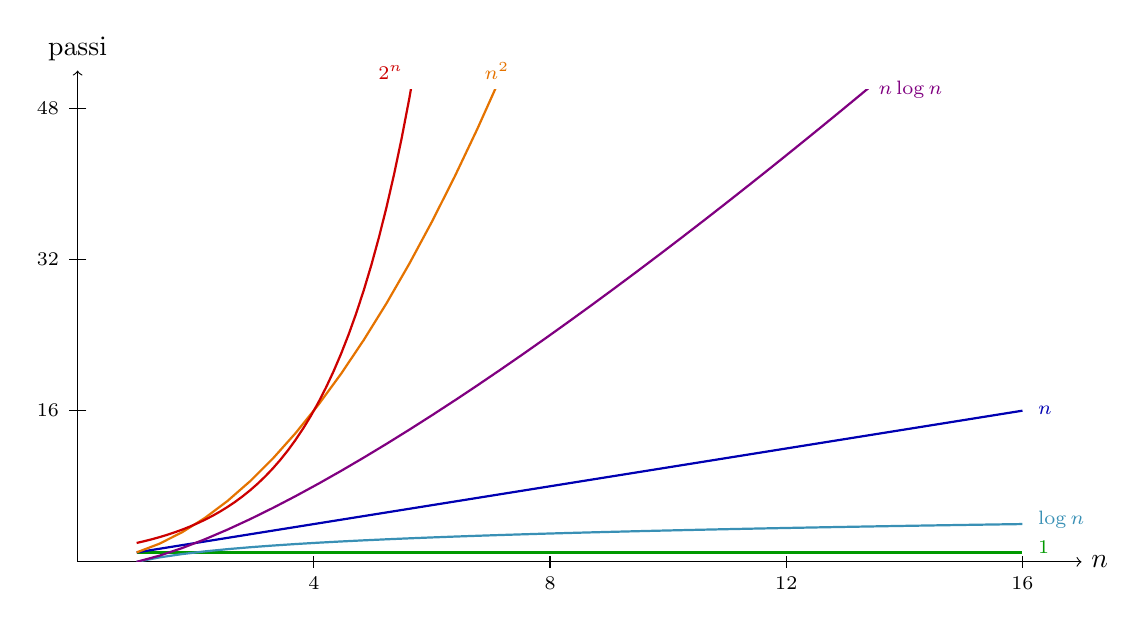
\begin{tikzpicture}[x=0.75cm,y=0.12cm]
  \draw[->] (0,0) -- (17,0) node[right] {$n$};
  \draw[->] (0,0) -- (0,52) node[above] {passi};
  \foreach \x in {4,8,12,16} \draw (\x,0.6) -- (\x,-0.6) node[below,font=\scriptsize] {\x};
  \foreach \y in {16,32,48} \draw (0.15,\y) -- (-0.15,\y) node[left,font=\scriptsize] {\y};
  \begin{scope}
    \clip (0,0) rectangle (17,50);
    \draw[thick,green!60!black] plot[domain=1:16] (\x,1);
    \draw[thick,cyan!70!black] plot[domain=1:16,samples=40] (\x,{ln(\x)/ln(2)});
    \draw[thick,blue!70!black] plot[domain=1:16] (\x,\x);
    \draw[thick,violet] plot[domain=1:16,samples=40] (\x,{\x*ln(\x)/ln(2)});
    \draw[thick,orange!90!black] plot[domain=1:16,samples=40] (\x,{\x*\x});
    \draw[thick,red!80!black] plot[domain=1:6,samples=40] (\x,{2^\x});
  \end{scope}
  \node[font=\scriptsize,text=green!60!black,anchor=west] at (16.1,1.5) {$1$};
  \node[font=\scriptsize,text=cyan!70!black,anchor=west] at (16.1,4.5) {$\log n$};
  \node[font=\scriptsize,text=blue!70!black,anchor=west] at (16.1,16) {$n$};
  \node[font=\scriptsize,text=violet,anchor=west] at (13.4,50) {$n\log n$};
  \node[font=\scriptsize,text=orange!90!black,anchor=south] at (7.1,50) {$n^2$};
  \node[font=\scriptsize,text=red!80!black,anchor=south] at (5.3,50) {$2^n$};
\end{tikzpicture}
\end{center}

\needspace{5cm}
\textbf{Dimezzare: perché $\log n$ passi.} Ricerca in un array ordinato di 16
elementi: a ogni passo resta metà dello spazio. $16 \to 8 \to 4 \to 2 \to 1$: 4 passi,
e $2^4 = 16$.
\begin{center}
\begin{tikzpicture}
  \foreach \riga/\da/\a [count=\r] in {0/0/15,1/8/15,2/8/11,3/10/11,4/10/10} {
    \foreach \i in {0,...,15} {
      \pgfmathsetmacro{\attivo}{(\i>=\da && \i<=\a) ? 1 : 0}
      \ifdim\attivo pt>0.5pt
        \node[cellina,minimum width=0.55cm,minimum height=0.5cm,fill=heapcol,font=\tiny] at (\i*0.55,-\riga*0.65) {};
      \else
        \node[cellina,minimum width=0.55cm,minimum height=0.5cm,fill=black!10!sfondo,draw=black!30,font=\tiny] at (\i*0.55,-\riga*0.65) {};
      \fi
    }
    \node[etichetta,anchor=east] at (-0.5,-\riga*0.65) {passo \riga};
  }
  \node[etichetta,anchor=west,text width=4.2cm] at (9.2,-1.3) {in arancione la parte in cui il valore può ancora trovarsi: si dimezza a ogni confronto};
\end{tikzpicture}
\end{center}

\needspace{6cm}
\textbf{Divide et impera: perché $N \log N$.} Ricorrenza $C_N = 2C_{N/2} + N$ con
$N = 8$. Ogni livello divide i pezzi a metà; a ogni livello il lavoro di
``ricombinazione'' tocca in tutto $N$ elementi. I livelli sono $\log_2 8 = 3$.
\begin{center}
\begin{tikzpicture}
  \node[cella,fill=stackcol,minimum width=6.4cm] (l0) at (0,0) {8};
  \foreach \i in {0,1} \node[cella,fill=stackcol,minimum width=3.1cm] (l1\i) at (-1.65+\i*3.3,-1) {4};
  \foreach \i in {0,...,3} \node[cella,fill=stackcol,minimum width=1.5cm] (l2\i) at (-2.4+\i*1.6,-2) {2};
  \foreach \i in {0,...,7} \node[cella,fill=stackcol,minimum width=0.7cm] (l3\i) at (-2.8+\i*0.8,-3) {1};
  \foreach \y/\t in {0/lavoro 8,-1/lavoro 4+4 = 8,-2/lavoro 2+2+2+2 = 8,-3/casi base} \node[etichetta,anchor=west] at (3.6,\y) {\t};
  \draw[decorate,decoration={brace,amplitude=5pt}] (-3.9,-3) -- (-3.9,0) node[midway,left=6pt,etichetta,text width=2cm,align=right] {$\log_2 8 = 3$ livelli};
  \node[font=\small,anchor=north] at (0,-3.6) {totale: $3$ livelli $\times$ $8$ = $N \log N$};
\end{tikzpicture}
\end{center}

% ---------------------------------------------------------------------
\section{Pattern di Codice di Laboratorio}
% ---------------------------------------------------------------------

Il ``contatore di passi'': una variabile globale \cc|passi| che ogni funzione
incrementa a ogni operazione elementare. Il \cc|main| esegue cinque funzioni di
complessità diversa per $n$ = 10, 100, 1000, 10\,000 e stampa i passi. Le funzioni
sono passate a \cc|conta| come \textbf{puntatori a funzione} (Modulo 3).

\codice{codice/m06/pattern.cpp}
\uscita{codice/m06/output/pattern.txt}

\textbf{Cosa osservare:} leggi la tabella \emph{per colonne}. Quando $n$ si
moltiplica per 10, la colonna $O(1)$ resta ferma, $O(\log n)$ cresce di 3--4,
$O(n)$ si moltiplica per 10, $O(n^2)$ per 100. Questo è tutto quello che dice la
notazione O-grande.

% ---------------------------------------------------------------------
\section{Tips \& Trappole da Esame}
% ---------------------------------------------------------------------

\begin{trappola}[: le costanti non contano]
$O(2n)$, $O(n/2)$ e $O(n + 100)$ si scrivono tutti $O(n)$. Scrivere $O(2n)$ in un
quiz non è sbagliato in senso stretto, ma mostra di non aver capito il punto.
\end{trappola}

\begin{trappola}[: annidati contro in sequenza]
Due cicli da $n$ \textbf{uno dentro l'altro} fanno $O(n^2)$; \textbf{uno dopo
l'altro} fanno $O(n) + O(n) = O(n)$. Guarda le graffe, non il numero di \cc|for|.
\end{trappola}

\begin{trappola}[: il ciclo interno non dipende sempre da n]
\cc|for (i = 0; i < n; i++) for (j = 0; j < 5; j++)| è $O(n)$: il ciclo interno fa
sempre 5 giri, è una costante. Conta i giri, non i cicli.
\end{trappola}

\begin{trappola}[: O-grande è un limite, non una misura esatta]
``L'algoritmo è $O(n^2)$'' è vero anche per un algoritmo lineare. Se il quiz chiede
quale affermazione è \emph{vera}, $O$ più grandi del necessario sono vere; se chiede
la complessità, dai la più stretta.
\end{trappola}

\begin{trappola}[: anche le chiamate costano]
Un ciclo da $n$ giri che chiama una funzione $O(n)$ a ogni giro è $O(n^2)$, anche se
vedi un solo \cc|for|. Ad esempio: chiamare una ricerca lineare dentro un ciclo.
\end{trappola}

\begin{consiglio}[: il metodo del raddoppio]
Se non sei sicuro della complessità di un pezzo di codice, aggiungi un contatore e
prova con $n$ e $2n$. Passi uguali: $O(1)$. Più uno: $O(\log n)$. Doppi: $O(n)$.
Quadruplicati: $O(n^2)$. Otto volte: $O(n^3)$.
\end{consiglio}

% ---------------------------------------------------------------------
\section{Quiz a Crocette (Prova Scritta)}
% ---------------------------------------------------------------------

\begin{quiz}{Qual è la complessità di \texttt{for (i = 0; i < n; i += 3) somma += i;}?}
  \item $O(1)$
  \item $O(\log n)$
  \item $O(n)$
  \item $O(n/3)$, diversa da $O(n)$
\end{quiz}

\begin{quiz}{Qual è la complessità di \texttt{for (i = 1; i < n; i *= 2) cont++;}?}
  \item $O(n)$
  \item $O(\log n)$
  \item $O(n^2)$
  \item $O(2^n)$
\end{quiz}

\begin{quiz}{Due cicli \texttt{for} da $n$ giri ciascuno, scritti uno \textbf{dopo} l'altro (non annidati). Complessità totale?}
  \item $O(n)$
  \item $O(n^2)$
  \item $O(2n^2)$
  \item $O(\log n)$
\end{quiz}

\begin{quiz}{$T(n) = 4n^3 + 100n^2 + 7$. Quale affermazione è \textbf{vera}?}
  \item $T(n) = O(n^2)$
  \item $T(n) = O(n^3)$
  \item $T(n) = O(100n^2)$
  \item $T(n) = O(7)$
\end{quiz}

\begin{quiz}{Se un algoritmo è $O(n^2)$, quale affermazione è sicuramente vera?}
  \item è anche $O(n^3)$
  \item è anche $O(n)$
  \item è anche $\Omega(n^2)$
  \item impiega esattamente $n^2$ passi
\end{quiz}

\begin{quiz}{Cosa significa $f(n) = \Theta(g(n))$?}
  \item $f$ cresce al più come $g$
  \item $f$ cresce almeno come $g$
  \item $f$ cresce esattamente come $g$: è sia $O(g)$ sia $\Omega(g)$
  \item $f$ e $g$ sono la stessa funzione
\end{quiz}

\begin{quiz}{Quale ordine di crescita è corretto, dal più lento al più veloce?}
  \item $\log n,\ n,\ n\log n,\ n^2,\ 2^n$
  \item $n,\ \log n,\ n^2,\ n\log n,\ 2^n$
  \item $\log n,\ n\log n,\ n,\ 2^n,\ n^2$
  \item $1,\ n,\ \log n,\ n^2,\ n\log n$
\end{quiz}

\begin{quiz}{La ricorrenza $C_N = 2C_{N/2} + N$ (divido a metà, risolvo le due metà, scorro tutto) ha soluzione:}
  \item $O(N)$
  \item $O(\log N)$
  \item $O(N \log N)$
  \item $O(N^2)$
\end{quiz}

\begin{quiz}{Un algoritmo di ordinamento per confronti ha complessità $O(n \log n)$. Sapendo che il problema è $\Omega(n \log n)$, l'algoritmo è:}
  \item ottimo
  \item migliorabile fino a $O(n)$
  \item esponenziale
  \item non si può dire nulla
\end{quiz}

\begin{quiz}{In una ricerca lineare su un array di $n$ elementi, il caso peggiore è:}
  \item l'elemento cercato è il primo
  \item l'elemento cercato è a metà
  \item l'elemento è l'ultimo o non è presente
  \item l'array è vuoto
\end{quiz}

\begin{quiz}{Qual è la complessità in \textbf{spazio} della potenza ricorsiva \texttt{pot(x, n) = x * pot(x, n-1)}?}
  \item $O(1)$, perché non usa array
  \item $O(n)$, perché le $n$ chiamate sono contemporaneamente nello stack
  \item $O(\log n)$
  \item $O(n^2)$
\end{quiz}

\begin{soluzione}[: risposte commentate]
\begin{enumerate}[label=\textbf{\arabic*.}]
  \item \textbf{C}. Circa $n/3$ giri: la costante $1/3$ si ignora. La D è il
        distrattore: $O(n/3)$ e $O(n)$ sono la stessa cosa.
  \item \textbf{B}. \cc|i| raddoppia: si arriva a $n$ in circa $\log_2 n$ passi.
  \item \textbf{A}. In sequenza si sommano: $n + n = 2n$, cioè $O(n)$.
  \item \textbf{B}. Vince il termine $n^3$. La C è uguale ad $O(n^2)$ ed è falsa.
  \item \textbf{A}. O-grande è un limite superiore: un limite più alto è ancora
        valido. Le altre non sono garantite.
  \item \textbf{C}. Definizione di $\Theta$.
  \item \textbf{A}.
  \item \textbf{C}. È la ricorrenza del MergeSort: $\log N$ livelli da $N$ di lavoro.
  \item \textbf{A}. Limite superiore dell'algoritmo e limite inferiore del problema
        coincidono.
  \item \textbf{C}. Servono $n$ confronti.
  \item \textbf{B}. Ogni chiamata occupa un record di attivazione finché le
        successive non terminano.
\end{enumerate}
\end{soluzione}

% ---------------------------------------------------------------------
\section{Laboratorio a Step (Simulazione d'Esame)}
% ---------------------------------------------------------------------

\begin{traccia}[: segmento di somma massima (dalle slide)]
Dato un array \cc|S| di $n$ interi (positivi e negativi, almeno uno positivo), un
\emph{segmento} è una sequenza di elementi \textbf{consecutivi} \cc|S[i..j]|. Si vuole
trovare il segmento con la \textbf{somma massima}; a parità di somma si preferisce il
segmento più corto. Si scriveranno tre algoritmi via via più efficienti e se ne
misurerà il costo.
\end{traccia}

\begin{step}{il contatore}
Dichiara una variabile globale \cc|long long passi| che ogni algoritmo incrementerà
a ogni somma di un elemento. Azzerala prima di ogni misura.\\[0.3em]
\textbf{Concetto nuovo:} misurare la complessità sperimentalmente.
\end{step}

\begin{step}{la soluzione ingenua}
Scrivi \cc|int sommaMassima1(const int S[], int n)|: per ogni coppia \cc|(i, j)| con
\cc|i <= j| calcola da capo la somma di \cc|S[i..j]| con un terzo ciclo. Prima di
eseguirla, prevedi la complessità.\\[0.3em]
\textbf{Concetto nuovo:} tre cicli annidati, $O(n^3)$.
\end{step}

\begin{step}{non ricalcolare}
Scrivi \cc|sommaMassima2|: osserva che la somma di \cc|S[i..j]| è la somma di
\cc|S[i..j-1]| più \cc|S[j]|, quindi non serve il terzo ciclo.\\[0.3em]
\textbf{Concetto nuovo:} riusare risultati già calcolati, da $O(n^3)$ a $O(n^2)$.
\end{step}

\begin{step}{una sola passata}
Scrivi \cc|int sommaMassima3(const int S[], int n, int& inizio, int& fine)|, che
scorre l'array \textbf{una volta} tenendo una somma ``in corso'': se diventa negativa,
la azzera e fa ripartire il segmento dall'elemento successivo (una somma negativa
può solo peggiorare quello che viene dopo). Restituisci anche gli estremi del
segmento, preferendo il più corto a parità di somma.\\[0.3em]
\textbf{Concetto nuovo:} un'idea migliore batte un computer più veloce, $O(n)$.
\end{step}

\begin{step}{il confronto}
Con \cc|srand(111222333)| genera array casuali di 10, 100 e 1000 elementi (valori
tra $-10$ e $10$) e stampa una tabella con i passi dei tre algoritmi, verificando che
diano tutti lo stesso risultato.\\[0.3em]
\textbf{Concetto nuovo:} leggere la crescita in una tabella.
\end{step}

\subsection*{Soluzione completa}
\codice{codice/m06/lab.cpp}
\uscita{codice/m06/output/lab.txt}

\begin{consiglio}[: cosa notare nella soluzione]
\begin{itemize}
  \item Da $n = 100$ a $n = 1000$ (dati $\times 10$): la versione cubica passa da
        171\,700 a 167 milioni di passi ($\times 1000$), la quadratica da 5050 a
        500\,500 ($\times 100$), la lineare da 100 a 1000 ($\times 10$).
  \item I numeri della quadratica sono esattamente $\frac{n(n+1)}{2}$ (la somma di
        Gauss), quelli della cubica circa $\frac{n^3}{6}$: le costanti cambiano, la
        crescita no.
  \item Sull'esempio piccolo il segmento migliore è \texttt{S[2..5]} =
        $3 + 5 - 2 + 4 = 10$.
\end{itemize}
\end{consiglio}

% ---------------------------------------------------------------------
\section{Domande e Risposte Modello per l'Orale}
% ---------------------------------------------------------------------

\begin{orale}[D1. Come si misura la complessità di un algoritmo?]
La si esprime in funzione della dimensione $n$ dell'input, contando il numero di
operazioni elementari eseguite (complessità temporale, nel modello RAM ogni
operazione costa 1) o il numero di celle di memoria aggiuntive (complessità
spaziale). Il costo di una sequenza è la somma dei costi; quello di un
\cc|if| è il costo della guardia più il maggiore dei due rami; quello di un ciclo è
la somma dei costi di tutte le iterazioni. Di solito si considera il caso peggiore e
si studia il comportamento asintotico, cioè come cresce il costo per $n$ grande,
ignorando costanti e termini di ordine inferiore.
\end{orale}

\begin{orale}[D2. Cosa significa O-grande?]
$f(n) = O(g(n))$ se esistono una costante $c > 0$ e un $n_0$ tali che
$f(n) \le c \cdot g(n)$ per ogni $n > n_0$. In parole: da un certo punto in poi $f$
non cresce più velocemente di $g$, a meno di una costante. È un limite superiore
asintotico; non è unico, perché anche ogni funzione più grande lo è, e per questo si
indica il più piccolo noto.
\end{orale}

\begin{orale}[D3. Differenza tra O, Omega e Theta?]
$O$ è un limite superiore: $f$ cresce al più come $g$. $\Omega$ è un limite inferiore:
$f$ cresce almeno come $g$, cioè $f(n) \ge c \cdot g(n)$ da un certo $n$ in poi.
$\Theta$ indica che valgono entrambi, quindi $f$ cresce esattamente come $g$. Per un
problema, se un algoritmo ha costo $O(f(n))$ e si dimostra che il problema richiede
$\Omega(f(n))$, l'algoritmo è ottimo e la complessità del problema è $\Theta(f(n))$:
è il caso dell'ordinamento per confronti con $n \log n$.
\end{orale}

\begin{orale}[D4. Quali sono le principali classi di complessità?]
In ordine crescente: costante $O(1)$, logaritmica $O(\log n)$, lineare $O(n)$,
$O(n \log n)$, polinomiale (quadratica $O(n^2)$, cubica $O(n^3)$, \ldots) ed
esponenziale $O(c^n)$. Un ciclo con incremento costante è lineare, uno che
moltiplica o divide per una costante è logaritmico, cicli annidati moltiplicano le
complessità. Gli algoritmi esponenziali sono impraticabili già per input piccoli.
\end{orale}

\begin{orale}[D5. Come si analizza un algoritmo ricorsivo?]
Si scrive una relazione di ricorrenza che esprime il costo per $n$ in funzione del
costo sui sottoproblemi più piccoli più il lavoro della singola chiamata. Alcune
ricorrenze fondamentali: $C_N = C_{N-1} + N$ dà $O(N^2)$; $C_N = C_{N/2} + 1$ dà
$O(\log N)$, come la ricerca binaria; $C_N = 2C_{N/2} + N$ dà $O(N \log N)$, tipica
del divide et impera come il MergeSort. Ad esempio la potenza $x^n$ calcolata come
$x \cdot x^{n-1}$ costa $O(n)$, mentre calcolata dimezzando l'esponente costa
$O(\log n)$. Nella ricorsione va considerato anche lo spazio: ogni chiamata attiva
occupa un record nello stack.
\end{orale}

% ---------------------------------------------------------------------
\section{Esercizi al PC}
% ---------------------------------------------------------------------

In ogni esercizio: \textbf{prima} scrivi su un foglio la complessità che ti
aspetti, \textbf{poi} aggiungi un contatore al codice e controlla con i numeri.

\begin{esercizio}{Un passo sì e uno no}{facile}
Conta i giri di \cc|for (i = 0; i < n; i += 2)| per $n$ = 10, 100, 1000, 10\,000 e
stampa anche \cc|passi / n|. Cosa noti nel rapporto? Che complessità è?
\end{esercizio}

\begin{esercizio}{Quadrato e triangolo}{facile}
Conta i giri di due cicli annidati completi (\cc|j| da 0 a $n$) e di due cicli ``a
triangolo'' (\cc|j| da \cc|i+1| a $n$). Stampa i rapporti con $n^2$. Hanno la stessa
complessità?
\end{esercizio}

\begin{esercizio}{Raddoppiare}{facile}
Conta i giri di \cc|for (i = 1; i < n; i *= 2)| per $n$ = 1, 10, 100, \ldots,
1\,000\,000. Di quanto crescono i passi quando $n$ si moltiplica per 10?
\end{esercizio}

\begin{esercizio}{Vince il più pesante}{facile}
Metti in sequenza un ciclo da $n$ giri e due cicli annidati da $n$. Stampa i passi
dei due blocchi e la percentuale di lavoro del secondo per $n$ = 10, 100, 1000.
\end{esercizio}

\begin{esercizio}{I tre casi della ricerca lineare}{medio}
Su un array di 1000 elementi, conta i confronti della ricerca lineare nel caso
migliore, nel caso peggiore (ultimo elemento e assente) e nel caso medio (media
cercando, uno alla volta, tutti gli elementi presenti).
\end{esercizio}

\begin{esercizio}{L'esempio delle slide}{medio}
Implementa la funzione \cc|func(n)| delle slide (ciclo esterno da $n/2$ a $n$, due
cicli interni che raddoppiano) e verifica che \cc|count| sia esattamente
$(n/2 + 1) \cdot L \cdot L$, dove $L$ è il numero di giri di un ciclo che raddoppia
fino a $n$. Che complessità ne deduci?
\end{esercizio}

\begin{esercizio}{Potenza lenta e veloce}{medio}
Implementa le due versioni ricorsive della potenza delle slide e conta le
moltiplicazioni per $2^{10}$, $2^{30}$, $2^{62}$ (usa \cc|long long|).
\end{esercizio}

\begin{esercizio}{Numeri primi}{medio}
Scrivi due test di primalità: uno che prova tutti i divisori da 2 a $n-1$ e uno che si
ferma quando \cc|d * d > n|. Conta le divisioni sui numeri primi 97, 9973 e 999\,983 e
spiega perché basta arrivare alla radice quadrata.
\end{esercizio}

\begin{esercizio}{Lineare contro binaria}{difficile}
Su array ordinati di $10^3$, $10^5$ e $10^6$ elementi (allocati con \cc|new|), conta
i confronti della ricerca lineare e della ricerca binaria cercando un valore assente.
\end{esercizio}

\begin{esercizio}{Fibonacci}{difficile}
Scrivi Fibonacci ricorsivo ``ingenuo'' e iterativo e confronta il numero di chiamate
ricorsive con il numero di giri del ciclo per $n$ = 10, 15, \ldots, 35. Di quanto si
moltiplicano le chiamate a ogni $+5$?
\end{esercizio}

\subsection*{Soluzioni}
Le soluzioni commentate, con il codice e l'output reale, sono nel PDF separato
\textbf{Soluzioni} (\texttt{soluzioni-light.pdf} / \texttt{soluzioni-dark.pdf}),
allo stesso numero di esercizio. Il codice è anche in \texttt{codice/m06/}.

% =====================================================================
\chapter{Modulo 7 -- Algoritmi di Ordinamento e Ricerca}
% =====================================================================

% ---------------------------------------------------------------------
\section{Teoria \& Analogia Chiave}
% ---------------------------------------------------------------------

\subsection*{Perché ordinare}

Ordinare un array significa disporre i suoi elementi in ordine crescente (o
decrescente). Sembra un problema banale, ma è uno dei più studiati
dell'informatica, per due motivi:
\begin{itemize}
  \item i dati ordinati si \textbf{cercano} enormemente più in fretta: la ricerca
        binaria su un milione di elementi ordinati richiede 20 confronti, quella
        lineare un milione (Esercizio~6.9);
  \item molti altri problemi diventano facili sui dati ordinati: trovare i
        duplicati, il mediano, gli elementi comuni a due elenchi (Esercizio~7.10).
\end{itemize}
In questo modulo vediamo cinque algoritmi di ordinamento: tre semplici e lenti
($O(n^2)$) e due ``intelligenti'' e veloci ($O(n \log n)$), basati sul divide et
impera del Modulo 6. Per ognuno devi sapere: \textbf{l'idea}, \textbf{il codice}
e \textbf{la complessità}.

Due proprietà che compaiono nei quiz:
\begin{itemize}
  \item un algoritmo è \textbf{stabile} se due elementi con la stessa chiave
        restano nell'ordine in cui erano. Esempio: ordino per voto degli studenti
        già in ordine alfabetico; con un algoritmo stabile, a parità di voto restano
        in ordine alfabetico (Esercizio~7.6);
  \item un algoritmo è \textbf{in loco} (\emph{in place}) se usa solo una quantità
        costante di memoria in più oltre all'array.
\end{itemize}

\subsection*{Bubble sort (ordinamento a bolle)}

\textbf{Idea.} Scorri l'array confrontando gli elementi \emph{vicini}, \cc|a[j]| e
\cc|a[j+1]|: se sono nell'ordine sbagliato li scambi. Alla fine della prima passata
l'elemento più grande è ``salito'' fino in fondo, come una bolla nell'acqua. Ripeti:
la seconda passata porta in fondo il secondo più grande, e così via. Dopo $n-1$
passate l'array è ordinato.

\begin{lstlisting}
for (int i = 0; i < n - 1; i++) {            // n-1 passate
    bool scambiato = false;
    for (int j = 0; j < n - 1 - i; j++)      // gli ultimi i sono già a posto
        if (a[j] > a[j + 1]) { scambia(a[j], a[j + 1]); scambiato = true; }
    if (!scambiato) break;                   // nessuno scambio: già ordinato
}
\end{lstlisting}

\textbf{Complessità.} Due cicli annidati ``a triangolo'': circa $n^2/2$ confronti,
quindi $O(n^2)$ nel caso peggiore (array al contrario) e medio. Con il controllo
\cc|scambiato|, se l'array è già ordinato basta una passata: caso migliore $O(n)$.
Stabile e in loco.

\subsection*{Selection sort (ordinamento per selezione)}

\textbf{Idea.} Cerca il \textbf{minimo} di tutto l'array e scambialo con il primo
elemento. Poi cerca il minimo tra gli elementi dal secondo in poi e mettilo in
seconda posizione. E così via: alla passata $i$ selezioni il minimo della parte
non ancora ordinata e lo metti in posizione $i$.

\begin{lstlisting}
for (int i = 0; i < n - 1; i++) {
    int iMin = i;
    for (int j = i + 1; j < n; j++)
        if (a[j] < a[iMin]) iMin = j;
    scambia(a[i], a[iMin]);
}
\end{lstlisting}

\textbf{Complessità.} I confronti sono sempre $n(n-1)/2$, \emph{qualunque} sia
l'input: $O(n^2)$ in tutti i casi, anche se l'array è già ordinato. Fa però
pochissimi scambi (al più $n-1$). In loco, non stabile nella versione con scambi.

\subsection*{Insertion sort (ordinamento per inserimento)}

\begin{analogia}[: le carte in mano]
È il modo in cui ordini le carte da gioco: le prendi una alla volta e
\textbf{inserisci} ognuna al posto giusto tra quelle che hai già in mano, facendo
scorrere a destra quelle più grandi.
\end{analogia}

\begin{lstlisting}
for (int i = 1; i < n; i++) {
    int x = a[i];                  // la carta da inserire
    int j = i - 1;
    while (j >= 0 && a[j] > x) {   // sposto a destra le carte più grandi
        a[j + 1] = a[j];
        j--;
    }
    a[j + 1] = x;                  // la metto nel buco rimasto
}
\end{lstlisting}

\textbf{Complessità.} Caso peggiore (array al contrario): ogni elemento attraversa
tutti i precedenti, $O(n^2)$. Caso migliore (già ordinato): il \cc|while| non parte
mai, $O(n)$. Su array \emph{quasi} ordinati è molto veloce. Stabile e in loco. Tra i
tre algoritmi semplici è il migliore nella pratica (nel laboratorio fa circa metà
dei confronti del bubble sort).

\subsection*{Merge sort (ordinamento per fusione)}

È il primo algoritmo \textbf{divide et impera}, ed è \textbf{ricorsivo} (la
ricorsione si approfondisce nel Modulo 8).
\begin{passopasso}[: merge sort]
\begin{enumerate}
  \item \textbf{Dividi}: taglia l'array a metà.
  \item \textbf{Conquista}: ordina ricorsivamente la metà sinistra e la metà destra.
        Il caso base è un pezzo con 0 o 1 elementi, che è già ordinato.
  \item \textbf{Combina}: \textbf{fondi} (\emph{merge}) le due metà ordinate in un
        unico array ordinato.
\end{enumerate}
\end{passopasso}

Il cuore è la \textbf{fusione}. Hai due mazzetti di carte già ordinati, a faccia in
su: guardi le due carte in cima, prendi la più piccola e la metti nel mazzo
risultato. Ripeti finché uno dei due mazzetti finisce, poi accodi il resto
dell'altro. Ogni carta viene toccata una volta: fondere costa $O(n)$. Serve però un
\textbf{array di appoggio} dove scrivere il risultato: il merge sort \textbf{non} è
in loco.

\begin{lstlisting}
void merge(int a[], int sx, int centro, int dx) {
    int* b = new int[dx - sx + 1];          // appoggio
    int i = sx, j = centro + 1, k = 0;
    while (i <= centro && j <= dx)          // finché entrambe le metà hanno elementi
        b[k++] = (a[i] <= a[j]) ? a[i++] : a[j++];
    while (i <= centro) b[k++] = a[i++];    // avanzi della sinistra
    while (j <= dx) b[k++] = a[j++];        // avanzi della destra
    for (k = 0; k < dx - sx + 1; k++) a[sx + k] = b[k];
    delete[] b;
}
void mergeSort(int a[], int sx, int dx) {
    if (sx >= dx) return;                   // caso base
    int centro = (sx + dx) / 2;
    mergeSort(a, sx, centro);
    mergeSort(a, centro + 1, dx);
    merge(a, sx, centro, dx);
}
\end{lstlisting}

\textbf{Complessità.} È la ricorrenza $C_N = 2C_{N/2} + N$ del Modulo 6: $\log n$
livelli di dimezzamento, lavoro $n$ per livello, quindi $O(n \log n)$ \textbf{in
tutti i casi} (migliore, medio e peggiore), perché divide sempre a metà
indipendentemente dai dati. Spazio $O(n)$ per l'appoggio. È \textbf{stabile} grazie
al \cc|<=| nella fusione: a parità prende prima l'elemento di sinistra.

\subsection*{Quick sort (ordinamento rapido)}

\begin{passopasso}[: quick sort]
\begin{enumerate}
  \item Scegli un elemento, il \textbf{pivot} (perno). Nella versione delle slide è
        l'elemento centrale.
  \item \textbf{Partiziona}: sposta a sinistra tutti gli elementi minori del pivot e a
        destra tutti quelli maggiori. Ora ogni elemento della parte sinistra è
        $\le$ di ogni elemento della parte destra.
  \item Ordina ricorsivamente la parte sinistra e la parte destra. Non serve nessuna
        fusione: le due parti sono già ``in ordine tra loro''.
\end{enumerate}
\end{passopasso}

La partizione delle slide usa due indici che si vengono incontro: \cc|i| parte da
sinistra e avanza finché trova un elemento che \emph{non} è minore del pivot (sta
dalla parte sbagliata); \cc|j| parte da destra e arretra finché trova un elemento che
non è maggiore del pivot. Quando entrambi si fermano, scambi \cc|a[i]| e \cc|a[j]|
e prosegui. Quando \cc|i| supera \cc|j| la partizione è finita.

\begin{lstlisting}
void quickSort(int a[], int sx, int dx) {
    int i = sx, j = dx;
    int pivot = a[(sx + dx) / 2];
    while (i <= j) {
        while (a[i] < pivot) i++;
        while (a[j] > pivot) j--;
        if (i <= j) { scambia(a[i], a[j]); i++; j--; }
    }
    if (sx < j) quickSort(a, sx, j);    // ci sono ancora elementi a sinistra
    if (i < dx) quickSort(a, i, dx);    // ci sono ancora elementi a destra
}
\end{lstlisting}

\textbf{Complessità.} Dipende da quanto bene il pivot divide l'array:
\begin{itemize}
  \item \textbf{caso migliore e medio}: il pivot divide in due parti più o meno
        uguali, quindi $\log n$ livelli da $n$: $O(n \log n)$. Le slide precisano
        che basta una divisione ``proporzionale'' (anche 10\%--90\%) perché resti
        $O(n \log n)$;
  \item \textbf{caso peggiore}: il pivot è sempre il minimo o il massimo, le parti
        hanno $0$ e $n-1$ elementi e i livelli diventano $n$: $O(n^2)$. Succede ad
        esempio scegliendo come pivot il \emph{primo} elemento di un array già
        ordinato (Esercizio~7.7: 1\,999\,000 confronti contro 20\,010).
\end{itemize}
In pratica è il più veloce di tutti (nel laboratorio batte il merge sort in tempo),
perché lavora in loco e fa operazioni semplici. Non è stabile.

\subsection*{Riepilogo da memorizzare}

\begin{center}\small
\begin{tabular}{lllllcc}
\toprule
\textbf{Algoritmo} & \textbf{Migliore} & \textbf{Medio} & \textbf{Peggiore} & \textbf{Spazio extra} & \textbf{Stabile} & \textbf{In loco} \\
\midrule
Bubble    & $O(n)$       & $O(n^2)$      & $O(n^2)$      & $O(1)$      & sì & sì \\
Selection & $O(n^2)$     & $O(n^2)$      & $O(n^2)$      & $O(1)$      & no & sì \\
Insertion & $O(n)$       & $O(n^2)$      & $O(n^2)$      & $O(1)$      & sì & sì \\
Merge     & $O(n\log n)$ & $O(n\log n)$  & $O(n\log n)$  & $O(n)$      & sì & no \\
Quick     & $O(n\log n)$ & $O(n\log n)$  & $O(n^2)$      & $O(\log n)$ (stack) & no & sì \\
\bottomrule
\end{tabular}
\end{center}
Ricorda dal Modulo 6 che \textbf{nessun} algoritmo che ordina confrontando gli
elementi può fare meglio di $\Omega(n \log n)$ nel caso peggiore: merge sort è
quindi \textbf{ottimo}. Si può fare meglio solo \emph{senza} confronti, quando si
sa qualcosa sui valori: ad esempio il counting sort per valori interi in un
intervallo piccolo, come i voti da 18 a 30 (Esercizio~7.8).

\subsection*{Ricerca lineare e ricerca binaria}

\textbf{Ricerca lineare}: controlla gli elementi uno a uno. Funziona su qualunque
array, ordinato o no. Costo $O(n)$ nel caso peggiore e medio.

\textbf{Ricerca binaria} (o dicotomica): funziona \textbf{solo su array
ordinati}. Guarda l'elemento centrale: se è quello cercato hai finito; se è più
piccolo, il valore può stare solo nella metà destra; se è più grande, solo nella metà
sinistra. Butti via metà dell'array e ripeti. È la rubrica del Modulo 6: $O(\log n)$.

\begin{lstlisting}
int ricercaBinaria(const int a[], int n, int x) {
    int sx = 0, dx = n - 1;
    while (sx <= dx) {                   // finché l'intervallo non è vuoto
        int m = (sx + dx) / 2;
        if (a[m] == x) return m;
        if (a[m] < x) sx = m + 1;        // butto la metà sinistra (m compreso)
        else dx = m - 1;                 // butto la metà destra (m compreso)
    }
    return -1;                           // non trovato
}
\end{lstlisting}
Se devi cercare \emph{molte} volte nello stesso array, conviene ordinarlo una volta
($O(n \log n)$) e poi fare tante ricerche binarie ($O(\log n)$ ciascuna).

\begin{inparole}
\begin{itemize}
  \item Bubble: scambi tra vicini, il massimo ``sale'' in fondo. Selection: scegli il
        minimo e mettilo davanti. Insertion: inserisci come le carte.
        Tutti $O(n^2)$.
  \item Merge: dividi a metà, ordina le metà, fondi. Sempre $O(n \log n)$, serve un
        array d'appoggio, stabile.
  \item Quick: pivot, partiziona, ricorri. $O(n \log n)$ in media, $O(n^2)$ con pivot
        sfortunati, in loco, il più veloce in pratica.
  \item Ricerca binaria: solo su array ordinati, dimezza a ogni passo, $O(\log n)$.
\end{itemize}
\end{inparole}

% ---------------------------------------------------------------------
\section{Rappresentazione Visiva della Memoria (TikZ)}
% ---------------------------------------------------------------------

\textbf{Bubble sort: la prima passata.} In giallo la coppia confrontata; il
massimo (82) arriva in fondo.
\begin{center}
\begin{tikzpicture}
  \foreach \riga/\vals/\hl in {0/{38,27,43,3,9,82,10}/0, 1/{27,38,43,3,9,82,10}/2, 2/{27,38,3,43,9,82,10}/3, 3/{27,38,3,9,43,82,10}/4, 4/{27,38,3,9,43,10,82}/9} {
    \foreach \v [count=\i from 0] in \vals {
      \pgfmathsetmacro{\evid}{(\i==\hl || \i==\hl+1) ? 1 : 0}
      \ifdim\evid pt>0.5pt
        \node[cellina,fill=yellow!40!sfondo] at (\i*0.8,-\riga*0.7) {\v};
      \else
        \node[cellina,fill=sfondo] at (\i*0.8,-\riga*0.7) {\v};
      \fi
    }
  }
  \node[etichetta,anchor=west,text width=5cm] at (6,-1.4) {si confrontano coppie vicine e si scambiano se fuori ordine; righe intermedie omesse};
  \node[cellina,fill=green!25!sfondo] at (4.8,-2.8) {82};
\end{tikzpicture}
\end{center}

\needspace{7cm}
\textbf{Merge sort sull'esempio delle slide.} In alto le divisioni, in basso le
fusioni.
\begin{center}
\begin{tikzpicture}[blocco/.style={draw,fill=stackcol,font=\ttfamily\footnotesize,minimum height=0.55cm,inner sep=2pt}]
  \node[blocco] (a) at (0,0) {38 27 43 3 9 82 10};
  \node[blocco] (b1) at (-2.4,-0.9) {38 27 43 3};
  \node[blocco] (b2) at (2.4,-0.9) {9 82 10};
  \node[blocco] (c1) at (-3.4,-1.8) {38 27};
  \node[blocco] (c2) at (-1.4,-1.8) {43 3};
  \node[blocco] (c3) at (1.6,-1.8) {9 82};
  \node[blocco] (c4) at (3.4,-1.8) {10};
  \foreach \x/\v [count=\i] in {-3.9/38,-2.9/27,-1.9/43,-0.9/3,1.1/9,2.1/82}
    \node[blocco] (d\i) at (\x,-2.7) {\v};
  \draw (a) -- (b1); \draw (a) -- (b2);
  \draw (b1) -- (c1); \draw (b1) -- (c2); \draw (b2) -- (c3); \draw (b2) -- (c4);
  \draw (c1) -- (d1); \draw (c1) -- (d2); \draw (c2) -- (d3); \draw (c2) -- (d4); \draw (c3) -- (d5); \draw (c3) -- (d6);
  \node[blocco,fill=heapcol] (e1) at (-3.4,-3.7) {27 38};
  \node[blocco,fill=heapcol] (e2) at (-1.4,-3.7) {3 43};
  \node[blocco,fill=heapcol] (e3) at (1.6,-3.7) {9 82};
  \node[blocco,fill=heapcol] (e4) at (3.4,-3.7) {10};
  \node[blocco,fill=heapcol] (f1) at (-2.4,-4.6) {3 27 38 43};
  \node[blocco,fill=heapcol] (f2) at (2.4,-4.6) {9 10 82};
  \node[blocco,fill=green!20!sfondo] (g) at (0,-5.5) {3 9 10 27 38 43 82};
  \draw (d1) -- (e1); \draw (d2) -- (e1); \draw (d3) -- (e2); \draw (d4) -- (e2); \draw (d5) -- (e3); \draw (d6) -- (e3); \draw (c4) -- (e4);
  \draw (e1) -- (f1); \draw (e2) -- (f1); \draw (e3) -- (f2); \draw (e4) -- (f2);
  \draw (f1) -- (g); \draw (f2) -- (g);
  \node[etichetta,anchor=west] at (4.6,-1.3) {DIVIDI};
  \node[etichetta,anchor=west] at (4.6,-4.6) {FONDI (merge)};
\end{tikzpicture}
\end{center}

\needspace{5cm}
\textbf{Quick sort: una partizione.} Pivot = elemento centrale (3). \cc|i| avanza
finché \cc|a[i] < 3|, \cc|j| arretra finché \cc|a[j] > 3|; poi si scambia.
\begin{center}
\begin{tikzpicture}
  \foreach \v [count=\i from 0] in {38,27,43,3,9,82,10}
    \node[cellina,fill=sfondo] (q\i) at (\i*0.8,0) {\v};
  \node[cellina,fill=yellow!40!sfondo] at (q3) {3};   % il pivot evidenziato
  \draw[freccia] ($(q0.south)+(0,-0.5)$) node[below,font=\small] {i} -- (q0.south);
  \draw[freccia] ($(q3.south)+(0,-0.5)$) node[below,font=\small] {j} -- (q3.south);
  \node[etichetta,anchor=west,text width=7.6cm] at (6,0) {
    \texttt{a[0] = 38} non è $< 3$: \texttt{i} si ferma subito. \texttt{j} arretra da 10
    fino a \texttt{a[3] = 3}, che non è $> 3$. Si scambiano: \texttt{3 27 43 38 9 82 10}.
    Alla fine a sinistra c'è solo \texttt{3}, a destra tutto il resto: si ricorre sulla destra.};
\end{tikzpicture}
\end{center}

% ---------------------------------------------------------------------
\section{Pattern di Codice di Laboratorio}
% ---------------------------------------------------------------------

I cinque algoritmi e la ricerca binaria, scritti nella forma più compatta e
leggibile, provati sullo stesso array delle slide (con un 27 doppio, per verificare
i duplicati). I tre algoritmi semplici hanno la stessa firma e sono chiamati tramite
un array di puntatori a funzione.

\codice{codice/m07/pattern.cpp}
\uscita{codice/m07/output/pattern.txt}

% ---------------------------------------------------------------------
\section{Tips \& Trappole da Esame}
% ---------------------------------------------------------------------

\begin{trappola}[: ricerca binaria su array non ordinato]
Compila e gira, ma dà risultati sbagliati senza nessun errore. La ricerca binaria
richiede che l'array sia \textbf{ordinato}: se non lo è, ordinalo prima.
\end{trappola}

\begin{trappola}[: indici fuori di uno]
I bug più comuni: \cc|j < n - i| invece di \cc|j < n - 1 - i| nel bubble sort (si
legge \cc|a[n]|), \cc|while (sx < dx)| invece di \cc|<=| nella ricerca binaria (salta
l'ultimo elemento), \cc|mergeSort(a, 0, n)| invece di \cc|n - 1|. Prova sempre con
array di 0, 1 e 2 elementi.
\end{trappola}

\begin{trappola}[: l'array d'appoggio del merge]
Un array locale \cc|int b[n];| con \cc|n| variabile non è C++ standard (alcuni
compilatori lo accettano) e con $n$ grande esaurisce lo stack. Usa \cc|new int[...]|
e \cc|delete[]|, oppure allocalo una volta sola e passalo alle chiamate (come nel
laboratorio).
\end{trappola}

\begin{trappola}[: complessità ``tutti i casi'']
Domande tipiche: il merge sort è $O(n \log n)$ \textbf{anche} nel caso peggiore; il
quick sort no ($O(n^2)$). Il selection sort è $O(n^2)$ \textbf{anche} nel caso
migliore; bubble (con il flag) e insertion no ($O(n)$).
\end{trappola}

\begin{consiglio}[: overload con l'involucro]
Merge sort e quick sort lavorano su \cc|(a, sx, dx)|. Scrivi anche una versione
\cc|ordina(int a[], int n)| che chiama \cc|mergeSort(a, 0, n - 1)|: così chi usa la
funzione non deve preoccuparsi degli indici.
\end{consiglio}

\begin{consiglio}[: l'operatore virgola]
Nel laboratorio \cc|while (j >= 0 && (confronti++, a[j] > x))| usa l'operatore
virgola: esegue \cc|confronti++| e poi vale \cc|a[j] > x|. Serve solo a contare i
confronti senza cambiare l'algoritmo; nel codice d'esame non serve.
\end{consiglio}

% ---------------------------------------------------------------------
\section{Quiz a Crocette (Prova Scritta)}
% ---------------------------------------------------------------------

\begin{quiz}{Qual è la complessità del merge sort nel caso peggiore?}
  \item $O(n)$
  \item $O(n \log n)$
  \item $O(n^2)$
  \item $O(\log n)$
\end{quiz}

\begin{quiz}{Qual è la complessità del quick sort nel caso peggiore?}
  \item $O(n \log n)$
  \item $O(n)$
  \item $O(n^2)$
  \item $O(2^n)$
\end{quiz}

\begin{quiz}{Quale algoritmo esegue sempre lo stesso numero di confronti, anche se l'array è già ordinato?}
  \item bubble sort con controllo sugli scambi
  \item insertion sort
  \item selection sort
  \item nessuno
\end{quiz}

\begin{quiz}{Cosa richiede la ricerca binaria per funzionare correttamente?}
  \item un array di numeri interi
  \item un array ordinato
  \item un array di dimensione pari
  \item un array senza duplicati
\end{quiz}

\begin{quiz}{Quale affermazione sul merge sort è \textbf{falsa}?}
  \item segue il paradigma divide et impera
  \item è stabile
  \item ordina in loco senza memoria aggiuntiva
  \item la fusione di due metà ordinate costa tempo lineare
\end{quiz}

\begin{quiz}{Nel quick sort, cosa garantisce la fase di partizione?}
  \item che le due parti abbiano la stessa dimensione
  \item che ogni elemento della parte sinistra sia $\le$ di ogni elemento della parte destra
  \item che la parte sinistra sia già ordinata
  \item che il pivot sia il mediano
\end{quiz}

\begin{quiz}{Un algoritmo di ordinamento si dice stabile se:}
  \item non va mai in crash
  \item ha la stessa complessità in tutti i casi
  \item mantiene l'ordine relativo degli elementi con chiave uguale
  \item non usa memoria aggiuntiva
\end{quiz}

\begin{quiz}{Quanti confronti servono al più per trovare un elemento con la ricerca binaria in un array ordinato di 1000 elementi?}
  \item circa 10
  \item circa 100
  \item circa 500
  \item 1000
\end{quiz}

\begin{quiz}{Quale algoritmo ha complessità $O(n)$ nel caso migliore (array già ordinato)?}
  \item merge sort
  \item selection sort
  \item insertion sort
  \item quick sort
\end{quiz}

\begin{quiz}{Si può ordinare per confronti con complessità $O(n)$ nel caso peggiore?}
  \item sì, con il quick sort
  \item sì, con il bubble sort ottimizzato
  \item no: ogni ordinamento per confronti è $\Omega(n \log n)$ nel caso peggiore
  \item no, il limite è $\Omega(n^2)$
\end{quiz}

\begin{soluzione}[: risposte commentate]
\begin{enumerate}[label=\textbf{\arabic*.}]
  \item \textbf{B}. Divide sempre a metà: $O(n \log n)$ in ogni caso.
  \item \textbf{C}. Con pivot sempre estremo le partizioni sono sbilanciate.
  \item \textbf{C}. Cerca comunque il minimo in tutta la parte restante.
  \item \textbf{B}. I duplicati (D) non sono un problema.
  \item \textbf{C}. Serve un array d'appoggio di dimensione $n$.
  \item \textbf{B}. Le dimensioni possono essere molto diverse (A falsa); le due
        parti vanno poi ordinate ricorsivamente (C falsa).
  \item \textbf{C}.
  \item \textbf{A}. $2^{10} = 1024$: circa 10 dimezzamenti.
  \item \textbf{C}. Il \cc|while| interno non parte mai: un confronto per elemento.
        Vale anche per il bubble sort con il flag, che però non è tra le risposte.
  \item \textbf{C}. Limite inferiore del problema (Modulo 6). Il counting sort è
        lineare perché \emph{non} confronta.
\end{enumerate}
\end{soluzione}

% ---------------------------------------------------------------------
\section{Laboratorio a Step (Simulazione d'Esame)}
% ---------------------------------------------------------------------

\begin{traccia}[: prestazioni degli algoritmi di ordinamento (dalle slide)]
Implementare un metodo \cc|generaArrayCasuale(int* a, int num)| e gli algoritmi
di ordinamento; generare array di dimensioni crescenti per potenze di 10 e
confrontare le prestazioni degli algoritmi al crescere della dimensione, misurando
il tempo con \cc|<chrono>| come indicato nelle slide.
\end{traccia}

\begin{step}{gli strumenti}
Scrivi \cc|generaArrayCasuale|, \cc|copia| (per ordinare ogni volta la
\emph{stessa} sequenza) e \cc|bool ordinato(const int* a, int n)| per verificare il
risultato. Dichiara un contatore globale di confronti.\\[0.3em]
\textbf{Concetto nuovo:} misurare in modo equo (stessi dati per tutti).
\end{step}

\begin{step}{due algoritmi quadratici}
Implementa bubble sort (con uscita anticipata) e insertion sort, incrementando il
contatore a ogni confronto tra elementi.\\[0.3em]
\textbf{Concetto nuovo:} algoritmi $O(n^2)$.
\end{step}

\begin{step}{merge sort}
Implementa il merge sort allocando l'array d'appoggio \textbf{una sola volta} in una
funzione involucro \cc|mergeSort(int a[], int n)| e passandolo alle chiamate
ricorsive.\\[0.3em]
\textbf{Concetto nuovo:} divide et impera, fusione, memoria aggiuntiva $O(n)$.
\end{step}

\begin{step}{quick sort}
Implementa il quick sort con pivot centrale e partizione a due indici, come nelle
slide, più l'involucro \cc|quickSort(int a[], int n)|.\\[0.3em]
\textbf{Concetto nuovo:} partizione, ordinamento in loco.
\end{step}

\begin{step}{il confronto}
Scrivi \cc|misura(nome, puntatoreAFunzione, array, n)|, che copia l'array, azzera
il contatore, cronometra l'ordinamento con \cc|high_resolution_clock| e stampa
confronti e millisecondi. Usala per $n$ = $10^2$, $10^3$, $10^4$, $10^5$ (i quadratici
solo fino a $10^4$).\\[0.3em]
\textbf{Concetto nuovo:} misurare i tempi reali; puntatori a funzione come parametri.
\end{step}

\subsection*{Soluzione completa}
\codice{codice/m07/lab.cpp}
\uscita{codice/m07/output/lab.txt}

\begin{consiglio}[: cosa notare nella soluzione]
\begin{itemize}
  \item I \textbf{tempi} cambiano a ogni esecuzione e da PC a PC; i
        \textbf{confronti} no. Per questo il contatore è più affidabile per studiare la
        complessità.
  \item Da $n = 1000$ a $n = 10\,000$ il bubble sort passa da circa 0{,}5 a 50 milioni
        di confronti ($\times 100$): quadratico. Merge e quick crescono di poco più di
        $\times 10$: $n \log n$.
  \item Il quick sort fa \emph{più} confronti del merge sort ma impiega \emph{meno}
        tempo: non copia avanti e indietro in un array d'appoggio.
  \item \cc|setw(10)| (da \cc|<iomanip>|) stampa il numero in una colonna larga 10
        caratteri, così la tabella resta allineata.
\end{itemize}
\end{consiglio}

% ---------------------------------------------------------------------
\section{Domande e Risposte Modello per l'Orale}
% ---------------------------------------------------------------------

\begin{orale}[D1. Come funziona il merge sort e qual è la sua complessità?]
È un algoritmo divide et impera: divide l'array in due metà, le ordina
ricorsivamente fino ad arrivare a sottoarray di un elemento (caso base) e poi le
fonde con la procedura merge, che scorre le due metà ordinate e prende ogni volta il
minore dei due elementi in testa. La fusione costa $O(n)$ e i livelli di ricorsione
sono $\log n$, perciò la complessità è $O(n \log n)$ nel caso migliore, medio e
peggiore. Richiede un array d'appoggio, quindi spazio $O(n)$, ed è stabile.
\end{orale}

\begin{orale}[D2. Come funziona il quick sort? Qual è il suo caso peggiore?]
Si sceglie un pivot e si partiziona l'array in modo che a sinistra ci siano gli
elementi minori o uguali al pivot e a destra quelli maggiori o uguali; poi si
ordinano ricorsivamente le due parti, senza bisogno di fusione. Se le partizioni sono
bilanciate (anche solo in proporzione costante) la complessità è $O(n \log n)$, che è
anche il caso medio. Il caso peggiore si ha quando il pivot è sempre il minimo o il
massimo: le partizioni hanno dimensione $0$ e $n-1$ e la complessità diventa
$O(n^2)$, ad esempio con pivot sul primo elemento di un array già ordinato. Ordina in
loco e in pratica è il più veloce.
\end{orale}

\begin{orale}[D3. Differenza tra bubble, selection e insertion sort?]
Sono tutti $O(n^2)$ nel caso peggiore. Il bubble sort scambia elementi adiacenti
fuori ordine, portando a ogni passata il massimo in fondo; con il controllo sugli
scambi termina in $O(n)$ se l'array è ordinato. Il selection sort cerca a ogni
passata il minimo della parte non ordinata e lo mette in posizione: fa sempre
$n(n-1)/2$ confronti ma pochi scambi. L'insertion sort inserisce ogni elemento al suo
posto tra i precedenti già ordinati: $O(n)$ nel caso migliore ed efficiente su array
quasi ordinati. Bubble e insertion sono stabili.
\end{orale}

\begin{orale}[D4. Come funziona la ricerca binaria e perché è logaritmica?]
Si applica a un array ordinato. Si confronta il valore cercato con l'elemento
centrale: se coincide si è trovato; se è maggiore si prosegue nella metà destra,
altrimenti nella sinistra. A ogni passo l'intervallo di ricerca si dimezza, quindi
dopo al più circa $\log_2 n$ confronti l'intervallo diventa vuoto. La ricorrenza è
$C_N = C_{N/2} + 1$, con soluzione $O(\log n)$.
\end{orale}

\begin{orale}[D5. Cosa significa che un ordinamento è stabile? E in loco?]
È stabile se elementi con la stessa chiave mantengono, dopo l'ordinamento, l'ordine
relativo che avevano prima: ad esempio studenti già in ordine alfabetico, ordinati
per voto, restano in ordine alfabetico a parità di voto. Merge, insertion e bubble
sort sono stabili; selection e quick sort no. È in loco se usa solo memoria
aggiuntiva costante (o al più lo stack della ricorsione): tutti tranne il merge sort,
che ha bisogno di un array d'appoggio.
\end{orale}

% ---------------------------------------------------------------------
\section{Esercizi al PC}
% ---------------------------------------------------------------------

\begin{esercizio}{Bubble sort e passate}{facile}
Modifica il bubble sort con uscita anticipata in modo che restituisca il numero di
passate eseguite. Provalo su un array già ordinato, su uno quasi ordinato (due
elementi scambiati) e su uno al contrario.
\end{esercizio}

\begin{esercizio}{Selection sort decrescente}{facile}
Scrivi un selection sort che ordina in modo \textbf{decrescente} (cerca il massimo)
e stampa l'array dopo ogni passata.
\end{esercizio}

\begin{esercizio}{Insertion sort di stringhe}{facile}
Ordina in ordine alfabetico un array di \cc|string| con l'insertion sort. Inserisci
anche un nome che inizia con la minuscola: dove finisce, e perché?
\end{esercizio}

\begin{esercizio}{Ricerca binaria al rallentatore}{facile}
Scrivi la ricerca binaria iterativa stampando a ogni passo \cc|sx|, \cc|dx|, \cc|m| e
\cc|a[m]|. Cerca un valore presente e uno assente.
\end{esercizio}

\begin{esercizio}{Ricerca binaria ricorsiva}{medio}
Scrivi la ricerca binaria in versione ricorsiva e una funzione
\cc|posizioneInserimento(a, n, x)| che restituisce la prima posizione in cui
\cc|x| si può inserire mantenendo l'ordine (con duplicati: la prima occorrenza).
\end{esercizio}

\begin{esercizio}{Merge sort stabile di studenti}{medio}
Ordina per voto con il merge sort un array di \cc|struct Studente| (nome, voto) già
in ordine alfabetico, e verifica che a parità di voto l'ordine alfabetico resti.
Cosa succederebbe usando \cc|<| invece di \cc|<=| nella fusione?
\end{esercizio}

\begin{esercizio}{Il caso peggiore del quick sort}{medio}
Implementa un quick sort con pivot sul \textbf{primo} elemento e confronta i suoi
confronti con quelli della versione delle slide (pivot centrale) su un array già
ordinato di 2000 elementi.
\end{esercizio}

\begin{esercizio}{Counting sort dei voti}{medio}
Ordina 20 voti casuali tra 18 e 30 senza confronti: conta quante volte compare ogni
voto in un array di contatori, poi riscrivi l'array. Che complessità ha?
\end{esercizio}

\begin{esercizio}{Ordinare con un criterio a scelta}{difficile}
Scrivi \cc|template <typename T> void ordina(T a[], int n, bool (*minore)(const T&, const T&))|
e usalo per ordinare un array di \cc|Persona| per età, per nome e per età
decrescente, e un array di \cc|int| in ordine decrescente, passando ogni volta una
funzione di confronto diversa.
\end{esercizio}

\begin{esercizio}{Sfruttare l'ordine}{difficile}
Su array ordinati scrivi in $O(n)$: (a) una funzione che trova due elementi con somma
data usando due indici che si vengono incontro; (b) una funzione che trova gli elementi
comuni a due array, con un procedimento simile alla fusione.
\end{esercizio}

\subsection*{Soluzioni}
Le soluzioni commentate, con il codice e l'output reale, sono nel PDF separato
\textbf{Soluzioni} (\texttt{soluzioni-light.pdf} / \texttt{soluzioni-dark.pdf}),
allo stesso numero di esercizio. Il codice è anche in \texttt{codice/m07/}.

% =====================================================================
\chapter{Modulo 8 -- Ricorsione}
% =====================================================================

% ---------------------------------------------------------------------
\section{Teoria \& Analogia Chiave}
% ---------------------------------------------------------------------

\begin{consiglio}[: prima di cominciare]
La ricorsione è l'argomento che mette in difficoltà più studenti, quasi sempre
per lo stesso motivo: si prova a seguire \emph{tutte} le chiamate a mente, ci si
perde e si conclude ``non la capisco''. In questo modulo andiamo un passo alla
volta, e ogni programma d'esempio \textbf{stampa quello che sta facendo}, con un
rientro che cresce a ogni chiamata. Leggi le tracce stampate: valgono più di
qualunque spiegazione. E alla fine imparerai il trucco per \emph{non} dover
seguire tutte le chiamate.
\end{consiglio}

\subsection*{Cos'è la ricorsione}

\begin{definizione}[: funzione ricorsiva]
Una funzione è \textbf{ricorsiva} quando, per fare il suo lavoro, \textbf{chiama
se stessa} su un problema \textbf{più piccolo}.
\end{definizione}

Sembra un controsenso: come può una funzione usare se stessa, se non è ancora
finita? Il punto è che non chiama se stessa sullo \emph{stesso} problema (sarebbe
un ciclo infinito), ma su una versione \emph{più piccola}. E il problema non può
rimpicciolirsi per sempre: a un certo punto diventa così piccolo che la risposta si
sa al volo, senza chiedere a nessuno.

\subsection*{L'analogia della fila al cinema}

\begin{analogia}[: in che fila sono seduto?]
Sei al cinema, al buio, e vuoi sapere in che fila sei. Non riesci a contare le
file. Allora chiedi alla persona davanti a te: ``Scusa, tu in che fila sei?''.
Lei non lo sa nemmeno, quindi fa la stessa domanda a chi ha davanti, e così via.

Prima o poi la domanda arriva a qualcuno seduto in \textbf{prima fila}: lui non ha
nessuno davanti e sa la risposta senza chiedere, ``sono in fila 1''. Questo è il
\textbf{caso base}.

Ora la risposta torna indietro: chi è in seconda fila sente ``1'' e pensa ``io
sono in fila $1 + 1 = 2$'', e lo dice a chi sta dietro. Il successivo pensa
$2 + 1 = 3$\ldots{} finché la risposta arriva a te: ``sono in fila 7, quindi tu sei
in fila 8''.
\end{analogia}

Questa storia contiene \emph{tutta} la ricorsione:
\begin{itemize}
  \item ogni persona fa la \textbf{stessa domanda} di te, ma su un problema
        \textbf{più piccolo} (ha una fila in meno davanti);
  \item c'è qualcuno che risponde \textbf{senza chiedere}: il caso base;
  \item c'è un'\textbf{andata} (le domande che vanno avanti fila per fila) e un
        \textbf{ritorno} (le risposte che tornano indietro, e ognuno ci aggiunge il suo
        pezzo: $+1$);
  \item nessuno deve conoscere tutta la catena: ognuno si \textbf{fida} della
        risposta di chi gli sta davanti e fa solo il suo piccolo lavoro.
\end{itemize}

In C++:
\begin{lstlisting}
int fila(Persona p) {
    if (nessunoDavanti(p)) return 1;           // caso base
    return fila(personaDavanti(p)) + 1;        // chiedo a chi ho davanti, poi aggiungo 1
}
\end{lstlisting}

\subsection*{Le due regole d'oro}

Ogni funzione ricorsiva corretta ha \textbf{sempre} due parti. Le slide le
chiamano i due requisiti fondamentali:
\begin{enumerate}
  \item \textbf{Il caso base}: uno (o più) casi così semplici da risolvere
        \textbf{direttamente}, senza chiamate ricorsive. Si scrive per primo, con un
        \cc|if| e un \cc|return|.
  \item \textbf{Il passo ricorsivo}: la funzione chiama se stessa su un problema
        \textbf{più piccolo}, cioè più vicino al caso base, e usa il risultato per
        costruire la propria risposta.
\end{enumerate}
Se manca il caso base, o se le chiamate non si avvicinano mai a esso, la
funzione si chiama all'infinito: il programma esaurisce la memoria dello stack e va
in crash (\emph{stack overflow}).

\subsection*{Il primo esempio: il fattoriale}

Il fattoriale di $n$, scritto $n!$, è il prodotto dei numeri da 1 a $n$:
$4! = 4 \cdot 3 \cdot 2 \cdot 1 = 24$. Per convenzione $0! = 1$. Osserva:
\[
4! = 4 \cdot \underbrace{3 \cdot 2 \cdot 1}_{3!} = 4 \cdot 3!
\]
Il fattoriale di 4 contiene il fattoriale di 3! In generale
$n! = n \cdot (n-1)!$. Ecco il passo ricorsivo; il caso base è $0! = 1$.
\begin{lstlisting}
int fatt(int n) {
    if (n == 0) return 1;           // caso base
    return n * fatt(n - 1);         // passo ricorsivo: problema più piccolo (n-1)
}
\end{lstlisting}
Tre righe. Ecco cosa succede chiamando \cc|fatt(4)|, stampato dal programma del
pattern (più avanti nel modulo); il rientro indica la profondità:

\begin{lstlisting}[language={},numbers=none,backgroundcolor=\color{black!6!sfondo}]
fattoriale(4): non lo so ancora, chiedo fattoriale(3)
    fattoriale(3): non lo so ancora, chiedo fattoriale(2)
        fattoriale(2): non lo so ancora, chiedo fattoriale(1)
            fattoriale(1): non lo so ancora, chiedo fattoriale(0)
                fattoriale(0): caso base, restituisco 1
            fattoriale(1): mi e' tornato 1, restituisco 1 * 1 = 1
        fattoriale(2): mi e' tornato 1, restituisco 2 * 1 = 2
    fattoriale(3): mi e' tornato 2, restituisco 3 * 2 = 6
fattoriale(4): mi e' tornato 6, restituisco 4 * 6 = 24
\end{lstlisting}
Leggila due volte. La prima metà (il rientro cresce) è l'\textbf{andata}: ogni
chiamata ``si mette in attesa'' e chiede a quella dopo. La seconda metà (il rientro
cala) è il \textbf{ritorno}: le risposte risalgono e ognuno fa la sua
moltiplicazione. È esattamente la fila al cinema.

\subsection*{Cosa succede davvero in memoria}

Ecco la cosa che sblocca quasi tutti: \textbf{ogni chiamata è una copia separata
della funzione}, con le \emph{sue} variabili. Quando \cc|fatt(4)| chiama
\cc|fatt(3)|, non ``riparte'' la stessa funzione cancellando \cc|n = 4|: nello
stack (Modulo 3) viene creato un \textbf{nuovo record di attivazione}, un nuovo
``foglio'' con dentro una nuova \cc|n| che vale 3. Il foglio di \cc|fatt(4)| resta
lì sotto, fermo, con la sua \cc|n = 4|, in attesa della risposta.

Nel momento più profondo, nello stack ci sono cinque fogli impilati, con
\cc|n| = 4, 3, 2, 1, 0. Poi \cc|fatt(0)| restituisce 1 e il suo foglio viene
buttato; \cc|fatt(1)| riprende \emph{esattamente dal punto in cui si era fermato}
(la moltiplicazione), calcola $1 \cdot 1$, restituisce e sparisce; e così via. Il
disegno nella prossima sezione mostra la pila che cresce e poi si svuota.

\begin{analogia}[: la pila di post-it]
Stai facendo un calcolo e ti accorgi che ti serve un risultato intermedio. Scrivi
su un post-it ``ero arrivato qui, mi mancava fatt(3)'', lo attacchi sulla
scrivania e inizi il calcolo di fatt(3). Anche lì ti serve qualcosa: nuovo post-it
\emph{sopra} il primo. Quando finalmente arrivi a un calcolo che sai fare (il caso
base), prendi il post-it in cima, finisci quel calcolo, lo butti, e passi a quello
sotto. Lo stack è questa pila di post-it.
\end{analogia}

\subsection*{Il trucco per non perdersi: fidati}

Per \emph{capire} come funziona la ricorsione, segui le tracce. Ma per
\emph{scrivere} una funzione ricorsiva, \textbf{non} devi seguire tutte le
chiamate a mente. Devi fare come le persone al cinema: \textbf{fidarti} che la
chiamata sul problema più piccolo restituisca la risposta giusta, e pensare solo a
come usarla. (È lo stesso ragionamento dell'induzione matematica citata nelle
slide: se funziona il caso base, e se ``funziona per $n-1$'' implica ``funziona
per $n$'', allora funziona sempre.)

\begin{passopasso}[: scrivere una funzione ricorsiva in tre domande]
\begin{enumerate}
  \item \textbf{Qual è il caso più semplice possibile, che so risolvere al volo?}
        (Un array vuoto ha somma 0; una stringa di una lettera è palindroma; $0! = 1$;
        una lista vuota ha lunghezza 0.) Scrivilo per primo.
  \item \textbf{Se qualcuno mi desse già la soluzione del problema un po' più
        piccolo, come la userei per risolvere il mio?} (Se conosco la somma di tutti
        gli elementi tranne il primo, la somma totale è il primo più quella.) Questo
        è il passo ricorsivo: scrivilo \emph{fidandoti} che la chiamata funzioni.
  \item \textbf{Ogni chiamata si avvicina davvero al caso base?} (\cc|n - 1| scende
        verso 0; la lista si accorcia di un nodo.) Se la risposta è no, hai un ciclo
        infinito.
\end{enumerate}
\end{passopasso}

Proviamo con la somma degli elementi di un array:
\begin{enumerate}
  \item caso semplice: array vuoto ($n = 0$), somma 0;
  \item se conosco la somma degli $n-1$ elementi dal secondo in poi, la somma totale
        è \cc|v[0]| più quella;
  \item ogni chiamata ha un elemento in meno: si arriva a 0.
\end{enumerate}
\begin{lstlisting}
int somma(const int v[], int n) {
    if (n == 0) return 0;                    // domanda 1
    return v[0] + somma(v + 1, n - 1);       // domanda 2 (v + 1 = array dal secondo elemento)
}
\end{lstlisting}
Fatto. Non abbiamo mai dovuto immaginare tutte le chiamate.

\subsection*{Prima o dopo la chiamata: fa una grande differenza}

Il codice che sta \textbf{prima} della chiamata ricorsiva viene eseguito
all'\emph{andata}, quello che sta \textbf{dopo} al \emph{ritorno}, cioè in ordine
inverso. Guarda (Step~1 del laboratorio):
\begin{lstlisting}
void contoAllaRovescia(int n) {     void contoInAvanti(int n) {
    if (n == 0) return;                 if (n == 0) return;
    cout << n << " ";                   contoInAvanti(n - 1);
    contoAllaRovescia(n - 1);           cout << n << " ";
}                                   }
// stampa 5 4 3 2 1                 // stampa 1 2 3 4 5
\end{lstlisting}
A sinistra ognuno stampa il suo numero e \emph{poi} passa la parola: 5, 4, 3, 2, 1.
A destra ognuno passa \emph{prima} la parola e stampa solo quando gli tornano
indietro: il primo a stampare è l'ultimo chiamato (1), poi 2, \ldots{} Questo
trucco serve, ad esempio, per stampare una lista al contrario senza invertirla.

\subsection*{Ricorsione su array, stringhe e liste}

Gli schemi più comuni sono due:
\begin{itemize}
  \item \textbf{``il primo + il resto''}: tratto un elemento e chiedo alla ricorsione
        di occuparsi di tutti gli altri. Si passa \cc|v + 1, n - 1|, oppure un indice
        che avanza (\cc|i + 1|). Esempi: somma, conteggio, ricerca, lunghezza di una lista.
  \item \textbf{``dividi a metà''} (divide et impera): divido in due parti, chiedo
        alla ricorsione il risultato di ciascuna, combino. Esempi: il massimo
        dell'array delle slide, merge sort, quick sort, ricerca binaria (Modulo 7).
\end{itemize}

Per le \textbf{stringhe} si usano due indici \cc|i| e \cc|j| che si avvicinano
dalle estremità (palindromo: \q{il primo e l'ultimo sono uguali e la parte in mezzo
è palindroma}).

Per le \textbf{liste concatenate} (Modulo 11) la ricorsione è naturale: una lista è
\emph{un nodo seguito da una lista più corta}. La lista vuota (\cc|nullptr|) è il
caso base:
\begin{lstlisting}
int lunghezza(Nodo* p) {
    if (p == nullptr) return 0;           // lista vuota
    return 1 + lunghezza(p->next);        // io + il resto
}
\end{lstlisting}

\subsection*{Quando la ricorsione non termina}

La funzione \q{puzzle} delle slide (congettura di Collatz):
\begin{lstlisting}
int puzzle(int N) {
    if (N == 1) return 1;
    if (N % 2 == 0) return puzzle(N / 2);
    else return puzzle(3 * N + 1);
}
\end{lstlisting}
Ha un caso base, ma quando $N$ è dispari si chiama su $3N + 1$, che è \textbf{più
grande} di $N$. La terza regola (``mi avvicino al caso base?'') non è
garantita, quindi non possiamo dimostrare che termini. In pratica termina per tutti
i numeri mai provati, ma nessuno l'ha mai dimostrato: è un famoso problema aperto
della matematica (Esercizio~8.8).

\subsection*{Ricorsione di coda}

Una ricorsione è \textbf{di coda} quando la chiamata ricorsiva è l'\textbf{ultima
cosa} che la funzione fa: il suo risultato viene restituito così com'è, senza
altre operazioni. \cc|return n * fatt(n - 1);| \textbf{non} è di coda (dopo la
chiamata c'è ancora la moltiplicazione); \cc|return mcd(b, a % b);| sì.

Una ricorsione non di coda si può spesso trasformare in una di coda aggiungendo un
parametro \textbf{accumulatore}, che porta avanti il risultato parziale:
\begin{lstlisting}
int sommaCoda(const int v[], int n, int acc) {    // si chiama con acc = 0
    if (n == 0) return acc;                       // il risultato è già pronto
    return sommaCoda(v + 1, n - 1, acc + v[0]);   // ultima cosa: di coda
}
\end{lstlisting}
Perché interessa? Una ricorsione di coda si trasforma in un ciclo
\textbf{meccanicamente}: i parametri diventano variabili, la chiamata diventa
``aggiorna le variabili e ricomincia''. E molti compilatori lo fanno da soli,
eliminando il costo delle chiamate.

\subsection*{Ricorsione o iterazione?}

Le slide sono chiare: \textbf{ogni} funzione ricorsiva si può riscrivere con un
ciclo, e viceversa.
\begin{itemize}
  \item \textbf{Svantaggi della ricorsione}: ogni chiamata costa tempo (creare il
        record di attivazione, passare i parametri) e memoria nello stack. Il
        fattoriale ricorsivo usa spazio $O(n)$, quello iterativo $O(1)$. Con $n$
        troppo grande si rischia lo stack overflow.
  \item \textbf{Vantaggi}: per molti problemi il codice è più chiaro, più corto e
        rispecchia la strategia di soluzione. Merge sort, quick sort, visite degli
        alberi (Modulo 13), torre di Hanoi e permutazioni sono molto più semplici in
        forma ricorsiva.
\end{itemize}
Attenzione infine alle ricorsioni che si chiamano \textbf{due volte} sullo stesso
sottoproblema, come Fibonacci ``ingenuo'' (Modulo 6): ricalcolano le stesse cose
moltissime volte e diventano esponenziali.

\textbf{Complessità di una funzione ricorsiva}, in pratica: \emph{numero totale di
chiamate} $\times$ \emph{lavoro fatto in una chiamata} (escluse le sottochiamate).
Il fattoriale fa $n + 1$ chiamate da $O(1)$: $O(n)$. Lo spazio è la
\emph{profondità massima} della ricorsione (quanti fogli ci sono insieme nello
stack): anche questo $O(n)$.

\begin{inparole}
\begin{itemize}
  \item Ricorsione = una funzione che chiama se stessa su un problema \textbf{più piccolo}.
  \item Sempre: \textbf{caso base} (risposta immediata) + \textbf{passo ricorsivo}
        (problema più piccolo, poi uso la risposta).
  \item Ogni chiamata ha \textbf{le sue} variabili, in un suo foglio sullo stack.
        Andata: i fogli si impilano. Ritorno: si tolgono dall'alto.
  \item Per scriverla: \textbf{fidati} che la chiamata più piccola funzioni e pensa
        solo a come usarla.
  \item Codice \textbf{prima} della chiamata $\to$ all'andata; \textbf{dopo} $\to$
        al ritorno, in ordine inverso.
  \item Senza caso base, o senza avvicinarsi a esso: stack overflow.
  \item Di coda = la chiamata è l'ultima operazione; si trasforma facilmente in ciclo.
\end{itemize}
\end{inparole}

% ---------------------------------------------------------------------
\section{Rappresentazione Visiva della Memoria (TikZ)}
% ---------------------------------------------------------------------

\textbf{La fila al cinema.} Le domande vanno avanti, le risposte tornano indietro;
ognuno aggiunge 1.
\begin{center}
\begin{tikzpicture}
  \foreach \f/\x in {1/0,2/2.6,3/5.2,4/7.8} {
    \node[cella,fill=stackcol,minimum width=1.6cm] (p\f) at (\x,0) {fila \f};
  }
  \foreach \a/\b in {4/3,3/2,2/1}
    \draw[freccia] ($(p\a.north west)+(0,0.1)$) to[bend right=25] node[above,etichetta]{in che fila sei?} ($(p\b.north east)+(0,0.1)$);
  \foreach \a/\b/\r in {1/2/1,2/3/2,3/4/3}
    \draw[freccia,green!50!black] ($(p\a.south east)+(0,-0.1)$) to[bend right=25] node[below,etichetta,text=green!45!black]{``\r''} ($(p\b.south west)+(0,-0.1)$);
  \node[etichetta,below=0.9cm of p1,text width=2.4cm,align=center] {caso base:\\ lo so da solo};
  \node[etichetta,right=0.2cm of p4,text width=2.4cm] {io: $3 + 1 = 4$};
\end{tikzpicture}
\end{center}

\needspace{8cm}
\textbf{Lo stack durante \texttt{fatt(3)}.} Ogni chiamata ha il suo record di
attivazione con la sua \cc|n|. A sinistra l'andata (i record si impilano), a destra
il ritorno (si tolgono dall'alto, restituendo il valore a chi sta sotto).
\begin{center}
\begin{tikzpicture}[record/.style={draw,fill=stackcol,minimum width=3.4cm,minimum height=0.6cm,font=\ttfamily\footnotesize}]
  % andata
  \node[font=\small\bfseries] at (1.7,4.2) {ANDATA};
  \node[record] at (1.7,0) {main};
  \node[record] at (1.7,0.7) {fatt(3)\quad n=3 \quad attende};
  \node[record] at (1.7,1.4) {fatt(2)\quad n=2 \quad attende};
  \node[record] at (1.7,2.1) {fatt(1)\quad n=1 \quad attende};
  \node[record,fill=green!20!sfondo] at (1.7,2.8) {fatt(0)\quad caso base};
  \draw[freccia] (-0.6,0) -- node[left,etichetta]{la pila cresce} (-0.6,2.8);
  % ritorno
  \node[font=\small\bfseries] at (8.2,4.2) {RITORNO};
  \node[record] (m) at (8.2,0) {main \quad riceve 6};
  \node[record] (f3) at (8.2,0.7) {fatt(3)\quad 3*2 = 6};
  \node[record] (f2) at (8.2,1.4) {fatt(2)\quad 2*1 = 2};
  \node[record] (f1) at (8.2,2.1) {fatt(1)\quad 1*1 = 1};
  \node[record,dashed,fill=sfondo] (f0) at (8.2,2.8) {fatt(0)\quad return 1};
  \draw[freccia,green!50!black] (f0.east) to[bend left=50] node[right,etichetta,text=green!45!black]{1} (f1.east);
  \draw[freccia,green!50!black] (f1.east) to[bend left=50] node[right,etichetta,text=green!45!black]{1} (f2.east);
  \draw[freccia,green!50!black] (f2.east) to[bend left=50] node[right,etichetta,text=green!45!black]{2} (f3.east);
  \draw[freccia,green!50!black] (f3.east) to[bend left=50] node[right,etichetta,text=green!45!black]{6} (m.east);
\end{tikzpicture}
\end{center}

\needspace{6cm}
\textbf{Divide et impera: il massimo di \texttt{\{7, 3, 12, 5\}}} (Step~3 del
laboratorio). Ogni riquadro è una chiamata; le frecce verdi sono i valori restituiti.
\begin{center}
\begin{tikzpicture}[ch/.style={draw,fill=stackcol,font=\ttfamily\footnotesize,minimum height=0.55cm,inner sep=3pt}]
  \node[ch] (a) at (0,0) {massimo(7 3 12 5)};
  \node[ch] (b) at (-2.6,-1.2) {massimo(7 3)};
  \node[ch] (c) at (2.6,-1.2) {massimo(12 5)};
  \node[ch,fill=green!20!sfondo] (d) at (-3.6,-2.4) {7};
  \node[ch,fill=green!20!sfondo] (e) at (-1.6,-2.4) {3};
  \node[ch,fill=green!20!sfondo] (f) at (1.6,-2.4) {12};
  \node[ch,fill=green!20!sfondo] (g) at (3.6,-2.4) {5};
  \draw (a) -- (b); \draw (a) -- (c); \draw (b) -- (d); \draw (b) -- (e); \draw (c) -- (f); \draw (c) -- (g);
  \node[etichetta,text=green!45!black,left=0.1cm of b] {$\uparrow$ 7};
  \node[etichetta,text=green!45!black,right=0.1cm of c] {$\uparrow$ 12};
  \node[etichetta,text=green!45!black,right=0.1cm of a] {$\to$ restituisce 12};
  \node[etichetta,below=0.4cm of d,xshift=1cm] {casi base: un solo elemento};
\end{tikzpicture}
\end{center}

% ---------------------------------------------------------------------
\section{Pattern di Codice di Laboratorio}
% ---------------------------------------------------------------------

Il fattoriale in tre versioni: ricorsiva ``parlante'' (stampa ogni passaggio, con
un parametro \cc|livello| usato solo per il rientro), ricorsiva ``da esame'' (tre
righe) e iterativa. Il trucco del parametro \cc|livello| e della funzione
\cc|rientra| si può aggiungere a \textbf{qualunque} funzione ricorsiva quando non
capisci cosa sta succedendo.

\codice{codice/m08/pattern.cpp}
\uscita{codice/m08/output/pattern.txt}

% ---------------------------------------------------------------------
\section{Tips \& Trappole da Esame}
% ---------------------------------------------------------------------

\begin{trappola}[: dimenticare il caso base]
\cc|int fatt(int n) { return n * fatt(n - 1); }| compila, ma non si ferma mai:
$n$ diventa negativo e scende all'infinito. Il programma termina con un crash dopo
migliaia di chiamate. Il caso base va scritto \textbf{per primo}.
\end{trappola}

\begin{trappola}[: caso base che non viene mai raggiunto]
\cc|prod(a, b)| delle slide ha caso base \cc|b == 1|: chiamata con \cc|b = 0| scende
a $-1, -2, \ldots$ e non arriva mai a 1 (Esercizio~8.2). Controlla sempre il caso
base con i valori più piccoli possibili (0, array vuoto, \cc|nullptr|).
\end{trappola}

\begin{trappola}[: chiamare la ricorsione e buttare il risultato]
\begin{lstlisting}
int somma(const int v[], int n) {
    if (n == 0) return 0;
    somma(v + 1, n - 1);        // SBAGLIATO: il risultato si perde
    return v[0];
}
\end{lstlisting}
Il valore restituito dalla chiamata ricorsiva va \textbf{usato}:
\cc|return v[0] + somma(v + 1, n - 1);|. È l'errore più comune in assoluto.
\end{trappola}

\begin{trappola}[: modificare il parametro invece di passare il valore più piccolo]
\cc|return n * fatt(n--);| passa a \cc|fatt| il valore \emph{vecchio} di \cc|n| (il
post-decremento agisce dopo): ricorsione infinita. Scrivi sempre \cc|n - 1|.
\end{trappola}

\begin{consiglio}[: verifica con i casi piccoli]
Prima di fidarti di una funzione ricorsiva, provala a mano con $n = 0$, $n = 1$,
$n = 2$. Se funziona per questi, e il passo ricorsivo ha senso, funziona per tutti
(è l'idea dell'induzione).
\end{consiglio}

\begin{consiglio}[: la funzione involucro]
Spesso la versione ricorsiva ha bisogno di parametri ``tecnici'' (indici,
accumulatore, livello). Scrivi anche una funzione semplice per chi la usa:
\cc|bool palindromo(const string& s) { return palindromo(s, 0, s.length() - 1); }|
\end{consiglio}

% ---------------------------------------------------------------------
\section{Quiz a Crocette (Prova Scritta)}
% ---------------------------------------------------------------------

\begin{quiz}{Quali sono i due elementi indispensabili di una funzione ricorsiva corretta?}
  \item un ciclo \texttt{for} e una variabile globale
  \item un caso base e una chiamata ricorsiva su un problema più piccolo
  \item almeno due parametri e un valore di ritorno
  \item un puntatore e un'allocazione dinamica
\end{quiz}

\begin{quiz}{Cosa succede se una funzione ricorsiva non raggiunge mai il caso base?}
  \item restituisce 0
  \item il compilatore segnala un errore
  \item le chiamate si accumulano finché lo stack si esaurisce e il programma va in crash
  \item il programma si ferma dopo 1000 chiamate restituendo l'ultimo valore
\end{quiz}

\begin{quiz}{Cosa restituisce \texttt{f(4)}, con \texttt{int f(int n) \{ if (n == 0) return 0; return n + f(n - 1); \}}?}
  \item 4
  \item 10
  \item 24
  \item 0
\end{quiz}

\begin{quiz}{Cosa stampa \texttt{g(3)}, con \texttt{void g(int n) \{ if (n == 0) return; g(n - 1); cout << n; \}}?}
  \item \texttt{321}
  \item \texttt{123}
  \item \texttt{3}
  \item \texttt{0123}
\end{quiz}

\begin{quiz}{Durante l'esecuzione di \texttt{fatt(5)}, quanti record di attivazione di \texttt{fatt} sono presenti contemporaneamente nello stack, al massimo?}
  \item 1
  \item 5
  \item 6
  \item 120
\end{quiz}

\begin{quiz}{Quale di queste funzioni è ricorsiva \textbf{di coda}?}
  \item \texttt{return n * fatt(n - 1);}
  \item \texttt{return mcd(b, a \% b);}
  \item \texttt{return 1 + lunghezza(p->next);}
  \item \texttt{return f(n - 1) + f(n - 2);}
\end{quiz}

\begin{quiz}{Qual è la complessità in spazio del fattoriale ricorsivo \texttt{fatt(n)}?}
  \item $O(1)$
  \item $O(\log n)$
  \item $O(n)$
  \item $O(n!)$
\end{quiz}

\begin{quiz}{Quale affermazione su ricorsione e iterazione è corretta (secondo le slide)?}
  \item alcuni problemi si possono risolvere solo con la ricorsione
  \item ogni funzione ricorsiva ha un'equivalente iterativa, di solito più efficiente
  \item la ricorsione è sempre più veloce dell'iterazione
  \item l'iterazione non può usare lo stack
\end{quiz}

\begin{quiz}{Perché non si può dimostrare per induzione che \texttt{puzzle(N)} delle slide termini?}
  \item perché non ha un caso base
  \item perché alcune chiamate ricorsive hanno un argomento più grande di N
  \item perché usa l'operatore \texttt{\%}
  \item perché restituisce sempre 1
\end{quiz}

\begin{quiz}{Nella torre di Hanoi con $n$ dischi servono $2^n - 1$ mosse. Che complessità ha l'algoritmo?}
  \item $O(n)$
  \item $O(n^2)$
  \item $O(n \log n)$
  \item $O(2^n)$
\end{quiz}

\begin{soluzione}[: risposte commentate]
\begin{enumerate}[label=\textbf{\arabic*.}]
  \item \textbf{B}. Le due regole d'oro.
  \item \textbf{C}. È lo \emph{stack overflow}. Il compilatore non se ne accorge (B).
  \item \textbf{B}. $4 + 3 + 2 + 1 + 0$.
  \item \textbf{B}. La stampa è \emph{dopo} la chiamata: avviene al ritorno, partendo
        dalla chiamata più profonda.
  \item \textbf{C}. \cc|fatt(5)|, \cc|fatt(4)|, \ldots, \cc|fatt(0)|: sei record.
  \item \textbf{B}. Nelle altre, dopo la chiamata c'è ancora un'operazione
        (\cc|*|, \cc|+|).
  \item \textbf{C}. La profondità massima della ricorsione è $n + 1$.
  \item \textbf{B}. Proprio come dicono le slide.
  \item \textbf{B}. Con $N$ dispari si passa a $3N + 1$.
  \item \textbf{D}. Il numero di mosse raddoppia a ogni disco in più.
\end{enumerate}
\end{soluzione}

% ---------------------------------------------------------------------
\section{Laboratorio a Step (Simulazione d'Esame)}
% ---------------------------------------------------------------------

\begin{traccia}[: una cassetta degli attrezzi ricorsivi]
Scrivere, \textbf{senza usare cicli} (salvo dove indicato), un insieme di funzioni
ricorsive su numeri, array, stringhe e liste, e provarle nel \cc|main|. Per ogni
funzione, prima di scriverla, rispondi alle tre domande del ``passo per passo''.
\end{traccia}

\begin{step}{prima o dopo}
Scrivi \cc|contoAllaRovescia(n)| (stampa $n, \ldots, 1$) e \cc|contoInAvanti(n)|
(stampa $1, \ldots, n$). Devono differire \textbf{solo} nella posizione del \cc|cout|
rispetto alla chiamata.\\[0.3em]
\textbf{Concetto nuovo:} andata e ritorno.
\end{step}

\begin{step}{il primo più il resto}
Scrivi \cc|int somma(const int v[], int n)|, che restituisce \cc|v[0]| più la somma
del resto dell'array (\cc|v + 1|, \cc|n - 1|).\\[0.3em]
\textbf{Concetto nuovo:} ricorsione lineare su array, uso del valore restituito.
\end{step}

\begin{step}{dividi a metà}
Scrivi \cc|int massimo(const int v[], int sx, int dx)| come nelle slide: se c'è un
solo elemento lo restituisci, altrimenti calcoli il massimo delle due metà e
restituisci il maggiore.\\[0.3em]
\textbf{Concetto nuovo:} due chiamate ricorsive, divide et impera.
\end{step}

\begin{step}{stringhe}
Scrivi \cc|bool palindromo(const string& s, int i, int j)| e provala su
\q{radar}, \q{osso}, \q{ciao}, \q{a}, \q{anna}.\\[0.3em]
\textbf{Concetto nuovo:} due indici che si avvicinano, caso base doppio.
\end{step}

\begin{step}{liste}
Definisci \cc|struct Nodo { int valore; Nodo* next; };|, costruisci la lista
$1 \to 2 \to 3 \to 4$ con \cc|new| (un ciclo qui è permesso) e scrivi
\cc|lunghezza(Nodo*)|, \cc|stampaAlContrario(Nodo*)| e \cc|distruggi(Nodo*)|, che
libera tutti i nodi.\\[0.3em]
\textbf{Concetto nuovo:} ricorsione su strutture collegate (anteprima del Modulo 11).
\end{step}

\begin{step}{di coda}
Riscrivi la somma come ricorsione di coda con un accumulatore
(\cc|sommaCoda(v, n, 0)|), poi trasformala in un ciclo \cc|while| seguendo la
regola ``i parametri diventano variabili''.\\[0.3em]
\textbf{Concetto nuovo:} ricorsione di coda, da ricorsione a iterazione.
\end{step}

\subsection*{Soluzione completa}
\codice{codice/m08/lab.cpp}
\uscita{codice/m08/output/lab.txt}

\begin{consiglio}[: cosa notare nella soluzione]
\begin{itemize}
  \item \cc|stampaAlContrario| e \cc|contoInAvanti| hanno la stessa struttura: chiamata
        prima, stampa dopo. Per questo stampano ``al ritorno''.
  \item \cc|distruggi| libera il resto della lista \emph{prima} del nodo corrente: se
        facessi \cc|delete p| per primo, \cc|p->next| non sarebbe più leggibile.
  \item \cc|new Nodo{x, testa}| crea un nodo con \cc|valore = x| e \cc|next = testa|:
        inserire in testa un nodo alla volta da 4 a 1 dà la lista $1 \to 2 \to 3 \to 4$.
  \item In \cc|sommaCiclo|, ogni ``chiamata'' di \cc|sommaCoda| è diventata un giro del
        \cc|while|: stesso caso base (la condizione), stessi aggiornamenti dei
        parametri.
\end{itemize}
\end{consiglio}

% ---------------------------------------------------------------------
\section{Domande e Risposte Modello per l'Orale}
% ---------------------------------------------------------------------

\begin{orale}[D1. Cos'è una funzione ricorsiva e quali requisiti deve avere?]
Una funzione è ricorsiva quando chiama se stessa, direttamente o tramite altre
funzioni. Per essere corretta deve soddisfare due requisiti: risolvere
esplicitamente uno o più casi base senza chiamate ricorsive, e fare in modo che ogni
chiamata ricorsiva riceva argomenti più piccoli, cioè più vicini al caso base. Il
legame con l'induzione matematica permette di convincersi della correttezza: se il
caso base è giusto e, supponendo corretta la soluzione per i casi più piccoli, la
funzione costruisce correttamente quella per $n$, allora è corretta per ogni $n$.
\end{orale}

\begin{orale}[D2. Cosa succede in memoria durante una chiamata ricorsiva?]
Ogni chiamata, ricorsiva o no, crea nello stack un nuovo record di attivazione con
i propri parametri, le variabili locali e l'indirizzo di ritorno. In una ricorsione
ogni chiamata ha quindi una propria copia delle variabili, indipendente dalle altre.
Le chiamate in attesa restano nello stack finché quelle successive non terminano;
quando una chiamata restituisce il suo valore, il suo record viene rimosso e la
precedente riprende da dove si era interrotta. Lo spazio occupato è proporzionale
alla profondità massima della ricorsione: se è troppo grande si ha uno stack overflow.
\end{orale}

\begin{orale}[D3. Ricorsione o iterazione: vantaggi e svantaggi?]
Ogni problema risolvibile ricorsivamente si può risolvere anche iterativamente.
La ricorsione ha costi aggiuntivi: tempo per gestire ogni chiamata e memoria nello
stack per le chiamate in sospeso. Ad esempio la potenza ricorsiva usa spazio $O(n)$,
quella iterativa spazio costante. In compenso, per molti problemi le soluzioni
ricorsive sono più semplici, più brevi e rispecchiano direttamente la strategia di
soluzione, come nel divide et impera; spesso si possono poi trasformare in versioni
iterative più efficienti.
\end{orale}

\begin{orale}[D4. Cos'è la ricorsione di coda?]
Una funzione è ricorsiva di coda quando la chiamata ricorsiva è l'ultima operazione
eseguita e il suo risultato viene restituito senza ulteriori elaborazioni. Ad esempio
l'algoritmo di Euclide \cc|return mcd(b, a % b);| è di coda, mentre
\cc|return n * fatt(n - 1);| non lo è, perché dopo la chiamata va eseguita la
moltiplicazione. Una ricorsione di coda si trasforma direttamente in un ciclo, e
molti compilatori lo fanno automaticamente, eliminando il costo dello stack.
Spesso si ottiene aggiungendo un parametro accumulatore.
\end{orale}

\begin{orale}[D5. Come si calcola la complessità di una funzione ricorsiva?]
Si scrive una relazione di ricorrenza che esprime il costo per input di dimensione
$n$ in funzione del costo delle chiamate su input più piccoli più il lavoro della
singola chiamata. In modo pratico: numero totale di chiamate per il lavoro di
ciascuna. Il fattoriale fa $n + 1$ chiamate di costo costante, quindi $O(n)$; il
massimo con divide et impera fa circa $2n$ chiamate, $O(n)$; la torre di Hanoi
$2^n - 1$ mosse, $O(2^n)$. Per lo spazio si considera la profondità massima della
ricorsione.
\end{orale}

% ---------------------------------------------------------------------
\section{Esercizi al PC}
% ---------------------------------------------------------------------

Per ogni esercizio: rispondi alle tre domande (caso base, come uso il risultato
più piccolo, mi avvicino al caso base?) \textbf{prima} di scrivere codice. Se non
funziona, aggiungi il parametro \cc|livello| e stampa le chiamate come nel pattern.

\begin{esercizio}{Prima, dopo, prima e dopo}{facile}
Scrivi tre funzioni ricorsive \cc|giu(n)|, \cc|su(n)| e \cc|suEGiu(n)| che
differiscono solo per la posizione del \cc|cout| rispetto alla chiamata. Prevedi cosa
stampano \cc|giu(5)|, \cc|su(5)| e \cc|suEGiu(3)|, poi verifica.
\end{esercizio}

\begin{esercizio}{Prodotto come somme}{facile}
Scrivi \cc|prod(a, b)| delle slide (\cc|a| se \cc|b == 1|, altrimenti
\cc|a + prod(a, b - 1)|). Cosa succede con \cc|b = 0|? Scrivi una versione con caso
base \cc|b == 0| che funzioni anche lì.
\end{esercizio}

\begin{esercizio}{Cifre di un numero}{facile}
Scrivi \cc|sommaCifre(n)| e \cc|numeroCifre(n)| ricorsive.
\emph{Suggerimento}: \cc|n % 10| è l'ultima cifra, \cc|n / 10| è il numero senza
l'ultima cifra.
\end{esercizio}

\begin{esercizio}{Potenza con traccia}{facile}
Scrivi la potenza ricorsiva $b^n = b \cdot b^{n-1}$ con un parametro \cc|livello| che
stampi le chiamate rientrate all'andata e i risultati al ritorno.
\end{esercizio}

\begin{esercizio}{Contare un carattere}{medio}
Scrivi \cc|int conta(const string& s, char c, int i)|, che conta quante volte \cc|c|
compare in \cc|s| a partire dalla posizione \cc|i|. Caso base: \cc|i| arriva alla
fine della stringa.
\end{esercizio}

\begin{esercizio}{Invertire}{medio}
Scrivi \cc|void inverti(int v[], int i, int j)|, che inverte l'array scambiando gli
estremi e poi invertendo la parte interna, e \cc|string contrario(const string& s)|,
che restituisce la stringa al contrario (\emph{suggerimento}: \cc|s.substr(1)| è la
stringa senza il primo carattere).
\end{esercizio}

\begin{esercizio}{Euclide}{medio}
Scrivi l'MCD con l'algoritmo di Euclide in forma ricorsiva (\cc|mcd(a, 0) = a|,
\cc|mcd(a, b) = mcd(b, a % b)|), stampando ogni chiamata. È di coda? Trasformalo in
un ciclo.
\end{esercizio}

\begin{esercizio}{Il puzzle di Collatz}{medio}
Scrivi la funzione \cc|puzzle| delle slide in modo che stampi il percorso dei numeri
fino a 1 e una funzione che conti i passi. Trova il numero fino a 30 con il percorso
più lungo. Perché non si può garantire che termini?
\end{esercizio}

\begin{esercizio}{Torre di Hanoi}{difficile}
Sposta $n$ dischi dal piolo A al piolo C usando B come appoggio, senza mai mettere
un disco grande su uno piccolo. Idea ricorsiva: sposta $n-1$ dischi su B, sposta il
disco grande su C, riporta gli $n-1$ dischi su C. Stampa le mosse per 3 dischi e
conta le mosse fino a 20 dischi.
\end{esercizio}

\begin{esercizio}{Permutazioni}{difficile}
Stampa tutte le permutazioni di una stringa: per ogni posizione $k$, prova a
metterci ognuno dei caratteri rimasti (scambiandolo in posizione $k$), permuta il
resto e poi \textbf{rimetti a posto} lo scambio (backtracking). Verifica che
\q{1234} abbia $4! = 24$ permutazioni.
\end{esercizio}

\subsection*{Soluzioni}
Le soluzioni commentate, con il codice e l'output reale, sono nel PDF separato
\textbf{Soluzioni} (\texttt{soluzioni-light.pdf} / \texttt{soluzioni-dark.pdf}),
allo stesso numero di esercizio. Il codice è anche in \texttt{codice/m08/}.

% =====================================================================
\chapter{Modulo 9 -- Ereditarietà, Polimorfismo, Classi Astratte e RTTI}
% =====================================================================

% ---------------------------------------------------------------------
\section{Teoria \& Analogia Chiave}
% ---------------------------------------------------------------------

Questo è il modulo che compare in \textbf{quasi tutte} le prove di laboratorio:
una classe base astratta, alcune classi derivate, un array di puntatori alla base
riempito con oggetti di tipo diverso, e poi un ciclo che li tratta tutti allo stesso
modo. Se capisci bene questo modulo, hai già metà del laboratorio.

\subsection*{Ereditarietà: costruire una classe a partire da un'altra}

Spesso la classe che ti serve è \emph{quasi} uguale a una che hai già. Uno
\cc|Studente| è una \cc|Persona| con in più una matricola; un \cc|Quadrato| è un
\cc|Rettangolo| con i lati uguali; un \cc|Cane| e un \cc|Gatto| sono entrambi
\cc|Animale|. Invece di riscrivere tutto, si \textbf{eredita}.

\begin{definizione}[: ereditarietà]
L'\textbf{ereditarietà} permette di definire una nuova classe (\textbf{derivata},
o \emph{sottoclasse}) a partire da una esistente (\textbf{base}, o
\emph{sopraclasse}). La derivata riceve automaticamente tutti gli attributi e i
metodi della base, e può:
\begin{itemize}
  \item \textbf{estenderla}, aggiungendo nuovi attributi e metodi;
  \item \textbf{ridefinire} alcuni metodi ereditati, dandone un'implementazione diversa.
\end{itemize}
\end{definizione}

\begin{lstlisting}
class Persona {
protected:
    string nome;
public:
    Persona(string n) : nome(n) {}
    void saluta() const { cout << "Ciao, sono " << nome; }
};

class Studente : public Persona {       // Studente EREDITA da Persona
    int matricola;                      // estensione: attributo in più
public:
    Studente(string n, int m) : Persona(n), matricola(m) {}
    void presentaMatricola() const { cout << nome << ": " << matricola; }
};

Studente s("Mario", 1000123);
s.saluta();               // metodo ereditato
s.presentaMatricola();    // metodo aggiunto
\end{lstlisting}

\begin{analogia}[: la relazione ``è un'']
L'ereditarietà esprime la relazione \textbf{``è un''}: uno studente \emph{è una}
persona, un cane \emph{è un} animale, un quadrato \emph{è un} rettangolo. Il test
è semplice: se la frase ``ogni X è un Y'' suona vera, X può derivare da Y. Se suona
strana (``un'automobile è un motore''?) non serve l'ereditarietà, ma la composizione
del Modulo 1: un'automobile \emph{ha un} motore, quindi il motore sarà un attributo.
\end{analogia}

Le classi formano così una \textbf{gerarchia} (un albero): \cc|MezzoDiTrasporto| in
cima, sotto \cc|MezzoAMotore| e \cc|MezzoNonAMotore|, sotto ancora \cc|Automobile|,
\cc|Moto|, \cc|Bicicletta|\ldots{} Con l'\textbf{ereditarietà singola} ogni classe ha
una sola base; con l'\textbf{ereditarietà multipla} può averne più d'una (fine modulo).

\subsection*{Cosa vede la classe derivata: protected e i tipi di ereditarietà}

La derivata eredita \emph{tutto}, anche i membri privati della base: sono fisicamente
dentro ogni suo oggetto. Però \textbf{non può accedere ai membri \texttt{private}}
della base: per lei sono chiusi a chiave come per chiunque altro. Per questo esiste il
terzo specificatore:
\begin{itemize}
  \item \cc|public|: visibile a tutti;
  \item \cc|protected|: visibile alla classe e alle sue \textbf{derivate}, ma non
        all'esterno (non al \cc|main|);
  \item \cc|private|: visibile solo alla classe stessa.
\end{itemize}
Le slide dicono che una classe ha così \textbf{due interfacce}: quella
\cc|public| per chiunque e quella \cc|protected| per le classi derivate. Nel codice
d'esame si usa di solito \cc|protected| per gli attributi della base che le
derivate devono leggere (come \cc|nome| qui sopra).

La parola dopo i due punti (\cc|class Studente : public Persona|) è il
\textbf{tipo di ereditarietà}, e decide come i membri ereditati appaiono
\emph{dall'esterno} della derivata:
\begin{center}
\begin{tabular}{llll}
\toprule
\textbf{Nella base è} & \textbf{eredità public} & \textbf{eredità protected} & \textbf{eredità private} \\
\midrule
\cc|public|    & resta public    & diventa protected & diventa private \\
\cc|protected| & resta protected & resta protected   & diventa private \\
\cc|private|   & inaccessibile   & inaccessibile     & inaccessibile \\
\bottomrule
\end{tabular}
\end{center}
In pratica si usa (quasi) sempre l'ereditarietà \cc|public|, l'unica che esprime
davvero ``è un''. Una classe marcata \cc|final| (\cc|class X final { ... };|) non può
essere derivata.

\subsection*{Costruttori e distruttori nella gerarchia}

Un oggetto \cc|Studente| \emph{contiene} una parte \cc|Persona|. Per costruirlo,
quindi, prima si costruisce la parte \cc|Persona| e poi la parte \cc|Studente|:
\textbf{i costruttori vengono eseguiti dalla base verso la derivata}. La derivata
sceglie quale costruttore della base usare nella \textbf{lista di inizializzazione}:
\cc|Studente(string n, int m) : Persona(n), matricola(m) {}|. Se non lo indica, viene
chiamato automaticamente il costruttore di default della base (e se non esiste, errore
di compilazione).

I \textbf{distruttori} vengono eseguiti nell'\textbf{ordine inverso}: prima la
derivata, poi la base. È come costruire una casa (fondamenta, poi muri, poi tetto) e
demolirla (prima il tetto, poi i muri, poi le fondamenta). L'Esercizio~9.1 e il pattern
lo stampano.

\subsection*{Ridefinire un metodo e richiamare quello della base}

Una derivata può riscrivere un metodo ereditato con la stessa firma (\textbf{override},
``sovrascrivere''). Spesso però non vuole buttare via la versione della base, ma
\emph{aggiungerci} qualcosa: in quel caso la richiama con il nome della base e
l'operatore \cc|::|
\begin{lstlisting}
void Cane::stampa() const {
    Animale::stampa();               // fai quello che fa la base...
    cout << ", razza " << razza;     // ...e aggiungi la parte del cane
}
\end{lstlisting}
Da non confondere con l'\textbf{overload} (``sovraccaricare'', Modulo 4): stesso nome
ma \emph{parametri diversi}, nella stessa classe. Le slide distinguono tre forme di
polimorfismo: l'overloading, il \textbf{subtyping} (quello di questo modulo, legato
all'ereditarietà) e la programmazione generica (i template del Modulo 5). Quando si dice
``polimorfismo'' senza altro, si intende il subtyping.

\subsection*{Un oggetto derivato si può usare al posto della base}

Questo è il punto chiave. Siccome uno studente \emph{è una} persona, ovunque serva una
\cc|Persona| si può usare uno \cc|Studente|. È il \textbf{principio di sostituzione di
Liskov} delle slide: se S è un sottotipo di T, gli oggetti di tipo T si possono
sostituire con oggetti di tipo S senza rompere il programma.
\begin{lstlisting}
void cammina(const Persona& p);   // accetta una Persona...
cammina(studente);                // ...quindi anche uno Studente: OK
void studia(Studente& s);
studia(persona);                  // ERRORE: una persona qualunque non è uno studente
Persona* p = &studente;           // un puntatore alla base può puntare a una derivata
\end{lstlisting}
Il contrario non vale. Questo è ciò che rende possibile un \textbf{array di puntatori
alla base} che contiene oggetti di tipi diversi:
\begin{lstlisting}
Figura* figure[3];
figure[0] = new Rettangolo(3, 4);
figure[1] = new Cerchio(1);
figure[2] = new Quadrato(2);
\end{lstlisting}

\begin{trappola}[: lo slicing (affettamento)]
Funziona con \textbf{puntatori} e \textbf{reference}, non con le copie. Se scrivi
\cc|Figura f = cerchio;| (oppure passi un oggetto \emph{per valore} a una funzione che
riceve \cc|Figura|), viene copiata \emph{solo la parte Figura}: la parte Cerchio viene
``tagliata via'' e l'oggetto risultante è una semplice Figura (Esercizio~9.3). Per il
polimorfismo servono \cc|Figura*| o \cc|Figura&|.
\end{trappola}

\subsection*{Binding statico e dinamico: la parola virtual}

Ora la domanda cruciale. \cc|figure[1]| è un \cc|Figura*| che punta a un \cc|Cerchio|.
Se scrivo \cc|figure[1]->area()|, quale \cc|area| viene eseguita: quella di
\cc|Figura| o quella di \cc|Cerchio|?

L'associazione tra una chiamata e il codice da eseguire si chiama \textbf{binding}
(collegamento):
\begin{itemize}
  \item \textbf{binding statico}: deciso dal compilatore, \emph{in base al tipo del
        puntatore} (\cc|Figura*|), quindi viene chiamata \cc|Figura::area|. È il
        comportamento di \textbf{default} in C++;
  \item \textbf{binding dinamico}: deciso durante l'esecuzione, \emph{in base al tipo
        vero dell'oggetto puntato} (\cc|Cerchio|), quindi viene chiamata
        \cc|Cerchio::area|. Si ottiene dichiarando il metodo \cc|virtual| nella classe base.
\end{itemize}

\begin{analogia}[: il telecomando universale]
Hai un telecomando ``generico'' (il puntatore \cc|Figura*|) e lo punti contro un
apparecchio. Premendo ``accendi'':
\begin{itemize}
  \item con il binding \textbf{statico}, il telecomando esegue sempre la procedura
        generica scritta sul telecomando stesso, qualunque cosa ci sia davanti;
  \item con il binding \textbf{dinamico} (\cc|virtual|), il telecomando chiede
        all'apparecchio ``tu chi sei?'' e fa partire la procedura giusta per quella TV,
        quel condizionatore, quello stereo.
\end{itemize}
\end{analogia}

\begin{lstlisting}
class Figura {
public:
    virtual double area() const { return 0; }   // virtual: binding dinamico
    virtual ~Figura() {}
};
class Cerchio : public Figura {
    double r;
public:
    Cerchio(double raggio) : r(raggio) {}
    double area() const override { return 3.14159 * r * r; }
};
Figura* f = new Cerchio(2);
cout << f->area();      // 12.5664: viene chiamata Cerchio::area
\end{lstlisting}

Regole dalle slide (da sapere per i quiz):
\begin{itemize}
  \item basta dichiarare \cc|virtual| il metodo \textbf{nella classe base}: nelle
        derivate resta virtuale anche senza ripeterlo;
  \item \cc|virtual| si scrive nella \textbf{dichiarazione} (dentro la classe), non
        nella definizione fuori dalla classe;
  \item una funzione esterna (non membro) e un metodo \cc|static| \textbf{non} possono
        essere virtuali;
  \item \cc|override| (dopo i parametri) dice ``sto ridefinendo un metodo virtuale
        della base'': se sbagli la firma, il compilatore ti avvisa invece di creare in
        silenzio un metodo nuovo. Usalo sempre;
  \item \cc|final| su un metodo impedisce alle classi derivate di ridefinirlo;
  \item il distruttore della classe base dovrebbe \textbf{sempre} essere virtuale
        (vedi sotto).
\end{itemize}
Il binding dinamico è più flessibile ma leggermente meno efficiente: per questo in C++
non è il default.

\textbf{Come funziona dentro} (per l'orale, in breve). Per ogni classe con metodi
virtuali il compilatore crea una \textbf{tabella dei metodi virtuali} (\emph{vtable}),
con gli indirizzi delle versioni giuste per quella classe. Ogni oggetto contiene un
puntatore nascosto alla vtable della \emph{sua} classe. Una chiamata virtuale legge
quel puntatore, consulta la tabella e salta al metodo giusto. Il disegno nella prossima
sezione lo mostra.

\subsection*{Il distruttore virtuale}

\begin{lstlisting}
Figura* f = new Cerchio(2);
delete f;
\end{lstlisting}
Quale distruttore parte? Con \cc|~Figura()| \emph{non} virtuale vale il binding
statico: parte solo \cc|~Figura|, e la parte Cerchio non viene distrutta. Se il
\cc|Cerchio| possedeva memoria dinamica, è un memory leak (formalmente è
\emph{comportamento indefinito}). Con \cc|virtual ~Figura()| parte prima
\cc|~Cerchio| e poi \cc|~Figura|, come deve essere (Esercizio~9.6).
\textbf{Regola: se una classe ha anche un solo metodo virtuale, il suo distruttore deve
essere virtuale.}

\subsection*{Classi astratte e metodi virtuali puri}

Che area ha una ``figura generica''? Nessuna: ha senso solo per figure concrete.
In casi come questo il metodo della base non deve avere un corpo: si dichiara
\textbf{virtuale puro}, scrivendo \cc|= 0|:
\begin{lstlisting}
class Figura {
public:
    virtual double area() const = 0;    // virtuale PURO: nessuna implementazione qui
    virtual ~Figura() {}
};
\end{lstlisting}

\begin{definizione}[: classe astratta]
Una classe con \textbf{almeno un metodo virtuale puro} è \textbf{astratta}: non si
possono creare oggetti di quella classe (\cc|Figura f;| non compila), ma si possono
usare puntatori e reference. Una classe derivata diventa ``concreta'' (istanziabile)
solo se ridefinisce \textbf{tutti} i metodi virtuali puri ereditati; altrimenti resta
astratta anche lei.
\end{definizione}

Le classi astratte servono da \textbf{interfaccia}: stabiliscono cosa devono saper fare
tutte le classi della gerarchia (``ogni figura deve saper calcolare la propria area''),
lasciando a ciascuna il \emph{come}. È esattamente lo schema delle prove d'esame.

\begin{passopasso}[: lo schema d'esame con una gerarchia]
\begin{enumerate}
  \item Classe base \textbf{astratta}: attributi comuni \cc|protected|, costruttore,
        \cc|virtual ~Base() {}|, metodi virtuali puri per i comportamenti che cambiano,
        metodi normali per quelli comuni.
  \item Classi derivate: costruttore che chiama quello della base nella lista di
        inizializzazione, attributi propri, \cc|override| di tutti i virtuali puri.
  \item Nel \cc|main|: array di puntatori alla base (\cc|Base* v[N];|), riempito con
        \cc|new| di oggetti derivati scelti a caso con \cc|rand()|.
  \item Un ciclo che chiama i metodi virtuali su tutti: polimorfismo.
  \item Se serve sapere il tipo vero (contare i cani, usare un metodo solo dei gatti):
        \cc|dynamic_cast| o \cc|typeid|.
  \item Alla fine: \cc|delete| di ogni elemento.
\end{enumerate}
\end{passopasso}

\subsection*{RTTI: scoprire il tipo vero durante l'esecuzione}

\textbf{RTTI} (\emph{Run-Time Type Information}) è l'insieme degli strumenti per
chiedere a un oggetto polimorfico ``di che tipo sei davvero?''. Funziona solo con classi
che hanno almeno un metodo virtuale.

\textbf{\texttt{dynamic\_cast}}: prova a convertire un puntatore alla base in un
puntatore alla derivata. Se l'oggetto è davvero di quel tipo (o di una sua sottoclasse)
restituisce il puntatore convertito, altrimenti \cc|nullptr|:
\begin{lstlisting}
Cane* c = dynamic_cast<Cane*>(animali[i]);
if (c != nullptr) c->riporta();     // riporta() esiste solo in Cane
\end{lstlisting}
Con le reference (\cc|dynamic_cast<Cane&>(a)|), se fallisce lancia l'eccezione
\cc|bad_cast|.

\textbf{\texttt{typeid}} (\cc|#include <typeinfo>|): restituisce le informazioni sul
tipo esatto. Si usa soprattutto per confronti:
\begin{lstlisting}
if (typeid(*animali[i]) == typeid(Cane)) cani++;   // attenzione all'asterisco!
\end{lstlisting}
Differenza: \cc|typeid| controlla il tipo \emph{esatto}, mentre \cc|dynamic_cast|
accetta anche le sottoclassi. Per un \cc|Quadrato|, il confronto con
\cc|typeid(Rettangolo)| è falso, ma \cc|dynamic_cast<Rettangolo*>| riesce, perché un
quadrato \emph{è} un rettangolo. \cc|typeid(x).name()| dà un nome
dipendente dal compilatore (con g++ ad esempio \texttt{4Auto}): va bene per il debug,
non per il programma.

Usare RTTI dappertutto è però un campanello d'allarme: se ti ritrovi a scrivere
``se è un cane fai questo, se è un gatto fai quello'', probabilmente quel comportamento
dovrebbe essere un metodo virtuale.

\subsection*{Eccezioni e gerarchie}

Le eccezioni standard formano una gerarchia con \cc|exception| in cima (Modulo 4).
Anche tu puoi crearne di tue, derivando da \cc|exception| e ridefinendo \cc|what()|:
\begin{lstlisting}
class EtaNonValida : public exception {
public:
    const char* what() const noexcept override { return "eta' non valida"; }
};
\end{lstlisting}
(Le slide scrivono \cc|throw()| al posto di \cc|noexcept|: è la forma vecchia dello
stesso concetto, ``questa funzione non lancia eccezioni''.)

Con più \cc|catch| in cascata, il primo compatibile vince. Un \cc|catch| della base
cattura anche le derivate, quindi \textbf{i catch più specifici vanno scritti per
primi}, altrimenti non verranno mai raggiunti. Si cattura per reference
(\cc|const Base&|), così non si ha lo slicing e \cc|what()| resta virtuale.

\subsection*{Ereditarietà multipla e problema del diamante}

Una classe può derivare da più basi: \cc|class Anatra : public Volante, public Nuotante|.
Il problema nasce con il \textbf{diamante}: B e C derivano entrambe da A, e D deriva da
B e da C. Per default D contiene \textbf{due} copie di A (una passando da B, una da C), e
scrivere \cc|d.x| è ambiguo. La soluzione è l'\textbf{ereditarietà virtuale}:
\cc|class B : public virtual A| e \cc|class C : public virtual A| fanno sì che in D ci sia
un'unica copia di A (Esercizio~9.10).

\begin{inparole}
\begin{itemize}
  \item \cc|class D : public B|: D ``è un'' B, eredita tutto, può aggiungere e ridefinire.
  \item \cc|protected| = visibile alle derivate, non all'esterno. I \cc|private| della
        base le derivate non li vedono.
  \item Costruttori: prima la base (si chiama nella lista di inizializzazione), poi la
        derivata. Distruttori al contrario.
  \item \cc|Base* p = new Derivata;| va bene. Le copie per valore tagliano via la parte
        derivata (slicing).
  \item Senza \cc|virtual| decide il tipo del puntatore; con \cc|virtual| decide il tipo
        dell'oggetto (binding dinamico).
  \item \cc|= 0| $\Rightarrow$ virtuale puro $\Rightarrow$ classe astratta, non
        istanziabile.
  \item Distruttore della base sempre \cc|virtual|.
  \item \cc|dynamic_cast| (oppure \cc|nullptr|) e \cc|typeid| per scoprire il tipo vero.
\end{itemize}
\end{inparole}

% ---------------------------------------------------------------------
\section{Rappresentazione Visiva della Memoria (TikZ)}
% ---------------------------------------------------------------------

\textbf{La gerarchia del pattern} (diagramma UML: la freccia con il triangolo vuoto si
legge ``è un'').
\begin{center}
\begin{tikzpicture}[cl/.style={draw,fill=stackcol,font=\ttfamily\small,minimum width=2.6cm,minimum height=0.7cm,align=center}]
  \node[cl,fill=privcol] (f) at (0,0) {\textit{Figura}\\ \footnotesize\textit{area() = 0}};
  \node[cl] (r) at (-2.6,-1.8) {Rettangolo};
  \node[cl] (c) at (2.6,-1.8) {Cerchio};
  \node[cl] (q) at (-2.6,-3.4) {Quadrato};
  \foreach \a/\b in {r/f,c/f,q/r}
    \draw[-{Triangle[open,length=3mm,width=3mm]},thick] (\a.north) -- (\b.south);
  \node[etichetta,right=0.2cm of f] {astratta (corsivo)};
  \node[etichetta,right=0.2cm of q] {3 livelli};
\end{tikzpicture}
\end{center}

\needspace{6cm}
\textbf{Com'è fatto un oggetto derivato, e cosa succede con lo slicing.} Un \cc|Cerchio|
contiene una parte \cc|Figura| più la sua parte. Copiandolo in una variabile
\cc|Figura| per valore si perde la parte in basso.
\begin{center}
\begin{tikzpicture}
  \node[cella,fill=privcol,minimum width=3.4cm] (b) at (0,0.4) {parte Figura: nome};
  \node[cella,fill=pubcol,minimum width=3.4cm,below=0cm of b] (d) {parte Cerchio: r};
  \node[font=\small\bfseries,above=0.05cm of b] {oggetto Cerchio};
  \node[cella,fill=privcol,minimum width=3.4cm] (b2) at (7,0.4) {parte Figura: nome};
  \node[font=\small\bfseries,above=0.05cm of b2] {Figura f = cerchio;};
  \draw[freccia] (b.east) -- node[above,etichetta]{copiata} (b2.west);
  \draw[frecciarossa,dashed] (d.east) -- node[below,etichetta,text=red!75!black]{tagliata via} ($(b2.south west)+(0,-0.4)$);
  \node[cella,fill=stackcol,minimum width=1.6cm] (p) at (0,-2.2) {Figura* p};
  \draw[freccia] (p.north) -- node[right,etichetta]{punta all'oggetto INTERO} (d.south);
\end{tikzpicture}
\end{center}

\needspace{7cm}
\textbf{Come funziona il binding dinamico: le vtable.} Ogni oggetto ha un puntatore
nascosto (\emph{vptr}) alla tabella dei metodi virtuali della sua classe. Una chiamata
\cc|figure[i]->area()| segue il vptr e salta alla funzione indicata nella tabella.
\begin{center}
\begin{tikzpicture}
  \foreach \i in {0,1,2} \node[cellina,fill=stackcol,minimum width=1cm] (a\i) at (0,-\i*0.75) {[\i]};
  \node[etichetta,above=0.05cm of a0] {figure};
  \node[cella,fill=heapcol,minimum width=2.2cm] (o0) at (3.2,0.4) {vptr | b=3, h=4};
  \node[cella,fill=heapcol,minimum width=2.2cm] (o1) at (3.2,-0.75) {vptr | r=1};
  \node[cella,fill=heapcol,minimum width=2.2cm] (o2) at (3.2,-1.9) {vptr | b=2, h=2};
  \foreach \i in {0,1,2} \draw[freccia] (a\i.east) -- (o\i.west);
  \node[cella,fill=green!15!sfondo,minimum width=4.6cm,font=\ttfamily\footnotesize] (v0) at (9,0.4) {vtable Rettangolo: area $\to$ Rettangolo::area};
  \node[cella,fill=green!15!sfondo,minimum width=4.6cm,font=\ttfamily\footnotesize] (v1) at (9,-0.75) {vtable Cerchio: area $\to$ Cerchio::area};
  \node[cella,fill=green!15!sfondo,minimum width=4.6cm,font=\ttfamily\footnotesize] (v2) at (9,-1.9) {vtable Quadrato: stampa $\to$ Quadrato::stampa};
  \foreach \i in {0,1,2} \draw[freccia,dashed] (o\i.east) -- (v\i.west);
  \node[etichetta,below=0.15cm of o2] {oggetti nello heap};
  \node[etichetta,below=0.15cm of v2] {una tabella per classe (memoria statica)};
\end{tikzpicture}
\end{center}

\needspace{5cm}
\textbf{Costruzione e distruzione di un Quadrato} (dal pattern): le parti si costruiscono
dalla base verso l'alto e si distruggono dall'alto verso la base.
\begin{center}
\begin{tikzpicture}
  \node[cella,fill=privcol,minimum width=4cm] (l1) at (0,0) {Figura};
  \node[cella,fill=pubcol,minimum width=4cm,above=0cm of l1] (l2) {Rettangolo};
  \node[cella,fill=stackcol,minimum width=4cm,above=0cm of l2] (l3) {Quadrato};
  \draw[freccia] (-2.6,-0.3) -- node[left,etichetta,text width=2.8cm,align=right]{costruttori:\\ 1.~Figura\\ 2.~Rettangolo\\ 3.~Quadrato} (-2.6,1.8);
  \draw[freccia] (2.6,1.8) -- node[right,etichetta,text width=2.8cm]{distruttori:\\ 1.~Quadrato\\ 2.~Rettangolo\\ 3.~Figura} (2.6,-0.3);
\end{tikzpicture}
\end{center}

% ---------------------------------------------------------------------
\section{Pattern di Codice di Laboratorio}
% ---------------------------------------------------------------------

La gerarchia completa: classe astratta con distruttore virtuale, attributo
\cc|protected|, metodo virtuale puro e metodo virtuale con comportamento di default;
tre livelli di ereditarietà; costruttori che chiamano quelli della base; \cc|override|;
riuso della versione della base con \cc|Figura::stampa()|; array di puntatori e
\cc|delete| polimorfico.

\codice{codice/m09/pattern.cpp}
\uscita{codice/m09/output/pattern.txt}

\textbf{Cosa osservare:}
\begin{itemize}
  \item Per creare un \cc|Quadrato| partono tre costruttori, dalla base in su; alla
        \cc|delete| tre distruttori, in ordine inverso. Questo funziona \textbf{solo}
        perché \cc|~Figura| è virtuale.
  \item \cc|Figura::stampa()| chiama \cc|area()|: anche se il codice è scritto nella
        base, viene eseguita l'\cc|area| dell'oggetto vero (12, 3.14, 4). È il binding
        dinamico all'opera \emph{dentro} la classe.
  \item Il ciclo nel \cc|main| non sa e non deve sapere quali figure contiene
        l'array.
\end{itemize}

% ---------------------------------------------------------------------
\section{Tips \& Trappole da Esame}
% ---------------------------------------------------------------------

\begin{trappola}[: dimenticare virtual]
Senza \cc|virtual| nella base, \cc|p->metodo()| su un \cc|Base*| chiama sempre la
versione della base, anche se l'oggetto è una derivata. Il programma compila e gira, ma
stampa le cose sbagliate. Se il polimorfismo ``non funziona'', controlla il \cc|virtual|.
\end{trappola}

\begin{trappola}[: firma diversa nell'override]
\cc|double area()| nella derivata e \cc|double area() const| nella base sono
\textbf{due metodi diversi}: non è un override, e il binding dinamico non scatta. Con la
parola \cc|override| il compilatore se ne accorge e ti avvisa. Scrivila sempre.
\end{trappola}

\begin{trappola}[: classe derivata che resta astratta]
Se una derivata non ridefinisce \textbf{tutti} i metodi virtuali puri, anche lei è
astratta e \cc|new Derivata(...)| non compila (\emph{cannot allocate an object of
abstract type}). L'errore elenca i metodi mancanti.
\end{trappola}

\begin{trappola}[: typeid senza asterisco]
\cc|typeid(p)| con \cc|p| di tipo \cc|Animale*| restituisce il tipo del
\emph{puntatore} (\cc|Animale*|), sempre. Serve \cc|typeid(*p)|.
\end{trappola}

\begin{trappola}[: accedere a private della base]
Nella derivata, \cc|nome| dichiarato \cc|private| in \cc|Persona| non è accessibile
(\emph{'std::string Persona::nome' is private within this context}). Rendilo
\cc|protected| oppure usa un getter pubblico.
\end{trappola}

\begin{trappola}[: chiamare il costruttore della base nel corpo]
\cc|Studente(string n) { Persona(n); }| \textbf{non} inizializza la parte Persona: crea
e distrugge subito un oggetto Persona temporaneo. Il costruttore della base si chiama
\textbf{nella lista di inizializzazione}: \cc|Studente(string n) : Persona(n) {}|.
\end{trappola}

\begin{consiglio}[: dynamic\_cast solo se serve]
Per chiamare un metodo comune a tutti, usa un metodo virtuale. \cc|dynamic_cast| serve
quando ti serve un metodo che esiste \emph{solo} in una derivata (come \cc|riporta()|
dei cani) o quando la traccia ti chiede esplicitamente di contare o filtrare per tipo.
\end{consiglio}

% ---------------------------------------------------------------------
\section{Quiz a Crocette (Prova Scritta)}
% ---------------------------------------------------------------------

\begin{quiz}{Una classe derivata con ereditarietà \texttt{public} può accedere ai membri \texttt{private} della classe base?}
  \item sì, sempre
  \item no: li eredita ma non può accedervi direttamente
  \item sì, ma solo nel costruttore
  \item no, e non li eredita nemmeno
\end{quiz}

\begin{quiz}{In che ordine vengono eseguiti i costruttori creando un oggetto di una classe C derivata da B, a sua volta derivata da A?}
  \item C, B, A
  \item A, B, C
  \item solo C
  \item l'ordine non è definito
\end{quiz}

\begin{quiz}{\texttt{Base* p = new Derivata();} Il metodo \texttt{f()} è definito in entrambe le classi ma \textbf{non} è \texttt{virtual}. Quale versione esegue \texttt{p->f()}?}
  \item quella di \texttt{Derivata}
  \item quella di \texttt{Base}
  \item entrambe, prima Base poi Derivata
  \item errore di compilazione
\end{quiz}

\begin{quiz}{Cosa rende una classe astratta?}
  \item avere almeno un metodo \texttt{virtual}
  \item avere almeno un metodo virtuale puro (\texttt{= 0})
  \item essere dichiarata con la parola \texttt{abstract}
  \item non avere costruttori
\end{quiz}

\begin{quiz}{Perché il distruttore di una classe base polimorfica dovrebbe essere virtuale?}
  \item per poter essere chiamato più volte
  \item perché con \texttt{delete} su un puntatore alla base venga chiamato anche il distruttore della derivata
  \item perché i distruttori non virtuali non liberano la memoria dell'oggetto
  \item non serve: è solo una convenzione di stile
\end{quiz}

\begin{quiz}{Cosa restituisce \texttt{dynamic\_cast<Cane*>(p)} se \texttt{p} punta a un \texttt{Gatto}?}
  \item un puntatore al Gatto convertito in Cane
  \item \texttt{nullptr}
  \item lancia sempre un'eccezione
  \item non compila
\end{quiz}

\begin{quiz}{Quale affermazione su \texttt{virtual} è \textbf{falsa}?}
  \item un metodo \texttt{static} non può essere virtuale
  \item \texttt{virtual} si scrive nella dichiarazione, non nella definizione fuori dalla classe
  \item un metodo virtuale nella base resta virtuale nelle derivate anche senza ripetere \texttt{virtual}
  \item una funzione esterna a qualunque classe può essere dichiarata \texttt{virtual}
\end{quiz}

\begin{quiz}{\texttt{Figura f = cerchio;} dove \texttt{cerchio} è un oggetto \texttt{Cerchio} derivato da \texttt{Figura}. Cosa succede?}
  \item \texttt{f} è un Cerchio completo
  \item errore di compilazione
  \item viene copiata solo la parte Figura (slicing)
  \item \texttt{f} diventa un riferimento a \texttt{cerchio}
\end{quiz}

\begin{quiz}{Due \texttt{catch} in sequenza: prima \texttt{catch (const exception\& e)}, poi \texttt{catch (const out\_of\_range\& e)}. Viene lanciata una \texttt{out\_of\_range}. Quale blocco la gestisce?}
  \item il primo, perché \texttt{out\_of\_range} deriva da \texttt{exception}
  \item il secondo, perché è più specifico
  \item entrambi
  \item nessuno
\end{quiz}

\begin{quiz}{Nel problema del diamante (D deriva da B e C, che derivano da A), come si ottiene un'unica copia di A dentro D?}
  \item dichiarando A astratta
  \item derivando B e C da A con \texttt{public virtual A}
  \item derivando D con \texttt{private}
  \item non si può
\end{quiz}

\begin{quiz}{Quale relazione esprime l'ereditarietà pubblica?}
  \item ``ha un'' (composizione)
  \item ``usa un'' (associazione)
  \item ``è un''
  \item ``contiene un array di''
\end{quiz}

\begin{soluzione}[: risposte commentate]
\begin{enumerate}[label=\textbf{\arabic*.}]
  \item \textbf{B}. I private sono dentro l'oggetto ma inaccessibili alla derivata.
  \item \textbf{B}. Dalla base verso la derivata; i distruttori al contrario.
  \item \textbf{B}. Senza \cc|virtual|, binding statico sul tipo del puntatore.
  \item \textbf{B}. In C++ non esiste la parola \cc|abstract| (C).
  \item \textbf{B}. Altrimenti parte solo il distruttore della base: comportamento
        indefinito, tipicamente un memory leak.
  \item \textbf{B}. Con i puntatori fallisce restituendo \cc|nullptr|; con le
        reference lancia \cc|bad_cast|.
  \item \textbf{D}. Solo i metodi (non statici) possono essere virtuali.
  \item \textbf{C}.
  \item \textbf{A}. Vince il primo catch compatibile: per questo i più specifici vanno
        scritti prima.
  \item \textbf{B}. Ereditarietà virtuale.
  \item \textbf{C}.
\end{enumerate}
\end{soluzione}

% ---------------------------------------------------------------------
\section{Laboratorio a Step (Simulazione d'Esame)}
% ---------------------------------------------------------------------

\begin{traccia}[: il rifugio per animali]
Un rifugio ospita cani, gatti e pappagalli. Ogni animale ha un nome e un'età (0--30
anni) e sa ``fare il suo verso''. I cani hanno una razza e sanno riportare la pallina, i
gatti possono essere casalinghi o no, i pappagalli ripetono una parola. Si vuole
generare a caso il contenuto del rifugio e calcolare alcune statistiche.
\end{traccia}

\begin{step}{la classe base}
Scrivi \cc|Animale| con attributi \cc|protected| \cc|nome| ed \cc|eta|, costruttore,
un metodo \cc|string verso() const| che restituisce \q{...} e un metodo
\cc|void stampa() const| che stampa nome, età e verso.\\[0.3em]
\textbf{Concetto nuovo:} attributi \cc|protected|.
\end{step}

\begin{step}{le derivate}
Scrivi \cc|Cane| (con \cc|razza| e il metodo \cc|riporta()|), \cc|Gatto| (con
\cc|casalingo|) e \cc|Pappagallo| (con \cc|parola|). Ogni costruttore chiama quello di
\cc|Animale| nella lista di inizializzazione; ognuna ridefinisce \cc|verso()|; \cc|Cane|
e \cc|Gatto| ridefiniscono \cc|stampa()| richiamando \cc|Animale::stampa()| e aggiungendo
i propri dati. Prova a mettere un \cc|Cane| in un \cc|Animale*| e a chiamare
\cc|stampa()|: che verso fa?\\[0.3em]
\textbf{Concetto nuovo:} estensione, ridefinizione, costruttore della base, binding statico.
\end{step}

\begin{step}{polimorfismo}
Rendi \cc|virtual| \cc|verso()| e \cc|stampa()| e ripeti la prova dello step 2.\\[0.3em]
\textbf{Concetto nuovo:} binding dinamico, \cc|override|.
\end{step}

\begin{step}{classe astratta}
Rendi \cc|verso()| virtuale puro e aggiungi \cc|virtual ~Animale() {}|. Verifica che
\cc|Animale a("x", 1);| non compili più.\\[0.3em]
\textbf{Concetto nuovo:} classe astratta, distruttore virtuale.
\end{step}

\begin{step}{il rifugio e le statistiche}
Con \cc|srand(111222333)| riempi un array di 10 \cc|Animale*| con animali casuali (età
casuale tra 0 e 15, tipo casuale, nome scelto in base al tipo). Stampali tutti, conta
cani, gatti e pappagalli (usa sia \cc|typeid| sia \cc|dynamic_cast|), calcola l'età
media dei gatti e fai \cc|riporta()| a tutti i cani. Libera la memoria.\\[0.3em]
\textbf{Concetto nuovo:} array polimorfico, RTTI.
\end{step}

\begin{step}{eccezioni}
Crea \cc|class EtaNonValida : public exception| con \cc|what()|; il costruttore di
\cc|Animale| la lancia se l'età non è tra 0 e 30. Prova a creare un gatto di 99 anni e
cattura l'eccezione, mettendo prima il \cc|catch| di \cc|EtaNonValida| e poi quello di
\cc|exception|.\\[0.3em]
\textbf{Concetto nuovo:} eccezioni personalizzate, gerarchia di eccezioni.
\end{step}

\subsection*{Soluzione completa}
\codice{codice/m09/lab.cpp}
\uscita{codice/m09/output/lab.txt}

\begin{consiglio}[: cosa notare nella soluzione]
\begin{itemize}
  \item \cc|Animale::stampa()| chiama \cc|verso()|: il pappagallo, che \emph{non}
        ridefinisce \cc|stampa|, usa quella della base, ma il verso stampato è il suo
        (\texttt{Ciao!}).
  \item Con \cc|typeid| si contano cani e pappagalli, con \cc|dynamic_cast| i gatti
        (e intanto si ottiene un \cc|Gatto*| per leggerne l'età).
  \item Il gatto di 99 anni non viene mai creato: il costruttore lancia, la memoria
        presa da \cc|new| viene restituita automaticamente e il \cc|delete| nel
        \cc|try| non viene eseguito.
  \item \cc|to_string(i)| aggiunge un numero al nome per distinguere gli omonimi.
\end{itemize}
\end{consiglio}

% ---------------------------------------------------------------------
\section{Domande e Risposte Modello per l'Orale}
% ---------------------------------------------------------------------

\begin{orale}[D1. Cos'è l'ereditarietà e come si differenzia una sottoclasse?]
L'ereditarietà permette di costruire una nuova classe a partire da una esistente: la
classe derivata riceve tutti gli attributi e i metodi della classe base e può
differenziarsene per estensione, aggiungendo nuovi attributi e metodi, o per
ridefinizione, fornendo una nuova implementazione di metodi ereditati. Esprime la
relazione ``è un''. In C++ si scrive \cc|class Derivata : public Base|; lo specificatore
(public, protected, private) stabilisce con che livello di accesso i membri ereditati
sono esposti. I membri privati della base sono ereditati ma non accessibili dalla
derivata; quelli protected sì.
\end{orale}

\begin{orale}[D2. Differenza tra binding statico e dinamico?]
Il binding è l'associazione tra una chiamata e il codice da eseguire. Nel binding
statico l'associazione è fatta dal compilatore in base al tipo dichiarato del puntatore
o della variabile; in quello dinamico è fatta durante l'esecuzione in base al tipo
effettivo dell'oggetto. In C++ il default è statico; per avere il dinamico si dichiara
il metodo \cc|virtual| nella classe base. Il binding dinamico realizza il polimorfismo e
si implementa tramite le tabelle dei metodi virtuali: ogni oggetto ha un puntatore
nascosto alla vtable della propria classe. È più flessibile ma leggermente meno efficiente.
\end{orale}

\begin{orale}[D3. Cos'è una classe astratta?]
È una classe con almeno un metodo virtuale puro, dichiarato con \cc|= 0| e privo di
implementazione. Non si possono creare oggetti di una classe astratta, ma si possono
usare puntatori e reference al suo tipo. Serve a definire un'interfaccia comune per una
gerarchia, cioè quali operazioni devono offrire tutte le classi derivate. Una classe
derivata è istanziabile solo se ridefinisce tutti i metodi virtuali puri ereditati.
\end{orale}

\begin{orale}[D4. Perché il distruttore della base deve essere virtuale?]
Perché quando si distrugge con \cc|delete| un oggetto derivato tramite un puntatore
alla base, se il distruttore non è virtuale si applica il binding statico e viene
eseguito solo il distruttore della base: la parte derivata non viene distrutta e le sue
risorse, ad esempio la memoria dinamica, non vengono liberate. Formalmente è
comportamento indefinito. Con il distruttore virtuale vengono eseguiti, in ordine, il
distruttore della derivata e poi quello della base.
\end{orale}

\begin{orale}[D5. Cos'è il principio di sostituzione di Liskov?]
Afferma che se S è un sottotipo di T, gli oggetti di tipo T possono essere sostituiti
da oggetti di tipo S senza alterare le proprietà desiderabili del programma. In C++ ne
deriva che dove è richiesto un oggetto della classe base (tramite puntatore o
reference) si può usare un oggetto di una classe derivata: ad esempio una funzione che
accetta una \cc|Persona&| accetta anche uno \cc|Studente|, ma non il contrario. È ciò che
permette di gestire oggetti di tipi diversi in modo uniforme, ad esempio in un array di
puntatori alla base.
\end{orale}

\begin{orale}[D6. Cosa sono dynamic\_cast e typeid?]
Fanno parte dell'RTTI e permettono di conoscere a run-time il tipo effettivo di un
oggetto di una classe polimorfica. \cc|dynamic_cast<Derivata*>(p)| converte un puntatore
alla base in uno alla derivata se l'oggetto è di quel tipo (o di un suo sottotipo),
altrimenti restituisce \cc|nullptr|; sulle reference, in caso di fallimento, lancia
\cc|bad_cast|. \cc|typeid(*p)| restituisce le informazioni sul tipo esatto dell'oggetto e
si usa per confronti come \cc|typeid(*p) == typeid(Cane)|.
\end{orale}

% ---------------------------------------------------------------------
\section{Esercizi al PC}
% ---------------------------------------------------------------------

\begin{esercizio}{Persona e Studente}{facile}
Scrivi \cc|Persona| (nome \cc|protected|, \cc|saluta()|) e \cc|Studente| derivato (con
matricola e \cc|presentaMatricola()|). Fai stampare a costruttori e distruttori un
messaggio e verifica l'ordine in cui vengono chiamati, creando uno studente dentro un
blocco \cc|{ }|.
\end{esercizio}

\begin{esercizio}{Trova l'errore}{facile}
Ricopia l'esempio delle slide (\cc|Base| con \cc|meth1| public e \cc|meth2| protected,
\cc|Derived|, \cc|DerivedDerived|) e scopri quale chiamata nel \cc|main| non compila.
Aggiungi un metodo private e una classe derivata con ereditarietà \cc|private| e
verifica cosa diventa accessibile.
\end{esercizio}

\begin{esercizio}{Statico o dinamico?}{facile}
Una classe \cc|Veicolo| con un metodo \emph{non} virtuale e uno virtuale, ridefiniti in
\cc|Moto|. Chiama entrambi su un oggetto \cc|Moto|, tramite un \cc|Veicolo*|, tramite
un \cc|Veicolo&| e su una copia \cc|Veicolo copia = moto;|. Spiega ogni risultato.
\end{esercizio}

\begin{esercizio}{Liskov}{facile}
Scrivi \cc|cammina(const Persona&)| e \cc|studia(Studente&)|. Verifica che a
\cc|cammina| si possa passare uno \cc|Studente| e che \cc|studia(persona)| non compili.
Crea un array di \cc|Persona*| che contenga anche uno studente.
\end{esercizio}

\begin{esercizio}{La gerarchia Shape delle slide}{medio}
Implementa la gerarchia UML delle slide: \cc|Shape| astratta (colore, \cc|getArea()|
virtuale puro, \cc|print()|), \cc|Rectangle| (con \cc|isASquare|), \cc|Circle| (con
\cc|getCircumference|) e \cc|Triangle|. Nel \cc|main| leggi da tastiera il numero di
figure e i loro dati, crea un array dinamico di \cc|Shape*|, stampalo e calcola l'area media.
\end{esercizio}

\begin{esercizio}{Il distruttore virtuale}{medio}
Due coppie base/derivata in cui la derivata alloca un array nel costruttore e lo libera
nel distruttore. In una coppia il distruttore della base è virtuale, nell'altra no.
Distruggi un oggetto derivato tramite un puntatore alla base e confronta i messaggi.
\end{esercizio}

\begin{esercizio}{Parcheggio con RTTI}{medio}
Classe astratta \cc|Veicolo| con \cc|ruote()| virtuale puro; \cc|Auto| (4), \cc|Moto|
(2) e \cc|Camion| (4 per asse, con numero di assi). Con \cc|srand(111222333)| riempi un
parcheggio di 12 veicoli casuali; conta auto e moto con \cc|typeid|, i camion e i loro
assi con \cc|dynamic_cast|, e somma le ruote con il polimorfismo.
\end{esercizio}

\begin{esercizio}{Eccezioni bancarie}{medio}
Crea \cc|ErroreBanca : public exception| e due sue derivate,
\cc|SaldoInsufficiente| (con un messaggio che dice quanto manca) e \cc|ContoBloccato|.
Scrivi una funzione di prelievo che le lancia e gestiscile con tre \cc|catch| nell'ordine
giusto.
\end{esercizio}

\begin{esercizio}{Dipendenti}{difficile}
Classe astratta \cc|Dipendente| (\cc|stipendio()| e \cc|ruolo()| virtuali puri), con
\cc|Impiegato| (stipendio fisso), \cc|Manager| derivato da \cc|Impiegato| (fisso più
bonus, riusando \cc|Impiegato::stipendio()|) e \cc|Operaio| (ore per paga oraria).
Ordina un array di \cc|Dipendente*| per stipendio decrescente e calcola il monte stipendi.
\end{esercizio}

\begin{esercizio}{Il diamante}{difficile}
Riproduci il problema del diamante delle slide (\cc|A|, \cc|B| e \cc|C| derivate da
\cc|A|, \cc|D| da \cc|B| e \cc|C|) con un costruttore di \cc|A| che stampa un messaggio:
quante volte viene costruito \cc|A|? Risolvi con l'ereditarietà virtuale. Infine scrivi
un uso ``sano'' dell'ereditarietà multipla (\cc|Anatra| che deriva da \cc|Volante| e
\cc|Nuotante|).
\end{esercizio}

\subsection*{Soluzioni}
Le soluzioni commentate, con il codice e l'output reale, sono nel PDF separato
\textbf{Soluzioni} (\texttt{soluzioni-light.pdf} / \texttt{soluzioni-dark.pdf}),
allo stesso numero di esercizio. Il codice è anche in \texttt{codice/m09/}.

% =====================================================================
\chapter{Modulo 10 -- Sovraccaricamento degli Operatori}
% =====================================================================

% ---------------------------------------------------------------------
\section{Teoria \& Analogia Chiave}
% ---------------------------------------------------------------------

\subsection*{Il problema: scrivere come con i numeri}

Con gli \cc|int| scrivi \cc|a + b|, \cc|a == b|, \cc|cout << a|. Con una tua classe
\cc|Frazione|, finora, avresti dovuto scrivere \cc|a.somma(b)|, \cc|a.uguale(b)|,
\cc|a.stampa()|. Funziona, ma è scomodo e poco leggibile: \cc|(a.somma(b)).prodotto(c)|
invece di \cc|(a + b) * c|.

Il C++ permette di \textbf{insegnare} alle tue classi il significato degli operatori:
è il \textbf{sovraccaricamento} (\emph{overloading}) \textbf{degli operatori}. L'idea
è semplice: un operatore è solo una funzione con un nome speciale. Quando scrivi
\cc|a + b|, il compilatore lo traduce in una chiamata a una funzione che si chiama
\cc|operator+|. Se tu scrivi quella funzione per le tue classi, \cc|a + b| funziona.

\begin{analogia}[: il traduttore automatico]
Il compilatore è un traduttore che conosce le parole \q{+}, \q{==}, \q{<<} solo per
i tipi di base. Quando incontra \cc|frazione1 + frazione2| cerca nel ``dizionario''
una funzione chiamata \cc|operator+| che accetti due \cc|Frazione|. Se la trova, la
usa; se non la trova, si ferma con \emph{no match for 'operator+'}. Sovraccaricare un
operatore significa aggiungere una voce al dizionario.
\end{analogia}

Le regole del gioco:
\begin{itemize}
  \item si possono sovraccaricare quasi tutti gli operatori:
        \cc|+ - * / % == != < > <= >= << >> [] () = += -= ++ -- !| e altri;
  \item \textbf{non} si possono sovraccaricare \cc|::|, \cc|.|, \cc|.*|, \cc|?:| e
        \cc|sizeof|;
  \item non si possono inventare operatori nuovi (niente \cc|**|), né cambiare la
        \textbf{precedenza} (\cc|*| resta più forte di \cc|+|) o il numero di operandi;
  \item almeno un operando deve essere di un tipo definito da te: non puoi ridefinire
        \cc|+| tra due \cc|int|;
  \item \textbf{buon senso}: \cc|+| deve fare qualcosa di simile a una somma. Un
        operatore che fa cose sorprendenti rende il codice illeggibile.
\end{itemize}

\subsection*{Due modi di scriverlo: metodo o funzione esterna}

Per un operatore binario come \cc|a + b| ci sono due possibilità.

\textbf{1. Come metodo della classe.} L'operando di \textbf{sinistra} è l'oggetto su
cui viene chiamato il metodo (\cc|*this|), quello di destra è il parametro.
\cc|a + b| diventa \cc|a.operator+(b)|.
\begin{lstlisting}
class Punto {
    int x, y;
public:
    bool operator==(const Punto& p) const { return x == p.x && y == p.y; }
};
// a == b   equivale a   a.operator==(b)
\end{lstlisting}

\textbf{2. Come funzione esterna.} Entrambi gli operandi sono parametri. \cc|a + b|
diventa \cc|operator+(a, b)|. Se ha bisogno degli attributi privati, la classe la
dichiara \cc|friend| (amica):
\begin{lstlisting}
class Frazione {
    int num, den;
public:
    friend Frazione operator+(const Frazione& a, const Frazione& b);  // dichiarazione di amicizia
};
Frazione operator+(const Frazione& a, const Frazione& b) {           // NON è un metodo
    return Frazione(a.num * b.den + b.num * a.den, a.den * b.den);   // ma può leggere num e den
}
\end{lstlisting}
Come visto nelle slide, \cc|friend| non viola l'information hiding: è la classe stessa
a decidere, nella propria dichiarazione, chi sono i suoi amici. Nessuno può
``dichiararsi amico'' da fuori.

\begin{passopasso}[: metodo o esterno? La regola pratica]
\begin{enumerate}
  \item \cc|=|, \cc|[]|, \cc|()| e gli operatori composti (\cc|+=|, \cc|-=|\ldots):
        \textbf{sempre metodi} (per \cc|=|, \cc|[]| e \cc|()| è obbligatorio).
  \item \cc|<<| e \cc|>>| con gli stream: \textbf{sempre esterni} (di solito
        \cc|friend|), perché a sinistra c'è \cc|cout| o \cc|cin|, non il tuo oggetto, e
        non puoi aggiungere metodi alla classe \cc|ostream|.
  \item Operatori aritmetici simmetrici (\cc|+|, \cc|-|, \cc|*|, \cc|==|):
        \textbf{meglio esterni}. Così funzionano anche le conversioni sull'operando di
        sinistra: \cc|2 + z| diventa \cc|operator+(Complesso(2), z)| (Esercizio~10.3),
        mentre con un metodo \cc|2.operator+(z)| non avrebbe senso.
  \item Unari (\cc|-x|, \cc|++x|, \cc|!x|): di solito metodi.
\end{enumerate}
\end{passopasso}

\subsection*{Gli operatori più importanti, uno per uno}

\textbf{Aritmetici: \texttt{+ - *}.} Prendono i due operandi per \textbf{reference
costante} (non li modificano e non li copiano) e restituiscono un \textbf{oggetto nuovo
per valore}: \cc|a + b| non deve cambiare né \cc|a| né \cc|b|. Non restituire mai una
reference a una variabile locale: muore al \cc|return| (Modulo 3).

\textbf{Composti: \texttt{+= -= *=}.} Modificano l'oggetto di sinistra e restituiscono
\textbf{\texttt{*this} per reference}, così \cc|(a += b) += c| funziona come con gli int.
Trucco molto usato: si scrive \cc|+=| come metodo e poi \cc|+| riusandolo, così il
codice della somma esiste in un solo posto:
\begin{lstlisting}
Frazione& Frazione::operator+=(const Frazione& b) { /* somma qui */ return *this; }
Frazione operator+(const Frazione& a, const Frazione& b) { Frazione r = a; r += b; return r; }
\end{lstlisting}

\textbf{Confronto: \texttt{== != < >}.} Restituiscono \cc|bool| e non modificano nulla
(\cc|const|). Di solito si scrive bene \cc|==| e si definisce
\cc|!=| come \cc|!(a == b)|. Per ordinare (Modulo 7) e per i template (Modulo 5) basta
spesso il solo \cc|<|.

\textbf{Stampa: \texttt{<<}.} È l'operatore più richiesto all'esame. Ha sempre questa
forma, da imparare a memoria:
\begin{lstlisting}
friend ostream& operator<<(ostream& os, const Frazione& f) {
    os << f.num << "/" << f.den;      // scrivo su os, NON su cout
    return os;                        // restituisco lo stream
}
\end{lstlisting}
Perché restituisce \cc|ostream&|? Perché \cc|cout << a << b| si legge
\cc|(cout << a) << b|: il risultato di \cc|cout << a| deve essere di nuovo \cc|cout|,
per poterci attaccare \cc|<< b|. Perché scrivere su \cc|os| e non su \cc|cout|? Perché
così lo stesso operatore funziona anche con \cc|cerr|, con i file, con gli
\cc|stringstream|.

\textbf{Lettura: \texttt{>>}.} Forma speculare, con \cc|istream&| e l'oggetto
\textbf{senza} \cc|const| (va modificato). Se l'input non è valido, si segnala come fa
\cc|cin|: \cc|is.setstate(ios::failbit);|. Così chi chiama può scrivere
\cc|while (cin >> f)| (pattern ed Esercizio~10.7).

\textbf{Indicizzazione: \texttt{[]}.} Permette \cc|v[i]| sui tuoi contenitori (è nelle
slide sulla classe \cc|Array|). Deve restituire una \textbf{reference} all'elemento,
altrimenti \cc|v[3] = 7| modificherebbe una copia. Se ne scrivono due versioni:
\begin{lstlisting}
int& operator[](int i) { return dati[i]; }             // su oggetti modificabili: lettura e scrittura
int operator[](int i) const { return dati[i]; }        // su oggetti const: solo lettura
\end{lstlisting}
Il compilatore sceglie da solo quella giusta in base al fatto che l'oggetto sia
\cc|const| o no. È il punto giusto per controllare l'indice e lanciare
\cc|out_of_range|.

\textbf{Assegnamento: \texttt{=}.} Già visto nel Modulo 4 (Regola dei Tre): è un
operatore come gli altri, sempre metodo, restituisce \cc|*this| per reference.

\textbf{Incremento: \texttt{++} prefisso e postfisso.} Come fa il compilatore a
distinguere \cc|++a| da \cc|a++|? Per convenzione il postfisso ha un parametro
\cc|int| finto, che non si usa:
\begin{lstlisting}
Frazione& operator++()    { /* +1 */ return *this; }   // ++a: incrementa e restituisce SE STESSO
Frazione  operator++(int) {                            // a++: restituisce il valore VECCHIO
    Frazione vecchia = *this;
    ++(*this);
    return vecchia;                                    // una copia: per valore
}
\end{lstlisting}

\textbf{Chiamata: \texttt{()}.} Si può sovraccaricare con qualunque numero di parametri:
utile per accedere a una matrice con \cc|m(i, j)| (Esercizio~10.6).

\subsection*{Conversioni automatiche}

Un costruttore che si può chiamare con un solo argomento funziona anche da
\textbf{conversione automatica}: con \cc|Frazione(int n = 0, int d = 1)|, scrivere
\cc|a + 1| fa diventare \cc|1| una \cc|Frazione(1)| da solo. Spesso è comodo; quando
invece è pericoloso (\cc|Vettore v = 5;| che crea un vettore di 5 elementi!) si mette
\cc|explicit| davanti al costruttore, e la conversione automatica viene vietata.

\begin{inparole}
\begin{itemize}
  \item \cc|a + b| è solo un altro modo di scrivere una chiamata a \cc|operator+|.
  \item Metodo: sinistra = \cc|*this|. Esterno: entrambi parametri, \cc|friend| se
        serve accedere ai privati.
  \item \cc|<<| e \cc|>>|: esterni, \cc|friend|, restituiscono lo stream per reference.
  \item \cc|+|: parametri \cc|const&|, restituisce un oggetto nuovo per valore.
        \cc|+=|: metodo, restituisce \cc|*this| per reference.
  \item \cc|[]|: restituisce una reference (più la versione \cc|const|).
  \item \cc|++a| restituisce \cc|*this|; \cc|a++| ha il parametro \cc|int| finto e
        restituisce la copia vecchia.
\end{itemize}
\end{inparole}

% ---------------------------------------------------------------------
\section{Rappresentazione Visiva della Memoria (TikZ)}
% ---------------------------------------------------------------------

\textbf{Come il compilatore traduce gli operatori.}
\begin{center}
\begin{tikzpicture}
  \node[processo,text width=3cm] (s1) at (0,1.2) {\texttt{a == b}};
  \node[file,text width=5.6cm,fill=green!15!sfondo] (t1) at (6.4,1.2) {a.operator==(b)\\ \footnotesize (metodo: sinistra = *this)};
  \node[processo,text width=3cm] (s2) at (0,0) {\texttt{a + b}};
  \node[file,text width=5.6cm,fill=green!15!sfondo] (t2) at (6.4,0) {operator+(a, b)\\ \footnotesize (esterno, friend)};
  \node[processo,text width=3cm] (s3) at (0,-1.2) {\texttt{cout << a << b}};
  \node[file,text width=5.6cm,fill=green!15!sfondo,font=\footnotesize\ttfamily] (t3) at (6.4,-1.2) {operator<<(operator<<(cout, a), b)};
  \foreach \i in {1,2,3} \draw[freccia] (s\i.east) -- node[above,etichetta]{diventa} (t\i.west);
\end{tikzpicture}
\end{center}

\needspace{6cm}
\textbf{Perché \texttt{<<} restituisce lo stream: la catena.} Ogni \cc|<<| ``consuma'' un
oggetto e restituisce \cc|cout|, che fa da operando sinistro per il successivo.
\begin{center}
\begin{tikzpicture}
  \node[cella,fill=stackcol] (c0) at (0,0) {cout};
  \node[cella,fill=heapcol] (a) at (2.6,0) {a};
  \node[cella,fill=stackcol] (c1) at (5.6,0) {cout};
  \node[cella,fill=heapcol] (b) at (8.2,0) {b};
  \node[cella,fill=stackcol] (c2) at (11.2,0) {cout};
  \draw[freccia] (c0) -- node[above,font=\ttfamily\small]{<<} (a);
  \draw[freccia] (a) -- node[below=4pt,etichetta]{restituisce} (c1);
  \draw[freccia] (c1) -- node[above,font=\ttfamily\small]{<<} (b);
  \draw[freccia] (b) -- node[below=4pt,etichetta]{restituisce} (c2);
  \node[etichetta,below=0.7cm of c1,text width=9cm,align=center] {se \texttt{operator<<} restituisse \texttt{void}, la catena si spezzerebbe dopo il primo \texttt{<<}};
\end{tikzpicture}
\end{center}

\needspace{6cm}
\textbf{Perché \texttt{operator[]} restituisce una reference.} Con \cc|int&| l'assegnamento
arriva nella cella vera dell'array nello heap; con \cc|int| arriverebbe in una copia
temporanea, persa subito dopo.
\begin{center}
\begin{tikzpicture}
  \node[cella,fill=stackcol] (v) at (0,0) {v.dati};
  \foreach \x [count=\i from 0] in {10,20,30,40}
    \node[cellina,fill=heapcol] (h\i) at (2.4+\i*0.75,0) {\x};
  \draw[freccia] (v) -- (h0);
  \node[font=\ttfamily\small] (r) at (2.4+2*0.75,1.4) {v[2] = 99};
  \draw[freccia,green!50!black] (r) -- node[right,etichetta,text=green!45!black]{int\&: scrive QUI} (h2.north);
  \node[cellina,fill=sfondo,dashed] (tmp) at (8.4,0) {30};
  \node[etichetta,below=0.1cm of tmp] {copia temporanea};
  \draw[frecciarossa,dashed] (r) to[bend left=20] node[above right,etichetta,text=red!75!black]{int: scriverebbe qui} (tmp.north);
\end{tikzpicture}
\end{center}

% ---------------------------------------------------------------------
\section{Pattern di Codice di Laboratorio}
% ---------------------------------------------------------------------

La classe \cc|Frazione| delle slide, completa: \cc|+=| e unari come metodi;
\cc|+|, \cc|*|, \cc|==|, \cc|<|, \cc|<<| e \cc|>>| come funzioni esterne \cc|friend|;
\cc|!=| esterna senza \cc|friend| (usa solo \cc|==|); \cc|+| scritta riusando
\cc|+=|. Alla fine legge frazioni da tastiera nel formato \texttt{n/d} finché l'input è valido.

\codice{codice/m10/pattern.cpp}
\ingresso{codice/m10/input/pattern.txt}
\uscita{codice/m10/output/pattern.txt}

\textbf{Cosa osservare:}
\begin{itemize}
  \item \cc|c(2, 4)| viene stampata \cc|1/2|: il costruttore semplifica, quindi
        \cc|a == c| è vero confrontando solo numeratori e denominatori.
  \item \cc|x = a++| prende il valore \emph{vecchio} (5/6), \cc|y = ++a| quello
        \emph{nuovo}.
  \item La lettura si ferma a \texttt{5/0}: \cc|>>| imposta il \emph{failbit} e il
        \cc|while (cin >> letta)| termina, esattamente come con un \cc|int| sbagliato.
\end{itemize}

% ---------------------------------------------------------------------
\section{Tips \& Trappole da Esame}
% ---------------------------------------------------------------------

\begin{trappola}[: operator<< come metodo]
\cc|ostream& operator<<(ostream& os) const| scritto \emph{dentro} la classe come metodo
si userebbe come \cc|f << cout|, al contrario. \cc|<<| e \cc|>>| vanno scritti come
funzioni esterne (\cc|friend|) con lo stream come primo parametro.
\end{trappola}

\begin{trappola}[: dimenticare return os]
Senza \cc|return os;|, \cc|cout << a << b| non compila, oppure (se il tipo di ritorno è
sbagliato) si comporta in modo strano. Lo stream va sempre restituito \textbf{per
reference}: gli stream non si possono copiare.
\end{trappola}

\begin{trappola}[: scrivere su cout dentro operator<<]
\cc|cout << f.num| dentro \cc|operator<<| funziona finché usi \cc|cout|, ma con
\cc|cerr| o un file scriverebbe nel posto sbagliato. Si scrive sempre su \cc|os|.
\end{trappola}

\begin{trappola}[: + che modifica l'operando]
\cc|Frazione operator+(Frazione& b) { num += ...; return *this; }| modifica \cc|a| quando
scrivi \cc|a + b|. È \cc|+=| travestito da \cc|+|. L'operatore \cc|+| deve creare un
oggetto nuovo e prendere i parametri per \cc|const&|.
\end{trappola}

\begin{trappola}[: operator{[]} che restituisce per valore]
\cc|int operator[](int i)| (senza \cc|&|) compila, ma \cc|v[2] = 99| non modifica il
vettore: scrive in una copia. Serve \cc|int&|.
\end{trappola}

\begin{trappola}[: friend e metodi]
Una funzione \cc|friend| \textbf{non} è un metodo: non ha \cc|this|, non si chiama con
il punto e, se definita fuori dalla classe, \textbf{non} si scrive
\cc|Frazione::operator+|. Si scrive semplicemente \cc|Frazione operator+(...)|.
\end{trappola}

\begin{consiglio}[: scrivi << per primo]
In ogni esercizio con le classi, la prima cosa da scrivere dopo il costruttore è
\cc|operator<<|: ti permette di stampare e controllare tutto il resto. Ricorda la
formula: \cc|friend ostream& operator<<(ostream& os, const X& x) { ...; return os; }|.
\end{consiglio}

% ---------------------------------------------------------------------
\section{Quiz a Crocette (Prova Scritta)}
% ---------------------------------------------------------------------

\begin{quiz}{Quale di questi operatori \textbf{non} può essere sovraccaricato in C++?}
  \item \texttt{[]}
  \item \texttt{<<}
  \item \texttt{::}
  \item \texttt{()}
\end{quiz}

\begin{quiz}{Perché \texttt{operator<<} per la stampa è definito come funzione esterna (spesso \texttt{friend}) e non come metodo?}
  \item perché i metodi non possono restituire reference
  \item perché l'operando di sinistra è lo stream, non un oggetto della classe
  \item perché \texttt{friend} è obbligatorio per tutti gli operatori
  \item perché gli operatori non possono essere metodi
\end{quiz}

\begin{quiz}{Qual è la firma corretta di \texttt{operator<<} per stampare un \texttt{Punto}?}
  \item \texttt{void operator<<(ostream os, Punto p)}
  \item \texttt{ostream\& operator<<(ostream\& os, const Punto\& p)}
  \item \texttt{Punto\& operator<<(const Punto\& p, ostream\& os)}
  \item \texttt{ostream operator<<(ostream\& os, Punto\& p) const}
\end{quiz}

\begin{quiz}{Perché \texttt{operator<<} restituisce \texttt{ostream\&}?}
  \item per poter concatenare più stampe, come \texttt{cout << a << b}
  \item perché è obbligatorio per tutte le funzioni friend
  \item per poter modificare l'oggetto stampato
  \item per velocità: altrimenti la stampa sarebbe più lenta
\end{quiz}

\begin{quiz}{Come si distingue l'operatore di incremento postfisso (\texttt{a++}) da quello prefisso?}
  \item il postfisso ha un parametro fittizio di tipo \texttt{int}
  \item il postfisso si dichiara con \texttt{operator++post}
  \item non si distinguono: il compilatore usa sempre il prefisso
  \item il postfisso deve essere \texttt{friend}
\end{quiz}

\begin{quiz}{Che tipo dovrebbe restituire \texttt{operator[]} per permettere \texttt{v[3] = 7;}?}
  \item \texttt{int}
  \item \texttt{int\&}
  \item \texttt{void}
  \item \texttt{const int}
\end{quiz}

\begin{quiz}{L'operatore \texttt{+=} definito come metodo dovrebbe restituire:}
  \item \texttt{void}
  \item una copia dell'oggetto, per valore
  \item \texttt{*this} per reference
  \item \texttt{bool}
\end{quiz}

\begin{quiz}{Una funzione dichiarata \texttt{friend} all'interno di una classe:}
  \item è un metodo della classe e ha il puntatore \texttt{this}
  \item non è un metodo, ma può accedere ai membri privati della classe
  \item può essere dichiarata amica da qualunque altra classe, senza il consenso della classe
  \item può accedere solo ai membri \texttt{public}
\end{quiz}

\begin{quiz}{La classe \texttt{Complesso} ha il costruttore \texttt{Complesso(double re = 0, double im = 0)} e \texttt{operator+} definito come \textbf{metodo}. Quale espressione \textbf{non} compila?}
  \item \texttt{z + w}
  \item \texttt{z + 2}
  \item \texttt{2 + z}
  \item \texttt{z + z}
\end{quiz}

\begin{quiz}{Quale affermazione sull'overloading degli operatori è vera?}
  \item si può cambiare la precedenza di un operatore
  \item si possono creare nuovi operatori, come \texttt{**}
  \item almeno un operando deve essere di un tipo definito dall'utente
  \item si può ridefinire \texttt{+} tra due \texttt{int}
\end{quiz}

\begin{soluzione}[: risposte commentate]
\begin{enumerate}[label=\textbf{\arabic*.}]
  \item \textbf{C}. Non si sovraccaricano \cc|::|, \cc|.|, \cc|.*|, \cc|?:|, \cc|sizeof|.
  \item \textbf{B}. Un metodo avrebbe l'oggetto a sinistra (\cc|p << cout|).
  \item \textbf{B}. Stream per reference (non si copia), oggetto per reference costante.
  \item \textbf{A}. \cc|(cout << a) << b|.
  \item \textbf{A}. \cc|operator++(int)|.
  \item \textbf{B}. Con \cc|int| si modificherebbe una copia.
  \item \textbf{C}. Come gli \cc|int|: \cc|(a += b) += c|.
  \item \textbf{B}. È la classe a concedere l'amicizia (C falsa).
  \item \textbf{C}. Con un metodo l'operando di sinistra deve essere già un
        \cc|Complesso|; \cc|z + 2| funziona perché \cc|2| (a destra) viene convertito.
        Con \cc|operator+| esterno funzionerebbero tutte.
  \item \textbf{C}.
\end{enumerate}
\end{soluzione}

% ---------------------------------------------------------------------
\section{Laboratorio a Step (Simulazione d'Esame)}
% ---------------------------------------------------------------------

\begin{traccia}[: la classe Vettore]
Implementare una classe \cc|Vettore| che gestisce un array dinamico di interi di
dimensione fissata alla costruzione e che si usa con la stessa naturalezza di un array
(come la classe \cc|Array| delle slide), arricchita da operatori per confronto, somma,
stampa e lettura.
\end{traccia}

\begin{step}{stampa}
Scrivi la classe (array dinamico \cc|int* dati| e dimensione \cc|n|, costruttore
\cc|explicit| che azzera gli elementi, distruttore) e \cc|operator<<| che stampa
\texttt{[ 0 0 0 0 ]}.\\[0.3em]
\textbf{Concetto nuovo:} \cc|friend ostream& operator<<|.
\end{step}

\begin{step}{indicizzazione}
Scrivi \cc|operator[]| in due versioni (\cc|int&| e \cc|const|), entrambe con
controllo dell'indice che lancia \cc|out_of_range|. Riempi il vettore con \cc|a[i] = ...|
e leggi un elemento da una copia \cc|const|.\\[0.3em]
\textbf{Concetto nuovo:} \cc|operator[]|, versione \cc|const|.
\end{step}

\begin{step}{confronto}
Scrivi \cc|operator==| (stessa dimensione e stessi elementi, come nelle slide) e
\cc|operator!=| che riusa \cc|==|.\\[0.3em]
\textbf{Concetto nuovo:} operatori di confronto.
\end{step}

\begin{step}{somma}
Scrivi \cc|operator+=| come metodo (somma elemento per elemento, lancia
\cc|invalid_argument| se le dimensioni differiscono) e \cc|operator+| esterno che lo
riusa.\\[0.3em]
\textbf{Concetto nuovo:} \cc|+=| restituisce \cc|*this|, \cc|+| un oggetto nuovo.
\end{step}

\begin{step}{copia e assegnamento}
Completa la Regola dei Tre (costruttore di copia e \cc|operator=|) e verifica che una
copia modificata non cambi l'originale.\\[0.3em]
\textbf{Concetto nuovo:} \cc|operator=| come operatore a tutti gli effetti.
\end{step}

\begin{step}{lettura e concatenazione}
Scrivi \cc|operator>>| che legge la dimensione e poi gli elementi (modificando il
vettore solo se la lettura riesce) e un operatore \cc{|} che restituisce la
concatenazione di due vettori.\\[0.3em]
\textbf{Concetto nuovo:} \cc|operator>>|, \cc|setstate(ios::failbit)|.
\end{step}

\subsection*{Soluzione completa}
\codice{codice/m10/lab.cpp}
\ingresso{codice/m10/input/lab.txt}
\uscita{codice/m10/output/lab.txt}

\begin{consiglio}[: cosa notare nella soluzione]
\begin{itemize}
  \item \cc|copiaCostante[2]| usa la versione \cc|const| di \cc|[]|: su un oggetto
        \cc|const| la versione che restituisce \cc|int&| non si potrebbe chiamare.
  \item In \cc|operator>>| il vettore letto viene costruito in un temporaneo e copiato
        in \cc|v| solo alla fine: se la lettura fallisce a metà, \cc|v| resta com'era.
  \item \cc|explicit| sul costruttore impedisce che \cc|Vettore v = 5;| crei per sbaglio
        un vettore di 5 elementi.
  \item L'operatore \cc{|} per concatenare è una scelta ``creativa'': lecita, ma
        all'esame usa operatori dal significato ovvio, oppure un metodo con un nome chiaro.
\end{itemize}
\end{consiglio}

% ---------------------------------------------------------------------
\section{Domande e Risposte Modello per l'Orale}
% ---------------------------------------------------------------------

\begin{orale}[D1. Cos'è l'overloading degli operatori?]
È la possibilità di definire il comportamento degli operatori del linguaggio
(\cc|+|, \cc|==|, \cc|<<|, \cc|[]|, \ldots) quando gli operandi sono oggetti di classi
definite dall'utente, così da usarli con la stessa sintassi dei tipi predefiniti. Un
operatore è una funzione con un nome speciale, \cc|operator|$\otimes$: l'espressione
\cc|a + b| viene tradotta in \cc|a.operator+(b)| se l'operatore è un metodo, o in
\cc|operator+(a, b)| se è una funzione esterna. Non si possono creare nuovi operatori
né cambiarne precedenza o numero di operandi, e alcuni (\cc|::|, \cc|.|, \cc|?:|,
\cc|sizeof|) non si possono sovraccaricare.
\end{orale}

\begin{orale}[D2. Quando un operatore va definito come metodo e quando come funzione esterna?]
Come metodo, l'operando sinistro è l'oggetto stesso (\cc|*this|): è obbligatorio per
\cc|=|, \cc|[]| e \cc|()|, e naturale per gli operatori composti e unari. Come funzione
esterna entrambi gli operandi sono parametri: è necessario quando l'operando sinistro
non è un oggetto della classe, come per \cc|<<| e \cc|>>| con gli stream, ed è preferibile
per gli operatori simmetrici, perché consente conversioni implicite su entrambi gli
operandi. Se la funzione esterna deve accedere ai membri privati, la classe la dichiara
\cc|friend|.
\end{orale}

\begin{orale}[D3. Cosa sono le funzioni friend? Violano l'incapsulamento?]
Una funzione \cc|friend| è una funzione non membro a cui una classe concede l'accesso ai
propri membri privati e protetti, dichiarandola con la parola \cc|friend| all'interno
della propria definizione. Non viola l'incapsulamento, perché è la classe stessa a
decidere chi sono i suoi amici: nessuna funzione esterna può dichiararsi amica da sola.
L'uso tipico è l'overloading degli operatori di input/output, che uniforma l'interfaccia
della classe a quella degli stream standard.
\end{orale}

\begin{orale}[D4. Perché operator<< restituisce un riferimento allo stream?]
Perché l'espressione \cc|cout << a << b| viene valutata come \cc|(cout << a) << b|: il
risultato della prima chiamata è l'operando sinistro della seconda. Restituendo lo stesso
stream ricevuto si permette la concatenazione. Si restituisce per riferimento perché gli
stream non sono copiabili e perché la scrittura deve avvenire sempre sullo stesso stream.
\end{orale}

\begin{orale}[D5. Come si distinguono ++ prefisso e postfisso?]
Il prefisso \cc|++a| si dichiara \cc|T& operator++()|: incrementa l'oggetto e restituisce
l'oggetto stesso per riferimento. Il postfisso \cc|a++| si dichiara
\cc|T operator++(int)|: il parametro \cc|int| è fittizio e serve solo al compilatore per
distinguere le due versioni; salva una copia del valore corrente, incrementa l'oggetto e
restituisce la copia per valore. Per questo il postfisso è leggermente meno efficiente.
\end{orale}

% ---------------------------------------------------------------------
\section{Esercizi al PC}
% ---------------------------------------------------------------------

\begin{esercizio}{Punto confrontabile}{facile}
Classe \cc|Punto| con \cc|==| e \cc|!=| come metodi (\cc|!=| che riusa \cc|==|) e
\cc|<<| come \cc|friend| nel formato \texttt{(x, y)}. Verifica che più \cc|<<| si possano
concatenare.
\end{esercizio}

\begin{esercizio}{Durate}{facile}
Classe \cc|Durata| che memorizza i secondi totali, con costruttore da ore, minuti e
secondi, \cc|+| come metodo \cc|const| e \cc|<<| nel formato \texttt{hh:mm:ss} con gli
zeri iniziali. Somma tre durate in una sola espressione.
\end{esercizio}

\begin{esercizio}{Numeri complessi}{facile}
Classe \cc|Complesso| con getter e operatori \textbf{esterni senza friend} \cc|+|,
\cc|-|, \cc|*| e \cc|<<| (formato \texttt{3+2i}). Verifica che $i \cdot i = -1$ e che
\cc|2 + z| compili.
\end{esercizio}

\begin{esercizio}{Contatore}{facile}
Classe \cc|Contatore| con \cc|++| e \cc|--|, sia prefissi sia postfissi (non sotto
zero). Mostra la differenza tra \cc|a = c++| e \cc|b = ++c|.
\end{esercizio}

\begin{esercizio}{Ordinare frazioni}{medio}
Definisci solo \cc|operator<| e \cc|operator<<| per una classe \cc|Frazione| e ordina un
array di frazioni con un template \cc|ordina| (insertion sort che usa solo \cc|<|).
Attenzione alle frazioni negative.
\end{esercizio}

\begin{esercizio}{Matrice 2x2}{medio}
Classe \cc|Matrice2| con \cc|operator()(int i, int j)| in due versioni (scrittura e
lettura \cc|const|), prodotto \cc|*|, \cc|==| e \cc|<<|. Verifica che $A \cdot I = A$ e
che $A \cdot B \neq B \cdot A$.
\end{esercizio}

\begin{esercizio}{Leggere studenti}{medio}
Scrivi \cc|operator>>| per una classe \cc|Studente| che legge \texttt{nome voto} e
imposta il \emph{failbit} se il voto non è un numero tra 18 e 30. Nel \cc|main| leggi
fino a fine input saltando le righe non valide.
\end{esercizio}

\begin{esercizio}{MiaStringa con operatori}{medio}
Riprendi \cc|MiaStringa| dell'Esercizio~4.8 e aggiungi \cc|operator[]| (con controllo),
\cc|+| (concatenazione), \cc|==| e \cc|<<|.
\end{esercizio}

\begin{esercizio}{Insiemi}{difficile}
Classe \cc|Insieme| di interi senza duplicati su array dinamico (Regola dei Tre), con
\cc|+= x| (aggiunge un elemento), \cc|+| (unione), \cc|*| (intersezione), \cc|-|
(differenza), \cc|==| (stessi elementi in qualunque ordine) e \cc|<<| nel formato
\texttt{\{1, 2, 3\}}.
\end{esercizio}

\begin{esercizio}{Date}{difficile}
Classe \cc|Data| con \cc|++| (giorno successivo, con mesi di lunghezza diversa e anni
bisestili), \cc|<|, \cc|==|, \cc|-| (numero di giorni tra due date) e \cc|<<| nel formato
\texttt{gg/mm/aaaa}. Calcola quanti giorni mancano al tuo esame.
\end{esercizio}

\subsection*{Soluzioni}
Le soluzioni commentate, con il codice e l'output reale, sono nel PDF separato
\textbf{Soluzioni} (\texttt{soluzioni-light.pdf} / \texttt{soluzioni-dark.pdf}),
allo stesso numero di esercizio. Il codice è anche in \texttt{codice/m10/}.

% =====================================================================
\chapter{Modulo 11 -- Liste Concatenate}
% =====================================================================

\tikzset{
  nodoL/.style={draw,rectangle split,rectangle split horizontal,rectangle split parts=2,
                fill=heapcol,font=\ttfamily\small,minimum height=0.65cm,
                rectangle split part fill={heapcol,heapcol!60!sfondo}},
  nullo/.style={font=\ttfamily\footnotesize,text=black!60},
}

% ---------------------------------------------------------------------
\section{Teoria \& Analogia Chiave}
% ---------------------------------------------------------------------

Da questo modulo in poi costruiamo le \textbf{strutture dati dinamiche}: liste,
pile, code, alberi. All'esame vanno scritte \textbf{da zero}, con nodi allocati con
\cc|new| e collegati da puntatori, senza la STL. Servono tutto il Modulo 3
(puntatori, \cc|new|/\cc|delete|), il Modulo 4 (distruttore e Regola dei Tre) e il
Modulo 5 (template). Se qualcosa ti sembra oscuro, torna lì.

\subsection*{Perché le liste: il limite degli array}

Un array è una fila di case \textbf{attaccate} l'una all'altra (Modulo 3). È
comodissimo per l'\textbf{accesso diretto}: \cc|v[i]| si raggiunge subito, perché il
suo indirizzo si calcola. Ma ha due difetti:
\begin{itemize}
  \item la dimensione è fissa: per farlo crescere bisogna allocare un nuovo blocco e
        ricopiare tutto (lo abbiamo fatto con il raddoppio);
  \item inserire o togliere un elemento \emph{in mezzo} obbliga a spostare tutti quelli
        dopo (Esercizio~3.10): $O(n)$.
\end{itemize}

Una \textbf{lista concatenata} risolve il problema rinunciando alla contiguità. Ogni
elemento, il \textbf{nodo}, vive dove capita nello heap e contiene due cose: il
\textbf{valore} e l'\textbf{indirizzo del nodo successivo}. Basta conoscere
l'indirizzo del primo nodo, la \textbf{testa}, per raggiungere tutti gli altri
seguendo le frecce. L'ultimo nodo ha come successivo \cc|nullptr|: ``qui finisce''.

\begin{analogia}[: la caccia al tesoro]
Un array è una fila di armadietti numerati: vai direttamente al numero 7. Una lista è
una caccia al tesoro: hai solo il primo biglietto (la testa), che contiene un premio
(il valore) e l'indicazione per trovare il biglietto successivo (il puntatore). Per
arrivare al settimo devi seguire i primi sei (accesso \textbf{sequenziale}, $O(i)$).
In compenso, aggiungere un biglietto in mezzo è facilissimo: basta cambiare
l'indicazione scritta su quello prima.
\end{analogia}

\begin{center}\small
\begin{tabular}{p{5.4cm}p{3.6cm}p{5.4cm}}
\toprule
\textbf{Operazione} & \textbf{Array} & \textbf{Lista concatenata} \\
\midrule
accesso all'elemento $i$-esimo & $O(1)$ & $O(i)$ \\
inserimento/rimozione in testa & $O(n)$ (sposto tutti) & $O(1)$ \\
inserimento/rimozione dopo un nodo noto & $O(n)$ & $O(1)$ \\
inserimento in coda & $O(1)$ se c'è posto & $O(n)$, oppure $O(1)$ con puntatore alla coda \\
ricerca di un valore & $O(n)$ ($O(\log n)$ se ordinato) & $O(n)$ (anche se ordinata) \\
memoria & solo i valori & valore + un puntatore per nodo \\
\bottomrule
\end{tabular}
\end{center}
Nota l'ultima riga della ricerca: su una lista ordinata \textbf{non} si può fare la
ricerca binaria, perché non si può saltare a metà.

\subsection*{Il nodo e la lista}

Le slide definiscono il nodo con una \cc|struct| o una \cc|class| con attributi
pubblici: è un semplice ``pacchetto'' di dati, senza regole da proteggere.
\begin{lstlisting}
template <typename T>
struct Nodo {
    T valore;
    Nodo<T>* succ;                                  // indirizzo del successivo
    Nodo(T v, Nodo<T>* s = nullptr) : valore(v), succ(s) {}
};
\end{lstlisting}
Attenzione: \cc|Nodo<T>* succ| è un \emph{puntatore} a un nodo, non un nodo. Un nodo
che contenesse un altro nodo intero sarebbe infinito (e il compilatore lo vieta).

La \textbf{lista} vera e propria è una classe che custodisce il puntatore alla testa
(ed eventualmente alla coda e il numero di nodi) e offre i metodi. Gli utenti della
lista non toccano mai i nodi direttamente: information hiding.
\begin{lstlisting}
template <typename T>
class Lista {
    Nodo<T>* testa;
public:
    Lista() : testa(nullptr) {}     // lista vuota: testa nulla
    ...
};
\end{lstlisting}

\subsection*{Scorrere una lista: il ``for'' delle liste}

Questo è lo schema che userai \textbf{ovunque}. Memorizzalo:
\begin{lstlisting}
for (Nodo<T>* p = testa; p != nullptr; p = p->succ) {
    // qui p punta a un nodo: p->valore è il suo valore
}
\end{lstlisting}
\cc|p| è un ``dito'' che parte dalla testa e a ogni giro salta al nodo successivo, finché
non cade fuori dalla lista (\cc|nullptr|). Non si muove mai \cc|testa|: se lo facessi,
perderesti l'inizio della lista per sempre.

\subsection*{Le operazioni fondamentali, passo per passo}

Per ognuna, nella prossima sezione c'è il disegno. Il segreto delle liste è
\textbf{disegnare prima di scrivere codice}: scatolette con frecce, e quali frecce
cambiano in quale ordine.

\textbf{Inserimento in testa} --- $O(1)$, il più semplice:
\begin{lstlisting}
testa = new Nodo<T>(v, testa);   // il nuovo nodo punta alla vecchia testa e diventa la testa
\end{lstlisting}
Funziona anche con la lista vuota (la vecchia testa è \cc|nullptr|, quindi il nuovo
nodo diventa l'unico).

\textbf{Inserimento dopo un nodo \texttt{p}} --- $O(1)$, l'ordine conta:
\begin{lstlisting}
Nodo<T>* nuovo = new Nodo<T>(v);
nuovo->succ = p->succ;   // 1. il nuovo punta a quello che seguiva p
p->succ = nuovo;         // 2. p punta al nuovo
\end{lstlisting}
Se inverti le due righe, \cc|p->succ| viene sovrascritto prima di essere copiato: perdi
tutto il resto della lista.

\textbf{Inserimento in coda} --- si cammina fino all'\emph{ultimo} nodo (quello con
\cc|succ == nullptr|) e lo si aggancia lì. Attenzione al caso lista vuota. Con un
attributo \cc|coda| che punta sempre all'ultimo nodo diventa $O(1)$, ma va aggiornato
in \emph{tutte} le operazioni che possono cambiare l'ultimo nodo.

\textbf{Inserimento ordinato} --- si cerca il nodo \cc|p| dopo il quale inserire
(l'ultimo con valore minore) e si inserisce dopo \cc|p|. Se il nuovo valore va prima
della testa, è un inserimento in testa.

\textbf{Rimozione di un valore} --- la parte più delicata. Per togliere un nodo devo
far ``scavalcare'' quel nodo dal suo \textbf{precedente}: quindi mentre cerco tengo due
puntatori, \cc|ant| (il precedente) e \cc|pos| (il corrente), come nelle slide:
\begin{passopasso}[: rimuovere il nodo con valore v]
\begin{enumerate}
  \item scorri con \cc|ant| e \cc|pos| finché \cc|pos| non punta al nodo con \cc|v|
        (o diventa \cc|nullptr|: non trovato);
  \item se \cc|ant == nullptr| il nodo da togliere è la testa: \cc|testa = pos->succ;|
  \item altrimenti scavalca: \cc|ant->succ = pos->succ;|
  \item \textbf{solo ora} \cc|delete pos;|
\end{enumerate}
\end{passopasso}

\textbf{Distruzione della lista} --- il distruttore deve liberare \emph{ogni} nodo.
Salva il successivo \textbf{prima} di cancellare il corrente, altrimenti leggeresti
\cc|p->succ| da un nodo già liberato:
\begin{lstlisting}
while (testa != nullptr) {
    Nodo<T>* tmp = testa;
    testa = testa->succ;   // prima avanzo...
    delete tmp;            // ...poi cancello quello che ho lasciato
}
\end{lstlisting}

\textbf{Inversione in loco} --- giro tutte le frecce senza creare nodi, con tre
puntatori \cc|prec|, \cc|corr|, \cc|succ| che avanzano insieme. È una domanda d'esame
classica:
\begin{lstlisting}
Nodo<T>* prec = nullptr;
Nodo<T>* corr = testa;
while (corr != nullptr) {
    Nodo<T>* succ = corr->succ;   // 1. ricordo dove andare
    corr->succ = prec;            // 2. giro la freccia
    prec = corr;                  // 3. avanzo i due puntatori
    corr = succ;
}
testa = prec;
\end{lstlisting}

\begin{consiglio}[: i tre casi da controllare SEMPRE]
Ogni operazione su una lista va provata (a mente o con un \cc|main|) su: \textbf{lista
vuota}, \textbf{un solo nodo}, \textbf{operazione sulla testa} (e sulla coda). Il 90\%
dei bug delle liste sta in uno di questi tre casi.
\end{consiglio}

\subsection*{La lista possiede i suoi nodi: Regola dei Tre}

I nodi sono nello heap e li ha creati la lista: è la lista a doverli distruggere. Quindi
servono distruttore, costruttore di copia (che crea nodi \emph{nuovi} con gli stessi
valori: copia profonda) e \cc|operator=| (Modulo 4). Se non vuoi permettere la copia,
puoi vietarla esplicitamente:
\cc|Lista(const Lista&) = delete;| (lo fa il laboratorio): così un tentativo di copia
è un errore di compilazione invece di un crash.

\subsection*{Varianti}

\begin{itemize}
  \item \textbf{Lista doppiamente concatenata}: ogni nodo ha anche il puntatore al
        \textbf{precedente} (\cc|prec|). Costa un puntatore in più per nodo, ma si può
        scorrere all'indietro e rimuovere un nodo conoscendo solo il suo indirizzo
        (il precedente è \cc|pos->prec|). In ogni inserimento o rimozione vanno
        aggiornate \textbf{quattro} frecce invece di due. È la lista del codice del prof
        (Esercizio~11.7).
  \item \textbf{Lista circolare}: l'ultimo nodo punta di nuovo al primo. Non c'è
        \cc|nullptr|: lo scorrimento si ferma quando si torna al punto di partenza.
        Utile per i problemi ``a giro'' (Esercizio~11.9).
  \item \textbf{Lista con sentinella}: un nodo speciale, sempre presente, che non
        contiene dati e marca inizio e fine. In una lista doppia circolare con
        sentinella il primo elemento è \cc|s->succ| e l'ultimo è \cc|s->prec|, entrambi
        raggiungibili in $O(1)$, e \textbf{scompaiono tutti i casi speciali}
        (lista vuota, testa, coda): ogni nodo ha sempre un precedente e un successivo
        (Esercizio~11.10).
\end{itemize}

\begin{inparole}
\begin{itemize}
  \item Nodo = valore + puntatore al successivo. Lista = puntatore alla testa.
  \item Scorrere: \cc|for (p = testa; p != nullptr; p = p->succ)|. Non muovere mai \cc|testa|.
  \item In testa: \cc|testa = new Nodo(v, testa);|. Dopo \cc|p|: prima
        \cc|nuovo->succ = p->succ|, poi \cc|p->succ = nuovo|.
  \item Rimuovere: serve il precedente (\cc|ant|); caso speciale se è la testa;
        \cc|delete| per ultimo.
  \item Distruggere: salva il successivo, poi \cc|delete|.
  \item Prova sempre: lista vuota, un nodo, testa/coda.
\end{itemize}
\end{inparole}

% ---------------------------------------------------------------------
\section{Rappresentazione Visiva della Memoria (TikZ)}
% ---------------------------------------------------------------------

\textbf{Una lista di tre nodi.} Ogni nodo ha una parte \emph{valore} e una parte
\emph{succ}; la freccia parte dalla parte succ. I nodi stanno nello heap in posizioni
qualunque, non contigue.
\begin{center}
\begin{tikzpicture}
  \node[cella,fill=stackcol] (t) at (0,0) {testa};
  \node[nodoL] (a) at (2.6,0) {1 \nodepart{two} \phantom{x}};
  \node[nodoL] (b) at (5.0,0) {3 \nodepart{two} \phantom{x}};
  \node[nodoL] (c) at (7.4,0) {7 \nodepart{two} \phantom{x}};
  \node[nullo] (z) at (9.4,0) {nullptr};
  \draw[freccia] (t) -- (a);
  \draw[freccia] (a.two) -- (b.west);
  \draw[freccia] (b.two) -- (c.west);
  \draw[freccia] (c.two) -- (z.west);
  \node[etichetta,below=0.15cm of a] {valore | succ};
\end{tikzpicture}
\end{center}

\needspace{6cm}
\textbf{Inserimento dopo un nodo \texttt{p}} (inserisco 5 dopo il 3). Le frecce
numerate vanno impostate \textbf{in quell'ordine}.
\begin{center}
\begin{tikzpicture}
  \node[nodoL] (a) at (0,0) {1 \nodepart{two} \phantom{x}};
  \node[nodoL] (b) at (2.6,0) {3 \nodepart{two} \phantom{x}};
  \node[nodoL] (c) at (7.8,0) {7 \nodepart{two} \phantom{x}};
  \node[nodoL,fill=green!25!sfondo,rectangle split part fill={green!25!sfondo,green!15!sfondo}] (n) at (5.2,-1.4) {5 \nodepart{two} \phantom{x}};
  \node[etichetta,above=0.1cm of b] {p};
  \node[etichetta,below=0.1cm of n] {nuovo};
  \draw[freccia] (a.two) -- (b.west);
  \draw[freccia,dashed,black!40] (b.two) -- node[above,etichetta]{vecchia freccia (sostituita)} (c.west);
  \draw[freccia,green!50!black] (n.two) to[out=0,in=-110] node[right,etichetta,text=green!45!black,pos=0.6]{1. nuovo->succ = p->succ} (c.south);
  \draw[freccia,green!50!black] (b.two) to[out=-60,in=180] node[left,etichetta,text=green!45!black,pos=0.4]{2. p->succ = nuovo} (n.west);
\end{tikzpicture}
\end{center}

\needspace{6cm}
\textbf{Rimozione del nodo \texttt{pos}} (tolgo il 3): \cc|ant| lo scavalca, poi lo si
cancella.
\begin{center}
\begin{tikzpicture}
  \node[nodoL] (a) at (0,0) {1 \nodepart{two} \phantom{x}};
  \node[nodoL,fill=red!20!sfondo,rectangle split part fill={red!20!sfondo,red!12!sfondo}] (b) at (2.8,0) {3 \nodepart{two} \phantom{x}};
  \node[nodoL] (c) at (5.6,0) {7 \nodepart{two} \phantom{x}};
  \node[etichetta,above=0.1cm of a] {ant};
  \node[etichetta,above=0.1cm of b] {pos};
  \draw[freccia,dashed,black!40] (a.two) -- (b.west);
  \draw[freccia] (b.two) -- (c.west);
  \draw[freccia,green!50!black] (a.two) to[out=-50,in=-130] node[below,etichetta,text=green!45!black]{1. ant->succ = pos->succ} (c.south);
  \node[etichetta,text=red!75!black,anchor=west] at (7,0) {2. delete pos};
\end{tikzpicture}
\end{center}

\needspace{7cm}
\textbf{Inversione in loco}: tre momenti del ciclo. Le frecce già girate puntano a
sinistra.
\begin{center}
\begin{tikzpicture}
  \foreach \r/\lab in {0/{inizio},1/{dopo 1 giro},2/{fine}} \node[etichetta,anchor=east] at (-0.8,-\r*1.3) {\lab};
  % riga 0
  \node[nodoL] (a0) at (0.6,0) {1 \nodepart{two} \phantom{x}};
  \node[nodoL] (b0) at (3,0) {2 \nodepart{two} \phantom{x}};
  \node[nodoL] (c0) at (5.4,0) {3 \nodepart{two} \phantom{x}};
  \draw[freccia] (a0.two) -- (b0.west); \draw[freccia] (b0.two) -- (c0.west);
  \node[nullo,right=0.4cm of c0] (z0) {nullptr}; \draw[freccia] (c0.two) -- (z0);
  \node[etichetta,above=0.05cm of a0] {corr};
  % riga 1
  \node[nodoL] (a1) at (0.6,-1.3) {1 \nodepart{two} \phantom{x}};
  \node[nodoL] (b1) at (3,-1.3) {2 \nodepart{two} \phantom{x}};
  \node[nodoL] (c1) at (5.4,-1.3) {3 \nodepart{two} \phantom{x}};
  \node[nullo] (z1) at (-0.6,-1.95) {nullptr};
  \draw[freccia,green!50!black] (a1.two) to[out=-90,in=0] (z1);
  \draw[freccia] (b1.two) -- (c1.west);
  \node[etichetta,above=0.05cm of a1] {prec};
  \node[etichetta,above=0.05cm of b1] {corr};
  % riga 2
  \node[nodoL] (a2) at (0.6,-2.6) {1 \nodepart{two} \phantom{x}};
  \node[nodoL] (b2) at (3,-2.6) {2 \nodepart{two} \phantom{x}};
  \node[nodoL] (c2) at (5.4,-2.6) {3 \nodepart{two} \phantom{x}};
  \node[nullo] (z2) at (-0.6,-3.25) {nullptr};
  \draw[freccia,green!50!black] (a2.two) to[out=-90,in=0] (z2);
  \draw[freccia,green!50!black] (b2.two) to[out=-110,in=-60] (a2.south);
  \draw[freccia,green!50!black] (c2.two) to[out=-110,in=-60] (b2.south);
  \node[etichetta,above=0.05cm of c2] {testa = prec};
\end{tikzpicture}
\end{center}

\needspace{5cm}
\textbf{Lista doppia e lista circolare con sentinella.}
\begin{center}
\begin{tikzpicture}
  % doppia
  \node[nullo] (zn) at (-1.2,0) {nullptr};
  \foreach \v/\x [count=\i] in {a/0.6,b/2.6,c/4.6}
    \node[cella,fill=heapcol,minimum width=1.2cm] (d\i) at (\x,0) {\v};
  \node[nullo] (zf) at (6.4,0) {nullptr};
  \draw[freccia] ($(d1.east)+(0,0.12)$) -- ($(d2.west)+(0,0.12)$);
  \draw[freccia] ($(d2.west)+(0,-0.12)$) -- ($(d1.east)+(0,-0.12)$);
  \draw[freccia] ($(d2.east)+(0,0.12)$) -- ($(d3.west)+(0,0.12)$);
  \draw[freccia] ($(d3.west)+(0,-0.12)$) -- ($(d2.east)+(0,-0.12)$);
  \draw[freccia] (d1.west) -- (zn); \draw[freccia] (d3.east) -- (zf);
  \node[etichetta,above=0.1cm of d2] {doppia: succ e prec};
  % circolare con sentinella
  \node[cella,fill=black!15!sfondo,minimum width=1.2cm] (s) at (9.6,0.6) {S};
  \node[cella,fill=heapcol,minimum width=1.2cm] (e1) at (11.4,-0.6) {a};
  \node[cella,fill=heapcol,minimum width=1.2cm] (e2) at (7.8,-0.6) {b};
  \draw[freccia] (s) to[bend left=20] (e1);
  \draw[freccia] (e1) to[bend left=20] (e2);
  \draw[freccia] (e2) to[bend left=20] (s);
  \node[etichetta,above=0.1cm of s] {sentinella: primo = S->succ, ultimo = S->prec};
\end{tikzpicture}
\end{center}

% ---------------------------------------------------------------------
\section{Pattern di Codice di Laboratorio}
% ---------------------------------------------------------------------

La lista semplice generica completa: \cc|Nodo<T>| con costruttore, classe \cc|Lista<T>|
con Regola dei Tre, inserimento in testa, in coda e ordinato, ricerca, rimozione con
\cc|ant|/\cc|pos|, inversione in loco e \cc|operator<<| \cc|friend| scritto dentro la
classe (la forma più semplice con i template).

\codice{codice/m11/pattern.cpp}
\uscita{codice/m11/output/pattern.txt}

\textbf{Cosa osservare:}
\begin{itemize}
  \item \cc|rimuovi(42)| restituisce \cc|false| e non fa danni: il valore non c'è.
  \item Dopo \cc|l.inverti()| la copia è rimasta \texttt{[3 -> 5 -> 7]}: il costruttore
        di copia ha creato nodi nuovi.
  \item \cc|operator=| usa un trucco elegante: crea una copia, scambia le teste e lascia
        che il distruttore della copia liberi i vecchi nodi. Anche la classica versione a
        sei passi del Modulo 4 va benissimo.
  \item Lo stesso codice funziona con \cc|string|: \cc|inserisciOrdinato| usa solo
        \cc|<|.
\end{itemize}

\begin{consiglio}[: operator<< con i template, due modi]
Il modo più semplice (usato qui) è scrivere la funzione \cc|friend| \emph{dentro} la
classe. Il codice del prof la dichiara invece come template separato:
\cc|template <typename U> friend ostream& operator<<(ostream&, const ListaDoppiaT<U>&);|
e la definisce fuori con \cc|template <typename U>|. Funzionano entrambi.
\end{consiglio}

% ---------------------------------------------------------------------
\section{Tips \& Trappole da Esame}
% ---------------------------------------------------------------------

\begin{trappola}[: usare un nodo dopo il delete]
\cc|delete p; p = p->succ;| legge da memoria già liberata: comportamento indefinito,
spesso un crash solo ``ogni tanto''. Salva sempre \cc|p->succ| \emph{prima} del
\cc|delete|.
\end{trappola}

\begin{trappola}[: perdere la lista]
\cc|p->succ = nuovo;| prima di \cc|nuovo->succ = p->succ;| fa perdere tutti i nodi dopo
\cc|p| (memory leak, e la lista è troncata). L'ordine delle assegnazioni conta:
disegna.
\end{trappola}

\begin{trappola}[: muovere la testa per scorrere]
\cc|while (testa) { cout << testa->valore; testa = testa->succ; }| stampa la lista e
poi... la lista è persa: \cc|testa| è \cc|nullptr|. Per scorrere usa un puntatore
ausiliario \cc|p|.
\end{trappola}

\begin{trappola}[: lista vuota e primo nodo]
\cc|testa->succ| con \cc|testa == nullptr| è un crash. Le operazioni in coda, la
rimozione e l'inserimento ordinato hanno quasi sempre un caso speciale per la lista
vuota e per la testa.
\end{trappola}

\begin{trappola}[: la funzione che cambia la testa]
Una funzione esterna \cc|void inserisciTesta(Nodo* testa, int v)| modifica solo la sua
copia del puntatore: il chiamante non vede nulla. Serve \cc|Nodo*& testa| (Modulo 3) o
restituire la nuova testa. Dentro una classe il problema non c'è, perché \cc|testa| è
un attributo.
\end{trappola}

\begin{trappola}[: distruttore mancante]
Senza distruttore, alla fine dello scope tutti i nodi restano nello heap. E con il
distruttore ma senza costruttore di copia, copiare una lista porta a un doppio
\cc|delete|. Regola dei Tre, oppure \cc|= delete| sulla copia.
\end{trappola}

\begin{consiglio}[: stampa la lista dopo ogni operazione]
Mentre sviluppi, stampa la lista dopo \emph{ogni} inserimento e rimozione: un errore
nei puntatori si vede subito (nodi spariti, ripetuti, ciclo infinito nella stampa).
\end{consiglio}

% ---------------------------------------------------------------------
\section{Quiz a Crocette (Prova Scritta)}
% ---------------------------------------------------------------------

\begin{quiz}{Qual è il costo dell'accesso all'$i$-esimo elemento in una lista concatenata semplice?}
  \item $O(1)$
  \item $O(\log i)$
  \item $O(i)$
  \item $O(i^2)$
\end{quiz}

\begin{quiz}{Qual è il costo dell'inserimento in testa in una lista concatenata?}
  \item $O(1)$
  \item $O(\log n)$
  \item $O(n)$
  \item dipende dal valore inserito
\end{quiz}

\begin{quiz}{Si può applicare la ricerca binaria a una lista concatenata ordinata ottenendo $O(\log n)$?}
  \item sì, come con gli array
  \item no, perché non si può accedere in tempo costante all'elemento centrale
  \item sì, ma solo con le liste doppie
  \item no, perché le liste non possono essere ordinate
\end{quiz}

\begin{quiz}{Per inserire un nodo \texttt{nuovo} dopo il nodo \texttt{p}, quale sequenza è corretta?}
  \item \texttt{p->succ = nuovo; nuovo->succ = p->succ;}
  \item \texttt{nuovo->succ = p->succ; p->succ = nuovo;}
  \item \texttt{nuovo->succ = p; p->succ = nuovo;}
  \item \texttt{p = nuovo; nuovo->succ = p;}
\end{quiz}

\begin{quiz}{Per rimuovere un nodo da una lista concatenata semplice, di quale nodo serve conoscere l'indirizzo, oltre a quello da rimuovere?}
  \item del successivo
  \item del precedente
  \item dell'ultimo
  \item di nessuno
\end{quiz}

\begin{quiz}{Cosa c'è di sbagliato in \texttt{while (p) \{ delete p; p = p->succ; \}}?}
  \item niente
  \item si legge \texttt{p->succ} da un nodo già liberato
  \item non libera l'ultimo nodo
  \item \texttt{delete} non si può usare in un ciclo
\end{quiz}

\begin{quiz}{Quale vantaggio ha una lista doppiamente concatenata rispetto a una semplice?}
  \item occupa meno memoria
  \item permette l'accesso diretto all'$i$-esimo elemento
  \item permette di scorrere la lista in entrambe le direzioni e di rimuovere un nodo noto senza cercare il precedente
  \item non richiede il puntatore alla testa
\end{quiz}

\begin{quiz}{In una lista circolare semplice, come si capisce di aver finito di scorrerla?}
  \item quando si trova \texttt{nullptr}
  \item quando si torna al nodo di partenza
  \item quando il valore è zero
  \item non si può scorrere
\end{quiz}

\begin{quiz}{A cosa serve il nodo sentinella in una lista doppia circolare?}
  \item a contenere il numero di elementi
  \item a eliminare i casi speciali (lista vuota, testa, coda) e ad accedere a primo e ultimo in $O(1)$
  \item a rendere la lista ordinata
  \item a impedire le copie della lista
\end{quiz}

\begin{quiz}{Qual è la complessità dell'inversione in loco di una lista di $n$ nodi?}
  \item $O(1)$
  \item $O(\log n)$
  \item $O(n)$ in tempo e $O(1)$ di memoria aggiuntiva
  \item $O(n)$ in tempo e $O(n)$ di memoria aggiuntiva
\end{quiz}

\begin{soluzione}[: risposte commentate]
\begin{enumerate}[label=\textbf{\arabic*.}]
  \item \textbf{C}. Accesso sequenziale: bisogna seguire $i$ frecce.
  \item \textbf{A}. Un nodo nuovo e due assegnazioni.
  \item \textbf{B}. Raggiungere il centro costa $O(n)$.
  \item \textbf{B}. Prima si copia \cc|p->succ|, poi lo si sovrascrive.
  \item \textbf{B}. Il precedente deve scavalcare il nodo rimosso.
  \item \textbf{B}. Va salvato il successivo prima del \cc|delete|.
  \item \textbf{C}. Costa invece \emph{più} memoria (A falsa).
  \item \textbf{B}. Non c'è nessun \cc|nullptr|.
  \item \textbf{B}.
  \item \textbf{C}. Tre puntatori ausiliari, indipendenti da $n$.
\end{enumerate}
\end{soluzione}

% ---------------------------------------------------------------------
\section{Laboratorio a Step (Simulazione d'Esame)}
% ---------------------------------------------------------------------

\begin{traccia}[: rettangoli in una lista (dalle slide)]
Definire una semplice classe \cc|Rettangolo| e una lista concatenata generica scritta da
zero. Definire un metodo statico che legge da input un numero arbitrario di rettangoli e
li inserisce nella lista, e un metodo statico che elimina dalla lista tutti i rettangoli
con area compresa tra due valori dati.
\end{traccia}

\begin{step}{la lista minima}
\cc|template <typename T> struct Nodo| e \cc|class Lista| con \cc|inserisciTesta|,
\cc|operator<<| e distruttore. Vieta la copia con \cc|= delete|. Provala con degli
interi.\\[0.3em]
\textbf{Concetto nuovo:} nodo, testa, scorrimento, distruzione.
\end{step}

\begin{step}{la coda}
Aggiungi un attributo \cc|coda| (puntatore all'ultimo nodo), \cc|inserisciCoda| in
$O(1)$ e \cc|size()|. Aggiorna \cc|coda| anche in \cc|inserisciTesta| quando la lista era
vuota.\\[0.3em]
\textbf{Concetto nuovo:} mantenere più puntatori coerenti.
\end{step}

\begin{step}{rimozione multipla}
Scrivi \cc|int rimuoviSe(bool (*condizione)(const T&, double, double), double a, double b)|,
che toglie \textbf{tutti} i nodi per cui la condizione è vera e restituisce quanti ne ha
tolti. Attenzione: dopo una rimozione \cc|ant| non avanza; e se togli l'ultimo nodo,
aggiorna \cc|coda|.\\[0.3em]
\textbf{Concetto nuovo:} rimozione durante lo scorrimento, puntatore a funzione.
\end{step}

\begin{step}{i rettangoli}
Scrivi \cc|Rettangolo| (con \cc|area()| e \cc|operator<<|) e una classe \cc|Gestore| con i
metodi statici \cc|leggi(Lista<Rettangolo>&)| (legge il numero di rettangoli e poi le
coppie base altezza) ed \cc|eliminaTra(Lista<Rettangolo>&, double a, double b)|.\\[0.3em]
\textbf{Concetto nuovo:} lista di oggetti, metodi statici, la traccia delle slide.
\end{step}

\begin{step}{lista ordinata}
Aggiungi \cc|operator<| a \cc|Rettangolo| (per area) e \cc|inserisciOrdinato| alla lista,
e costruisci una lista di rettangoli ordinata per area.\\[0.3em]
\textbf{Concetto nuovo:} inserimento ordinato.
\end{step}

\begin{step}{inversione}
Scrivi \cc|inverti()| in loco, aggiornando correttamente \cc|coda| (la vecchia testa).
Verifica con un \cc|inserisciCoda| dopo l'inversione.\\[0.3em]
\textbf{Concetto nuovo:} manipolazione di tutti i puntatori.
\end{step}

\subsection*{Soluzione completa}
\codice{codice/m11/lab.cpp}
\ingresso{codice/m11/input/lab.txt}
\uscita{codice/m11/output/lab.txt}

\begin{consiglio}[: cosa notare nella soluzione]
\begin{itemize}
  \item In \cc|rimuoviSe| il puntatore \cc|pos| avanza \emph{prima} del \cc|delete|,
        e \cc|ant| avanza solo quando il nodo resta.
  \item Il test finale dello step 6 (un inserimento in coda dopo l'inversione) serve
        proprio a scoprire se \cc|coda| è stata aggiornata: se puntasse ancora al vecchio
        ultimo nodo, il nuovo rettangolo finirebbe nel posto sbagliato.
  \item Il \cc|Gestore| non ha attributi: è solo un contenitore di metodi statici, come
        chiede la traccia.
\end{itemize}
\end{consiglio}

% ---------------------------------------------------------------------
\section{Domande e Risposte Modello per l'Orale}
% ---------------------------------------------------------------------

\begin{orale}[D1. Differenze tra array e lista concatenata?]
Nell'array gli elementi occupano locazioni contigue, quindi l'accesso all'$i$-esimo è
diretto, in $O(1)$; la dimensione però è fissa, e inserimenti e rimozioni in mezzo
richiedono di spostare elementi, in $O(n)$. Nella lista ogni nodo contiene il valore e il
puntatore al successivo, e i nodi possono stare ovunque in memoria: l'accesso è
sequenziale, in $O(i)$, ma la dimensione cresce e cala dinamicamente e
inserimenti e rimozioni, noto il punto in cui farli, costano $O(1)$. La lista occupa più
memoria per via dei puntatori e non permette la ricerca binaria.
\end{orale}

\begin{orale}[D2. Come si rimuove un elemento da una lista semplice?]
Si scorre la lista con due puntatori: \cc|pos| sul nodo corrente e \cc|ant| sul
precedente, finché \cc|pos| non punta al nodo da rimuovere. Se \cc|ant| è nullo il nodo
è la testa, e la testa diventa \cc|pos->succ|; altrimenti si fa puntare \cc|ant->succ| a
\cc|pos->succ|, scavalcando il nodo. Infine si libera la memoria del nodo con
\cc|delete|. La ricerca costa $O(n)$; lo scollegamento $O(1)$.
\end{orale}

\begin{orale}[D3. Cos'è una lista doppiamente concatenata? Vantaggi e svantaggi?]
È una lista in cui ogni nodo contiene, oltre al valore, due puntatori: al successivo e
al precedente. Permette di scorrere la lista in entrambe le direzioni e di rimuovere un
nodo di cui si conosce l'indirizzo in $O(1)$, senza cercarne il predecessore. Gli
svantaggi sono la memoria per il puntatore aggiuntivo e il fatto che ogni inserimento o
rimozione richiede di aggiornare più collegamenti.
\end{orale}

\begin{orale}[D4. Cos'è una lista circolare con sentinella?]
In una lista circolare l'ultimo nodo è collegato al primo. La sentinella è un nodo
speciale, sempre presente, che non contiene informazione utile e marca l'inizio e la fine
della lista. In una lista doppia circolare con sentinella il primo elemento è il
successore della sentinella e l'ultimo il suo predecessore, entrambi accessibili in
$O(1)$; inoltre ogni nodo ha sempre un precedente e un successivo, per cui spariscono i
casi particolari di lista vuota, inserimento in testa e in coda.
\end{orale}

\begin{orale}[D5. Perché una classe lista ha bisogno della Regola dei Tre?]
Perché possiede risorse dinamiche: i nodi allocati con \cc|new|. Il distruttore deve
scorrere la lista e liberare ogni nodo. Senza un costruttore di copia e un operatore di
assegnamento scritti a mano, la copia generata dal compilatore copierebbe solo il
puntatore alla testa: le due liste condividerebbero i nodi e alla distruzione si avrebbe
una doppia deallocazione. La copia corretta crea nuovi nodi con gli stessi valori; in
alternativa si può vietare la copia dichiarando quei metodi \cc|= delete|.
\end{orale}

% ---------------------------------------------------------------------
\section{Esercizi al PC}
% ---------------------------------------------------------------------

Per ogni esercizio, \textbf{prima} disegna su carta i nodi e le frecce che cambiano.

\begin{esercizio}{La prima lista, a mano}{facile}
Senza classi: dichiara \cc|struct Nodo { int valore; Nodo* succ; };|, costruisci la lista
$4 \to 3 \to 5$ inserendo in testa (come nelle slide), aggiungi 8 in coda, scorrila
contando i nodi e sommando i valori, poi libera tutti i nodi.
\end{esercizio}

\begin{esercizio}{Ricerca e modifica}{facile}
Scrivi \cc|Nodo* ricerca(Nodo* testa, int x)| e \cc|int posizione(Nodo* testa, int x)|.
Usa il puntatore restituito da \cc|ricerca| per modificare il valore del nodo
direttamente nella lista.
\end{esercizio}

\begin{esercizio}{Massimo}{facile}
Scrivi il massimo di una lista non vuota in versione iterativa e in versione ricorsiva
(caso base: un solo nodo).
\end{esercizio}

\begin{esercizio}{Togliere in testa e in coda}{facile}
Scrivi \cc|bool rimuoviTesta(Nodo*& testa)| e \cc|bool rimuoviCoda(Nodo*& testa)| (che
si ferma sul \emph{penultimo} nodo). Perché la testa va passata per reference? Svuota una
lista a forza di \cc|rimuoviCoda|.
\end{esercizio}

\begin{esercizio}{Lista ordinata senza duplicati}{medio}
Classe template \cc|ListaOrdinata<T>| (con il nodo come \cc|struct| interna) con
\cc|bool inserisci(const T&)| che mantiene l'ordine e rifiuta i duplicati, e
\cc|bool rimuovi(const T&)| che sfrutta l'ordinamento per fermarsi prima.
\end{esercizio}

\begin{esercizio}{Invertire}{medio}
Inverti una lista in loco in due modi: iterativo con tre puntatori e ricorsivo
(inverti il resto, poi aggancia il nodo corrente in fondo). Le due funzioni
restituiscono la nuova testa.
\end{esercizio}

\begin{esercizio}{Lista doppia del prof}{medio}
Completa la \cc|ListaDoppiaT| del codice del prof: aggiungi \cc|inserisci(T valPrec, T val)|,
che inserisce \cc|val| come \textbf{precedente} del nodo che contiene \cc|valPrec| (se
esiste), una rimozione che sfrutta \cc|prec|, e la stampa in avanti e all'indietro
(tieni un puntatore alla coda).
\end{esercizio}

\begin{esercizio}{Fusione di liste ordinate}{medio}
Fondi due liste ordinate in una lista ordinata \textbf{senza creare nodi}, ricollegando
quelli esistenti. Usa un nodo ``finto'' locale come appoggio per evitare il caso speciale
della testa.
\end{esercizio}

\begin{esercizio}{Il problema di Giuseppe}{difficile}
$n$ persone sono in cerchio, numerate da 1 a $n$. Partendo dalla prima, si conta fino a
$k$ e la persona contata esce; si riprende a contare dalla successiva. Con una lista
\textbf{circolare} simula il gioco, stampa l'ordine di uscita e trova il sopravvissuto per
$n = 7, k = 3$ e $n = 10, k = 2$.
\end{esercizio}

\begin{esercizio}{Lista con sentinella}{difficile}
Classe template di lista doppia circolare con sentinella: costruttore (la sentinella
punta a se stessa), \cc|inserisciTesta| e \cc|inserisciCoda| in $O(1)$ scritti usando
un'unica funzione privata \cc|inserisciDopo|, \cc|rimuovi|, distruttore e \cc|<<| che
stampa in avanti e all'indietro.
\end{esercizio}

\subsection*{Soluzioni}
Le soluzioni commentate, con il codice e l'output reale, sono nel PDF separato
\textbf{Soluzioni} (\texttt{soluzioni-light.pdf} / \texttt{soluzioni-dark.pdf}),
allo stesso numero di esercizio. Il codice è anche in \texttt{codice/m11/}.

% =====================================================================
\chapter{Modulo 12 -- Pile e Code}
% =====================================================================

% ---------------------------------------------------------------------
\section{Teoria \& Analogia Chiave}
% ---------------------------------------------------------------------

Pile e code non sono strutture ``nuove'': sono \textbf{liste (o array) a cui si
vietano quasi tutte le operazioni}. Si può entrare e uscire solo da punti precisi.
Proprio questa limitazione le rende utilissime: garantisce un ordine di uscita, e
rende ogni operazione $O(1)$.

\subsection*{La pila (stack): LIFO}

\begin{analogia}[: la pila di piatti]
In una pila di piatti appoggi un piatto \textbf{sopra} agli altri e, quando ne prendi
uno, prendi quello \textbf{in cima}: l'ultimo appoggiato. Per prendere quello in fondo
devi prima togliere tutti gli altri. Questa regola si chiama \textbf{LIFO}: \emph{Last
In, First Out}, l'ultimo entrato è il primo a uscire.
\end{analogia}

\begin{definizione}[: pila]
Una \textbf{pila} è una sequenza a cui si accede da \textbf{un solo estremo}, la
\textbf{cima}. Operazioni:
\begin{itemize}
  \item \cc|push(x)|: inserisce \cc|x| in cima;
  \item \cc|pop()|: rimuove (e di solito restituisce) l'elemento in cima;
  \item \cc|top()|: legge l'elemento in cima senza toglierlo;
  \item \cc|vuota()|, e \cc|piena()| se la capacità è limitata.
\end{itemize}
Fare \cc|pop| o \cc|top| su una pila vuota è un errore chiamato \textbf{underflow};
fare \cc|push| su una pila piena è un \textbf{overflow}.
\end{definizione}

La pila la conosci già: lo \textbf{stack} delle chiamate di funzione (Moduli 3 e 8) è
proprio una pila di record di attivazione. Altri usi tipici: annulla/ripeti negli
editor, il pulsante ``indietro'' del browser, il controllo delle parentesi, la
valutazione delle espressioni, invertire qualcosa.

\textbf{Pila su array} (come nelle slide). Un array \cc|dati| e un indice \cc|cima| che
parte da $-1$ (pila vuota):
\begin{itemize}
  \item \cc|push|: verifica che non sia piena, incrementa \cc|cima|, scrivi
        \cc|dati[cima]|;
  \item \cc|pop|: verifica che non sia vuota, leggi \cc|dati[cima]|, decrementa \cc|cima|.
\end{itemize}
Il fondo della pila è la posizione 0. La capacità è fissata (o si raddoppia come negli
Esercizi~4.10 e 5.10).

\textbf{Pila su lista concatenata.} Basta una lista semplice in cui la \textbf{cima è
la testa}: \cc|push| è un inserimento in testa, \cc|pop| una rimozione in testa. Entrambi
$O(1)$, nessun limite di capacità. La pila è vuota quando la testa è \cc|nullptr|.
\begin{lstlisting}
void push(const T& x) { cima = new Nodo<T>{x, cima}; }
T pop() {
    if (vuota()) throw underflow_error("pop su pila vuota");
    Nodo<T>* vecchia = cima;
    T x = vecchia->valore;     // salvo il valore PRIMA del delete
    cima = cima->succ;
    delete vecchia;
    return x;
}
\end{lstlisting}

\subsection*{La coda (queue): FIFO}

\begin{analogia}[: la fila alla posta]
Chi arriva si mette in \textbf{fondo} alla fila; lo sportello serve chi è in
\textbf{testa}, cioè chi è arrivato per primo. Regola \textbf{FIFO}: \emph{First In,
First Out}, il primo entrato è il primo a uscire.
\end{analogia}

\begin{definizione}[: coda]
Una \textbf{coda} è una sequenza in cui si inserisce da un estremo (il fondo) e si
rimuove dall'altro (la testa). Operazioni delle slide:
\begin{itemize}
  \item \cc|enqueue(x)|: aggiunge \cc|x| in fondo;
  \item \cc|dequeue()|: rimuove l'elemento in testa;
  \item \cc|front()|: legge l'elemento in testa senza toglierlo;
  \item \cc|isEmpty()|, e \cc|isFull()| se la capacità è limitata.
\end{itemize}
\end{definizione}

Usi tipici: code di stampa, gestione delle richieste a un server, simulazioni di
sportelli, buffer tra chi produce dati e chi li consuma, visita in ampiezza di alberi e
grafi (Modulo 14).

\textbf{Coda su lista concatenata.} Servono \textbf{due} puntatori: \cc|testa| (da cui
si esce) e \cc|fondo| (da cui si entra). Con il solo \cc|testa|, \cc|enqueue| dovrebbe
scorrere tutta la lista: $O(n)$. Con \cc|fondo| entrambe le operazioni sono $O(1)$.
Attenzione ai casi limite: inserendo in una coda vuota il nuovo nodo diventa sia testa
sia fondo; togliendo l'ultimo elemento vanno azzerati entrambi.
\begin{lstlisting}
void enqueue(const T& x) {
    Nodo<T>* nuovo = new Nodo<T>{x, nullptr};
    if (vuota()) testa = nuovo;         // era vuota: è anche la testa
    else fondo->succ = nuovo;           // altrimenti lo aggancio dopo l'ultimo
    fondo = nuovo;
}
\end{lstlisting}

\textbf{Coda su array circolare.} Con un array, se ogni \cc|dequeue| spostasse avanti
tutti gli elementi costerebbe $O(n)$. Il trucco è non spostare niente: si tengono
l'indice del primo elemento (\cc|inizio|) e il numero di elementi (\cc|n|), e si fa
``girare'' l'array come un orologio usando il resto della divisione:
\begin{itemize}
  \item \cc|enqueue|: \cc|dati[(inizio + n) % N] = x; n++;|
  \item \cc|dequeue|: \cc|x = dati[inizio]; inizio = (inizio + 1) % N; n--;|
\end{itemize}
Quando si arriva in fondo all'array, \cc|% N| riporta all'indice 0, nelle celle già
liberate. Coda vuota: \cc|n == 0|; coda piena: \cc|n == N|.

\begin{analogia}[: il nastro del sushi]
L'array circolare è il nastro di un ristorante di sushi: i piatti non si spostano
all'indietro quando qualcuno ne prende uno; semplicemente il ``punto di inizio'' avanza,
e dopo l'ultimo posto del nastro c'è di nuovo il primo.
\end{analogia}

\subsection*{Riepilogo}

\begin{center}
\begin{tabular}{lll}
\toprule
 & \textbf{Pila} & \textbf{Coda} \\
\midrule
politica & LIFO & FIFO \\
inserimento & \cc|push| (in cima) & \cc|enqueue| (in fondo) \\
rimozione & \cc|pop| (dalla cima) & \cc|dequeue| (dalla testa) \\
lettura & \cc|top| & \cc|front| \\
su lista & testa = cima & puntatori a testa \emph{e} fondo \\
su array & indice della cima & array circolare (\cc|% N|) \\
complessità & tutto $O(1)$ & tutto $O(1)$ \\
\bottomrule
\end{tabular}
\end{center}

\subsection*{Due applicazioni classiche della pila}

\textbf{Parentesi bilanciate.} Scorri il testo: ogni parentesi aperta va sulla pila;
ogni parentesi chiusa deve corrispondere a quella in cima (che si toglie). Errore se
trovi una chiusa con la pila vuota o del tipo sbagliato, oppure se alla fine la pila non
è vuota. Funziona perché l'ultima parentesi aperta è la prima che va chiusa: LIFO.

\textbf{Espressioni in notazione postfissa} (``polacca inversa''): l'operatore si
scrive \emph{dopo} i suoi operandi. \texttt{(3 + 4) * 2} diventa \texttt{3 4 + 2 *}. Non
servono parentesi né regole di precedenza. Per calcolarla: i numeri vanno sulla pila;
quando arriva un operatore si tolgono due numeri, si calcola e si rimette il risultato.
Attenzione: il primo numero estratto è il \emph{secondo} operando
(\texttt{8 2 -} vale $8 - 2$, non $2 - 8$).

\begin{inparole}
\begin{itemize}
  \item Pila = piatti: LIFO, si lavora solo in cima (\cc|push|, \cc|pop|, \cc|top|).
  \item Coda = fila alla posta: FIFO, si entra in fondo e si esce dalla testa
        (\cc|enqueue|, \cc|dequeue|, \cc|front|).
  \item Su lista: pila = inserimento e rimozione in testa; coda = puntatori a testa e fondo.
  \item Su array: pila con l'indice della cima; coda circolare con \cc|% N|.
  \item Togliere da una struttura vuota = underflow: lancia un'eccezione.
\end{itemize}
\end{inparole}

% ---------------------------------------------------------------------
\section{Rappresentazione Visiva della Memoria (TikZ)}
% ---------------------------------------------------------------------


eedspace{6cm}
\textbf{Pila e coda dopo l'arrivo di A, B, C, D} (il pattern).
\begin{center}
\begin{tikzpicture}
  % pila
  \foreach \v [count=\i] in {A,B,C,D}
    \node[cella,fill=heapcol,minimum width=1.6cm] (p\i) at (0,\i*0.75) {\v};
  \draw[freccia] (1.6,4.4) -- node[above,etichetta]{push} (0.9,3.4);
  \draw[freccia] (-0.9,3.4) -- node[above,etichetta]{pop} (-1.6,4.4);
  \node[etichetta,below=0.15cm of p1] {PILA: esce D (l'ultimo)};
  % coda
  \foreach \v [count=\i] in {A,B,C,D}
    \node[cella,fill=pubcol,minimum width=1.2cm] (c\i) at (4.6+\i*1.25,2) {\v};
  \node[etichetta,above=0.15cm of c1] {testa};
  \node[etichetta,above=0.15cm of c4] {fondo};
  \draw[freccia] ($(c1.west)+(0,0)$) -- node[above,etichetta]{dequeue} ++(-1.4,0);
  \draw[freccia] ($(c4.east)+(1.4,0)$) node[above left,etichetta]{enqueue} -- (c4.east);
  \node[etichetta,below=0.15cm of c2,xshift=0.6cm] {CODA: esce A (il primo)};
\end{tikzpicture}
\end{center}

\needspace{5cm}
\textbf{Coda su lista: i due puntatori.} Si entra da \cc|fondo|, si esce da \cc|testa|.
\begin{center}
\begin{tikzpicture}[nodoC/.style={draw,rectangle split,rectangle split horizontal,rectangle split parts=2,fill=heapcol,font=\ttfamily\small,minimum height=0.6cm}]
  \node[cella,fill=stackcol] (t) at (0,0.9) {testa};
  \node[cella,fill=stackcol] (f) at (7.2,0.9) {fondo};
  \node[nodoC] (a) at (1.6,-0.4) {A \nodepart{two} \phantom{x}};
  \node[nodoC] (b) at (3.6,-0.4) {B \nodepart{two} \phantom{x}};
  \node[nodoC] (c) at (5.6,-0.4) {C \nodepart{two} \phantom{x}};
  \node[font=\ttfamily\footnotesize] (z) at (7.4,-0.4) {nullptr};
  \draw[freccia] (t) -- (a.north);
  \draw[freccia] (f) -- (c.north);
  \draw[freccia] (a.two) -- (b.west);
  \draw[freccia] (b.two) -- (c.west);
  \draw[freccia] (c.two) -- (z.west);
\end{tikzpicture}
\end{center}

\needspace{5cm}
\textbf{Coda circolare con $N = 5$.} Dopo vari inserimenti e rimozioni, gli elementi
occupano le celle 3, 4, 0: il fondo ha ``fatto il giro''.
\begin{center}
\begin{tikzpicture}
  \foreach \v/\f [count=\i from 0] in {E/pubcol,{}/sfondo,{}/sfondo,C/pubcol,D/pubcol}
    \node[cellina,fill=\f,minimum width=1cm] (q\i) at (\i*1,0) {\v};
  \foreach \i in {0,...,4} \node[etichetta,below=0.05cm of q\i] {\i};
  \node[etichetta,above=0.15cm of q3] {inizio = 3};
  \node[etichetta,anchor=west,text width=6cm] at (5.4,0) {n = 3. Prossimo inserimento in \texttt{(3 + 3) \% 5 = 1}; prossima uscita: C.};
  \draw[freccia,dashed] (q4.north) to[out=60,in=120] (q0.north);
\end{tikzpicture}
\end{center}

\needspace{5cm}
\textbf{Valutare \texttt{3 4 + 2 *}}: lo stato della pila dopo ogni simbolo.
\begin{center}
\begin{tikzpicture}
  \foreach \tok/\stack [count=\i] in {3/{3},4/{3,4},+/{7},2/{7,2},*/{14}} {
    \node[font=\ttfamily\bfseries] at (\i*2.2,-0.9) {\tok};
    \foreach \v [count=\j] in \stack
      \node[cellina,fill=heapcol,minimum width=0.9cm] at (\i*2.2,\j*0.6-0.6) {\v};
  }
  \node[etichetta,anchor=east] at (1.3,-0.9) {simbolo letto};
  \node[etichetta,anchor=east] at (1.3,0.3) {pila (cima in alto)};
\end{tikzpicture}
\end{center}

% ---------------------------------------------------------------------
\section{Pattern di Codice di Laboratorio}
% ---------------------------------------------------------------------

Pila e coda generiche su nodi dinamici, con eccezioni di underflow e copia vietata
(\cc|= delete|). Lo stesso gruppo di persone entra nelle due strutture ed esce in
ordine opposto.

\codice{codice/m12/pattern.cpp}
\uscita{codice/m12/output/pattern.txt}

% ---------------------------------------------------------------------
\section{Tips \& Trappole da Esame}
% ---------------------------------------------------------------------

\begin{trappola}[: pop su struttura vuota]
Senza il controllo, \cc|pop()| su pila vuota dereferenzia \cc|nullptr|: crash. Controlla
sempre e lancia \cc|underflow_error| (o restituisci un \cc|bool|). Nel \cc|main|, cicla
con \cc|while (!p.vuota())|.
\end{trappola}

\begin{trappola}[: dimenticare il fondo nella coda]
Dopo l'ultimo \cc|dequeue|, \cc|testa| diventa \cc|nullptr| ma \cc|fondo| punta ancora
al nodo appena cancellato. Il successivo \cc|enqueue| funziona solo se controlla
\cc|vuota()| guardando \cc|testa|; altrimenti scrive in memoria liberata. Azzera
\cc|fondo| quando la coda si svuota.
\end{trappola}

\begin{trappola}[: leggere il valore dopo il delete]
In \cc|pop|/\cc|dequeue| il valore va copiato in una variabile \emph{prima} di
\cc|delete|, poi restituito.
\end{trappola}

\begin{trappola}[: ordine degli operandi nella postfissa]
Con \cc|b = p.pop(); a = p.pop();| il risultato di \texttt{-} e \texttt{/} è \cc|a - b|.
Invertirli dà risultati sbagliati solo per sottrazione e divisione, quindi il bug sfugge
facilmente ai test.
\end{trappola}

\begin{trappola}[: coda circolare piena o vuota?]
Con solo \cc|inizio| e \cc|fine| (senza contatore) le due situazioni ``piena'' e
``vuota'' hanno gli indici uguali. Usa un contatore \cc|n|, oppure lascia sempre una cella
vuota.
\end{trappola}

\begin{consiglio}[: riusare la lista]
All'esame puoi costruire pila e coda sopra la tua classe lista (pila = inserisci e togli
in testa; coda = inserisci in coda e togli in testa). Ma scriverle da zero con i nodi
richiede poche righe ed evita dipendenze: quasi sempre conviene.
\end{consiglio}

% ---------------------------------------------------------------------
\section{Quiz a Crocette (Prova Scritta)}
% ---------------------------------------------------------------------

\begin{quiz}{Si eseguono \texttt{push(1); push(2); push(3); pop(); push(4);} su una pila vuota. Cosa restituisce ora \texttt{top()}?}
  \item 1
  \item 2
  \item 3
  \item 4
\end{quiz}

\begin{quiz}{Si eseguono \texttt{enqueue(1); enqueue(2); enqueue(3); dequeue(); enqueue(4);} su una coda vuota. Cosa restituisce ora \texttt{front()}?}
  \item 1
  \item 2
  \item 3
  \item 4
\end{quiz}

\begin{quiz}{Quale politica segue una coda?}
  \item LIFO
  \item FIFO
  \item per priorità
  \item casuale
\end{quiz}

\begin{quiz}{Implementando una pila con una lista concatenata, dove conviene mettere la cima?}
  \item in testa alla lista
  \item in coda alla lista
  \item a metà lista
  \item indifferente: costa sempre $O(n)$
\end{quiz}

\begin{quiz}{Perché in una coda su lista concatenata si tiene anche un puntatore al fondo?}
  \item per poter scorrere la lista all'indietro
  \item per rendere \texttt{enqueue} $O(1)$ invece di $O(n)$
  \item per rendere \texttt{dequeue} $O(1)$
  \item non serve
\end{quiz}

\begin{quiz}{Coda circolare su array di dimensione 5, con \texttt{inizio = 3} e \texttt{n = 4}. In quale indice viene scritto il prossimo elemento?}
  \item 7
  \item 2
  \item 4
  \item 0
\end{quiz}

\begin{quiz}{Cosa succede facendo \texttt{pop} su una pila vuota?}
  \item restituisce 0
  \item si verifica un underflow
  \item si verifica un overflow
  \item la pila si riempie
\end{quiz}

\begin{quiz}{Quanto vale l'espressione postfissa \texttt{6 2 / 3 *}?}
  \item 1
  \item 4
  \item 9
  \item 36
\end{quiz}

\begin{quiz}{Quale struttura dati è più adatta per controllare se le parentesi di un'espressione sono bilanciate?}
  \item una coda
  \item una pila
  \item un array ordinato
  \item una lista circolare
\end{quiz}

\begin{quiz}{Qual è la complessità di \texttt{push}, \texttt{pop}, \texttt{enqueue} e \texttt{dequeue} nelle implementazioni viste?}
  \item $O(1)$
  \item $O(\log n)$
  \item $O(n)$
  \item $O(n)$ per la coda, $O(1)$ per la pila
\end{quiz}

\begin{soluzione}[: risposte commentate]
\begin{enumerate}[label=\textbf{\arabic*.}]
  \item \textbf{D}. Pila: 1, 2, 3; \cc|pop| toglie 3; poi entra 4, che sta in cima.
  \item \textbf{B}. Coda: 1, 2, 3; \cc|dequeue| toglie 1; in testa ora c'è 2.
  \item \textbf{B}.
  \item \textbf{A}. Inserimento e rimozione in testa costano $O(1)$; in coda la rimozione
        costerebbe $O(n)$.
  \item \textbf{B}.
  \item \textbf{B}. $(3 + 4) \% 5 = 2$.
  \item \textbf{B}.
  \item \textbf{C}. $6 / 2 = 3$, poi $3 \cdot 3 = 9$.
  \item \textbf{B}. L'ultima aperta deve essere la prima chiusa: LIFO.
  \item \textbf{A}. Con il puntatore al fondo anche la coda è tutta $O(1)$.
\end{enumerate}
\end{soluzione}

% ---------------------------------------------------------------------
\section{Laboratorio a Step (Simulazione d'Esame)}
% ---------------------------------------------------------------------

\begin{traccia}[: pile e code al lavoro]
Implementare da zero una pila e una coda generiche su nodi dinamici e una coda su array
circolare, e usarle per tre applicazioni: controllo delle parentesi, simulazione di uno
sportello e calcolatrice in notazione postfissa.
\end{traccia}

\begin{step}{la pila}
\cc|template <typename T> class Pila| su nodi, con \cc|push|, \cc|pop| (che lancia
\cc|underflow_error| se vuota), \cc|vuota| e distruttore.\\[0.3em]
\textbf{Concetto nuovo:} LIFO su lista.
\end{step}

\begin{step}{parentesi bilanciate}
Scrivi \cc|bool bilanciata(const string& s)| che controlla le parentesi
\texttt{() [] \{\}} usando una \cc|Pila<char>|. Provala su quattro espressioni, tra cui
\texttt{([)]}.\\[0.3em]
\textbf{Concetto nuovo:} usare la pila per ``ricordare'' in ordine inverso.
\end{step}

\begin{step}{la coda}
\cc|template <typename T> class Coda| con \cc|testa| e \cc|fondo|, \cc|enqueue|,
\cc|dequeue|, \cc|vuota|, \cc|size|.\\[0.3em]
\textbf{Concetto nuovo:} FIFO su lista con due puntatori.
\end{step}

\begin{step}{lo sportello}
Con \cc|srand(111222333)| simula 60 minuti di uno sportello: ogni minuto arriva un
cliente con probabilità 60\% (si mette in coda il suo minuto di arrivo); se lo sportello
è libero serve il primo della fila, con un tempo di servizio casuale tra 1 e 3 minuti.
Stampa arrivati, serviti, rimasti in fila, fila massima e attesa media.\\[0.3em]
\textbf{Concetto nuovo:} la coda come strumento di simulazione.
\end{step}

\begin{step}{coda circolare}
\cc|template <typename T, int N> class CodaCircolare| su array statico, con
\cc|isEmpty|, \cc|isFull|, \cc|enqueue| (lancia \cc|overflow_error| se piena) e
\cc|dequeue|. Mostra che dopo una rimozione l'elemento successivo riusa la cella 0.\\[0.3em]
\textbf{Concetto nuovo:} array circolare, operatore \cc|%|.
\end{step}

\begin{step}{calcolatrice postfissa}
Scrivi \cc|double valutaPostfissa(const string& espr)| che legge i simboli separati da
spazi con uno \cc|stringstream| e calcola il risultato con una \cc|Pila<double>|.
\cc|stod| converte una \cc|string| in \cc|double|.\\[0.3em]
\textbf{Concetto nuovo:} valutazione di espressioni con la pila.
\end{step}

\subsection*{Soluzione completa}
\codice{codice/m12/lab.cpp}
\uscita{codice/m12/output/lab.txt}

\begin{consiglio}[: cosa notare nella soluzione]
\begin{itemize}
  \item \cc|for (char c : s)| è il ``for per ogni elemento'': scorre tutti i caratteri
        della stringa senza indici.
  \item Nello sportello arrivano in media 0,6 clienti al minuto ma se ne servono circa
        0,5 (un servizio dura in media 2 minuti): la fila tende a crescere. Prova a
        cambiare la probabilità di arrivo e guarda come cambiano fila e attese.
  \item In \cc|valutaPostfissa|, se alla fine la pila contiene più di un numero
        l'espressione era malformata (mancavano operatori).
\end{itemize}
\end{consiglio}

% ---------------------------------------------------------------------
\section{Domande e Risposte Modello per l'Orale}
% ---------------------------------------------------------------------

\begin{orale}[D1. Cos'è una pila e come si implementa?]
Una pila è una struttura dati lineare a cui si accede da un solo estremo, la cima,
gestita con politica LIFO: l'ultimo elemento inserito è il primo a essere estratto. Le
operazioni sono \cc|push| (inserimento in cima), \cc|pop| (rimozione dalla cima), \cc|top|
(lettura della cima) e il test di pila vuota. Con un array si usa un indice che segna la
cima, incrementato a ogni \cc|push|; la capacità è fissa e la pila può essere piena. Con
una lista concatenata la cima è la testa della lista: \cc|push| e \cc|pop| sono
inserimento e rimozione in testa, in $O(1)$, senza limiti di capacità. Estrarre da una
pila vuota provoca un underflow.
\end{orale}

\begin{orale}[D2. Cos'è una coda e come si implementa?]
Una coda è una struttura lineare gestita con politica FIFO: gli elementi si inseriscono
in fondo (\cc|enqueue|) e si rimuovono dalla testa (\cc|dequeue|), nello stesso ordine in
cui sono entrati; \cc|front| legge l'elemento in testa. Con una lista concatenata si
mantengono due puntatori, alla testa e al fondo, così entrambe le operazioni sono
$O(1)$. Con un array si usa una coda circolare: un indice di inizio e il numero di
elementi, con gli indici calcolati modulo la dimensione, per non dover spostare elementi.
\end{orale}

\begin{orale}[D3. Pila su array o su lista: vantaggi e svantaggi?]
Su array l'accesso è molto veloce e non c'è spazio extra per i puntatori, ma la
capacità è fissata: la pila può riempirsi, oppure va riallocata raddoppiando, con un costo
occasionale $O(n)$. Su lista la dimensione è illimitata e ogni operazione è $O(1)$, ma
ogni elemento occupa memoria in più per il puntatore e ogni \cc|push| richiede
un'allocazione dinamica.
\end{orale}

\begin{orale}[D4. Fai un esempio di uso della pila.]
Il controllo delle parentesi bilanciate: si scorre l'espressione, si fa \cc|push| di ogni
parentesi aperta e, per ogni parentesi chiusa, si fa \cc|pop| verificando che corrisponda;
l'espressione è bilanciata se non si incontrano errori e alla fine la pila è vuota. Altri
esempi: la valutazione di espressioni in notazione postfissa, l'annulla/ripeti negli
editor e soprattutto lo stack delle chiamate di funzione, che è una pila di record di
attivazione.
\end{orale}

% ---------------------------------------------------------------------
\section{Esercizi al PC}
% ---------------------------------------------------------------------

\begin{esercizio}{Pila su array}{facile}
Implementa \cc|template <typename T, int CAP> class PilaArray| come nelle slide: indice
\cc|cima| che parte da $-1$, \cc|push| che verifica che la pila non sia piena,
\cc|pop| che verifica che non sia vuota. Provala con capacità 3 e quattro \cc|push|.
\end{esercizio}

\begin{esercizio}{Invertire con la pila}{facile}
Con una pila inverti una stringa carattere per carattere, e poi l'ordine delle parole di
una frase (leggi le parole con uno \cc|stringstream|).
\end{esercizio}

\begin{esercizio}{Coda di stampa}{facile}
Una coda di lavori di stampa (\cc|struct Lavoro| con nome del documento e pagine). La
stampante fa 20 pagine al minuto: stampa a che minuto inizia ogni lavoro.
\end{esercizio}

\begin{esercizio}{Cambio di base}{facile}
Converti un intero in base 2, 8 e 16 dividendo ripetutamente per la base e mettendo i
resti su una pila: escono nell'ordine giusto.
\end{esercizio}

\begin{esercizio}{Palindromi con pila e coda}{medio}
Inserisci le lettere di una frase sia in una pila sia in una coda (ignorando spazi,
punteggiatura e maiuscole). La frase è palindroma se pila e coda restituiscono sempre la
stessa lettera.
\end{esercizio}

\begin{esercizio}{Coda con due pile}{medio}
Implementa una coda usando solo due pile, \cc|entrata| e \cc|uscita|: \cc|enqueue| fa
\cc|push| su \cc|entrata|; \cc|dequeue|, se \cc|uscita| è vuota, vi travasa tutta
\cc|entrata| e poi fa \cc|pop|.
\end{esercizio}

\begin{esercizio}{Pila con minimo}{medio}
Una pila che, oltre a \cc|push| e \cc|pop|, restituisce in $O(1)$ il minimo degli elementi
presenti. Idea: ogni nodo memorizza anche il minimo della pila ``da lui in giù''.
\end{esercizio}

\begin{esercizio}{Annulla e ripeti}{medio}
Una classe \cc|Editor| con un testo e due pile di versioni precedenti: \cc|scrivi(s)|
salva la versione attuale nella pila \cc|annulla| e svuota \cc|ripeti|; \cc|undo()| e
\cc|redo()| spostano le versioni tra le due pile.
\end{esercizio}

\begin{esercizio}{Da infissa a postfissa}{difficile}
Converti espressioni infisse con cifre singole, \texttt{+ - * /} e parentesi in
postfisse: le cifre vanno subito in uscita; un operatore, prima di andare sulla pila,
fa uscire quelli in cima con priorità maggiore o uguale; una \texttt{)} fa uscire tutto
fino alla \texttt{(}. Poi valuta la postfissa.
\end{esercizio}

\begin{esercizio}{Pronto soccorso}{difficile}
Una coda con priorità: i pazienti hanno un codice (1 rosso, 2 giallo, 3 verde). Escono
prima i codici più urgenti e, a parità di codice, nell'ordine di arrivo. Realizzala con
una lista mantenuta ordinata all'inserimento.
\end{esercizio}

\subsection*{Soluzioni}
Le soluzioni commentate, con il codice e l'output reale, sono nel PDF separato
\textbf{Soluzioni} (\texttt{soluzioni-light.pdf} / \texttt{soluzioni-dark.pdf}),
allo stesso numero di esercizio. Il codice è anche in \texttt{codice/m12/}.

% =====================================================================
\chapter{Modulo 13 -- Alberi Binari e Alberi Binari di Ricerca (BST)}
% =====================================================================

\tikzset{
  albero/.style={every node/.style={circle,draw,fill=heapcol,font=\small,minimum size=7mm,inner sep=1pt},
                 level distance=1.05cm, edge from parent/.style={draw,thick}},
  evid/.style={fill=green!30!sfondo},
  tolto/.style={fill=red!25!sfondo},
}

% ---------------------------------------------------------------------
\section{Teoria \& Analogia Chiave}
% ---------------------------------------------------------------------

\subsection*{Dalle liste agli alberi}

In una lista ogni nodo ha \textbf{un solo} successivo. In un \textbf{albero} ogni nodo
può avere \textbf{più} successori, chiamati \emph{figli}. È la struttura naturale per
tutto ciò che è gerarchico: le cartelle del computer, l'organigramma di un'azienda,
l'albero genealogico, i capitoli e paragrafi di un libro.

\begin{analogia}[: l'albero genealogico (capovolto)]
Gli alberi dell'informatica si disegnano a testa in giù: la \textbf{radice} in alto,
le \textbf{foglie} in basso. Come in un albero genealogico, ogni nodo ha un
\textbf{padre} (tranne la radice) e zero o più \textbf{figli}; nodi con lo stesso padre
sono \textbf{fratelli}; risalendo si incontrano gli \textbf{antenati}, scendendo i
\textbf{discendenti}.
\end{analogia}

Il vocabolario delle slide (da sapere per i quiz):
\begin{itemize}
  \item un albero è un insieme di nodi collegati da archi in cui ogni nodo ha
        \textbf{al più un arco entrante} (un solo padre); il nodo senza padre è la
        \textbf{radice}, ed è unica;
  \item una \textbf{foglia} è un nodo senza figli; gli altri sono \textbf{nodi interni};
  \item il \textbf{livello} (o profondità) di un nodo è la sua distanza dalla radice: la
        radice è a livello 0, i suoi figli a livello 1, e così via;
  \item la \textbf{profondità} (o \textbf{altezza}) dell'albero è la lunghezza del
        cammino più lungo dalla radice a una foglia;
  \item ogni nodo è la radice di un \textbf{sottoalbero}, formato da lui e da tutti i suoi
        discendenti.
\end{itemize}

\textbf{Definizione ricorsiva} (la più importante): un albero è
\begin{itemize}
  \item \textbf{vuoto},
  \item oppure è formato da un nodo radice da cui discendono zero o più
        \textbf{sottoalberi}, che sono a loro volta alberi.
\end{itemize}
Un albero ``contiene'' alberi più piccoli: per questo quasi tutti gli algoritmi sugli
alberi sono \textbf{ricorsivi}, con il caso base sull'albero vuoto (Modulo 8). Riguarda le
``tre domande'' del Modulo 8: qui la risposta è quasi sempre ``faccio qualcosa con la
radice e chiedo il resto ai due sottoalberi''.

\subsection*{Alberi binari}

Un albero è \textbf{binario} se ogni nodo ha \textbf{al più due figli}, distinti in
\textbf{sinistro} e \textbf{destro}. In C++:
\begin{lstlisting}
template <typename T>
struct Nodo {
    T val;
    Nodo<T>* left = nullptr;     // figlio sinistro
    Nodo<T>* right = nullptr;    // figlio destro
    Nodo<T>* padre = nullptr;    // facoltativo: serve per cancellazione e successore
    Nodo(T v) : val(v) {}
};
\end{lstlisting}
È come il nodo di una lista doppia, ma i due puntatori vanno ``in giù'' verso due figli
invece che avanti e indietro.

Due numeri utili (dalle slide): al livello $k$ ci sono \textbf{al più} $2^k$ nodi, e un
albero binario di altezza $h$ ha al più $2^{h+1} - 1$ nodi. Rovesciando: con $n$ nodi,
un albero ben ``riempito'' (\textbf{bilanciato}) ha altezza circa $\log_2 n$; un albero
\textbf{degenere}, in cui ogni nodo ha un solo figlio, è in pratica una lista e ha
altezza $n - 1$.

\subsection*{Le tre visite}

\textbf{Visitare} un albero significa passare da tutti i nodi, una volta ciascuno.
Per un albero binario ci sono tre ordini classici, che differiscono solo per
\textbf{quando} si visita la radice rispetto ai due sottoalberi:
\begin{center}
\begin{tabular}{lll}
\toprule
\textbf{Visita} & \textbf{Ordine} & \textbf{Uso tipico} \\
\midrule
pre-order  & radice, sinistro, destro & copiare l'albero, stamparne la struttura \\
in-order   & sinistro, radice, destro & in un BST: valori \textbf{in ordine crescente} \\
post-order & sinistro, destro, radice & distruggere l'albero (prima i figli, poi il padre) \\
\bottomrule
\end{tabular}
\end{center}
\begin{lstlisting}
void inOrder(Nodo<T>* p) {
    if (p != nullptr) {              // caso base: albero vuoto, non faccio niente
        inOrder(p->left);            // 1. tutto il sottoalbero sinistro
        cout << p->val << " ";       // 2. la radice
        inOrder(p->right);           // 3. tutto il sottoalbero destro
    }
}
\end{lstlisting}
Spostando la riga del \cc|cout| prima o dopo le due chiamate si ottengono pre-order e
post-order: è lo stesso ``prima o dopo la chiamata'' del Modulo 8. Ogni visita tocca ogni
nodo una volta: costo $\Theta(n)$.

C'è anche una quarta visita, \textbf{per livelli} (in ampiezza): prima la radice, poi
tutti i nodi di livello 1, poi quelli di livello 2\ldots{} Non è ricorsiva: usa una
\textbf{coda} (Modulo 12; Esercizio~13.6). È la stessa idea della visita BFS dei grafi
(Modulo 14).

\subsection*{L'albero binario di ricerca (BST)}

\begin{definizione}[: proprietà del BST]
Un \textbf{albero binario di ricerca} (\emph{Binary Search Tree}) è un albero binario
in cui, per \textbf{ogni} nodo $x$:
\begin{itemize}
  \item tutti i valori nel sottoalbero \textbf{sinistro} di $x$ sono \textbf{minori} di
        $x$;
  \item tutti i valori nel sottoalbero \textbf{destro} di $x$ sono \textbf{maggiori o
        uguali} a $x$.
\end{itemize}
\end{definizione}
Attenzione: la regola vale per \emph{tutto} il sottoalbero, non solo per i figli diretti
(Esercizio~13.8).

\begin{analogia}[: il gioco ``più alto o più basso'']
Penso un numero da 1 a 100 e tu provi a indovinarlo. Dici 50: ``più basso''. Allora
scarti tutti i numeri da 50 in su e provi 25\ldots{} Un BST è questo gioco già
preparato: in ogni nodo chiedi ``più piccolo o più grande?'' e scendi a sinistra o a
destra, scartando ogni volta un intero sottoalbero. È la ricerca binaria del Modulo 7, ma
su una struttura dinamica in cui si può anche inserire e cancellare.
\end{analogia}

\textbf{Conseguenza fondamentale}: la visita \textbf{in-order} di un BST restituisce i
valori \textbf{in ordine crescente}. Inserire $n$ valori in un BST e fare una visita
in-order è un modo di ordinarli.

\subsection*{Ricerca, minimo e massimo}

\textbf{Ricerca} di un valore: parti dalla radice; se il valore è quello del nodo hai
finito; se è minore scendi a sinistra, altrimenti a destra; se arrivi a \cc|nullptr| il
valore non c'è.
\begin{lstlisting}
Nodo<T>* search(T elemento) const {
    Nodo<T>* x = root;
    while (x != nullptr && !(elemento == x->val))
        x = (elemento < x->val) ? x->left : x->right;
    return x;                    // nullptr se non trovato
}
\end{lstlisting}
\textbf{Minimo}: scendi sempre a sinistra finché puoi. \textbf{Massimo}: sempre a destra.

Tutte queste operazioni seguono un solo cammino dalla radice verso il basso: costano
$O(h)$, dove $h$ è l'altezza. Su un albero bilanciato $h \approx \log_2 n$ e la ricerca è
velocissima (1000 nodi: 10 confronti). Su un albero degenere $h = n - 1$ e la ricerca
diventa lineare (1000 confronti). Succede inserendo i valori \textbf{già ordinati}: ogni
nuovo nodo finisce sempre a destra (Esercizio~13.5).

\subsection*{Inserimento}

\begin{passopasso}[: inserimento in un BST (slide)]
I nuovi elementi vengono \textbf{sempre inseriti come foglie}.
\begin{enumerate}
  \item Parti dalla radice con un puntatore \cc|x|, e tieni in \cc|y| il padre di \cc|x|.
  \item Finché \cc|x| non è \cc|nullptr|: \cc|y = x|, poi scendi a sinistra se il
        valore è minore di \cc|x->val|, altrimenti a destra.
  \item Ora \cc|x| è il posto vuoto in cui va il nuovo nodo e \cc|y| è il suo futuro
        padre. Crea il nodo e agganciagli \cc|y| come padre.
  \item Se \cc|y| è \cc|nullptr| l'albero era vuoto: il nodo diventa la radice.
        Altrimenti diventa figlio sinistro o destro di \cc|y|, a seconda del confronto.
\end{enumerate}
\end{passopasso}
Esiste anche una versione ricorsiva molto compatta (usata negli esercizi):
\begin{lstlisting}
Nodo* inserisci(Nodo* r, int v) {
    if (r == nullptr) return new Nodo(v);          // posto vuoto: il nodo nasce qui
    if (v < r->val) r->left = inserisci(r->left, v);
    else r->right = inserisci(r->right, v);
    return r;                                      // la radice di questo sottoalbero non cambia
}
radice = inserisci(radice, 42);
\end{lstlisting}

\subsection*{Cancellazione: i tre casi}

È l'operazione più delicata, e una domanda d'orale classica. Per cancellare il nodo
\cc|z| bisogna mantenere la proprietà del BST. Tre casi:
\begin{enumerate}
  \item \textbf{\cc|z| è una foglia}: lo si toglie, e il puntatore del padre diventa
        \cc|nullptr|.
  \item \textbf{\cc|z| ha un solo figlio}: il figlio (con tutto il suo sottoalbero) prende
        il posto di \cc|z|. ``Il nonno adotta il nipote''.
  \item \textbf{\cc|z| ha due figli}: si cerca il suo \textbf{successore} \cc|y|, cioè
        il \textbf{minimo del sottoalbero destro}: è il valore immediatamente più grande di
        \cc|z|, e ha al più un figlio (quello destro: se avesse un figlio sinistro, quello
        sarebbe più piccolo). \cc|y| prende il posto di \cc|z|: così a sinistra restano
        tutti valori minori e a destra tutti valori maggiori. Se \cc|y| non è figlio
        diretto di \cc|z|, prima lo si stacca dal suo posto mettendo al suo posto il suo
        figlio destro.
\end{enumerate}
Le slide implementano tutto con una procedura di supporto, \textbf{\cc|Trapianta(u, v)|},
che sostituisce il sottoalbero di radice \cc|u| con quello di radice \cc|v|
aggiornando il padre di \cc|u|: con questa i casi 1 e 2 diventano una sola riga, e il caso
3 qualche riga in più (lo trovi nel pattern di codice). Costo: $O(h)$.

\textbf{Successore di un nodo} (slide): se il nodo ha un sottoalbero destro, è il minimo
di quel sottoalbero; altrimenti si risale verso la radice finché si arriva a un nodo
\emph{da sinistra}: quel padre è il successore (Esercizio~13.10).

\subsection*{Distruggere un albero}

Il distruttore deve liberare ogni nodo, e un nodo va liberato \textbf{dopo} i suoi figli
(altrimenti i puntatori ai figli si perdono): è una visita \textbf{post-order}.
\begin{lstlisting}
void distruggi(Nodo<T>* p) {
    if (p) { distruggi(p->left); distruggi(p->right); delete p; }
}
\end{lstlisting}

\begin{inparole}
\begin{itemize}
  \item Albero = radice + sottoalberi, che sono alberi: algoritmi ricorsivi, caso base
        sull'albero vuoto.
  \item Visite: pre (radice prima), in (radice in mezzo), post (radice dopo). In-order di
        un BST = valori ordinati.
  \item BST: a sinistra i minori, a destra i maggiori o uguali, in \emph{tutto} il sottoalbero.
  \item Ricerca, inserimento, cancellazione: $O(h)$. Bilanciato $h \approx \log n$,
        degenere $h \approx n$.
  \item Inserimento: sempre come nuova foglia.
  \item Cancellazione: foglia (si toglie), un figlio (il figlio sale), due figli (sale il
        successore, cioè il minimo del sottoalbero destro).
  \item Distruzione: in post-order.
\end{itemize}
\end{inparole}

% ---------------------------------------------------------------------
\section{Rappresentazione Visiva della Memoria (TikZ)}
% ---------------------------------------------------------------------

\textbf{Il BST del pattern} (prima delle cancellazioni), con i nomi delle parti.
\begin{center}
\begin{tikzpicture}[albero,level 1/.style={sibling distance=4.2cm},level 2/.style={sibling distance=2.1cm},level 3/.style={sibling distance=1.1cm}]
  \node {50}
    child {node {30}
      child {node {20}}
      child {node {40} child {node {35}} child {node {45}}}}
    child {node {70}
      child {node {60} child[missing] child {node {65}}}
      child {node {80}}};
  \node[draw=none,fill=none,font=\footnotesize\itshape,text=black!70,anchor=west] at (1.2,0.1) {radice (livello 0)};
  \node[draw=none,fill=none,font=\footnotesize\itshape,text=black!70,anchor=west] at (4.6,-2.1) {foglie: 20, 35, 45, 65, 80};
  \node[draw=none,fill=none,font=\footnotesize\itshape,text=black!70,anchor=west] at (4.6,-2.6) {altezza = 3};
\end{tikzpicture}
\end{center}

\needspace{6cm}
\textbf{Inserire 42}: il cammino dalla radice (in verde) e la nuova foglia.
\begin{center}
\begin{tikzpicture}[albero,level 1/.style={sibling distance=4.2cm},level 2/.style={sibling distance=2.1cm},level 3/.style={sibling distance=1.1cm}]
  \node[evid] {50}
    child {node[evid] {30}
      child {node {20}}
      child {node[evid] {40} child {node {35}} child {node[evid] {45} child {node[fill=green!55!sfondo] {42}} child[missing]}}}
    child {node {70}
      child {node {60}}
      child {node {80}}};
  \node[draw=none,fill=none,font=\footnotesize\itshape,text=black!70,anchor=west,text width=4.6cm] at (4.6,-3.0) {42 < 50: sinistra; 42 > 30: destra; 42 > 40: destra; 42 < 45: sinistra $\to$ posto vuoto};
\end{tikzpicture}
\end{center}

\needspace{6cm}
\textbf{Cancellazione con due figli}: si toglie 30. Il successore è il minimo del
sottoalbero destro di 30, cioè 35, che prende il suo posto.
\begin{center}
\begin{tikzpicture}[albero,level 1/.style={sibling distance=2.2cm},level 2/.style={sibling distance=1.1cm}]
  \node[tolto] at (0,0) {30}
    child {node {20}}
    child {node {40} child {node[evid] {35}} child {node {45}}};
  \node[draw=none,fill=none,font=\Large] at (2.8,-1) {$\Rightarrow$};
  \node[evid] at (5.4,0) {35}
    child {node {20}}
    child {node {40} child[missing] child {node {45}}};
  \node[draw=none,fill=none,font=\footnotesize\itshape,text=black!70,text width=5cm,anchor=west] at (7.2,-1) {a sinistra di 35 restano tutti valori minori, a destra tutti maggiori: la proprietà del BST è salva};
\end{tikzpicture}
\end{center}

\needspace{6cm}
\textbf{Bilanciato contro degenere}: gli stessi 7 valori inseriti in ordine diverso.
\begin{center}
\begin{tikzpicture}[albero,level 1/.style={sibling distance=2.2cm},level 2/.style={sibling distance=1.1cm}]
  \node at (0,0) {4}
    child {node {2} child {node {1}} child {node {3}}}
    child {node {6} child {node {5}} child {node {7}}};
  \node[draw=none,fill=none,font=\footnotesize\itshape,text=black!70] at (0,-3.0) {inseriti 4 2 6 1 3 5 7: altezza 2};
  \begin{scope}[xshift=5cm,level distance=0.62cm,level 1/.style={sibling distance=0.9cm},level 2/.style={sibling distance=0.9cm},level 3/.style={sibling distance=0.9cm},level 4/.style={sibling distance=0.9cm},level 5/.style={sibling distance=0.9cm},level 6/.style={sibling distance=0.9cm},every node/.style={circle,draw,fill=heapcol,font=\scriptsize,minimum size=5mm,inner sep=0pt}]
    \node {1} child[missing] child {node {2} child[missing] child {node {3} child[missing] child {node {4} child[missing] child {node {5} child[missing] child {node {6} child[missing] child {node {7}}}}}}};
  \end{scope}
  \node[draw=none,fill=none,font=\footnotesize\itshape,text=black!70,anchor=west] at (7.4,-1.0) {inseriti 1 2 3 4 5 6 7:};
  \node[draw=none,fill=none,font=\footnotesize\itshape,text=black!70,anchor=west] at (7.4,-1.5) {altezza 6 (una lista!)};
\end{tikzpicture}
\end{center}

% ---------------------------------------------------------------------
\section{Pattern di Codice di Laboratorio}
% ---------------------------------------------------------------------

Il BST generico con gli algoritmi delle slide: inserimento iterativo con il padre,
ricerca iterativa, minimo e massimo, le tre visite ricorsive, altezza, \cc|trapianta| e
cancellazione nei tre casi, distruttore in post-order. Il \cc|main| prova la
cancellazione di una foglia, di un nodo con un figlio, di uno con due figli e della radice.

\codice{codice/m13/pattern.cpp}
\uscita{codice/m13/output/pattern.txt}

\textbf{Cosa osservare:} dopo ogni cancellazione la visita in-order resta
\textbf{ordinata}: è il modo più rapido per controllare di non aver rotto il BST.
Togliendo la radice 50 (due figli) sale 65, il minimo del sottoalbero destro.

% ---------------------------------------------------------------------
\section{Tips \& Trappole da Esame}
% ---------------------------------------------------------------------

\begin{trappola}[: dimenticare il caso dell'albero vuoto]
\cc|root->val| con \cc|root == nullptr| è un crash. Ogni funzione ricorsiva parte da
\cc|if (p == nullptr) ...|; \cc|min()| e \cc|max()| su un albero vuoto vanno gestiti a parte.
\end{trappola}

\begin{trappola}[: controllare solo i figli]
Verificare che ogni nodo sia maggiore del figlio sinistro e minore del destro
\textbf{non basta} per dire che è un BST: conta tutto il sottoalbero
(Esercizio~13.8).
\end{trappola}

\begin{trappola}[: inserimento ricorsivo senza assegnare]
\cc|inserisci(r->left, v);| senza \cc|r->left = ...| perde il nuovo nodo: la funzione
restituisce il nuovo sottoalbero, e il risultato va \textbf{agganciato}. Lo stesso vale
per \cc|radice = inserisci(radice, v);|.
\end{trappola}

\begin{trappola}[: distruggere in pre-order]
\cc|delete p; distruggi(p->left);| legge un nodo già cancellato. Prima i figli, poi il
padre: post-order.
\end{trappola}

\begin{trappola}[: duplicati]
Decidi una regola e rispettala in \emph{tutte} le funzioni: nelle slide i valori uguali
vanno a \textbf{destra} (\cc|<| a sinistra, \cc|>=| a destra). Se ricerca e
inserimento usano regole diverse, la ricerca non trova i duplicati.
\end{trappola}

\begin{consiglio}[: le funzioni ricorsive ``privata + pubblica'']
Nella classe, la versione ricorsiva lavora su un \cc|Nodo*| (privata); quella pubblica
non ha parametri e la chiama sulla radice: \cc|int altezza() const { return altezza(root); }|.
Così chi usa la classe non vede mai i nodi.
\end{consiglio}

% ---------------------------------------------------------------------
\section{Quiz a Crocette (Prova Scritta)}
% ---------------------------------------------------------------------

\begin{quiz}{Quale visita di un BST restituisce i valori in ordine crescente?}
  \item pre-order
  \item in-order
  \item post-order
  \item per livelli
\end{quiz}

\begin{quiz}{Si inseriscono nell'ordine 50, 30, 70, 20, 40 in un BST vuoto. Qual è la visita pre-order?}
  \item 20 30 40 50 70
  \item 50 30 20 40 70
  \item 20 40 30 70 50
  \item 50 30 70 20 40
\end{quiz}

\begin{quiz}{Qual è la complessità della ricerca in un BST di altezza $h$ con $n$ nodi?}
  \item $O(1)$
  \item $O(h)$, cioè $O(\log n)$ se bilanciato e $O(n)$ nel caso peggiore
  \item sempre $O(\log n)$
  \item sempre $O(n^2)$
\end{quiz}

\begin{quiz}{Inserendo in un BST vuoto i valori 1, 2, 3, \ldots, $n$ in quest'ordine, che albero si ottiene?}
  \item un albero bilanciato di altezza $\log n$
  \item un albero degenere di altezza $n - 1$
  \item un albero con tutte le foglie allo stesso livello
  \item un errore: i valori devono essere inseriti in ordine casuale
\end{quiz}

\begin{quiz}{Dove si trova il minimo di un BST?}
  \item nella radice
  \item nel nodo più a sinistra (si scende sempre a sinistra)
  \item in una foglia qualunque
  \item nel nodo più a destra
\end{quiz}

\begin{quiz}{Cancellando da un BST un nodo con due figli, quale nodo ne prende il posto (nella procedura delle slide)?}
  \item il figlio sinistro
  \item il figlio destro
  \item il successore, cioè il minimo del sottoalbero destro
  \item la radice
\end{quiz}

\begin{quiz}{Quale visita è adatta a distruggere un albero liberando tutti i nodi?}
  \item pre-order
  \item in-order
  \item post-order
  \item nessuna: bisogna usare una coda
\end{quiz}

\begin{quiz}{Quanti nodi può avere al massimo un albero binario di altezza 3?}
  \item 7
  \item 8
  \item 15
  \item 16
\end{quiz}

\begin{quiz}{Dove vengono sempre inseriti i nuovi elementi in un BST?}
  \item come nuova radice
  \item come nuove foglie
  \item a metà dell'albero
  \item nel sottoalbero più basso
\end{quiz}

\begin{quiz}{Un albero binario ha radice 10, figlio sinistro 5 e, come figlio destro di 5, il nodo 12. È un BST?}
  \item sì, perché 12 > 5
  \item no, perché 12 si trova nel sottoalbero sinistro di 10 ma è maggiore di 10
  \item sì, perché ogni nodo ha al più due figli
  \item non si può dire senza conoscere l'altezza
\end{quiz}

\begin{soluzione}[: risposte commentate]
\begin{enumerate}[label=\textbf{\arabic*.}]
  \item \textbf{B}.
  \item \textbf{B}. Radice 50, poi tutto il sottoalbero sinistro (30, 20, 40), poi il destro (70).
        La A è l'in-order, la C il post-order.
  \item \textbf{B}.
  \item \textbf{B}. Ogni nuovo valore va a destra dell'ultimo: è una lista.
  \item \textbf{B}.
  \item \textbf{C}.
  \item \textbf{C}. Prima i figli, poi il padre.
  \item \textbf{C}. $2^{3+1} - 1 = 15$ (1 + 2 + 4 + 8).
  \item \textbf{B}.
  \item \textbf{B}. La proprietà vale per tutto il sottoalbero.
\end{enumerate}
\end{soluzione}

% ---------------------------------------------------------------------
\section{Laboratorio a Step (Simulazione d'Esame)}
% ---------------------------------------------------------------------

\begin{traccia}[: BST Persone (traccia d'esame delle slide)]
Considerando la gerarchia \cc|Persona| $\to$ \cc|Studente|, \cc|Lavoratore|,
\cc|Pensionato|: (a) creare 6 persone (2 per categoria) con nome, cognome ed età casuale
negli intervalli 5--30 (studenti), 20--70 (lavoratori), 65--95 (pensionati); (b) inserirle
in un unico BST con l'età come chiave; (c) scrivere una funzione che calcola e stampa l'età
media per categoria effettuando \textbf{una sola visita} della struttura dati.
\end{traccia}

\begin{step}{un BST chiave--valore}
Scrivi \cc|template <typename K, typename V> class BST| in cui ogni nodo contiene una
\cc|chiave| (che decide la posizione) e un \cc|valore| (il dato associato). Distruttore in
post-order.\\[0.3em]
\textbf{Concetto nuovo:} separare chiave e dato.
\end{step}

\begin{step}{inserimento ricorsivo}
Scrivi l'inserimento in versione ricorsiva (funzione privata che riceve e restituisce un
\cc|Nodo*|) più quella pubblica \cc|insert(K, V)|.\\[0.3em]
\textbf{Concetto nuovo:} ricorsione che restituisce il sottoalbero aggiornato.
\end{step}

\begin{step}{visita con funzione}
Scrivi \cc|visitaInOrder(void (*visita)(K, V))|, che applica la funzione passata a ogni
nodo in ordine di chiave, e \cc|altezza()|.\\[0.3em]
\textbf{Concetto nuovo:} visita generica tramite puntatore a funzione.
\end{step}

\begin{step}{la gerarchia}
Classe astratta \cc|Persona| (nome, cognome, età, \cc|categoria()| virtuale pura) e le
tre derivate.\\[0.3em]
\textbf{Concetto nuovo:} riuso del Modulo 9.
\end{step}

\begin{step}{creazione e inserimento}
Con \cc|srand(111222333)| e una funzione \cc|casuale(a, b)| crea le 6 persone negli
intervalli richiesti e inseriscile in un \cc|BST<int, Persona*>|. Stampale con una visita
in-order (risultano ordinate per età).\\[0.3em]
\textbf{Concetto nuovo:} BST di puntatori a oggetti polimorfici.
\end{step}

\begin{step}{medie con una sola visita}
Con una sola \cc|visitaInOrder| accumula, per ogni categoria (riconosciuta con
\cc|dynamic_cast|), la somma delle età e il numero di persone; poi stampa le tre medie.
Libera la memoria delle persone.\\[0.3em]
\textbf{Concetto nuovo:} calcoli aggregati durante una visita.
\end{step}

\subsection*{Soluzione completa}
\codice{codice/m13/lab.cpp}
\uscita{codice/m13/output/lab.txt}

\begin{consiglio}[: cosa notare nella soluzione]
\begin{itemize}
  \item Il BST contiene \textbf{puntatori}: il suo distruttore libera i nodi, non le
        persone. Le persone le ha create il \cc|main| ed è il \cc|main| a liberarle.
  \item Gli accumulatori sono globali perché la funzione di visita deve avere la firma
        \cc|void(K, V)|. Una soluzione più elegante userebbe un oggetto con i contatori,
        ma questa è più vicina a quanto richiesto in laboratorio.
  \item L'altezza (4) è grande per 6 nodi: le età sono arrivate quasi in ordine crescente,
        e l'albero è sbilanciato.
\end{itemize}
\end{consiglio}

% ---------------------------------------------------------------------
\section{Domande e Risposte Modello per l'Orale}
% ---------------------------------------------------------------------

\begin{orale}[D1. Cos'è un albero binario di ricerca?]
È un albero binario in cui per ogni nodo $x$ tutte le chiavi del sottoalbero sinistro sono
minori della chiave di $x$ e tutte quelle del sottoalbero destro sono maggiori o uguali.
Questa proprietà permette di cercare un valore scendendo dalla radice e scegliendo a ogni
nodo un solo sottoalbero, come nella ricerca binaria. Ricerca, inserimento, cancellazione,
minimo e massimo costano $O(h)$, dove $h$ è l'altezza: $O(\log n)$ se l'albero è bilanciato,
$O(n)$ se è degenere. La visita in-order restituisce le chiavi in ordine crescente.
\end{orale}

\begin{orale}[D2. Quali sono le visite di un albero binario?]
Le tre visite in profondità, definite ricorsivamente, differiscono per il momento in cui si
visita la radice: in pre-order prima la radice, poi il sottoalbero sinistro e il destro; in
in-order il sinistro, la radice, il destro; in post-order il sinistro, il destro e infine la
radice. Hanno tutte costo $\Theta(n)$, perché visitano ogni nodo una volta. La visita per
livelli (in ampiezza) usa invece una coda e visita i nodi livello per livello.
\end{orale}

\begin{orale}[D3. Come si cancella un nodo da un BST?]
Si distinguono tre casi. Se il nodo non ha figli, lo si elimina e il puntatore del padre
diventa nullo. Se ha un solo figlio, il figlio con il suo sottoalbero prende il posto del
nodo. Se ha due figli, si individua il successore, cioè il minimo del sottoalbero destro,
che non ha figlio sinistro: il successore prende il posto del nodo, e se non era figlio
diretto del nodo viene prima sostituito dal proprio figlio destro. Nelle slide gli
spostamenti si fanno con la procedura \emph{Trapianta}, che sostituisce un sottoalbero con
un altro aggiornando il padre. Il costo è $O(h)$.
\end{orale}

\begin{orale}[D4. Perché un BST può degenerare e cosa comporta?]
La forma di un BST dipende dall'ordine di inserimento. Inserendo chiavi già ordinate, ogni
nuovo nodo diventa figlio destro dell'ultimo inserito e l'albero si riduce a una lista di
altezza $n - 1$: tutte le operazioni, che costano $O(h)$, diventano $O(n)$. Un albero
bilanciato ha invece altezza $O(\log n)$. Esistono BST autobilancianti (come gli alberi
AVL o rosso-neri) che mantengono l'altezza logaritmica; nei casi semplici si può
costruire un albero bilanciato inserendo prima il mediano dei valori.
\end{orale}

\begin{orale}[D5. Perché gli algoritmi sugli alberi sono quasi sempre ricorsivi?]
Perché l'albero è una struttura ricorsiva: un albero è vuoto oppure è formato da una radice
e da sottoalberi che sono a loro volta alberi. Un'operazione sull'intero albero si
scompone quindi nell'operazione sulla radice e nella stessa operazione sui sottoalberi, con
caso base l'albero vuoto: visite, altezza, conteggio dei nodi, distruzione. La profondità
della ricorsione è pari all'altezza dell'albero.
\end{orale}

% ---------------------------------------------------------------------
\section{Esercizi al PC}
% ---------------------------------------------------------------------

\begin{esercizio}{Le tre visite}{facile}
Con un nodo semplice (\cc|struct Nodo { int val; Nodo* sx; Nodo* dx; }|) e un inserimento
ricorsivo, costruisci il BST di 50, 30, 70, 20, 40, 60, 80 e stampa le visite pre, in e
post-order. Prima di eseguire, scrivi su carta cosa ti aspetti.
\end{esercizio}

\begin{esercizio}{Contare}{facile}
Scrivi funzioni ricorsive per contare i nodi, contare le foglie e sommare i valori.
Ricava il numero di nodi interni.
\end{esercizio}

\begin{esercizio}{Altezza e livello}{facile}
Scrivi \cc|altezza(r)| (albero vuoto $-1$, foglia 0) e \cc|livello(r, x)|, che restituisce
la profondità del nodo con valore \cc|x| (o $-1$).
\end{esercizio}

\begin{esercizio}{Minimo e massimo}{facile}
Minimo e massimo di un BST, in versione iterativa e ricorsiva.
\end{esercizio}

\begin{esercizio}{Bilanciato o degenere}{medio}
Inserisci i numeri da 1 a 1000 in un BST in ordine crescente, e in un altro inserendo
prima il mediano e poi, ricorsivamente, i mediani delle due metà. Conta i confronti
necessari a cercare 1000 nei due alberi. (Usa un inserimento iterativo: quello ricorsivo
sull'albero degenere farebbe 1000 chiamate annidate.)
\end{esercizio}

\begin{esercizio}{Visita per livelli}{medio}
Stampa i nodi di un albero livello per livello usando una coda di puntatori a nodo, con il
numero di livello all'inizio di ogni riga.
\end{esercizio}

\begin{esercizio}{k-esimo e intervallo}{medio}
Trova il $k$-esimo valore più piccolo con una visita in-order che conta i nodi, e stampa
tutti i valori compresi in $[a, b]$ visitando solo i sottoalberi che possono contenerne.
\end{esercizio}

\begin{esercizio}{È un BST?}{medio}
Scrivi una funzione che verifica se un albero binario è un BST. Prova prima la versione
``ingenua'' (ogni nodo confrontato solo con i figli) sull'albero 10, 5, 20 con 12 figlio
destro di 5, e mostra che sbaglia; poi la versione corretta, che passa a ogni chiamata
l'intervallo $[\text{min}, \text{max})$ ammesso.
\end{esercizio}

\begin{esercizio}{Da array ordinato a BST bilanciato}{difficile}
Costruisci un BST di altezza minima a partire da un array ordinato: il mediano diventa la
radice, e le due metà diventano ricorsivamente i sottoalberi. Verifica con le visite e
l'altezza per un array di 15 elementi.
\end{esercizio}

\begin{esercizio}{Successore e predecessore}{difficile}
Con nodi dotati di puntatore al padre, implementa \cc|successore(x)| e
\cc|predecessore(x)| come nelle slide. Usali per scorrere tutto l'albero in ordine
partendo dal minimo, senza ricorsione.
\end{esercizio}

\subsection*{Soluzioni}
Le soluzioni commentate, con il codice e l'output reale, sono nel PDF separato
\textbf{Soluzioni} (\texttt{soluzioni-light.pdf} / \texttt{soluzioni-dark.pdf}),
allo stesso numero di esercizio. Il codice è anche in \texttt{codice/m13/}.

% =====================================================================
\chapter{Modulo 14 -- Grafi}
% =====================================================================

\tikzset{
  vert/.style={circle,draw,thick,fill=heapcol,font=\small\bfseries,minimum size=7mm,inner sep=1pt},
  arco/.style={thick},
  arcoO/.style={-{Stealth[length=2.4mm]},thick},
  albArco/.style={line width=2pt,green!50!black},
  nodoG/.style={draw,rectangle split,rectangle split horizontal,rectangle split parts=2,
                fill=heapcol,font=\ttfamily\small,minimum height=0.6cm,
                rectangle split part fill={heapcol,heapcol!60!sfondo}},
  grigio/.style={fill=black!25!sfondo},
  nero/.style={fill=black!65!sfondo,text=sfondo},
}

% ---------------------------------------------------------------------
\section{Teoria \& Analogia Chiave}
% ---------------------------------------------------------------------

\subsection*{Dagli alberi ai grafi}

Ricapitoliamo il percorso delle strutture dati. In una \textbf{lista} ogni nodo ha un
solo successivo: una fila indiana. In un \textbf{albero} ogni nodo può avere più figli,
ma \textbf{un solo padre}, e non si torna mai indietro: una gerarchia. Ora togliamo
anche quest'ultimo vincolo: in un \textbf{grafo} ogni nodo può essere collegato a
\textbf{qualunque} altro nodo, quanti ne vuole, anche formando dei giri chiusi.

\begin{analogia}[: la cartina stradale]
Pensa alla cartina della Sicilia. Le \textbf{città} sono i nodi; le \textbf{strade} che
le collegano direttamente sono gli archi. Da Catania si va a Siracusa, a Messina, a
Enna; da Enna a Palermo; da Palermo a Messina\ldots{} Non c'è una ``radice'', nessuna
città è ``padre'' di un'altra, e partendo da Catania si può tornare a Catania facendo un
giro (Catania, Enna, Palermo, Messina, Catania). Un grafo è esattamente questo: un
insieme di luoghi e di collegamenti diretti tra coppie di luoghi.
\end{analogia}

Altri grafi che usi ogni giorno senza saperlo: la rete di amicizie di un social (persone
e amicizie), la metropolitana (stazioni e tratte), Internet (computer e cavi), le pagine
web (pagine e link), i prerequisiti degli esami (esami e propedeuticità). Per questo le
slide dicono che i grafi sono strutture ``di fondamentale importanza'', con centinaia di
problemi legati a loro. Al corso ne vediamo i più elementari: \textbf{come si memorizza}
un grafo e \textbf{come lo si visita}.

\subsection*{Il vocabolario}

\begin{definizione}[: grafo]
Un \textbf{grafo} $G = (V, E)$ è formato da:
\begin{itemize}
  \item un insieme $V$ di \textbf{vertici} (o nodi);
  \item un insieme $E$ di \textbf{archi}: ogni arco è una coppia di vertici $(u, v)$.
\end{itemize}
Se $(u, v)$ è un arco, si dice che $v$ è \textbf{adiacente} a $u$.
\end{definizione}

La lettera $V$ viene da \emph{vertex}, la $E$ da \emph{edge} (arco, in inglese). Con
$|V|$ si indica il \textbf{numero} di vertici e con $|E|$ il numero di archi: le
barrette vogliono solo dire ``quanti sono''. Spesso si scrive più semplicemente $n$ per
i vertici e $m$ per gli archi.

Ci sono due famiglie di grafi, e la differenza è importante per tutto il resto:
\begin{itemize}
  \item \textbf{Grafo orientato} (o \emph{direzionato}): gli archi hanno un verso, come
        le strade a senso unico. L'arco $(u, v)$ va \emph{da} $u$ \emph{a} $v$: è
        \textbf{uscente} da $u$ ed \textbf{entrante} in $v$. Da $u$ si arriva a $v$, ma
        non è detto il contrario. Si disegna con una freccia. Esempio: ``A segue B'' su un
        social, ``l'esame X è propedeutico a Y''.
  \item \textbf{Grafo non orientato}: gli archi non hanno verso, come le strade a doppio
        senso. $(u, v)$ e $(v, u)$ sono lo stesso arco, e l'adiacenza è
        \textbf{simmetrica}: se $v$ è adiacente a $u$, anche $u$ è adiacente a $v$. Si
        disegna con una linea semplice. Esempio: ``A è amico di B'' (l'amicizia è
        reciproca). Nelle slide i grafi non orientati non hanno \textbf{cappi}
        (\emph{self-loop}), cioè archi da un vertice a sé stesso.
\end{itemize}

Altre parole che ricorrono nei quiz:
\begin{itemize}
  \item \textbf{Grado} di un vertice: quanti archi lo toccano. In un grafo non orientato
        è il numero dei suoi vicini. In un grafo orientato si distinguono \textbf{grado
        entrante} (frecce che arrivano) e \textbf{grado uscente} (frecce che partono), e
        il grado è la loro somma.
  \item \textbf{Cammino} da $u$ a $v$: una sequenza di vertici $v_0, v_1, \ldots, v_k$
        con $v_0 = u$, $v_k = v$, in cui ogni coppia di vertici consecutivi è un arco. La
        sua \textbf{lunghezza} è il numero di archi, $k$. Se esiste un cammino da $u$ a
        $v$, si dice che $v$ è \textbf{raggiungibile} da $u$. Il cammino è
        \textbf{semplice} se non passa due volte dallo stesso vertice.
  \item \textbf{Ciclo}: un cammino che torna al punto di partenza ($v_0 = v_k$). Un
        grafo senza cicli è \textbf{aciclico}. Un grafo orientato aciclico si chiama
        \textbf{DAG} (\emph{Directed Acyclic Graph}).
  \item Un grafo non orientato è \textbf{connesso} se ogni coppia di vertici è unita da un
        cammino: ``da ogni città si arriva a ogni altra''. Se non lo è, si spezza in
        \textbf{componenti connesse}: i gruppi di vertici che si raggiungono tra loro
        (pensa alle isole: la Sicilia e le Eolie sono due componenti, se contano solo le
        strade).
  \item In un grafo orientato si parla di \textbf{fortemente connesso} se per ogni coppia
        $u, v$ c'è un cammino da $u$ a $v$ \emph{e} uno da $v$ a $u$.
  \item Un grafo non orientato è \textbf{completo} se ogni coppia di vertici distinti è
        adiacente: con $n$ vertici ha $n(n-1)/2$ archi (Esercizio~14.1).
  \item $G' = (V', E')$ è un \textbf{sottografo} di $G$ se prende solo alcuni dei vertici e
        alcuni degli archi di $G$.
\end{itemize}

\textbf{Un albero è un grafo particolare}: non orientato, connesso e senza cicli. Tutto
quello che diremo sui grafi vale anche per gli alberi; il viceversa no.

\subsection*{Come si memorizza un grafo: due modi}

Dentro il computer i vertici sono di solito \textbf{numerati} da $0$ a $n - 1$: il
vertice ``Catania'' diventa, ad esempio, il numero 2. Si tiene un array di chiavi
(\cc|chiavi[2] = "Catania"|) e da lì in poi si lavora con gli indici, che sono comodi
per indicizzare array. Restano da memorizzare gli archi, e qui le strade sono due.

\paragraph{1. Matrice di adiacenza.}
Una tabella $n \times n$ di \cc|bool|: la cella \cc|adj[i][j]| vale \cc|true| (1) se c'è
l'arco da $i$ a $j$, \cc|false| (0) altrimenti.

\begin{analogia}[: la tabella delle distanze dell'atlante stradale]
Negli atlanti stradali c'è una tabella con le città sia sulle righe sia sulle colonne:
all'incrocio tra la riga ``Catania'' e la colonna ``Palermo'' leggi la distanza. La
matrice di adiacenza è la stessa tabella, ma invece della distanza c'è solo un sì o un
no: ``c'è una strada diretta?''. Per rispondere basta andare all'incrocio giusto, senza
cercare: un'operazione istantanea, $O(1)$.
\end{analogia}

Proprietà:
\begin{itemize}
  \item in un grafo \textbf{non orientato} la matrice è \textbf{simmetrica} rispetto alla
        diagonale: ogni arco si scrive due volte, in \cc|adj[i][j]| e in \cc|adj[j][i]|;
  \item la somma della riga $i$ è il grado del vertice $i$;
  \item occupa sempre $n \times n$ celle, anche se gli archi sono pochissimi: spazio
        $O(|V|^2)$. Con 10\,000 vertici sono 100 milioni di celle, quasi tutte zero;
  \item per trovare i vicini di $u$ bisogna scorrere tutta la riga: $n$ passi, anche se
        i vicini sono due.
\end{itemize}

In C++ è un array dinamico di array dinamici, come le matrici del Modulo 3. È la
rappresentazione usata dal codice del professore (\cc|bool** adj|):
\begin{lstlisting}
bool** adj = new bool*[n];             // un array di n puntatori a riga
for (int i = 0; i < n; i++)
    adj[i] = new bool[n]{};            // ogni riga: n celle a false
adj[i][j] = true;                      // aggiungo l'arco (i, j)
adj[j][i] = true;                      // ...e (j, i) se il grafo NON è orientato
\end{lstlisting}

\paragraph{2. Liste di adiacenza.}
Un array di $n$ \textbf{liste concatenate}, una per vertice: la lista \cc|adj[u]| contiene
i vertici adiacenti a $u$ (i suoi vicini). Ogni elemento è un nodo dinamico come quelli
del Modulo 11:
\begin{lstlisting}
struct Arco {
    int dest;          // indice del vertice di arrivo
    Arco* succ;        // prossimo vicino nella lista
};
Arco** adj = new Arco*[n];             // n teste di lista
for (int i = 0; i < n; i++) adj[i] = nullptr;      // all'inizio nessun vicino
adj[u] = new Arco{v, adj[u]};          // arco (u, v): inserimento in testa, O(1)
adj[v] = new Arco{u, adj[v]};          // ...e (v, u) se il grafo NON è orientato
\end{lstlisting}

\begin{analogia}[: la rubrica degli amici]
Ognuno ha la sua rubrica con i soli numeri dei propri amici. Per sapere chi sono gli
amici di Anna apri la rubrica di Anna e la leggi tutta: è lunga quanto il numero dei suoi
amici, non quanto il numero di abitanti della città. Ma per sapere se Anna conosce Bruno
devi sfogliarla tutta, perché non c'è una casella ``Bruno'' già pronta.
\end{analogia}

Proprietà (dalle slide):
\begin{itemize}
  \item in un grafo \textbf{non orientato} ogni arco compare in \textbf{due} liste, quindi
        la somma delle lunghezze di tutte le liste è $2|E|$; in un grafo
        \textbf{orientato} ogni arco compare una volta sola, e la somma è $|E|$;
  \item spazio: l'array di $|V|$ teste più i nodi delle liste, cioè $O(|V| + |E|)$. È
        molto meglio della matrice per i grafi \textbf{sparsi} (con pochi archi), che nella
        pratica sono la maggioranza;
  \item scorrere i vicini di $u$ costa quanto il numero dei vicini: il meglio possibile;
  \item sapere se $(u, v)$ è un arco costa la lunghezza della lista di $u$.
\end{itemize}

\begin{center}
\begin{tabular}{lcc}
\toprule
\textbf{Operazione} & \textbf{Matrice} & \textbf{Liste} \\
\midrule
spazio occupato                    & $O(|V|^2)$     & $O(|V| + |E|)$ \\
\q{c'è l'arco $(u,v)$?}            & $O(1)$         & $O(\text{grado di } u)$ \\
scorrere i vicini di $u$           & $O(|V|)$       & $O(\text{grado di } u)$ \\
aggiungere un arco                 & $O(1)$         & $O(1)$ (in testa) \\
visita BFS o DFS completa          & $O(|V|^2)$     & $O(|V| + |E|)$ \\
\bottomrule
\end{tabular}
\end{center}
\textbf{Regola pratica}: grafo piccolo o ``denso'' (quasi tutti collegati con tutti) e
tante domande ``$u$ e $v$ sono collegati?'' $\Rightarrow$ matrice. Grafo grande e
sparso, e algoritmi che scorrono i vicini (le visite) $\Rightarrow$ liste. Le slide
assumono le liste per BFS e DFS.

\subsection*{Visitare un grafo: perché serve ``ricordarsi'' dove si è già stati}

Visitare un grafo significa, come per gli alberi, raggiungere tutti i vertici partendo da
uno. Ma c'è una differenza enorme: \textbf{nei grafi ci sono i cicli}. Se da A vado a B,
da B a C e da C di nuovo ad A, senza un promemoria continuerei a girare in tondo per
sempre. Negli alberi questo problema non esisteva, perché scendendo non si torna mai
indietro.

La soluzione delle slide è \textbf{colorare} i vertici:
\begin{itemize}
  \item \textbf{bianco}: non ancora scoperto (non l'ho mai visto);
  \item \textbf{grigio}: scoperto, ma non ho ancora finito di esaminare i suoi vicini (è
        la ``frontiera'' tra il noto e l'ignoto);
  \item \textbf{nero}: scoperto e completamente esaminato.
\end{itemize}
Un vertice si visita solo se è \textbf{bianco}. Così ogni vertice viene scoperto
\textbf{una volta sola}, e la visita termina sempre. Per molti esercizi bastano due colori
(un \cc|bool visitato[]|); il grigio serve in casi come la ricerca di cicli
(Esercizio~14.8).

\begin{analogia}[: il gesso nel labirinto]
Chi esplora una grotta segna col gesso ogni incrocio in cui passa. Arrivato a un incrocio
già segnato, sa di esserci già stato e non lo riesplora. Il colore dei vertici è il gesso.
\end{analogia}

Esistono due strategie di visita, che differiscono nell'\textbf{ordine} in cui si
esplora: in \textbf{ampiezza} (BFS) e in \textbf{profondità} (DFS).

\subsection*{BFS: la visita in ampiezza (\emph{Breadth-First Search})}

\begin{analogia}[: il sasso nello stagno, o il passaparola]
Lanci un sasso in uno stagno: le onde si allargano in cerchi. Prima viene raggiunto
tutto ciò che sta a distanza 1, poi tutto ciò che sta a distanza 2, e così via. Oppure
pensa a una notizia: la dici ai tuoi amici (distanza 1), loro la dicono ai loro amici
(distanza 2, gli ``amici di amici''), e così via. La BFS visita il grafo \textbf{a
cerchi concentrici} attorno alla sorgente.
\end{analogia}

Per realizzare i cerchi serve una \textbf{coda} (FIFO, Modulo 12): chi è scoperto prima
viene esaminato prima. È esattamente la visita per livelli degli alberi del Modulo 13, con
in più i colori per non ripassare dagli stessi vertici. Ecco l'algoritmo delle slide,
$\text{BFS}(G, s)$ con sorgente $s$:

\begin{passopasso}[: BFS(G, s)]
\begin{enumerate}
  \item Ogni vertice $u$ diventa \textbf{bianco}, con distanza $d[u] = \infty$ (``non
        so ancora'') e predecessore $\text{pred}[u] = \text{NULL}$.
  \item La sorgente $s$ diventa \textbf{grigia}, con $d[s] = 0$. Metti $s$ nella coda.
  \item Finché la coda non è vuota:
  \begin{enumerate}
    \item estrai dalla testa della coda un vertice $u$;
    \item per ogni vicino $v$ di $u$ (scorri la lista \cc|adj[u]|): se $v$ è
          \textbf{bianco}, l'hai appena scoperto: coloralo di grigio, poni
          $d[v] = d[u] + 1$ (è un passo più lontano di $u$), $\text{pred}[v] = u$ (``ci
          sono arrivato da $u$''), e mettilo in fondo alla coda;
    \item $u$ diventa \textbf{nero}: hai finito con lui.
  \end{enumerate}
\end{enumerate}
\end{passopasso}

Le slide fanno notare l'\textbf{invariante}: in ogni momento la coda contiene esattamente
i vertici grigi. E poiché la coda è FIFO, i vertici escono in ordine di distanza: prima
tutti quelli a distanza 0, poi quelli a distanza 1, poi a distanza 2\ldots

\textbf{Cosa calcola la BFS}, oltre all'ordine di visita:
\begin{itemize}
  \item $d[v]$ è la \textbf{distanza minima} da $s$ a $v$, cioè il minimo numero di archi
        da percorrere. Vale per i grafi \textbf{non pesati} (archi tutti ``uguali''): se le
        strade avessero lunghezze diverse servirebbero altri algoritmi (Dijkstra, fuori
        programma);
  \item i puntatori $\text{pred}[v]$ formano un albero, il \textbf{breadth-first tree}:
        risalendo da $v$ con i pred si torna a $s$ lungo un \textbf{cammino minimo};
  \item i vertici rimasti bianchi (con $d = \infty$) \textbf{non sono raggiungibili} da $s$.
\end{itemize}

Per stampare il cammino minimo da $s$ a $v$ le slide danno una procedura
\textbf{ricorsiva}, \emph{Print-Path}: il cammino fino a $v$ è ``il cammino fino a
$\text{pred}[v]$, seguito da $v$''. Le tre domande del Modulo 8: caso base $v = s$
(stampo $s$); se $\text{pred}[v]$ è NULL non c'è cammino; altrimenti chiamo su
$\text{pred}[v]$ e \textbf{dopo} stampo $v$ (la stampa dopo la chiamata rovescia l'ordine,
come nel Modulo 8). Costo $O(|V|)$: ogni chiamata accorcia il cammino di un vertice.
\begin{lstlisting}
void stampaCammino(int s, int v) {
    if (v == s) cout << chiavi[s];
    else if (pred[v] == -1) cout << "nessun cammino";
    else { stampaCammino(s, pred[v]); cout << " -> " << chiavi[v]; }
}
\end{lstlisting}

\subsection*{DFS: la visita in profondità (\emph{Depth-First Search})}

\begin{analogia}[: il filo di Arianna]
Teseo nel labirinto: a ogni incrocio prende la prima strada non ancora esplorata e va
\textbf{avanti più che può}, srotolando il filo. Quando arriva in un vicolo cieco (o in
un posto già visitato) \textbf{torna indietro} seguendo il filo fino all'ultimo incrocio
che ha ancora strade nuove, e riparte da lì. Questo ``tornare indietro'' si chiama
\textbf{backtracking}.
\end{analogia}

Il ``filo'' è una \textbf{pila}: l'ultimo incrocio raggiunto è il primo a cui si torna
(LIFO). E la pila più comoda che abbiamo è quella delle chiamate ricorsive (Modulo 8):
per questo la DFS si scrive quasi sempre in modo \textbf{ricorsivo}, ed è cortissima.
L'algoritmo delle slide ha due parti:

\begin{passopasso}[: DFS(G) e DFS-Visit(u)]
\textbf{DFS(G)}:
\begin{enumerate}
  \item ogni vertice diventa bianco, con pred NULL; poni $\text{tempo} = 0$;
  \item per ogni vertice $u$, \textbf{se è ancora bianco}, chiama DFS-Visit($u$).
\end{enumerate}
\textbf{DFS-Visit(u)}:
\begin{enumerate}
  \item $u$ diventa grigio; $d[u] = \text{tempo}$\texttt{++} (istante di
        \textbf{scoperta});
  \item per ogni vicino $v$ di $u$: se $v$ è bianco, $\text{pred}[v] = u$ e chiama
        \textbf{ricorsivamente} DFS-Visit($v$);
  \item $u$ diventa nero; $f[u] = \text{tempo}$\texttt{++} (istante di \textbf{fine}).
\end{enumerate}
\end{passopasso}

Tre osservazioni:
\begin{itemize}
  \item il ciclo esterno di DFS($G$) fa ripartire la visita da ogni vertice non ancora
        raggiunto: così la DFS visita \textbf{tutto} il grafo, anche se non è connesso.
        Ogni ripartenza produce un albero diverso: l'insieme dei pred forma una
        \textbf{foresta} (\emph{depth-first forest}). La BFS invece parte da una sola
        sorgente;
  \item i \textbf{timestamp} $d[u]$ e $f[u]$ sono come le timbrature di entrata e uscita
        di un cartellino: $d[u] < f[u]$ sempre, e se $v$ è scoperto dentro la visita di
        $u$ allora il suo intervallo $[d[v], f[v]]$ sta dentro quello di $u$, proprio come
        le chiamate ricorsive annidate;
  \item la DFS \textbf{non} calcola le distanze minime: va lontano subito, e può
        arrivare a un vicino della sorgente passando per una strada lunghissima.
\end{itemize}

Le slide classificano anche gli archi incontrati dalla DFS: \textbf{tree edge} (archi
dell'albero, usati per scoprire un vertice), \textbf{back edge} (verso un antenato ancora
grigio: segnalano un \textbf{ciclo}), \textbf{forward edge} (verso un discendente già
finito), \textbf{cross edge} (tutti gli altri). Per l'esame basta ricordare che un arco
verso un vertice \textbf{grigio} chiude un ciclo (Esercizio~14.8).

\subsection*{Un'applicazione della DFS: l'ordinamento topologico}

Hai un elenco di attività con dei vincoli ``A va fatta prima di B'': gli esami
propedeutici, o l'esempio delle slide dei vestiti (le calze prima delle scarpe, la
camicia prima della cravatta). Le attività sono i vertici, ogni vincolo è un arco
\textbf{orientato} da A a B. Un \textbf{ordinamento topologico} è una disposizione in fila
di tutti i vertici in cui ogni arco va \textbf{da sinistra a destra}: un ordine in cui
fare le attività rispettando tutti i vincoli.

Esiste solo se il grafo è un \textbf{DAG} (orientato e aciclico): se A richiede B e B
richiede A, nessun ordine funziona. Il trucco delle slide:
\begin{passopasso}[: TOPOLOGICAL-SORT(G)]
\begin{enumerate}
  \item esegui DFS($G$);
  \item ogni volta che un vertice \textbf{finisce} (diventa nero), inseriscilo \textbf{in
        testa} a una lista;
  \item alla fine la lista contiene i vertici in ordine decrescente di tempo di fine $f$:
        è un ordinamento topologico. Costo $O(|V| + |E|)$.
\end{enumerate}
\end{passopasso}
Perché funziona? Un vertice finisce solo dopo che sono finiti tutti quelli raggiungibili
da lui, cioè tutto ciò che ``viene dopo''. Inserendolo in testa finisce \emph{davanti} a
tutti loro. Lo vedrai al lavoro nello Step 6 del laboratorio.

Le slide accennano infine alle \textbf{componenti fortemente connesse}, calcolabili con due
DFS (una sul grafo, una sul grafo \textbf{trasposto} $G^T$, che ha tutti gli archi
rovesciati, Esercizio~14.4). Basta sapere che esistono e che costano $O(|V|+|E|)$.

\subsection*{Quanto costano le visite (senza formule)}

Usiamo il contatore di passi del Modulo 6. Con le \textbf{liste di adiacenza}:
\begin{itemize}
  \item ogni vertice entra in coda (o viene visitato) \textbf{una volta sola}, grazie ai
        colori: $|V|$ passi;
  \item quando un vertice viene esaminato, si scorre la sua lista \textbf{una volta sola}:
        in totale si scorrono tutte le liste, cioè $2|E|$ elementi (non orientato) o
        $|E|$ (orientato).
\end{itemize}
Totale: circa $|V| + |E|$ passi, cioè $O(|V| + |E|)$, sia per BFS sia per DFS. In
parole: \textbf{proporzionale alla grandezza del grafo}, il meglio possibile, visto che il
grafo bisogna almeno leggerlo.

Con la \textbf{matrice}, per trovare i vicini di un vertice bisogna scorrere tutta la sua
riga ($|V|$ celle), e lo si fa per ogni vertice: $|V| \times |V|$ passi, $O(|V|^2)$.
\begin{center}
\begin{tabular}{lrr}
\toprule
\textbf{Grafo} & \textbf{Liste} ($\approx V + 2E$) & \textbf{Matrice} ($V \times V$) \\
\midrule
100 vertici, 300 archi           & 700 passi       & 10\,000 passi \\
1\,000 vertici, 3\,000 archi     & 7\,000 passi    & 1\,000\,000 passi \\
100\,000 vertici, 300\,000 archi & 700\,000 passi  & 10\,000\,000\,000 passi \\
\bottomrule
\end{tabular}
\end{center}

\subsection*{BFS e DFS a confronto}
\begin{center}
\begin{tabular}{p{3.2cm}p{4.6cm}p{4.6cm}}
\toprule
 & \textbf{BFS (ampiezza)} & \textbf{DFS (profondità)} \\
\midrule
struttura di supporto & coda (FIFO)                     & pila / ricorsione (LIFO) \\
ordine                & a cerchi, per distanza          & più lontano possibile, poi indietro \\
cammini minimi        & sì (grafi non pesati)           & no \\
parte da              & una sorgente $s$                & tutti i vertici (foresta) \\
usi tipici            & distanze, \q{amici di amici}, labirinti & componenti, cicli, ordinamento topologico \\
costo (liste)         & $O(|V| + |E|)$                  & $O(|V| + |E|)$ \\
\bottomrule
\end{tabular}
\end{center}

\begin{inparole}
\begin{itemize}
  \item Grafo = vertici + archi. Orientato (frecce, senso unico) o non orientato
        (doppio senso, adiacenza simmetrica). Possono esserci cicli.
  \item Matrice: tabella $n \times n$ di sì/no, spazio $V^2$, \q{c'è l'arco?} istantaneo.
  \item Liste: per ogni vertice la lista dei vicini, spazio $V + E$, ideale per le visite.
        Non orientato: ogni arco in due liste (somma $2E$).
  \item Si colorano i vertici (bianco, grigio, nero) per non girare in tondo nei cicli.
  \item BFS: coda, cerchi concentrici, distanze minime e cammini con pred + Print-Path.
  \item DFS: ricorsione, va a fondo e torna indietro, tempi $d$/$f$, ripartenza da ogni
        vertice bianco. Ordinamento topologico = vertici in testa a una lista quando
        finiscono.
  \item Entrambe costano $O(V + E)$ con le liste, $O(V^2)$ con la matrice.
\end{itemize}
\end{inparole}

% ---------------------------------------------------------------------
\section{Rappresentazione Visiva della Memoria (TikZ)}
% ---------------------------------------------------------------------

\textbf{Il grafo di esempio} (quello del pattern), non orientato, con 6 vertici e 7 archi,
accanto a un piccolo grafo orientato.
\begin{center}
\begin{tikzpicture}
  \node[vert] (A) at (0,0) {A};
  \node[vert] (B) at (1.6,1) {B};
  \node[vert] (C) at (1.6,-1) {C};
  \node[vert] (D) at (3.2,1) {D};
  \node[vert] (E) at (3.2,-1) {E};
  \node[vert] (F) at (4.8,0) {F};
  \draw[arco] (A)--(B) (A)--(C) (B)--(D) (C)--(D) (C)--(E) (D)--(F) (E)--(F);
  \node[etichetta] at (2.4,-1.9) {non orientato: A--B è anche B--A};
  \begin{scope}[xshift=7.5cm]
    \node[vert] (1) at (0,1) {1};
    \node[vert] (2) at (2,1) {2};
    \node[vert] (3) at (0,-1) {3};
    \node[vert] (4) at (2,-1) {4};
    \draw[arcoO] (1)--(2);
    \draw[arcoO] (2)--(4);
    \draw[arcoO] (4)--(3);
    \draw[arcoO] (3)--(1);
    \draw[arcoO] (1)--(4);
    \node[etichetta] at (1,-1.9) {orientato: c'è $1 \to 2$ ma non $2 \to 1$};
  \end{scope}
\end{tikzpicture}
\end{center}
Nel grafo orientato il vertice 4 ha grado entrante 2 (da 2 e da 1) e uscente 1 (verso 3);
il cammino $1 \to 2 \to 4 \to 3 \to 1$ è un ciclo.

\needspace{7cm}
\textbf{Lo stesso grafo nelle due rappresentazioni.} A sinistra la matrice (simmetrica:
la parte sopra la diagonale è lo specchio di quella sotto). A destra l'array delle teste
di lista: ogni cella punta alla catena dei vicini. Le liste sono in ordine alfabetico
perché il pattern inserisce in fondo; inserendo in testa sarebbero rovesciate.
\begin{center}
\begin{tikzpicture}
  % matrice
  \foreach \c [count=\j from 0] in {A,B,C,D,E,F} {
    \node[font=\ttfamily\small\bfseries] at (0.55*\j+0.55,0.5) {\c};
    \node[font=\ttfamily\small\bfseries] at (0,-0.55*\j) {\c};
  }
  \foreach \riga [count=\i from 0] in {{0,1,1,0,0,0},{1,0,0,1,0,0},{1,0,0,1,1,0},{0,1,1,0,0,1},{0,0,1,0,0,1},{0,0,0,1,1,0}} {
    \foreach \x [count=\j from 0] in \riga {
      \ifnum\x=1
        \node[draw,minimum size=5.5mm,font=\ttfamily\small,fill=green!25!sfondo] at (0.55*\j+0.55,-0.55*\i) {1};
      \else
        \node[draw,minimum size=5.5mm,font=\ttfamily\small,text=black!45!sfondo] at (0.55*\j+0.55,-0.55*\i) {0};
      \fi
    }
  }
  \node[etichetta] at (1.9,-3.6) {\texttt{bool** adj}: 36 celle};
  % liste
  \begin{scope}[xshift=5.2cm]
    \foreach \v/\vicini [count=\i from 0] in {A/{B,C},B/{A,D},C/{A,D,E},D/{B,C,F},E/{C,F},F/{D,E}} {
      \node[cellina,minimum height=0.55cm,minimum width=0.6cm] (t\i) at (0,-0.6*\i) {};
      \node[font=\ttfamily\small\bfseries,anchor=east] at (-0.35,-0.6*\i) {\v};
      \foreach \w [count=\k from 0] in \vicini {
        \node[nodoG,minimum height=0.45cm] (n\i-\k) at (1.4+1.25*\k,-0.6*\i) {\w \nodepart{two} \phantom{x}};
      }
      \draw[freccia,{Circle[length=1.5mm]}-{Stealth[length=2mm]}] (t\i.center) -- (n\i-0.west);
    }
    \foreach \i/\k in {0/1,1/1,2/1,2/2,3/1,3/2,4/1,5/1} {
      \pgfmathtruncatemacro{\km}{\k-1}
      \draw[freccia,{Circle[length=1.5mm]}-{Stealth[length=2mm]}] (n\i-\km.two split south) ++(0.12,0.22) -- (n\i-\k.west);
    }
    \node[etichetta] at (2.3,-3.6) {\texttt{Arco** adj}: 6 teste + 14 nodi $= 2 \times 7$ archi};
  \end{scope}
\end{tikzpicture}
\end{center}
L'ultimo nodo di ogni lista ha \cc|succ = nullptr| (la parte destra vuota). Con 6 vertici
le due rappresentazioni si equivalgono; con 1000 vertici e 3000 archi la matrice avrebbe
un milione di celle, le liste 6000 nodi.

\needspace{8cm}
\textbf{La BFS da A, passo per passo.} A ogni riga: il vertice estratto dalla testa
della coda, i vicini bianchi scoperti (con la loro distanza) e la coda dopo il passo.
\begin{center}
\begin{tabular}{clll}
\toprule
\textbf{Passo} & \textbf{Estraggo} & \textbf{Scopro (bianchi $\to$ grigi)} & \textbf{Coda dopo} \\
\midrule
0 & --- & A ($d=0$)                & [ A ] \\
1 & A   & B ($d=1$), C ($d=1$)     & [ B, C ] \\
2 & B   & D ($d=2$) \quad (A è già nero) & [ C, D ] \\
3 & C   & E ($d=2$) \quad (A nero, D grigio) & [ D, E ] \\
4 & D   & F ($d=3$)                & [ E, F ] \\
5 & E   & --- \quad (C nero, F grigio) & [ F ] \\
6 & F   & ---                      & [ ] fine \\
\bottomrule
\end{tabular}
\end{center}
Il risultato: i vertici disposti a ``cerchi'' di distanza, e in verde gli archi
$\text{pred}$ che formano il breadth-first tree. I due archi grigi chiari (C--D ed E--F)
non servono a scoprire nessuno: collegano vertici già scoperti.
\begin{center}
\begin{tikzpicture}
  \foreach \x/\t in {0/{$d=0$},2/{$d=1$},4/{$d=2$},6/{$d=3$}}
    \node[etichetta] at (\x,1.8) {\t};
  \foreach \x in {1,3,5} \draw[dashed,black!30!sfondo] (\x,1.5) -- (\x,-1.5);
  \node[vert,nero] (A) at (0,0) {A};
  \node[vert,nero] (B) at (2,0.8) {B};
  \node[vert,nero] (C) at (2,-0.8) {C};
  \node[vert,nero] (D) at (4,0.8) {D};
  \node[vert,nero] (E) at (4,-0.8) {E};
  \node[vert,nero] (F) at (6,0) {F};
  \draw[arco,black!25!sfondo] (C)--(D) (E)--(F);
  \draw[albArco] (A)--(B) (A)--(C) (B)--(D) (C)--(E) (D)--(F);
  \node[etichetta,anchor=west,text width=5cm] at (7,0) {Cammino minimo A$\to$F: si risale con pred da F: F$\to$D$\to$B$\to$A, e Print-Path lo stampa al dritto: A -> B -> D -> F};
\end{tikzpicture}
\end{center}

\needspace{7cm}
\textbf{La DFS sullo stesso grafo}, con i timestamp $d/f$ scritti accanto a ogni vertice.
Si parte da A, si va al primo vicino bianco (B), poi al primo vicino bianco di B (D), e
così via finché si può; da F non c'è più niente di bianco e si torna indietro: F finisce
per primo (6), poi E, C, D, B e infine A (11).
\begin{center}
\begin{tikzpicture}
  \node[vert] (A) at (0,0) {A};
  \node[vert] (B) at (1.8,1.1) {B};
  \node[vert] (C) at (1.8,-1.1) {C};
  \node[vert] (D) at (3.6,1.1) {D};
  \node[vert] (E) at (3.6,-1.1) {E};
  \node[vert] (F) at (5.4,0) {F};
  \draw[arco,black!25!sfondo] (A)--(C) (D)--(F);
  \draw[albArco,-{Stealth[length=3mm]}] (A)--(B);
  \draw[albArco,-{Stealth[length=3mm]}] (B)--(D);
  \draw[albArco,-{Stealth[length=3mm]}] (D)--(C);
  \draw[albArco,-{Stealth[length=3mm]}] (C)--(E);
  \draw[albArco,-{Stealth[length=3mm]}] (E)--(F);
  \node[font=\footnotesize\ttfamily,left=1mm of A] {0/11};
  \node[font=\footnotesize\ttfamily,above=1mm of B] {1/10};
  \node[font=\footnotesize\ttfamily,above=1mm of D] {2/9};
  \node[font=\footnotesize\ttfamily,below=1mm of C] {3/8};
  \node[font=\footnotesize\ttfamily,below=1mm of E] {4/7};
  \node[font=\footnotesize\ttfamily,right=1mm of F] {5/6};
  \node[etichetta,anchor=west,text width=5.6cm] at (7,0.3) {In verde gli archi dell'albero DFS (A$\to$B$\to$D$\to$C$\to$E$\to$F): la DFS è andata \q{a fondo} lungo un solo ramo.};
  \node[etichetta,anchor=west,text width=5.6cm] at (7,-1.0) {A--C e D--F sono archi all'indietro: arrivano a vertici ancora grigi.};
\end{tikzpicture}
\end{center}
Confronta con la BFS: lì C era a distanza 1 da A; qui la DFS ci arriva dopo tre archi
(A, B, D, C). Gli intervalli sono annidati: $[3, 8]$ di C sta dentro $[2, 9]$ di D, che sta
dentro $[1, 10]$ di B, come le chiamate ricorsive.

\needspace{6cm}
\textbf{La pila delle chiamate} della DFS nel momento più profondo, quando si visita F
(Modulo 8): sei chiamate aperte una dentro l'altra, tutte con il vertice grigio.
\begin{center}
\begin{tikzpicture}
  \foreach \v [count=\i from 0] in {A,B,D,C,E,F}
    \node[cella,minimum width=3.4cm,fill=stackcol] at (0,0.62*\i) {dfsVisit(\v)};
  \node[etichetta,anchor=west] at (1.9,3.1) {$\leftarrow$ cima: F non ha vicini bianchi, finisce ($f=6$)};
  \node[etichetta,anchor=west] at (1.9,0) {$\leftarrow$ prima chiamata, dal ciclo di DFS(G)};
\end{tikzpicture}
\end{center}

% ---------------------------------------------------------------------
\section{Pattern di Codice di Laboratorio}
% ---------------------------------------------------------------------

Due classi template. \cc|GrafoMatrice<T>| segue il codice del professore: un array di
chiavi, una matrice \cc|bool**| e una ricerca lineare dalla chiave all'indice.
\cc|Grafo<T>| usa le liste di adiacenza e implementa BFS con Print-Path e DFS con i
timestamp esattamente come gli pseudocodici delle slide (colori compresi). Il \cc|main|
costruisce il grafo A--F in entrambe e lo visita.

\codice{codice/m14/pattern.cpp}
\uscita{codice/m14/output/pattern.txt}

\textbf{Cosa osservare:}
\begin{itemize}
  \item la matrice stampata è simmetrica, e ogni lista ha tanti elementi quanti sono gli 1
        della riga corrispondente;
  \item i valori stampati coincidono con le figure della sezione precedente: la BFS dà le
        distanze 0, 1, 1, 2, 2, 3; la DFS i tempi da 0 a 11;
  \item il cammino minimo verso F passa per B e non per C: dipende solo dall'ordine dei
        vicini nella lista di A (B viene prima). Entrambi i cammini hanno lunghezza 3;
  \item nella DFS la visita continua finché c'è qualcosa di bianco: se il grafo non fosse
        connesso, il ciclo di \cc|DFS()| ripartirebbe da un altro vertice;
  \item il distruttore libera prima i nodi di ogni lista, poi gli array: ogni \cc|new| ha
        il suo \cc|delete|. Copia e assegnazione sono vietate con \cc|= delete| (Regola dei
        Tre, Modulo 4).
\end{itemize}

% ---------------------------------------------------------------------
\section{Tips \& Trappole da Esame}
% ---------------------------------------------------------------------

\begin{trappola}[: dimenticare i vertici visitati]
Una BFS o DFS senza colori (o \cc|visitato[]|) su un grafo con un ciclo non termina: la
coda si riempie all'infinito o la ricorsione esaurisce lo stack. È l'errore più grave
sui grafi.
\end{trappola}

\begin{trappola}[: marcare in BFS quando si estrae, invece che quando si inserisce]
Il vertice va marcato (grigio) \textbf{nel momento in cui entra in coda}. Se lo marchi solo
quando esce, nel frattempo un altro vicino può rimetterlo in coda: viene visitato due
volte e le distanze possono uscire sbagliate.
\end{trappola}

\begin{trappola}[: grafo non orientato con un solo inserimento]
In un grafo non orientato l'arco $(u,v)$ va scritto \textbf{due volte}: in
\cc|adj[u][v]| e \cc|adj[v][u]|, oppure nella lista di $u$ e in quella di $v$. Altrimenti
hai costruito un grafo orientato, e la visita non trova metà dei cammini.
\end{trappola}

\begin{trappola}[: chiave e indice]
Il vertice \q{Catania} non è il numero 2: è \textbf{in posizione} 2. Le funzioni pubbliche
ricevono chiavi, all'interno si lavora con indici. Controlla sempre che \cc|indice()| non
restituisca $-1$ prima di usarlo per indicizzare un array.
\end{trappola}

\begin{trappola}[: una funzione che stampa dentro un \texttt{cout}]
\cc|cout << "Gruppi: " << g.componenti();| con una \cc|componenti()| che stampa a sua volta
produce un output mescolato: in pratica la funzione viene chiamata prima che la riga sia
scritta. Chiama la funzione prima, salva il risultato in una variabile e stampalo dopo.
È successo davvero scrivendo il laboratorio di questo modulo.
\end{trappola}

\begin{trappola}[: BFS da una sola sorgente su un grafo non connesso]
Una BFS da $s$ raggiunge solo la componente di $s$. Per visitare tutto il grafo serve il
ciclo esterno \q{per ogni vertice ancora bianco, riparti}, come in DFS($G$).
\end{trappola}

\begin{consiglio}[: lo schema fisso del distruttore]
Per le liste di adiacenza: \cc|for| su ogni vertice, \cc|while| che stacca e cancella i
nodi della sua lista, poi \cc|delete[]| di tutti gli array. Per la matrice: \cc|delete[]|
di ogni riga, poi \cc|delete[]| dell'array di righe. Al contrario dell'ordine di creazione.
\end{consiglio}

\begin{consiglio}[: simulare a mano prima di scrivere]
All'esame (e all'orale) ti chiederanno di eseguire a mano una BFS o una DFS. Usa la
tabella del passo per passo di questo modulo: colonna \q{estraggo}, colonna
\q{scopro}, colonna \q{coda}. Per la DFS, scrivi a matita $d/f$ accanto ai vertici.
\end{consiglio}

% ---------------------------------------------------------------------
\section{Quiz a Crocette (Prova Scritta)}
% ---------------------------------------------------------------------

\begin{quiz}{Un grafo non orientato ha 5 archi e viene rappresentato con liste di adiacenza. Quanti nodi contengono, in totale, tutte le liste?}
  \item 5
  \item 10
  \item 25
  \item dipende dal numero di vertici
\end{quiz}

\begin{quiz}{Quanto spazio occupa la matrice di adiacenza di un grafo con $|V|$ vertici e $|E|$ archi?}
  \item $O(|E|)$
  \item $O(|V| + |E|)$
  \item $O(|V|^2)$
  \item $O(|V| \cdot |E|)$
\end{quiz}

\begin{quiz}{Quale struttura dati di supporto usa la visita in ampiezza (BFS)?}
  \item una pila
  \item una coda
  \item un albero binario di ricerca
  \item nessuna
\end{quiz}

\begin{quiz}{In quale rappresentazione si verifica in tempo costante se esiste l'arco $(u,v)$?}
  \item liste di adiacenza
  \item matrice di adiacenza
  \item in entrambe
  \item in nessuna delle due
\end{quiz}

\begin{quiz}{Nel grafo del pattern (A: B C; B: A D; C: A D E; D: B C F; E: C F; F: D E), in che ordine la BFS da A estrae i vertici dalla coda?}
  \item A B D C E F
  \item A B C D E F
  \item A C E F D B
  \item A B C F D E
\end{quiz}

\begin{quiz}{Perché durante una visita i vertici vengono colorati (o marcati come visitati)?}
  \item per stampare il grafo a colori
  \item per evitare di visitare più volte lo stesso vertice e di girare all'infinito nei cicli
  \item per ordinare i vertici
  \item perché la coda accetta solo vertici colorati
\end{quiz}

\begin{quiz}{La matrice di adiacenza di un grafo non orientato è sempre:}
  \item diagonale
  \item simmetrica
  \item piena di 1
  \item triangolare inferiore
\end{quiz}

\begin{quiz}{Cosa calcola la BFS da $s$ su un grafo non pesato?}
  \item la distanza minima (in numero di archi) da $s$ a ogni vertice raggiungibile
  \item l'ordinamento topologico
  \item il ciclo più lungo
  \item il vertice di grado massimo
\end{quiz}

\begin{quiz}{Su quali grafi esiste un ordinamento topologico?}
  \item su tutti i grafi non orientati
  \item sui grafi orientati aciclici (DAG)
  \item solo sugli alberi binari
  \item sui grafi completi
\end{quiz}

\begin{quiz}{Qual è il costo di una DFS su un grafo rappresentato con liste di adiacenza?}
  \item $O(|V|)$
  \item $O(|E|^2)$
  \item $O(|V| + |E|)$
  \item $O(|V|^2)$
\end{quiz}

\begin{soluzione}[: risposte commentate]
\begin{enumerate}[label=\textbf{\arabic*.}]
  \item \textbf{B}. Ogni arco compare in due liste: $2 \times 5 = 10$.
  \item \textbf{C}. Sempre $|V| \times |V|$ celle, qualunque sia il numero di archi.
  \item \textbf{B}. La DFS usa invece una pila (o la ricorsione).
  \item \textbf{B}. Basta leggere \cc|adj[u][v]|; con le liste bisogna scorrere quella di $u$.
  \item \textbf{B}. Vedi la tabella del passo per passo. La A è l'ordine della DFS.
  \item \textbf{B}.
  \item \textbf{B}. L'arco $(u,v)$ si scrive sia in \cc|adj[u][v]| sia in \cc|adj[v][u]|.
  \item \textbf{A}.
  \item \textbf{B}. Un ciclo renderebbe impossibile rispettare tutti i vincoli.
  \item \textbf{C}. Ogni vertice visitato una volta, ogni lista scorsa una volta.
\end{enumerate}
\end{soluzione}

% ---------------------------------------------------------------------
\section{Laboratorio a Step (Simulazione d'Esame)}
% ---------------------------------------------------------------------

\begin{traccia}[: rete di amicizie e piano di studi]
Implementare una classe template \cc|Grafo<T>| con liste di adiacenza, orientato o non
orientato a scelta del costruttore, senza usare la STL. Usarla per: (a) una rete di
amicizie (grafo non orientato di nomi): numero di amici di una persona e persona più
popolare, distanza tra due persone, catena di amicizie più corta, gruppi di persone
collegate; (b) un piano di studi (grafo orientato di esami, arco da A a B se A è
propedeutico a B): un ordine valido in cui sostenere tutti gli esami.
\end{traccia}

\begin{step}{la classe Grafo}
Scrivi \cc|Grafo<T>| con l'array delle chiavi, l'array \cc|Arco**| delle teste di lista,
il flag \cc|orientato|, \cc|indice|, \cc|aggiungiVertice|, \cc|aggiungiArco| (che restituisce
\cc|false| se un vertice non esiste), \cc|stampa| e distruttore. Inserisci i vicini in
testa.\\[0.3em]
\textbf{Concetto nuovo:} array di liste concatenate.
\end{step}

\begin{step}{gradi}
Scrivi \cc|grado(k)| (lunghezza della lista di $k$) e \cc|gradoMassimo()|, la persona con
più amici.\\[0.3em]
\textbf{Concetto nuovo:} leggere le informazioni dalle liste di adiacenza.
\end{step}

\begin{step}{distanza con la BFS}
Scrivi una \cc|BFS| che riempie \cc|dist[]| e \cc|pred[]| usando una \cc|Coda<int>| su nodi
dinamici, e \cc|distanza(a, b)|, che restituisce $-1$ se $b$ non è raggiungibile.\\[0.3em]
\textbf{Concetto nuovo:} visita in ampiezza e distanze minime.
\end{step}

\begin{step}{catena più corta}
Scrivi \cc|cammino(a, b)|, che dopo la BFS stampa la catena di amicizie da $a$ a $b$ e la
sua lunghezza, usando una funzione ricorsiva privata sul modello di Print-Path.\\[0.3em]
\textbf{Concetto nuovo:} ricostruire un cammino dai predecessori.
\end{step}

\begin{step}{gruppi con la DFS}
Scrivi \cc|componenti()|, che stampa i gruppi di persone collegate (componenti connesse)
con una DFS ricorsiva e ne restituisce il numero.\\[0.3em]
\textbf{Concetto nuovo:} visita in profondità ripetuta da ogni vertice non visitato.
\end{step}

\begin{step}{ordinamento topologico}
Costruisci il grafo orientato degli esami e scrivi \cc|ordinamentoTopologico()|: una DFS
che, quando un vertice finisce, lo inserisce in testa a una lista concatenata; poi stampa
e libera la lista.\\[0.3em]
\textbf{Concetto nuovo:} usare il tempo di fine della DFS.
\end{step}

\subsection*{Soluzione completa}
\codice{codice/m14/lab.cpp}
\uscita{codice/m14/output/lab.txt}

\begin{consiglio}[: cosa notare nella soluzione]
\begin{itemize}
  \item Con l'inserimento in testa le liste risultano \textbf{rovesciate} rispetto
        all'ordine degli archi (Anna: Carla Bruno). È per questo che la catena verso
        Fabio passa per Carla e non per Bruno: entrambe sono lunghe 4, la BFS sceglie la
        prima che trova.
  \item Da Bruno a Carla la catena è lunga 2; ce ne sono due (via Anna o via Dario) e la
        BFS ne restituisce una sola.
  \item \cc|visitato[]|, \cc|dist[]| e \cc|pred[]| sono membri della classe, allocati una
        volta nel costruttore e riusati a ogni visita: per questo ogni visita li
        reinizializza all'inizio.
  \item Nell'ordinamento topologico ogni esame compare \textbf{dopo} i suoi propedeutici
        (Programmazione 1 prima di Programmazione 2, che viene prima di Basi di Dati e di
        Algoritmi), anche se l'ordine di inserimento degli esami era quasi al contrario.
        L'ordine non è unico: ne esistono molti validi.
  \item Per verificare a mano: ogni arco della stampa del grafo orientato deve andare da
        un esame a uno che compare più in basso nell'elenco finale.
\end{itemize}
\end{consiglio}

% ---------------------------------------------------------------------
\section{Domande e Risposte Modello per l'Orale}
% ---------------------------------------------------------------------

\begin{orale}[D1. Cos'è un grafo? Che differenza c'è tra orientato e non orientato?]
Un grafo $G = (V, E)$ è formato da un insieme di vertici $V$ e da un insieme di archi $E$,
ciascuno dei quali è una coppia di vertici. In un grafo orientato la coppia è ordinata:
l'arco $(u, v)$ esce da $u$ ed entra in $v$, e non implica l'arco $(v, u)$. In un grafo non
orientato le coppie non sono ordinate, quindi l'adiacenza è simmetrica, e nelle slide non
sono ammessi cappi. Diversamente da un albero, un grafo può contenere cicli e non ha una
radice; un albero è un caso particolare di grafo non orientato, connesso e aciclico.
\end{orale}

\begin{orale}[D2. Come si rappresenta un grafo in memoria? Quando conviene ciascuna rappresentazione?]
Con la matrice di adiacenza, una matrice $|V| \times |V|$ in cui l'elemento $(i,j)$ vale 1
se c'è l'arco da $i$ a $j$: occupa $O(|V|^2)$ e permette di sapere in tempo costante se
due vertici sono adiacenti; per un grafo non orientato è simmetrica. Oppure con le liste
di adiacenza, un array di $|V|$ liste in cui la lista del vertice $u$ contiene i suoi
adiacenti: occupa $O(|V| + |E|)$, la somma delle lunghezze delle liste è $|E|$ per un
grafo orientato e $2|E|$ per uno non orientato. Le liste convengono per grafi sparsi e per
gli algoritmi che scorrono i vicini, come le visite; la matrice per grafi densi o quando
servono molte verifiche di adiacenza.
\end{orale}

\begin{orale}[D3. Descriva la visita in ampiezza.]
La BFS parte da una sorgente $s$ e scopre i vertici in ordine di distanza da $s$. Tutti i
vertici sono inizialmente bianchi; $s$ diventa grigio con distanza 0 e viene messo in una
coda. Finché la coda non è vuota si estrae un vertice $u$ e, per ogni suo adiacente
bianco $v$, lo si colora di grigio, si pone $d[v] = d[u] + 1$ e $\text{pred}[v] = u$ e lo
si accoda; finiti gli adiacenti, $u$ diventa nero. La coda contiene sempre i vertici
grigi. Alla fine $d[v]$ è la lunghezza del cammino minimo da $s$ a $v$ e i predecessori
formano il breadth-first tree, da cui la procedura ricorsiva Print-Path ricostruisce il
cammino. Con le liste di adiacenza il costo è $O(|V| + |E|)$.
\end{orale}

\begin{orale}[D4. Descriva la visita in profondità e un suo uso.]
La DFS esplora a partire dal vertice scoperto più di recente che ha ancora archi non
esplorati; quando non ce ne sono più torna indietro (backtracking). Si implementa con una
procedura ricorsiva DFS-Visit, chiamata da DFS($G$) su ogni vertice ancora bianco, per cui
il risultato è una foresta. Ogni vertice riceve due timestamp: $d[v]$ quando viene
scoperto e $f[v]$ quando ha finito di esaminare la sua lista. Il costo è
$\Theta(|V| + |E|)$. Un uso è l'ordinamento topologico di un grafo orientato aciclico:
si esegue la DFS e ogni vertice, quando finisce, viene inserito in testa a una lista; si
ottengono i vertici in ordine decrescente di $f$, e ogni arco va da un vertice a uno
successivo. Altri usi sono la ricerca di cicli e le componenti connesse.
\end{orale}

\begin{orale}[D5. Perché nelle visite di un grafo servono i colori, mentre negli alberi no?]
Perché un grafo può contenere cicli e più cammini verso lo stesso vertice. Senza tenere
traccia dei vertici già scoperti, la visita ripasserebbe più volte dagli stessi vertici e,
in presenza di un ciclo, non terminerebbe. In un albero ogni nodo ha un solo padre e
scendendo non si torna mai a un nodo già visto, quindi il problema non si pone. I colori
garantiscono anche che ogni vertice venga esaminato una sola volta, da cui il costo
lineare $O(|V| + |E|)$.
\end{orale}

% ---------------------------------------------------------------------
\section{Esercizi al PC}
% ---------------------------------------------------------------------

\begin{esercizio}{Matrice di adiacenza}{facile}
Con una matrice statica \cc|bool m[5][5]| costruisci il grafo non orientato con archi 0--1,
0--2, 1--2, 2--3, 3--4. Stampa la matrice con il grado di ogni vertice, il numero di
archi, se 0 e 2 (e 0 e 4) sono adiacenti, e se il grafo è completo. Poi aggiungi tutti gli
archi mancanti e verifica che diventi completo con $5 \cdot 4 / 2 = 10$ archi.
\end{esercizio}

\begin{esercizio}{Liste di adiacenza a mano}{facile}
Con un array di 4 teste \cc|Arco*| costruisci lo stesso insieme di 4 archi una volta come
grafo non orientato e una volta come orientato. Stampa le liste nella forma
\texttt{0: -> 2 -> 1 -> null} e verifica che la somma delle lunghezze sia $2|E|$ nel primo
caso e $|E|$ nel secondo. Libera tutta la memoria.
\end{esercizio}

\begin{esercizio}{Da matrice a liste e ritorno}{facile}
Data la matrice di un grafo orientato, costruisci le liste di adiacenza in modo che i
vicini risultino in ordine crescente (pur inserendo in testa). Poi ricostruisci la
matrice dalle liste e controlla che sia uguale all'originale.
\end{esercizio}

\begin{esercizio}{Gradi e grafo trasposto}{medio}
In un grafo orientato con liste di adiacenza calcola, con un solo passaggio su tutte le
liste, il grado entrante e uscente di ogni vertice. Poi costruisci il grafo trasposto
$G^T$, in cui ogni arco $(u,v)$ diventa $(v,u)$.
\end{esercizio}

\begin{esercizio}{Amici di amici}{medio}
In una rete di 9 persone (una isolata), stampa con una BFS da \q{Tu} le persone raggruppate
per distanza (\texttt{distanza 1: Ada Bea}, \ldots), e alla fine quelle non raggiungibili.
Suggerimento: i vertici escono dalla coda in ordine di distanza; vai a capo quando la
distanza cambia.
\end{esercizio}

\begin{esercizio}{Esiste un cammino?}{medio}
Scrivi due funzioni che dicono se esiste un cammino da $s$ a $t$: una con la BFS e una con
una DFS \textbf{iterativa} che usa una pila esplicita al posto della ricorsione. Stampa
l'ordine di visita della DFS iterativa e provale su un grafo formato da due pezzi
separati.
\end{esercizio}

\begin{esercizio}{Componenti connesse}{medio}
Con una DFS ricorsiva che restituisce quanti vertici ha marcato, assegna a ogni vertice il
numero della sua componente (\cc|comp[u]|). Stampa ogni componente con la sua dimensione,
dì se il grafo è connesso e usa \cc|comp[]| per rispondere in $O(1)$ a domande come
\q{4 e 8 sono collegati?}.
\end{esercizio}

\begin{esercizio}{C'è un ciclo?}{difficile}
In un grafo orientato, cerca un ciclo con una DFS a tre colori: un arco verso un vertice
\textbf{grigio} (antenato ancora aperto) chiude un ciclo; un arco verso un vertice
\textbf{nero} no. Provala su un \q{rombo} senza cicli (0$\to$1, 0$\to$2, 1$\to$3, 2$\to$3,
3$\to$4) e su un grafo con il ciclo 1$\to$2$\to$3$\to$1. Perché con due soli colori il
rombo verrebbe giudicato ciclico?
\end{esercizio}

\begin{esercizio}{Uscire dal labirinto}{difficile}
Un labirinto è una griglia di caratteri (\texttt{\#} muro, \texttt{.} libero). Ogni cella
libera è un vertice, adiacente alle celle libere sopra, sotto, a destra e a sinistra: il
grafo non va costruito, i vicini si calcolano al volo. Con una BFS trova il percorso più
breve dall'angolo in alto a sinistra a quello in basso a destra e disegnalo con delle
\texttt{o}. Suggerimento: numera la cella $(r, c)$ come $r \cdot C + c$.
\end{esercizio}

\begin{esercizio}{Grafo bipartito}{difficile}
Un grafo è \textbf{bipartito} se si possono colorare i vertici con due colori in modo che
ogni arco unisca vertici di colore diverso (esempio: studenti e corsi, con un arco
quando uno studente segue un corso). Verificalo con una BFS che dà a ogni vertice scoperto
il colore opposto a quello di chi lo ha scoperto, e si ferma se trova un arco con estremi
dello stesso colore. Provala su un esagono (sì) e su un triangolo (no).
\end{esercizio}

\subsection*{Soluzioni}
Le soluzioni commentate, con il codice e l'output reale, sono nel PDF separato
\textbf{Soluzioni} (\texttt{soluzioni-light.pdf} / \texttt{soluzioni-dark.pdf}),
allo stesso numero di esercizio. Il codice è anche in \texttt{codice/m14/}.


\appendix
% =====================================================================
\chapter{Verso l'esame}
% =====================================================================

Hai finito i 14 moduli. Questa appendice serve a trasformare quello che hai studiato in
un esame superato: un \textbf{piano di studio} giorno per giorno, una \textbf{simulazione
d'esame} completa (quiz, laboratorio, orale), un \textbf{formulario} da rileggere negli
ultimi giorni e un \textbf{glossario} dei termini con il rimando al modulo in cui sono
spiegati.

% ---------------------------------------------------------------------
\section{Piano di studio intensivo: 20 giorni}
% ---------------------------------------------------------------------

\begin{consiglio}[: adatta il piano al tuo tempo]
Il piano è scritto per chi ha 20 giorni pieni, circa 8 ore al giorno. Se studi mentre
lavori o frequenti altri corsi, tieni lo stesso \emph{ordine} e la stessa
\emph{giornata tipo}, ma dai a ogni riga del calendario due o tre giorni (con 3--4 ore
al giorno diventa un piano di 40--60 giorni). L'Allenatore conta i giorni a partire
dalla data dell'appello che imposti: se mancano più di 20 giorni ti dice tra quanto
comincia il piano intensivo, se ne mancano meno ti porta direttamente al giorno
corrispondente.
\end{consiglio}

L'esame ha tre prove: \textbf{quiz a crocette}, \textbf{prova di laboratorio} (scrivere al
PC un programma completo da una traccia) e \textbf{orale}. Il laboratorio è la prova
più selettiva e quella che richiede più allenamento: per questo metà del piano è fatto di
codice scritto da te, a mano, senza copiare.

\subsection*{La giornata tipo}

Ogni giornata di studio ``su un modulo'' ha la stessa forma. Non saltare le ultime due
voci: sono quelle che fissano la memoria.
\begin{center}
\begin{tabular}{lp{10.5cm}}
\toprule
\textbf{Tempo} & \textbf{Attività} \\
\midrule
1h 30 & \textbf{Teoria attiva}: leggi la sezione 1 del modulo con carta e penna. Dopo ogni
        paragrafo chiudi la dispensa e riscrivi l'idea con parole tue. Ridisegna a mano le
        figure della sezione 2. \\
2h 00 & \textbf{Codice}: leggi il pattern, poi \textbf{chiudilo} e riscrivilo da zero.
        Compila, confronta, correggi. Ripeti finché esce senza guardare. \\
2h 00 & \textbf{Esercizi al PC}: almeno 6 dei 10, in ordine. Guarda la soluzione solo
        dopo aver ottenuto un programma che compila e gira (anche se sbagliato). \\
1h 00 & \textbf{Laboratorio a step}: uno step alla volta, con il programma che compila
        alla fine di ogni step. \\
0h 45 & \textbf{Quiz} del modulo, cronometrati (1 minuto a domanda), poi correzione. \\
0h 30 & \textbf{Orale}: rispondi \emph{ad alta voce} alle domande del modulo, poi leggi
        la risposta modello. \\
0h 15 & \textbf{Ripasso a distanza}: rifai 3 quiz a caso di moduli già fatti. \\
\bottomrule
\end{tabular}
\end{center}

\subsection*{Il calendario}

\begin{center}\small
\begin{tabular}{lp{4.4cm}p{7.6cm}}
\toprule
\textbf{Giorno} & \textbf{Argomento} & \textbf{Obiettivo della giornata} \\
\midrule
1  & M1 OOP + M2 C++ base       & scrivere una classe con getter/setter e un \cc|main| che legge da tastiera \\
2  & M3 puntatori e memoria      & disegnare stack e heap di qualunque programma; array dinamici \\
3  & M4 classi (parte 1)         & costruttori, lista di inizializzazione, distruttore, \cc|this| \\
4  & M4 (parte 2) + M5 template  & Regola dei Tre scritta a memoria; eccezioni; una classe template \\
5  & M9 ereditarietà             & gerarchia con base astratta, \cc|virtual|, array di \cc|Base*| \\
6  & M10 operatori + 1 traccia   & \cc|put|/\cc|operator<<|, \cc|operator==|; prima traccia d'esame di gerarchia \\
7  & M6 complessità + M7 ordinamenti & riconoscere la complessità a colpo d'occhio; quick e merge a memoria \\
8  & M8 ricorsione               & le tre domande; tracciare a mano le chiamate \\
9  & M11 liste                   & lista template: inserimento, cancellazione, inversione, distruttore \\
10 & M12 pile e code             & pila e coda template da zero in 20 minuti \\
11 & M13 alberi e BST            & BST template: inserimento, visite, altezza, cancellazione \\
12 & M14 grafi                   & BFS e DFS a mano e in codice \\
13 & Tracce d'esame (1)          & una traccia passata in 3 ore di orologio, poi correzione \\
14 & Tracce d'esame (2)          & due tracce; rifai da zero quella andata peggio \\
15 & Tracce d'esame (3)          & due tracce; annota in un quaderno ogni errore ricorrente \\
16 & Debolezze                   & rifai gli esercizi \q{difficili} dei moduli dove hai sbagliato di più \\
17 & Quiz di tutti i moduli      & tutti i quiz senza guardare; ripassa solo le risposte sbagliate \\
18 & \textbf{Simulazione d'esame} & la Sezione A.2 in condizioni reali, poi correzione con il volume Soluzioni \\
19 & Orale                       & rispondi ad alta voce a tutte le 71 domande dei moduli \\
20 & Ripasso leggero             & formulario (A.3), glossario (A.4), riposo e sonno \\
\bottomrule
\end{tabular}
\end{center}

\begin{consiglio}[: dove trovare le tracce passate]
In \texttt{Fonti/GitCatalogue/} ci sono prove vere: \texttt{Esami Passati/} (Biblioteca,
Animale, Frutto, Studente\_Borsista), \texttt{Esercitazioni Laboratorio/} (esami del 2022 e
il \texttt{template esami di laboratorio.txt} con lo schema \cc|put| + \cc|operator<<|) e
\texttt{Esami Prog2/} (es.\ \q{Distanza successore} sul BST). Scegli la traccia, metti un
timer e \textbf{non aprire la soluzione} finché il timer non suona.
\end{consiglio}

\begin{trappola}[: il piano non è un dogma]
Se un giorno resti indietro non saltare in avanti per ``rispettare il calendario'':
recupera usando il giorno 16 (debolezze). Se invece un modulo ti è già chiaro, usa il
tempo risparmiato per una traccia d'esame in più. Il laboratorio è dove si guadagnano
(o si perdono) più punti.
\end{trappola}

% ---------------------------------------------------------------------
\section{Simulazione d'esame}
% ---------------------------------------------------------------------

Fai questa simulazione il giorno 18, \textbf{tutta di seguito}, con il cronometro,
senza dispensa, senza Internet e senza AI. Le soluzioni sono nel volume
\textbf{Soluzioni}, nell'appendice \q{Soluzioni -- Simulazione d'esame}.

\subsection*{Prova 1 -- Quiz a crocette (30 minuti)}

Una sola risposta corretta per domanda. Segna le risposte su un foglio e correggi alla fine.

\setcounter{domanda}{0}
\begin{quiz}{Cosa si intende per \emph{information hiding}?}
  \item rendere tutti gli attributi \texttt{static}
  \item nascondere i dettagli dell'implementazione, rendendo accessibile solo l'interfaccia pubblica
  \item cifrare i dati di un oggetto
  \item impedire l'ereditarietà
\end{quiz}

\begin{quiz}{Cosa stampa il codice \texttt{int x = 5; \{ int x = 7; x++; \} cout << x;}?}
  \item 5
  \item 7
  \item 8
  \item errore di compilazione: \texttt{x} è già definita
\end{quiz}

\begin{quiz}{Dati \texttt{int a[5]} e \texttt{int* p = a;}, a cosa equivale \texttt{*(p + 2)}?}
  \item all'indirizzo di \texttt{a[2]}
  \item ad \texttt{a[0] + 2}
  \item ad \texttt{a[2]}
  \item a un errore, perché \texttt{p} non è un array
\end{quiz}

\begin{quiz}{Cos'è un \emph{memory leak}?}
  \item un puntatore che punta a memoria già liberata
  \item memoria allocata con \texttt{new} che non viene più liberata e non è più raggiungibile
  \item l'uso di una variabile non inizializzata
  \item un accesso fuori dai limiti di un array
\end{quiz}

\begin{quiz}{Quando è necessario scrivere costruttore di copia, \texttt{operator=} e distruttore?}
  \item sempre, in ogni classe
  \item quando la classe ha attributi \texttt{private}
  \item quando la classe gestisce risorse dinamiche (ad esempio memoria allocata con \texttt{new})
  \item solo nelle classi template
\end{quiz}

\begin{quiz}{In che ordine vengono distrutti due oggetti locali \texttt{a} e \texttt{b}, dichiarati in quest'ordine?}
  \item prima \texttt{a}, poi \texttt{b}
  \item prima \texttt{b}, poi \texttt{a}
  \item in ordine casuale
  \item non vengono distrutti: serve \texttt{delete}
\end{quiz}

\begin{quiz}{Perché il codice di una classe template si scrive tutto nel file header?}
  \item perché i template non possono avere metodi
  \item perché il compilatore deve vedere il codice completo per generare la versione per ogni tipo usato
  \item per renderlo più veloce in esecuzione
  \item è solo una convenzione di stile
\end{quiz}

\begin{quiz}{$T(n) = 3n^2 + 5n\log n + 100$. Qual è la complessità?}
  \item $O(n \log n)$
  \item $O(100)$
  \item $O(n^3)$
  \item $O(n^2)$
\end{quiz}

\begin{quiz}{Qual è la complessità di \texttt{for (i = 0; i < n; i++) for (j = 0; j < i; j++) c++;}?}
  \item $O(n)$
  \item $O(n^2)$
  \item $O(n \log n)$
  \item $O(2^n)$
\end{quiz}

\begin{quiz}{Quale condizione è necessaria per la ricerca binaria?}
  \item l'array deve essere ordinato
  \item l'array deve avere lunghezza pari
  \item gli elementi devono essere distinti
  \item l'array deve essere allocato dinamicamente
\end{quiz}

\begin{quiz}{Quale algoritmo ha costo $O(n \log n)$ anche nel caso peggiore?}
  \item quick sort
  \item insertion sort
  \item merge sort
  \item bubble sort
\end{quiz}

\begin{quiz}{Cosa succede eseguendo una funzione ricorsiva senza caso base?}
  \item restituisce 0
  \item il compilatore la trasforma in un ciclo
  \item le chiamate si accumulano finché lo stack si esaurisce (stack overflow)
  \item viene eseguita una sola volta
\end{quiz}

\begin{quiz}{\texttt{Base* p = new Derivata; delete p;} -- perché il distruttore di \texttt{Base} dovrebbe essere \texttt{virtual}?}
  \item perché altrimenti \texttt{delete} non compila
  \item perché altrimenti viene eseguito solo il distruttore di \texttt{Base} e le risorse di \texttt{Derivata} non vengono liberate
  \item perché i distruttori sono sempre virtuali
  \item per poter chiamare il distruttore esplicitamente
\end{quiz}

\begin{quiz}{Una classe con almeno un metodo virtuale puro:}
  \item non può essere istanziata
  \item non può avere costruttori
  \item non può avere attributi
  \item non può essere usata come tipo di un puntatore
\end{quiz}

\begin{quiz}{Perché \texttt{operator<<} per stampare un oggetto si definisce come funzione esterna (non metodo)?}
  \item perché gli operatori non possono essere metodi
  \item perché l'operando sinistro è un \texttt{ostream}, non un oggetto della nostra classe
  \item perché deve essere \texttt{static}
  \item per renderlo virtuale
\end{quiz}

\begin{quiz}{Qual è il costo dell'inserimento in testa in una lista semplicemente concatenata con $n$ elementi?}
  \item $O(1)$
  \item $O(\log n)$
  \item $O(n)$
  \item $O(n^2)$
\end{quiz}

\begin{quiz}{Su una pila vuota si eseguono: push(1), push(2), push(3), pop, pop, push(4), pop. Quali valori restituiscono i tre pop, in ordine?}
  \item 1 2 4
  \item 3 2 4
  \item 3 2 1
  \item 1 2 3
\end{quiz}

\begin{quiz}{In un BST si cancella un nodo con due figli. Chi ne prende il posto?}
  \item il figlio sinistro
  \item la radice
  \item una foglia qualsiasi
  \item il successore (minimo del sottoalbero destro)
\end{quiz}

\begin{quiz}{Quale visita di un grafo calcola le distanze minime (in numero di archi) da una sorgente?}
  \item la DFS
  \item la BFS
  \item la visita in-order
  \item l'ordinamento topologico
\end{quiz}

\begin{quiz}{Cosa dovrebbe restituire \texttt{operator=} di una classe \texttt{T}?}
  \item \texttt{void}
  \item una copia di \texttt{*this} (tipo \texttt{T})
  \item un riferimento a \texttt{*this} (tipo \texttt{T\&})
  \item \texttt{bool}
\end{quiz}

\subsection*{Prova 2 -- Laboratorio (2 ore e 30 minuti)}

\begin{traccia}[: L'officina]
Un'officina ripara automobili e moto.
\begin{enumerate}[label=\textbf{\Alph*.}]
  \item Si implementi la classe astratta \cc|Veicolo| con gli attributi \cc|targa|
        (stringa) e \cc|km| (intero), il metodo virtuale puro \cc|costoTagliando()| e un
        metodo virtuale \cc|put(ostream&)| che stampa il nome della classe (con
        \cc|typeid|), la targa e i km. Si sovraccarichi \cc|operator<<| in modo che chiami
        \cc|put|.
  \item Si implementino le sottoclassi \cc|Auto| (con l'attributo \cc|posti|; tagliando:
        100 euro + 0{,}002 euro per km, + 30 euro se i posti sono più di 5) e \cc|Moto|
        (con l'attributo \cc|cilindrata|; tagliando: 60 euro + cilindrata/10). Ciascuna
        ridefinisce \cc|put| aggiungendo il proprio attributo.
  \item Nel \cc|main|, con \cc|srand(424242)|, si crei un array di 10 puntatori a
        \cc|Veicolo| scegliendo a caso il tipo, targhe casuali di 7 caratteri (2 lettere, 3
        cifre, 2 lettere), km tra 0 e 149\,999 (la metà per le moto), posti tra 2 e 7 e
        cilindrata multipla di 125 tra 125 e 1000. Stamparli.
  \item Si implementi una classe template \cc|Coda<T>| su nodi allocati dinamicamente,
        \textbf{senza STL}, che lanci un'eccezione personalizzata \cc|CodaVuota| (derivata
        da \cc|std::exception|) quando si estrae da una coda vuota. Inserire i veicoli in
        coda nell'ordine di arrivo, servirli tutti calcolando l'incasso totale, e
        dimostrare la cattura dell'eccezione con un'estrazione di troppo.
  \item Si implementi una classe template \cc|BST<K, V>| con inserimento, stampa in ordine
        di chiave e un metodo che restituisce il valore associato alla chiave massima.
        Inserire i veicoli con chiave il costo del tagliando, stamparli e stampare il
        veicolo con il tagliando più caro.
  \item Usando \cc|typeid| e \cc|dynamic_cast|, stampare il numero di auto con la media dei
        loro km e il numero di moto con cilindrata di almeno 500 cc.
  \item Liberare correttamente tutta la memoria.
\end{enumerate}
\end{traccia}

\begin{consiglio}[: come affrontare la prova]
\begin{enumerate}
  \item Primi 10 minuti: leggi tutta la traccia e disegna su carta la gerarchia e le
        strutture dati. Non scrivere codice.
  \item Scrivi subito un \cc|main| vuoto che compila. Poi aggiungi \textbf{un punto alla
        volta} (A, poi B\ldots) e compila e prova dopo ognuno: un programma incompleto che
        funziona vale più di un programma completo che non compila.
  \item Tieni l'ultimo quarto d'ora per rileggere: \cc|virtual| dove serve, distruttore
        virtuale, \cc|delete| di ogni \cc|new|, output leggibile.
\end{enumerate}
\end{consiglio}

\begin{trappola}[: \texttt{rand()} su Windows]
Con MinGW \cc|RAND_MAX| vale 32767: \cc|rand() % 150000| non supera mai 32767, e i numeri
\q{grandi} escono tutti piccoli. Per un intervallo ampio componi due estrazioni
(\cc|casuale(0, 149) * 1000 + casuale(0, 999)|). È un dettaglio che si nota solo se si
guarda davvero l'output.
\end{trappola}

\subsection*{Prova 3 -- Orale (simulazione)}

Chiedi a qualcuno di farti queste domande in ordine casuale (o estraile a sorte) e
rispondi \textbf{ad alta voce}, in piedi, per 2--3 minuti ciascuna. Poi confronta con la
risposta modello del modulo indicato.
\begin{center}\small
\begin{tabular}{rp{10.4cm}l}
\toprule
 & \textbf{Domanda} & \textbf{Risposta} \\
\midrule
1  & Che differenza c'è tra stack e heap? Cosa sono memory leak e dangling pointer? & M3, D2--D3 \\
2  & Cos'è la Regola dei Tre? Differenza tra copia superficiale e profonda?       & M4, D2 e D4 \\
3  & Cos'è un template? Perché si scrive tutto nell'header?                       & M5, D1 e D3 \\
4  & Cosa significa O-grande? Differenza tra $O$, $\Omega$, $\Theta$?             & M6, D2--D3 \\
5  & Come funziona il quick sort? Qual è il suo caso peggiore?                    & M7, D2 \\
6  & Cosa succede in memoria durante una chiamata ricorsiva?                      & M8, D2 \\
7  & Differenza tra binding statico e dinamico? Cos'è una classe astratta?        & M9, D2--D3 \\
8  & Perché il distruttore della base deve essere virtuale?                       & M9, D4 \\
9  & Quando un operatore va definito come metodo e quando come funzione esterna?  & M10, D2 \\
10 & Differenze tra array e lista concatenata?                                    & M11, D1 \\
11 & Come si cancella un nodo da un BST?                                           & M13, D3 \\
12 & Descriva la visita in ampiezza di un grafo.                                   & M14, D3 \\
\bottomrule
\end{tabular}
\end{center}
All'orale spesso si parte \textbf{dal tuo codice di laboratorio}: preparati a spiegare ogni
riga della tua soluzione (perché \cc|virtual|? chi libera questa memoria? che complessità
ha questo metodo?).

% ---------------------------------------------------------------------
\section{Formulario di ripasso}
% ---------------------------------------------------------------------

Una scheda per modulo: le cose che \emph{devi} ricordare il giorno dell'esame. Se una riga
non ti dice niente, torna al modulo indicato.

\subsection*{M1 -- OOP e information hiding}
\begin{itemize}
  \item Classe = progetto; oggetto = istanza con il suo stato. Stato (attributi) +
        comportamento (metodi).
  \item Information hiding: attributi \cc|private|, interfaccia \cc|public|; si accede solo
        tramite metodi. Getter \cc|const|, setter con controlli.
  \item \cc|struct| = \cc|class| con accesso \cc|public| di default.
  \item Pilastri: astrazione, incapsulamento, ereditarietà, polimorfismo.
\end{itemize}

\subsection*{M2 -- C++ di base}
\begin{itemize}
  \item Preprocessore $\to$ compilatore $\to$ linker. \cc|.h| dichiarazioni, \cc|.cpp|
        definizioni, \cc|#ifndef| contro le inclusioni doppie.
  \item Niente \cc|using namespace std;| negli header. \cc|::| = operatore di scope.
  \item Input sbagliato: \cc|cin.fail()|, \cc|cin.clear()|, \cc|cin.ignore(...)|.
        \cc|getline| dopo \cc|cin >>|: prima un \cc|ignore|.
  \item \cc|srand(seme)| una volta sola; \cc|a + rand() % (b - a + 1)| in $[a,b]$.
\end{itemize}

\subsection*{M3 -- Puntatori e memoria}
\begin{itemize}
  \item \cc|&x| indirizzo, \cc|*p| contenuto, \cc|p->m| = \cc|(*p).m|. Reference = alias,
        non riassegnabile, mai nullo.
  \item Stack: variabili locali, automatiche. Heap: \cc|new|/\cc|delete|, a mano.
  \item \cc|new T[n]| $\leftrightarrow$ \cc|delete[] p|. Dopo \cc|delete|: \cc|p = nullptr|.
  \item \cc|a[i]| = \cc|*(a + i)|. Un array passato a funzione diventa un puntatore: passa
        anche la dimensione.
\end{itemize}

\subsection*{M4 -- Classi e oggetti}
\begin{lstlisting}
class Vettore {
    int* v; int n;
public:
    Vettore(int n) : v(new int[n]{}), n(n) {}               // lista di inizializzazione
    ~Vettore() { delete[] v; }                                // distruttore
    Vettore(const Vettore& o) : v(new int[o.n]), n(o.n) {     // copia PROFONDA
        for (int i = 0; i < n; i++) v[i] = o.v[i];
    }
    Vettore& operator=(const Vettore& o) {
        if (this != &o) {                                     // auto-assegnamento
            delete[] v; n = o.n; v = new int[n];
            for (int i = 0; i < n; i++) v[i] = o.v[i];
        }
        return *this;
    }
};
\end{lstlisting}
\begin{itemize}
  \item Costruzione: base, poi attributi, poi corpo. Distruzione: ordine inverso.
  \item Costruttore di copia: oggetto nuovo (\cc|T b = a;|, passaggio per valore).
        \cc|operator=|: oggetto già esistente (\cc|b = a;|).
  \item \cc|static|: uno per classe. \cc|throw|/\cc|try|/\cc|catch| per riferimento.
\end{itemize}

\subsection*{M5 -- Template}
\begin{itemize}
  \item \cc|template <typename T>| prima di funzione o classe; il compilatore genera una
        versione per tipo (istanziazione). Tutto nell'header.
  \item Fuori dalla classe: \cc|template <typename T> void Lista<T>::metodo() { ... }|.
  \item Il tipo deve avere gli operatori usati (\cc|<|, \cc|==|, \cc|<<|).
\end{itemize}

\subsection*{M6 -- Complessità}
\begin{itemize}
  \item Si contano i passi nel caso peggiore; si tiene il termine che cresce di più e si
        tolgono le costanti.
  \item Sequenza: somma. If: ramo peggiore. Ciclo: giri $\times$ costo del giro. Cicli
        annidati su $n$: $n^2$. Variabile che si dimezza: $\log n$.
  \item $O$ = al massimo, $\Omega$ = almeno, $\Theta$ = esattamente (entrambe).
  \item $O(1) < O(\log n) < O(n) < O(n \log n) < O(n^2) < O(2^n)$.
  \item Ricorrenze: $C_{N-1}+N \to N^2$; $C_{N/2}+1 \to \log N$; $C_{N/2}+N \to N$;
        $2C_{N/2}+N \to N\log N$; $2C_{N/2}+1 \to N$.
\end{itemize}

\subsection*{M7 -- Ordinamento e ricerca}
\begin{center}\small
\begin{tabular}{lccccc}
\toprule
 & \textbf{Migliore} & \textbf{Peggiore} & \textbf{Stabile} & \textbf{In loco} \\
\midrule
Bubble    & $n$        & $n^2$        & sì & sì \\
Selection & $n^2$      & $n^2$        & no & sì \\
Insertion & $n$        & $n^2$        & sì & sì \\
Merge     & $n\log n$  & $n\log n$    & sì & no \\
Quick     & $n\log n$  & $n^2$        & no & sì \\
\bottomrule
\end{tabular}
\end{center}
Ricerca lineare $O(n)$; binaria $O(\log n)$, solo su array \textbf{ordinato}.

\subsection*{M8 -- Ricorsione}
\begin{itemize}
  \item Le tre domande: qual è il caso base? come rendo il problema più piccolo? come uso
        il risultato della chiamata?
  \item Ogni chiamata ha il suo stack frame; senza caso base: stack overflow.
  \item Codice \textbf{prima} della chiamata: eseguito all'andata. \textbf{Dopo}: al
        ritorno, in ordine inverso.
  \item Ricorsione di coda: la chiamata è l'ultima istruzione; si trasforma in un ciclo.
\end{itemize}

\subsection*{M9 -- Ereditarietà e polimorfismo}
\begin{lstlisting}
class Base {
public:
    virtual ~Base() {}                          // SEMPRE virtuale
    virtual double area() const = 0;            // virtuale pura: Base è astratta
    virtual ostream& put(ostream& os) const { return os << typeid(*this).name(); }
};
ostream& operator<<(ostream& os, const Base& b) { return b.put(os); }
class Derivata : public Base {
public:
    double area() const { return 1.0; }
    ostream& put(ostream& os) const { Base::put(os); return os << " ..."; }
};
// Base* v[10]; ... if (Derivata* d = dynamic_cast<Derivata*>(v[i])) ...
\end{lstlisting}
\begin{itemize}
  \item \cc|virtual| = binding dinamico: decide il tipo dell'\emph{oggetto}, non del
        puntatore. Solo tramite puntatore o reference.
  \item \cc|protected|: visibile alle derivate. Il costruttore della derivata chiama
        quello della base nella lista di inizializzazione.
  \item \cc|typeid(*p) == typeid(X)| tipo esatto; \cc|dynamic_cast<X*>(p)| restituisce
        \cc|nullptr| se non è un \cc|X|.
\end{itemize}

\subsection*{M10 -- Operatori}
\begin{itemize}
  \item Come metodo: \cc|=|, \cc|[]|, \cc|()|, \cc|->| (obbligatorio), e quelli che
        modificano l'oggetto (\cc|+=|). Come funzione esterna: \cc|<<|, \cc|>>|, e i
        simmetrici (\cc|+|, \cc|==|) se serve la conversione a sinistra.
  \item \cc|ostream& operator<<(ostream& os, const T& x)|: restituisce \cc|os|, così si
        possono concatenare le stampe. \cc|operator[]| in due versioni (\cc|const| e non).
  \item \cc|++x|: \cc|T& operator++()|. \cc|x++|: \cc|T operator++(int)|.
\end{itemize}

\subsection*{M11 -- Liste}
\begin{itemize}
  \item Testa: inserimento e cancellazione $O(1)$. In fondo: $O(n)$ (o $O(1)$ con un
        puntatore alla coda). Accesso all'$i$-esimo: $O(n)$.
  \item Cancellazione: serve il nodo \emph{precedente}; caso speciale se è la testa.
  \item Inversione in loco: tre puntatori \cc|prec|, \cc|cur|, \cc|succ|.
  \item Lista doppia: \cc|prec| e \cc|succ|, si aggiornano 4 puntatori.
\end{itemize}

\subsection*{M12 -- Pile e code}
\begin{itemize}
  \item Pila LIFO: \cc|push|/\cc|pop|/\cc|top| in testa alla lista, tutto $O(1)$.
  \item Coda FIFO: \cc|enqueue| in fondo, \cc|dequeue| in testa; puntatori \cc|testa| e
        \cc|fondo|; quando si svuota anche \cc|fondo = nullptr|.
  \item Pop/dequeue su struttura vuota: eccezione.
\end{itemize}

\subsection*{M13 -- Alberi e BST}
\begin{itemize}
  \item Sinistra $<$ nodo $\le$ destra, in tutto il sottoalbero. In-order = ordinato.
  \item Pre (radice prima), in (in mezzo), post (dopo: per distruggere).
  \item Ricerca/inserimento/cancellazione $O(h)$: $\log n$ bilanciato, $n$ degenere.
  \item Cancellazione: foglia; un figlio (sale il figlio); due figli (sale il successore).
  \item Altezza: vuoto $-1$, poi $1 + \max(h_{sx}, h_{dx})$.
\end{itemize}

\subsection*{M14 -- Grafi}
\begin{itemize}
  \item Matrice: $V^2$ spazio, arco in $O(1)$. Liste: $V + E$ spazio, somma lunghezze $2E$
        (non orientato) o $E$.
  \item BFS: coda, bianco/grigio/nero, \cc|d[v] = d[u] + 1|, \cc|pred|; distanze minime.
  \item DFS: ricorsione, tempi $d$/$f$, ripartenza da ogni vertice bianco.
        Topologico = in testa a una lista quando un vertice finisce.
  \item Entrambe $O(V + E)$ con le liste.
\end{itemize}

% ---------------------------------------------------------------------
\section{Glossario}
% ---------------------------------------------------------------------

Tra parentesi il modulo in cui il termine è spiegato.

\begin{description}[itemsep=0.15em,font=\normalfont\bfseries]
  \item[Adiacente] (M14) $v$ è adiacente a $u$ se esiste l'arco $(u, v)$.
  \item[Albero binario] (M13) albero in cui ogni nodo ha al più due figli, sinistro e destro.
  \item[Allocazione dinamica] (M3) memoria chiesta durante l'esecuzione con \cc|new|, nello heap.
  \item[Altezza] (M13) lunghezza del cammino più lungo dalla radice a una foglia.
  \item[Arco] (M14) collegamento tra due vertici di un grafo.
  \item[Attributo] (M1) variabile che fa parte di un oggetto: ne descrive lo stato.
  \item[BFS] (M14) visita in ampiezza di un grafo, con una coda; calcola le distanze minime.
  \item[Binding dinamico] (M9) scelta del metodo da eseguire in base al tipo reale dell'oggetto, a tempo di esecuzione (\cc|virtual|).
  \item[BST] (M13) albero binario di ricerca: a sinistra i minori, a destra i maggiori o uguali.
  \item[Caso base] (M8) il caso che una funzione ricorsiva risolve senza richiamarsi.
  \item[Classe astratta] (M9) classe con almeno un metodo virtuale puro; non si può istanziare.
  \item[Coda] (M12) struttura FIFO: il primo entrato è il primo a uscire.
  \item[Complessità] (M6) numero di passi di un algoritmo al crescere dei dati.
  \item[Componente connessa] (M14) gruppo massimale di vertici raggiungibili tra loro.
  \item[Copia profonda] (M4) copia che duplica anche la memoria dinamica puntata, non solo i puntatori.
  \item[Costruttore] (M4) metodo chiamato automaticamente alla creazione dell'oggetto.
  \item[Costruttore di copia] (M4) costruttore che crea un oggetto come copia di un altro: \cc|T(const T&)|.
  \item[Dangling pointer] (M3) puntatore che punta a memoria già liberata.
  \item[DFS] (M14) visita in profondità di un grafo, ricorsiva, con backtracking.
  \item[Distruttore] (M4) metodo chiamato automaticamente quando l'oggetto muore: \cc|~T()|.
  \item[Divide et impera] (M6, M7) dividere il problema, risolvere le parti, combinare.
  \item[\texttt{dynamic\_cast}] (M9) conversione sicura verso una derivata; \cc|nullptr| se il tipo non è quello.
  \item[Eccezione] (M4) oggetto lanciato con \cc|throw| per segnalare un errore, catturato con \cc|catch|.
  \item[Ereditarietà] (M9) definire una classe a partire da un'altra, ereditandone membri.
  \item[Foglia] (M13) nodo senza figli.
  \item[\texttt{friend}] (M4, M10) funzione o classe esterna che può accedere ai membri privati.
  \item[Grado] (M14) numero di archi che toccano un vertice.
  \item[Grafo] (M14) insieme di vertici e di archi tra coppie di vertici.
  \item[Header] (M2) file \texttt{.h} con le dichiarazioni, incluso con \cc|#include|.
  \item[Heap] (M3) zona della memoria per l'allocazione dinamica, gestita a mano.
  \item[In loco] (M7) ordinamento che usa solo memoria aggiuntiva costante.
  \item[Information hiding] (M1) nascondere l'implementazione, esporre solo l'interfaccia.
  \item[Istanziazione] (M5) generazione del codice di un template per un tipo specifico; anche: creazione di un oggetto.
  \item[Lista concatenata] (M11) sequenza di nodi dinamici collegati da puntatori.
  \item[Lista di inizializzazione] (M4) inizializzazione degli attributi dopo i \q{:} del costruttore.
  \item[Matrice di adiacenza] (M14) tabella $V \times V$: 1 se c'è l'arco, 0 altrimenti.
  \item[Memory leak] (M3) memoria allocata e mai liberata, non più raggiungibile.
  \item[Metodo] (M1) funzione che fa parte di una classe.
  \item[Metodo virtuale puro] (M9) metodo dichiarato \cc|= 0|, senza implementazione nella base.
  \item[Namespace] (M2) spazio di nomi che evita conflitti (\cc|std::|).
  \item[\texttt{nullptr}] (M3) valore di un puntatore che non punta a niente.
  \item[O-grande] (M6) limite superiore alla crescita del numero di passi.
  \item[Ordinamento topologico] (M14) ordine dei vertici di un DAG in cui ogni arco va avanti.
  \item[Overloading] (M2, M10) più funzioni o operatori con lo stesso nome e parametri diversi.
  \item[Override] (M9) ridefinizione in una derivata di un metodo virtuale della base.
  \item[Pila] (M12) struttura LIFO: l'ultimo entrato è il primo a uscire.
  \item[Polimorfismo] (M1, M9) lo stesso messaggio produce comportamenti diversi secondo il tipo dell'oggetto.
  \item[Puntatore] (M3) variabile che contiene un indirizzo di memoria.
  \item[Reference] (M3) alias di una variabile esistente.
  \item[Regola dei Tre] (M4) se serve uno tra distruttore, costruttore di copia e \cc|operator=|, servono tutti e tre.
  \item[Ricorsione] (M8) funzione che chiama sé stessa su un problema più piccolo.
  \item[Ricorsione di coda] (M8) la chiamata ricorsiva è l'ultima operazione eseguita.
  \item[RTTI] (M9) informazioni sul tipo a tempo di esecuzione: \cc|typeid|, \cc|dynamic_cast|.
  \item[Scope] (M2) parte del codice in cui un nome è visibile.
  \item[Stabile] (M7) ordinamento che mantiene l'ordine relativo degli elementi uguali.
  \item[Stack] (M3, M8) zona di memoria delle variabili locali e delle chiamate di funzione.
  \item[Stack frame] (M8) spazio sullo stack di una singola chiamata: parametri, variabili locali, ritorno.
  \item[\texttt{static}] (M4) membro condiviso da tutti gli oggetti della classe.
  \item[Successore] (M13) in un BST, il nodo con il valore immediatamente più grande.
  \item[Template] (M5) funzione o classe parametrizzata su un tipo.
  \item[\texttt{this}] (M4) puntatore all'oggetto su cui è chiamato il metodo.
  \item[\texttt{typeid}] (M9) operatore che restituisce il tipo reale di un'espressione.
  \item[Vertice] (M14) nodo di un grafo.
  \item[Visita] (M13, M14) percorso che tocca tutti i nodi di una struttura una volta.
\end{description}

% =====================================================================
\chapter{Superare l'esame: tutte le strade}
% =====================================================================

I moduli ti hanno insegnato il C++. Questo capitolo ti insegna l'\textbf{esame}: come è
fatto davvero, dove si perdono i punti, cosa fare minuto per minuto in ognuna delle tre
prove, quali aiuti puoi usare (e quasi nessuno usa) e cosa fare se una prova va male.
Molti studenti preparati vengono bocciati non perché non sanno il C++, ma perché non
sanno come funziona la prova: sprecano tempo sul quiz, consegnano un laboratorio che non
compila, all'orale non sanno spiegare il proprio codice. Sono tutti errori evitabili.

\begin{trappola}[: regole da verificare]
Le regole che seguono vengono dalla scheda ufficiale del corso e dalle slide del docente
(entrambe nel file \texttt{Prog2OMNIBUSpdf.pdf}). Le regole possono cambiare da un anno
all'altro: prima dell'appello controlla la \textbf{pagina avvisi del docente} e, se hai un
dubbio, chiedi a ricevimento. In questo capitolo le cose \q{da verificare} sono segnalate
esplicitamente.
\end{trappola}

% ---------------------------------------------------------------------
\section{Come funziona davvero l'esame}
% ---------------------------------------------------------------------

\begin{analogia}[: le tre porte]
Immagina un corridoio con tre porte in fila. Ogni porta si apre solo con la chiave che
trovi dietro la porta precedente. La prima porta (il \textbf{quiz}) ti dà la chiave per
entrare in laboratorio. Il \textbf{laboratorio} ti dà la chiave per l'orale, ma
\emph{solo} se il programma che consegni funziona. L'\textbf{orale} è la stanza dove si
decide il voto. Non serve essere perfetti alla prima porta: serve passarla. Il voto si
costruisce soprattutto nelle ultime due.
\end{analogia}

\begin{center}
\begin{tikzpicture}[node distance=1.9cm,
    porta/.style={processo, text width=2.9cm, minimum height=1.9cm}]
  \node[porta] (quiz) {\textbf{1. Quiz}\\30 domande\\1 ora};
  \node[porta, right=of quiz] (lab) {\textbf{2. Laboratorio}\\un programma C++\\circa 2 ore};
  \node[porta, right=of lab] (orale) {\textbf{3. Orale}\\il tuo codice\\+ teoria};
  \draw[freccia] (quiz) -- node[above, etichetta] {superato} (lab);
  \draw[freccia] (lab) -- node[above, etichetta] {funziona} (orale);
  \node[below=1.1cm of quiz, etichetta, text width=2.6cm, align=center] (no1)
       {non superato:\\ritenti all'appello successivo};
  \node[below=1.1cm of lab, etichetta, text width=2.6cm, align=center] (no2)
       {non funziona:\\niente orale};
  \node[below=1.1cm of orale, etichetta, text width=2.6cm, align=center] (voto)
       {voto finale:\\valutazione complessiva};
  \draw[frecciarossa] (quiz) -- (no1);
  \draw[frecciarossa] (lab) -- (no2);
  \draw[freccia] (orale) -- (voto);
\end{tikzpicture}
\end{center}

Ecco le regole, una prova alla volta, con le parole della scheda del corso e delle slide
del docente.

\begin{center}\small
\begin{tabular}{lp{5.2cm}p{6.2cm}}
\toprule
\textbf{Prova} & \textbf{Com'è fatta} & \textbf{Cosa significa per te} \\
\midrule
Quiz & 30 quesiti a risposta multipla su \emph{tutto} il programma, durata 1 ora. Tutti i
fogli usati vanno consegnati. &
Circa 2 minuti a domanda. È uno \textbf{sbarramento}: solo chi lo supera accede al
laboratorio. Puoi (e devi) usare i fogli per disegnare e simulare il codice. \\
\addlinespace
Laboratorio & Un problema da risolvere scrivendo un programma C++. Circa 2 ore (la scheda
dice \q{tipicamente 2/3 ore}). Si compila con \texttt{g++} su una macchina generica. Si può
consultare la documentazione del C++, \textbf{niente Internet}. &
Allenati \textbf{senza Internet e senza AI}, con il compilatore da terminale. Accede
all'orale solo chi consegna una soluzione \textbf{funzionante}: un programma che non
compila ti ferma qui. \\
\addlinespace
Orale & Si compila e si esegue il tuo progetto, poi domande sull'implementazione e su
tutto il programma. &
Devi saper spiegare \emph{ogni riga} che hai scritto e \emph{perché} l'hai scritta così.
Poi teoria di tutti i 14 moduli. \\
\bottomrule
\end{tabular}
\end{center}

Altre regole pratiche che vengono dalle stesse fonti:
\begin{itemize}
  \item Di solito le tre prove si fanno \textbf{nello stesso giorno}, se il numero di
        prenotati lo permette. Quindi preparati a una giornata lunga: porta acqua e
        qualcosa da mangiare.
  \item La \textbf{prenotazione su SmartEdu è obbligatoria}. Senza prenotazione non sostieni
        l'esame, anche se sei preparatissimo. Segna sul calendario l'apertura e la
        chiusura delle prenotazioni.
  \item Propedeuticità: serve aver superato Programmazione 1 (tu ce l'hai).
  \item Il voto finale è \q{una valutazione complessiva delle tre prove}: non è una somma
        aritmetica. Un laboratorio molto buono e un orale chiaro possono compensare un quiz
        appena sufficiente.
\end{itemize}

\begin{consiglio}[: tre cose da chiedere al docente (o ai tutor) prima dell'appello]
\begin{enumerate}
  \item Nel quiz le risposte \textbf{sbagliate tolgono punti}? Quante risposte giuste
        servono per passare? (La scheda parla di un minimo del 60\%: su 30 domande sono
        18.)
  \item In laboratorio, \textbf{quale documentazione} si può consultare e in che forma
        (pagine offline sul PC del laboratorio, un libro)?
  \item Come si \textbf{consegna} il laboratorio? Negli esami del 2022 la consegna avveniva
        con \texttt{git} su GitHub Classroom (clone, add, commit, push). Se è ancora così,
        devi saper usare quei quattro comandi senza pensarci.
\end{enumerate}
Ognuna di queste risposte cambia la tua strategia: è il miglior investimento di 10 minuti
che puoi fare.
\end{consiglio}

\begin{trappola}[: frequenza e studenti lavoratori]
La scheda del corso dice che la frequenza \q{è di norma obbligatoria}. Se lavori e non hai
frequentato, \textbf{verifica subito} con la segreteria didattica o con il docente se
questo ti riguarda e se esistono regole per gli studenti lavoratori. Meglio scoprirlo
oggi che il giorno dell'appello.
\end{trappola}

\begin{inparole}
Tre prove in fila, ognuna è un cancello per la successiva. Il quiz va solo
\emph{superato}. Il laboratorio deve \emph{funzionare}. All'orale si decide il voto,
partendo dal tuo codice. Prenotati su SmartEdu e chiedi al docente le tre regole che
mancano.
\end{inparole}

% ---------------------------------------------------------------------
\section{Prova 1 -- Il quiz: superare la prima porta}
% ---------------------------------------------------------------------

Il quiz ha 30 domande e un'ora di tempo: 2 minuti a domanda. Sembrano pochi, ma molte
domande si risolvono in 20 secondi (definizioni) e ti lasciano tempo per quelle lunghe
(output di un programma). La scheda del corso dà tre esempi di domande vere:
\q{Qual è l'output del seguente programma?}, \q{Scegliere la corretta definizione di
una funzione virtuale pura}, \q{Cosa intendiamo dire quando diciamo che un algoritmo X è
asintoticamente più efficiente di un altro algoritmo Y?}. Sono i tre tipi di domanda che
troverai: \textbf{output}, \textbf{definizione}, \textbf{complessità}.

\subsection*{La tecnica delle due passate}

\begin{passopasso}[: come gestire l'ora del quiz]
\begin{enumerate}
  \item \textbf{Prima passata (circa 25 minuti).} Leggi tutte le domande in ordine.
        Rispondi subito a quelle che sai con sicurezza. Se una domanda ti fa esitare
        più di un minuto, segnala con un cerchietto e vai avanti. Non restare bloccato:
        ogni domanda vale come le altre.
  \item \textbf{Seconda passata (circa 25 minuti).} Torna alle domande cerchiate. Ora
        hai tempo per simularle sul foglio: disegna la memoria, fai la tabella delle
        variabili.
  \item \textbf{Controllo (ultimi 10 minuti).} Verifica di aver segnato una risposta per
        ogni domanda (se gli errori non tolgono punti, \textbf{non lasciare nulla in
        bianco}) e di averla segnata nella casella giusta.
\end{enumerate}
\end{passopasso}

\subsection*{Un metodo per ogni tipo di domanda}

\begin{center}\small
\begin{tabular}{p{3.4cm}p{6.6cm}p{2.6cm}}
\toprule
\textbf{Tipo di domanda} & \textbf{Metodo} & \textbf{Dove ripassare} \\
\midrule
Output di un programma & Fai una \textbf{tabella} con una colonna per variabile e
una riga per istruzione. Non \q{immaginare} l'output: scrivilo riga per riga. & M2, M3, M4 \\
Puntatori e reference & Disegna stack e heap con le frecce, come nel Modulo 3. & M3 \\
Costruttori e distruttori & Costruzione: dalla base alla derivata. Distruzione:
l'ordine inverso. Oggetti locali distrutti in ordine inverso di creazione. & M4, M9 \\
Ereditarietà e \texttt{virtual} & Chiediti: il metodo è \texttt{virtual}? Si chiama
tramite puntatore/reference alla base? Solo se entrambe le risposte sono sì decide il tipo
\emph{vero} dell'oggetto. & M9 \\
Complessità & Conta quanti cicli annidati dipendono da $N$; se il problema si dimezza a
ogni passo è $\log N$. Usa la tabella del Modulo 6. & M6, M7 \\
Ordinamenti & Ricorda la tabella migliore/medio/peggiore e simula due passate a mano. & M7 \\
Ricorsione & Le tre domande del Modulo 8; scrivi le chiamate una sotto l'altra. & M8 \\
Strutture dati & Disegna i nodi. Pila: LIFO. Coda: FIFO. BST: sinistra minore, destra
maggiore. & M11--M13 \\
Visite di alberi e grafi & Pre (radice prima), in (radice in mezzo, nel BST esce
ordinata), post (radice dopo). BFS: coda, per livelli. DFS: ricorsione, in profondità. & M13, M14 \\
Definizioni & Elimina le risposte assurde, poi scegli la più \emph{precisa}. & Glossario (A.4) \\
\bottomrule
\end{tabular}
\end{center}

\begin{consiglio}[: come eliminare le risposte sbagliate]
Quando non sei sicuro, non cercare la risposta giusta: \textbf{elimina quelle
sbagliate}. Di solito due risposte su quattro sono chiaramente fuori tema. Tra le due
rimaste, diffida di quelle con parole assolute (\q{sempre}, \q{mai}, \q{solo},
\q{qualsiasi}): in informatica le regole hanno quasi sempre un'eccezione. Passare da 4
a 2 possibilità raddoppia le tue probabilità anche quando tiri a indovinare.
\end{consiglio}

\begin{trappola}[: le domande \q{a trabocchetto} più comuni]
\begin{itemize}
  \item Un programma che \textbf{non compila}: una delle risposte è quasi sempre
        \q{errore di compilazione}. Prima di simulare, controlla: accesso a un membro
        \texttt{private}? Istanza di una classe astratta? Metodo non \texttt{const} su un
        oggetto \texttt{const}?
  \item Divisione tra interi: \texttt{7/2} vale \texttt{3}, non \texttt{3.5}.
  \item \texttt{delete} su un array allocato con \texttt{new[]}: serve \texttt{delete[]}.
  \item Passaggio per valore: la funzione modifica una \emph{copia}, l'originale non
        cambia.
  \item Ordine delle visite: in-order su un albero \emph{qualsiasi} non è ordinata; lo è
        solo su un BST.
\end{itemize}
\end{trappola}

\subsection*{Come allenarsi}

\begin{itemize}
  \item I \textbf{quiz di tutti i 14 moduli} (circa 140 domande) e i 20 della simulazione:
        sempre cronometrati, 2 minuti a domanda.
  \item Il \textbf{quaderno degli errori}: per ogni domanda sbagliata scrivi in una riga
        \emph{perché} l'hai sbagliata (non sapevo, ho letto male, ho calcolato male).
        Se l'errore più frequente è \q{ho letto male}, il problema non è lo studio ma la
        fretta.
  \item Le domande del gioco \q{Chi vuol essere milionario} del tutorato 2024 sono
        domande di teoria in stile quiz. Le trovi nella cartella del tutorato 2024 dentro
        \texttt{Fonti/GitCatalogue/}, in \texttt{Esercizi/Soluzioni/}.
\end{itemize}

\begin{inparole}
Due passate: prima quelle facili, poi quelle lunghe. Per l'output fai la tabella, per i
puntatori fai il disegno, per il resto elimina le risposte sbagliate. L'obiettivo non è
30/30: è stare comodamente sopra la soglia (punta a 22--23 risposte giuste).
\end{inparole}

% ---------------------------------------------------------------------
\section{Prova 2 -- Il laboratorio: un programma che funziona}
% ---------------------------------------------------------------------

Il laboratorio è la prova più selettiva. La regola d'oro viene direttamente dalla scheda
del corso: all'orale accede solo chi consegna una soluzione \textbf{funzionante}. Questo
cambia tutto il modo di lavorare.

\begin{analogia}[: costruire una casa abitabile]
Due muratori hanno due ore per costruire una casetta. Il primo costruisce subito un
monolocale con tetto, porta e finestre, e poi aggiunge stanze una alla volta: in ogni
momento, se suona la sirena, ha una casa in cui si può vivere. Il secondo costruisce le
fondamenta di una villa di dieci stanze, poi tutti i muri, e al suono della sirena non ha
ancora il tetto: ha più mattoni del primo, ma nessuna casa. All'esame devi essere il
primo muratore. \textbf{Un programma piccolo che compila e funziona vale più di un
programma grande che non compila.}
\end{analogia}

\subsection*{Prima dell'esame: cosa devi avere in testa}

Le tracce UNICT hanno quasi sempre la stessa struttura (lo vedi in
\texttt{Fonti/GitCatalogue/}: Animale, Biblioteca, Frutto, Studente\_Borsista, Veicolo,
gli esami del 2022). Ci sono due famiglie:
\begin{enumerate}
  \item \textbf{Gerarchia di classi}: una base astratta con metodi \texttt{virtual} puri,
        due o tre classi derivate, il metodo \texttt{put} con \texttt{operator<<}, un array
        di puntatori alla base riempito a caso con \texttt{rand}, e poi delle operazioni
        sull'array (contare, filtrare per tipo con \texttt{typeid} o
        \texttt{dynamic\_cast}, calcolare medie, lanciare eccezioni). Modulo 9.
  \item \textbf{Struttura dati template}: lista, pila, coda o BST su nodi dinamici, con
        inserimento, stampa e un'operazione \q{originale} (ad esempio la \q{distanza
        successore} del 29 settembre 2022: il numero di archi tra il nodo con valore $X$
        e il nodo del suo successore). Moduli 11--13.
\end{enumerate}
Spesso le due famiglie si combinano: una struttura dati che contiene oggetti della
gerarchia.

\begin{passopasso}[: il kit da sapere a memoria]
Devi saper scrivere \textbf{senza guardare}, in meno di 20 minuti ciascuno:
\begin{enumerate}
  \item lo scheletro della gerarchia con \texttt{put} e \texttt{operator<<} (il
        \q{template esami di laboratorio} del docente, nel Modulo 9);
  \item il riempimento di un array di \texttt{Base*} con \texttt{rand} e la sua
        liberazione con \texttt{delete};
  \item una lista template con inserimento in testa, in coda e in ordine, stampa,
        ricerca, cancellazione e distruttore (Modulo 11);
  \item pila e coda template (Modulo 12);
  \item un BST template con inserimento, ricerca, minimo, successore, visite e altezza
        (Modulo 13);
  \item una classe eccezione personalizzata e il blocco \texttt{try}/\texttt{catch}
        (Modulo 9).
\end{enumerate}
Il test è semplice: foglio bianco, cronometro, compilatore. Se ci metti più di 20 minuti
o devi guardare, rifallo il giorno dopo.
\end{passopasso}

\begin{consiglio}[: allenati nelle condizioni dell'esame]
In laboratorio non avrai Internet, non avrai l'AI, forse non avrai il tuo editor
preferito. Allenati così:
\begin{itemize}
  \item \textbf{Stacca il Wi-Fi} durante le tracce d'esame.
  \item Compila \textbf{da terminale}, così sai farlo su qualunque macchina:
        \texttt{g++ -Wall -Wextra -o prog main.cpp} e poi \texttt{./prog}
        (su Windows \texttt{prog.exe}).
  \item Abituati a leggere la documentazione del C++ invece di cercare la soluzione
        già pronta: è l'unico aiuto che avrai.
  \item Se la consegna è con \texttt{git}, prova almeno una volta tutto il giro:
        \texttt{git clone}, \texttt{git add}, \texttt{git commit -m \q{...}},
        \texttt{git push}.
\end{itemize}
\end{consiglio}

\subsection*{Durante l'esame: il piano minuto per minuto}

Questo piano è pensato per 2 ore. Se la prova dura di più, allarga le fasi centrali.

\begin{center}\small
\begin{tabular}{lp{11cm}}
\toprule
\textbf{Minuti} & \textbf{Cosa fare} \\
\midrule
0--10 & \textbf{Leggi tutta la traccia due volte}, con la penna. Sottolinea i nomi delle
        classi, degli attributi e dei metodi richiesti, e ogni \q{deve}. Dividi la traccia
        in punti numerati: sono i tuoi step. \\
10--25 & \textbf{Scheletro che compila}: tutte le classi con gli attributi, costruttori,
        \texttt{put}/\texttt{operator<<}, un \texttt{main} che crea un oggetto e lo
        stampa. Compila. Da questo momento hai un programma funzionante. \\
25--95 & \textbf{Un punto della traccia alla volta}. Per ogni punto: scrivi, compila,
        prova nel \texttt{main} con una stampa che dice cosa stai provando. Solo quando
        funziona passi al punto successivo. Ordine: prima i punti che sai fare. \\
95--110 & \textbf{Pulizia}: \texttt{delete} di tutto ciò che hai allocato, distruttore
        della base \texttt{virtual}, \texttt{main} che mostra chiaramente ogni punto. \\
110--120 & \textbf{Consegna}: ricompila da zero, esegui un'ultima volta, consegna.
        Non fare modifiche dell'ultimo minuto: se rompi qualcosa non hai il tempo di
        sistemarlo. \\
\bottomrule
\end{tabular}
\end{center}

\begin{trappola}[: compilare troppo di rado]
Lo sbaglio più costoso in laboratorio è scrivere cento righe e poi compilare. Gli errori
si moltiplicano, si mescolano e il compilatore ne stampa cinquanta. Compila \textbf{ogni
10--15 righe}: un errore trovato subito costa un minuto, cinquanta errori insieme costano
mezz'ora e tanta ansia.
\end{trappola}

\subsection*{Quando qualcosa va storto}

\begin{center}\small
\begin{tabular}{p{3.6cm}p{9.6cm}}
\toprule
\textbf{Problema} & \textbf{Cosa fare} \\
\midrule
Tanti errori di compilazione & Leggi \textbf{solo il primo} errore e la riga che
indica: gli altri sono spesso conseguenze del primo. Correggi, ricompila. \\
Errore incomprensibile nei template & Cerca il nome della \emph{tua} funzione e il numero
di riga del \emph{tuo} file nel messaggio. Controlla di aver scritto
\texttt{template <typename T>} prima di ogni metodo definito fuori dalla classe, oppure
definisci tutti i metodi \emph{dentro} la classe: è più sicuro. \\
Errori del linker (\texttt{undefined reference}) & Un metodo è dichiarato ma non definito,
oppure hai messo un template in un file \texttt{.cpp} separato. Con i template tieni
tutto in un file. \\
Il programma si chiude da solo (segmentation fault) & Quasi sempre un puntatore
\texttt{nullptr} o già cancellato. Metti una stampa (\texttt{cout << \q{qui 1} << endl;})
prima e dopo il punto sospetto per capire dove si ferma. Controlla i casi limite:
struttura vuota, un solo elemento. \\
Il programma non finisce mai & Un ciclo che non avanza (ti sei dimenticato
\texttt{p = p->succ}?) o una ricorsione senza caso base. Interrompi con Ctrl+C. \\
Un punto della traccia non ti riesce & Lascialo da parte, \textbf{commenta} il codice
che non compila (con una riga che spiega cosa manca) e vai avanti. Torna dopo. Un
punto mancante è meglio di un programma che non compila. \\
\bottomrule
\end{tabular}
\end{center}

\begin{consiglio}[: prima di consegnare]
\begin{itemize}
  \item Compila senza errori? (Un programma che non compila non ti porta all'orale.)
  \item Il distruttore della base è \texttt{virtual}? I metodi ridefiniti sono
        \texttt{virtual} nella base?
  \item Ogni \texttt{new} ha il suo \texttt{delete} (\texttt{delete[]} per gli array)?
        Le strutture dati liberano i loro nodi nel distruttore?
  \item Le classi con memoria dinamica rispettano la Regola dei Tre (o vietano la copia
        con \texttt{= delete})?
  \item Hai gestito i casi limite: struttura vuota, un solo elemento, elemento non
        trovato?
  \item L'output del \texttt{main} mostra \emph{chiaramente} che ogni punto della traccia
        funziona, con delle scritte che dicono cosa si sta stampando? (La traccia del
        2022 lo chiedeva esplicitamente: \q{L'output del main deve mostrare chiaramente
        [\ldots] il funzionamento}.)
  \item Niente STL dove è vietata.
\end{itemize}
\end{consiglio}

\begin{inparole}
Arriva con il kit a memoria. In laboratorio: leggi la traccia due volte, costruisci
subito uno scheletro che compila, aggiungi un punto alla volta compilando spesso, e
consegna sempre un programma che compila, anche se incompleto.
\end{inparole}

% ---------------------------------------------------------------------
\section{Prova 3 -- L'orale: dove si decide il voto}
% ---------------------------------------------------------------------

L'orale comincia dal tuo laboratorio: si compila e si esegue il progetto, poi ti
chiedono delle \textbf{scelte implementative}. Poi si passa alla teoria di tutto il
programma. È una conversazione, non un'interrogazione a memoria: il docente vuole capire
se hai \emph{capito} quello che hai scritto.

\subsection*{Parte 1: il tuo codice}

Le domande tipiche sono:
\begin{itemize}
  \item Perché questo metodo è \texttt{virtual}? Cosa succederebbe senza?
  \item Perché il distruttore della base è \texttt{virtual}?
  \item Qual è la complessità di questo metodo? (Conta i cicli, come nel Modulo 6.)
  \item Cosa succede se la lista è vuota? Se l'elemento non c'è?
  \item Perché hai usato \texttt{dynamic\_cast} (o \texttt{typeid}) e non l'altro?
  \item Hai liberato la memoria? Dove?
  \item Come miglioreresti questo punto?
\end{itemize}

\begin{trappola}[: il codice che non sai spiegare]
Se all'esame scrivi un pezzo di codice che funziona ma che non sai spiegare (per esempio
copiato a memoria senza averlo capito), all'orale emerge in due domande. Quando ti alleni
sulle tracce, per ogni riga chiediti: \q{saprei dire perché c'è?}. Se la risposta è no,
quella riga è il tuo prossimo argomento di studio.
\end{trappola}

\subsection*{Parte 2: la teoria}

Ogni modulo ha da 3 a 5 domande d'orale con risposta modello (box viola): sono circa 70
in tutto. Prepararle \textbf{ad alta voce} è molto diverso dal leggerle.

\begin{passopasso}[: la risposta in tre tempi]
Per ogni domanda di teoria, rispondi in tre tempi:
\begin{enumerate}
  \item \textbf{Una frase di definizione}: \q{Un metodo virtuale puro è un metodo
        dichiarato con \texttt{= 0}, senza implementazione nella classe base.}
  \item \textbf{Un esempio o un disegno}: \q{Per esempio \texttt{Forma} ha
        \texttt{area()} virtuale pura, e \texttt{Cerchio} e \texttt{Quadrato} la
        implementano.} Se c'è un foglio, disegna.
  \item \textbf{Perché serve / cosa comporta}: \q{La classe diventa astratta: non si
        può istanziare, serve come interfaccia comune per il polimorfismo.}
\end{enumerate}
Tre frasi, trenta secondi: una risposta completa. Se il docente vuole sapere di più, te
lo chiede.
\end{passopasso}

\begin{consiglio}[: come allenarsi per l'orale]
\begin{itemize}
  \item \textbf{Registrati con il telefono} mentre rispondi a una domanda, poi
        riascoltati. Ti accorgi subito di frasi vaghe e di \q{ehm}.
  \item \textbf{Spiega a qualcuno} che non sa programmare (un familiare, un amico): se
        riesci a farti capire da lui, hai capito davvero. Le analogie della dispensa
        (scatoloni, indirizzi, fila al cinema) servono anche a questo.
  \item \textbf{Studia in coppia}: con un compagno di corso interrogatevi a vicenda
        sulle domande dei moduli. È uno degli allenamenti più efficaci.
  \item Allenati sulle \textbf{domande di collegamento}, quelle che separano il 24 dal
        28: \q{Perché l'inserimento in un BST può costare $O(N)$?}, \q{Che differenza c'è
        tra la visita per livelli di un albero e la BFS di un grafo?}, \q{Cosa hanno in
        comune la ricorsione e una pila?}
\end{itemize}
\end{consiglio}

\begin{trappola}[: non sai la risposta]
Succede a tutti. Non inventare e non restare in silenzio: dì \q{Non ne sono sicuro, provo
a ragionarci} e ragiona ad alta voce partendo da quello che sai. Un ragionamento
corretto, anche incompleto, vale molto più di una definizione recitata a memoria o di un
silenzio.
\end{trappola}

% ---------------------------------------------------------------------
\section{Il voto: cosa separa un 18 da un 28}
% ---------------------------------------------------------------------

La scheda del corso descrive le fasce di voto. Leggerle con attenzione ti dice dove
mettere lo sforzo.

\begin{center}\small
\begin{tabular}{lp{6cm}p{5.4cm}}
\toprule
\textbf{Voto} & \textbf{Cosa dice la scheda} & \textbf{In pratica} \\
\midrule
Non approvato & Non risponde ad almeno il 60\% delle domande né svolge gli esercizi. &
Quiz sotto soglia o laboratorio che non funziona. \\
18--23 & Padronanza minima, collegamenti modesti, risolve semplici esercizi. &
Laboratorio funzionante ma incompleto; all'orale sa le definizioni. \\
24--27 & Buona padronanza, buoni collegamenti, esercizi con pochi errori. &
Laboratorio quasi completo; all'orale spiega il proprio codice e collega gli
argomenti. \\
28--30 e lode & Padronanza completa, collegamenti con spirito critico, esercizi
completi e senza errori. &
Laboratorio completo e pulito (memoria liberata, casi limite); all'orale ragiona sulle
scelte e sulle alternative. \\
\bottomrule
\end{tabular}
\end{center}

\begin{consiglio}[: dove guadagnare punti]
\begin{itemize}
  \item Il salto da \textbf{18 a 24} si fa in laboratorio: completare tutti i punti
        della traccia. Si ottiene con le tracce d'esame fatte a cronometro.
  \item Il salto da \textbf{24 a 28} si fa all'orale: spiegare le scelte e collegare gli
        argomenti (complessità delle operazioni, perché una struttura e non un'altra).
  \item La parola che ritorna in tutte le fasce alte è \textbf{collegamenti}: non basta
        sapere i moduli uno per uno, bisogna vedere come si parlano.
\end{itemize}
\end{consiglio}

% ---------------------------------------------------------------------
\section{Tutti gli aiuti che hai a disposizione}
% ---------------------------------------------------------------------

Molti studenti preparano l'esame da soli, con un solo libro. Hai molte più risorse di
quelle che pensi, e quasi tutte sono gratuite.

\begin{center}\small
\begin{tabular}{p{3.6cm}p{9.6cm}}
\toprule
\textbf{Risorsa} & \textbf{Come usarla} \\
\midrule
Questa dispensa & Moduli, quiz, laboratori a step, 140 esercizi, simulazione d'esame,
formulario. È la base. \\
Tracce d'esame passate & In \texttt{Fonti/GitCatalogue/}: Animale, Biblioteca, Frutto,
Studente\_Borsista (anche nella versione con coda), Veicolo, gli esami del 2022 e
\q{Distanza successore}. Falle \textbf{a cronometro} senza guardare la soluzione. \\
Tutorato didattico & La scheda del corso prevede ore di lezione con un tutor
per \q{colmare eventuali lacune}. Partecipa e porta le tue domande. Nel 2024 il tutorato
ha fatto una lezione su \q{Consigli su come affrontare l'esame di laboratorio} e una
simulazione in aula. \\
Ricevimento del docente & Per le regole d'esame (vedi le tre domande all'inizio del
capitolo) e per i dubbi di teoria che non riesci a sciogliere. Vai con domande precise:
\q{non capisco perché qui serve \texttt{virtual}} è meglio di \q{non capisco
l'ereditarietà}. \\
Piattaforma Coding Contest & Consigliata dal docente per esercitarsi e autovalutarsi.
Alcuni esercizi sono in \texttt{Fonti/GitCatalogue/Programmazione2-main/.../Coding
Contest/}. \\
Simulazioni ed esercitazioni del corso & Il docente fa esercitazioni e simulazioni
d'esame durante il corso: se puoi, partecipa. \\
Compagni di corso e gruppi & Gruppi di studio e gruppi Telegram del corso: per sapere
com'è andato l'ultimo appello, che tipo di traccia è uscita, e per interrogarvi a
vicenda. \\
Libri di testo & Aguilar (testo 1) e Cormen (testo 2), citati nella scheda. Utili per un
argomento che non ti torna, non da leggere tutti. \\
Misure compensative & Se hai una certificazione DSA o di disabilità, contatta con
anticipo il docente e il referente CInAP del DMI: hai diritto a misure compensative
(per esempio più tempo). \\
\bottomrule
\end{tabular}
\end{center}

\begin{consiglio}[: andare a vedere un appello]
Se riesci, partecipa da \textbf{spettatore} agli orali di un appello prima del tuo (di
solito gli orali sono pubblici; chiedi conferma). In un'ora capisci che domande fa il
docente, quanto approfondisce e cosa apprezza. È l'informazione più preziosa che puoi
avere e nessuno la usa.
\end{consiglio}

% ---------------------------------------------------------------------
\section{Piano B: se una prova va male}
% ---------------------------------------------------------------------

Un esame che va male non è una sconfitta: è la simulazione più realistica che potessi
fare. Molti superano Programmazione 2 al secondo tentativo, e quasi sempre con un voto
migliore. L'importante è usare l'esperienza.

\begin{passopasso}[: subito dopo un appello andato male]
\begin{enumerate}
  \item \textbf{Il giorno stesso}, scrivi tutto quello che ricordi: le domande del quiz
        che ti hanno messo in difficoltà, la traccia del laboratorio, le domande
        dell'orale. Il giorno dopo l'avrai già dimenticato.
  \item \textbf{Capisci dove si è rotto}: quiz (teoria), laboratorio (velocità o
        mancanza di allenamento), orale (spiegare a voce)?
  \item \textbf{Rifai a casa la traccia del laboratorio} con calma, fino a farla
        funzionare. Poi rifalla a cronometro.
  \item \textbf{Controlla la data del prossimo appello} e la scadenza della prenotazione
        su SmartEdu, e prenotati subito.
  \item Ricalibra il piano di studio sulle debolezze che hai scoperto, non su tutto.
\end{enumerate}
\end{passopasso}

\begin{center}\small
\begin{tabular}{p{3.4cm}p{9.8cm}}
\toprule
\textbf{Cosa è andato storto} & \textbf{Cosa fare per l'appello successivo} \\
\midrule
Quiz non superato & Rifai tutti i quiz dei moduli e annota il \emph{tipo} di errore. Se
sbagli gli output, allenati con la tabella delle variabili; se sbagli le definizioni,
usa formulario e glossario. \\
Laboratorio non funzionante & Quasi sempre è un problema di \textbf{metodo}, non di
conoscenze: troppo codice scritto senza compilare, oppure un punto difficile affrontato
per primo. Fai 3--4 tracce in più seguendo il piano minuto per minuto. \\
Orale debole & Hai studiato leggendo e non parlando. Riprendi tutte le domande d'orale
\emph{ad alta voce}, registrandoti. \\
Ansia & Le simulazioni a cronometro servono proprio a questo: più la situazione è
familiare, meno fa paura. Fai la simulazione completa (quiz, laboratorio e orale) di
nuovo, nelle stesse condizioni. \\
\bottomrule
\end{tabular}
\end{center}

\begin{trappola}[: rinunciare a presentarsi]
Non saltare un appello perché \q{non sono ancora pronto al 100\%}: nessuno lo è mai. Se
hai fatto il piano di studio e almeno 5--6 tracce d'esame, presentati. Nel peggiore dei
casi hai fatto la migliore simulazione possibile e sai esattamente cosa ti aspetta.
\end{trappola}

% ---------------------------------------------------------------------
\section{Gli ultimi giorni e il giorno dell'esame}
% ---------------------------------------------------------------------

\subsection*{Gli ultimi tre giorni}

\begin{itemize}
  \item \textbf{Niente argomenti nuovi.} Ripassa formulario e glossario, rifai i quiz
        sbagliati, riscrivi a memoria il kit del laboratorio una volta.
  \item Controlla la \textbf{prenotazione} su SmartEdu, l'orario e l'aula. Guarda la
        pagina avvisi del docente: a volte cambiano aula o orario.
  \item Dormi. Il sonno è il momento in cui il cervello fissa quello che hai studiato:
        una notte in bianco prima dell'esame ti fa perdere più di quanto ti fa
        guadagnare.
\end{itemize}

\subsection*{La mattina dell'esame}

\begin{consiglio}[: cosa portare e cosa fare]
\begin{itemize}
  \item \textbf{Documento d'identità} (e tesserino universitario se lo hai).
  \item Penne (almeno due), acqua, qualcosa da mangiare: la giornata può essere lunga.
  \item Arriva con \textbf{almeno 15 minuti} di anticipo: arrivare di corsa ti fa
        cominciare il quiz con il cuore a mille.
  \item Al PC del laboratorio, prima di scrivere codice: apri un terminale, scrivi un
        \q{ciao mondo}, compilalo con \texttt{g++} ed eseguilo. In due minuti sai che
        l'ambiente funziona e sai come si usa.
  \item \textbf{Leggi tutta la traccia prima di scrivere}, e rileggila a metà prova.
\end{itemize}
\end{consiglio}

\begin{analogia}[: l'ansia è energia]
Prima di una gara anche gli atleti esperti hanno il cuore che batte forte: è il corpo
che si prepara a dare il massimo. Il problema non è l'ansia, è non sapere cosa fare. Se
hai un piano per ogni prova (quello di questo capitolo) e l'hai provato nelle
simulazioni, quando l'ansia arriva hai già una cosa concreta da fare: leggere la
traccia, costruire lo scheletro, compilare.
\end{analogia}

\clearpage
% ---------------------------------------------------------------------
\section{La checklist finale}
% ---------------------------------------------------------------------

Stampa questa pagina e spunta le voci man mano.

\begin{center}\small
\begin{tabular}{p{0.5cm}p{12.6cm}}
\toprule
\multicolumn{2}{l}{\textbf{Burocrazia}} \\
\midrule
$\square$ & Ho verificato la questione della frequenza obbligatoria (studente lavoratore). \\
$\square$ & Ho chiesto: penalità del quiz, documentazione consentita, modalità di consegna del laboratorio. \\
$\square$ & Sono prenotato su SmartEdu e conosco data, ora e aula. \\
\midrule
\multicolumn{2}{l}{\textbf{Quiz}} \\
\midrule
$\square$ & Ho fatto i quiz di tutti i 14 moduli a cronometro. \\
$\square$ & Ho fatto i 20 quiz della simulazione e supero il 60\% con margine. \\
$\square$ & So simulare un programma con la tabella delle variabili e disegnare stack e heap. \\
\midrule
\multicolumn{2}{l}{\textbf{Laboratorio}} \\
\midrule
$\square$ & So scrivere a memoria la gerarchia con \texttt{put}/\texttt{operator<<} e l'array di \texttt{Base*}. \\
$\square$ & So scrivere a memoria lista, pila, coda e BST template (20 minuti ciascuno). \\
$\square$ & Ho fatto almeno 5--6 tracce d'esame vere a cronometro, senza Internet. \\
$\square$ & So compilare ed eseguire da terminale con \texttt{g++} (e, se serve, consegnare con \texttt{git}). \\
\midrule
\multicolumn{2}{l}{\textbf{Orale}} \\
\midrule
$\square$ & Ho risposto ad alta voce a tutte le domande d'orale dei moduli. \\
$\square$ & So spiegare ogni riga delle mie soluzioni di laboratorio. \\
$\square$ & So rispondere alle domande di collegamento (complessità delle strutture, ricorsione e pila, BFS e visita per livelli). \\
\bottomrule
\end{tabular}
\end{center}

\begin{inparole}
Superare Programmazione 2 non richiede di essere un genio: richiede di conoscere le
regole, avere il kit del laboratorio a memoria, allenarsi nelle condizioni vere e
saper spiegare a voce quello che si è scritto. Se hai spuntato questa lista, sei pronto.
\end{inparole}

% =====================================================================
\chapter{Diventare autonomi}
% =====================================================================

Questa appendice non parla di C++: parla di \textbf{come studiare e lavorare} da solo. In
laboratorio, all'esame, sarai tu, un editor, un compilatore e una traccia: niente
Internet, niente AI, niente dispensa. Le abitudini che costruisci in queste settimane
decidono se in quel momento ti sentirai perso o a casa. E sono le stesse che, nel lungo
periodo, separano chi \emph{usa} il codice degli altri da chi sa \emph{scriverlo}.

% ---------------------------------------------------------------------
\section{Come si studia la programmazione}
% ---------------------------------------------------------------------

\begin{analogia}[: la palestra]
Guardare qualcuno che solleva pesi non ti fa venire i muscoli. Leggere codice scritto
bene, o una spiegazione chiara (anche questa dispensa), ti dà la sensazione di aver
capito: è la sensazione di chi guarda la palestra dalla vetrina. Il muscolo si forma
solo quando \textbf{sei tu} a sollevare: a scrivere il codice da zero, a sbagliare, a
capire perché.
\end{analogia}

\subsection*{Le cinque tecniche che funzionano davvero}

\begin{passopasso}[: le tecniche]
\begin{enumerate}
  \item \textbf{Richiamo attivo (la pagina bianca).} Dopo aver studiato un argomento,
        chiudi tutto e scrivi su un foglio bianco quello che ricordi: definizioni, un
        disegno della memoria, il codice. Poi confronta. Quello che non sei riuscito a
        scrivere è quello che non sai ancora. Rileggere sottolineando, al contrario, dà
        l'illusione di sapere.
  \item \textbf{Riscrivere da zero.} Il pattern di ogni modulo va scritto \emph{senza
        guardarlo} finché non esce. La prima volta servono 40 minuti, la terza 10. A
        quel punto in laboratorio la lista, la pila o il BST escono \q{dalle dita}, e la
        testa resta libera per la parte nuova della traccia.
  \item \textbf{Ripetizione distanziata.} Si dimentica in fretta ciò che si è visto una
        volta sola. Ripassa un argomento dopo 1 giorno, poi dopo 3, poi dopo 7: per
        questo il piano di studio ha ogni giorno 15 minuti di quiz dei moduli passati.
  \item \textbf{Spiegare ad alta voce (tecnica di Feynman).} Spiega l'argomento come se
        lo dovessi insegnare a un amico che non sa programmare. Dove ti incagli, lì c'è un
        buco. È anche il miglior allenamento per l'orale.
  \item \textbf{Mescolare.} Negli ultimi giorni non fare un modulo alla volta: alterna
        quiz di argomenti diversi. All'esame le domande arrivano mescolate, e devi
        riconoscere \emph{quale} strumento serve, non solo saperlo usare.
\end{enumerate}
\end{passopasso}

\subsection*{Carta e penna prima della tastiera}

Prima di scrivere una funzione su liste, alberi o grafi, \textbf{disegna}: i nodi, i
puntatori, cosa cambia passo per passo. Quasi tutti gli errori sulle strutture dinamiche
sono puntatori aggiornati nell'ordine sbagliato, e su un disegno si vedono subito. Le
figure TikZ di questa dispensa sono il modello: rifalle a mano.

\subsection*{Studiare con poco tempo e molta stanchezza}

\begin{itemize}
  \item \textbf{Blocchi da 50 minuti} con 10 minuti di pausa vera (in piedi, lontano dallo
        schermo). Dopo 4 blocchi, una pausa lunga. La concentrazione non dura 8 ore di
        fila per nessuno.
  \item \textbf{Il compito più difficile al mattino}: codice e tracce quando sei fresco;
        quiz e ripasso quando sei stanco.
  \item \textbf{Il sonno fa parte dello studio}: è di notte che la memoria si consolida.
        Una notte in bianco prima dell'esame costa più di quanto rende.
  \item \textbf{Telefono in un'altra stanza}. Ogni notifica costa minuti di concentrazione.
\end{itemize}

% ---------------------------------------------------------------------
\section{Usare l'AI il meno possibile (e bene)}
% ---------------------------------------------------------------------

L'AI è uno strumento potentissimo, e proprio per questo è pericolosa mentre si
\emph{impara}: risolve il problema al posto tuo, e ti toglie esattamente lo sforzo che ti
avrebbe insegnato qualcosa. All'esame non ci sarà. L'obiettivo di queste settimane è
arrivare a non averne bisogno.

\begin{analogia}[: il navigatore]
Chi guida sempre con il navigatore, dopo anni non sa ancora come arrivare in centro. Chi
ha girato qualche volta con la cartina e si è perso, la strada la conosce. Usa l'AI come
la cartina che consulti quando sei davvero perso, non come la voce che ti dice
\q{tra 200 metri gira a destra} a ogni incrocio.
\end{analogia}

\subsection*{La scala dell'autonomia: cosa fare quando sei bloccato}

Prima di chiedere aiuto a chiunque (AI, un collega, la soluzione), sali questi gradini
nell'ordine. Ognuno risolve da solo la maggior parte dei problemi.
\begin{passopasso}[: quando sei bloccato]
\begin{enumerate}
  \item \textbf{Leggi l'errore del compilatore}, dall'\emph{alto}: il primo errore è
        quello vero, gli altri spesso sono conseguenze. Guarda il numero di riga, e
        anche la riga prima (il punto e virgola mancante si segnala sulla riga dopo).
  \item \textbf{Riduci il problema}: commenta metà del codice. Se l'errore sparisce, è
        nell'altra metà. Ripeti: è la ricerca binaria applicata ai bug (Modulo 7).
  \item \textbf{Stampa}: un \cc|cout| prima e dopo il punto sospetto, con i valori delle
        variabili e dei puntatori. Quasi ogni crash su liste e alberi è un
        \cc|nullptr| dereferenziato: stampa i puntatori.
  \item \textbf{Disegna} lo stato della memoria a quel punto, con carta e penna.
  \item \textbf{Spiega il codice riga per riga ad alta voce}, anche a un oggetto (è la
        famosa \q{tecnica della paperella di gomma}): a metà spiegazione, spesso, vedi
        l'errore.
  \item \textbf{Torna al modulo} della dispensa: il pattern di codice e le trappole.
  \item \textbf{La regola dei 20 minuti}: se dopo 20 minuti di tentativi seri sei ancora
        fermo, \emph{allora} puoi chiedere aiuto. Non prima (non hai provato abbastanza),
        non molto dopo (stai solo perdendo tempo).
\end{enumerate}
\end{passopasso}

\subsection*{Se usi l'AI, usala come un tutor, non come uno che fa i compiti}

\begin{itemize}
  \item Chiedi \textbf{un indizio}, non la soluzione: \q{non dirmi il codice: dove devo
        guardare?}, \q{che cosa non ho capito di questo concetto?}.
  \item Chiedi di \textbf{spiegarti l'errore}, non di correggerlo: \q{cosa significa
        questo messaggio del compilatore?}.
  \item Dopo aver ricevuto un aiuto, \textbf{chiudi la conversazione e riscrivi tutto da
        solo}, senza guardare. Se non ci riesci, non l'hai ancora capito.
  \item Usala per \textbf{interrogarti}: \q{fammi 5 domande d'orale sulla Regola dei Tre e
        correggi le mie risposte}. Qui l'AI è un ottimo allenatore.
  \item \textbf{Mai} copiare codice che non sapresti riscrivere e spiegare riga per
        riga. All'orale ti chiederanno proprio quello.
\end{itemize}

\begin{trappola}[: l'illusione di competenza]
Leggere una soluzione corretta (dell'AI o di una dispensa) produce la sensazione
\q{sì, l'avrei fatto anch'io}. Quasi sempre è falsa. L'unica prova è riscriverla da zero,
il giorno dopo, senza guardare.
\end{trappola}

\subsection*{Gli strumenti che rendono autonomi}

\begin{itemize}
  \item \textbf{Il compilatore con gli avvisi}: \texttt{g++ -Wall -Wextra}. Gli avvisi
        sono errori futuri: variabili non inizializzate, confronti sbagliati, \cc|return|
        mancanti. Tutto il codice di questa dispensa compila senza avvisi.
  \item \textbf{Il debugger} (\texttt{gdb}, o quello dell'IDE): fermare il programma su una
        riga, guardare le variabili, avanzare un'istruzione alla volta. Imparalo: 30
        minuti spesi oggi risparmiano ore. Compila con \texttt{-g}.
  \item \textbf{La documentazione}: \texttt{cppreference.com} per il C++. Leggere la
        documentazione è un'abilità che si allena come le altre.
  \item \textbf{Il tuo quaderno degli errori}: ogni volta che un bug ti fa perdere più di
        10 minuti, scrivi in una riga cos'era e come l'hai trovato. Rileggilo prima
        dell'esame: i tuoi errori tendono a ripetersi.
\end{itemize}

% ---------------------------------------------------------------------
\section{Superare l'esame}
% ---------------------------------------------------------------------

Strategie per ogni prova, piano minuto per minuto del laboratorio, checklist
prima della consegna, aiuti disponibili e cosa fare se un appello va male sono
raccolti nel capitolo \q{Superare l'esame: tutte le strade}, subito prima di
questo. Qui resta solo il principio che li riassume tutti: \textbf{allenati nelle
stesse condizioni dell'esame}, da solo, con il cronometro, senza Internet e senza AI.

% ---------------------------------------------------------------------
\section{Diventare un buon programmatore (nel lungo periodo)}
% ---------------------------------------------------------------------

L'esame è una tappa. Questi sono i consigli che valgono per i prossimi anni.

\subsection*{Le abitudini}

\begin{enumerate}
  \item \textbf{Scrivi codice ogni giorno}, anche poco. Venti minuti al giorno battono
        cinque ore la domenica. La programmazione è un'abilità, come uno strumento
        musicale: si mantiene solo usandola.
  \item \textbf{Costruisci progetti tuoi}. Gli esercizi insegnano gli strumenti; i progetti
        (un gestionale per una cosa che ti interessa, un piccolo gioco, uno script che
        automatizza un tuo lavoro noioso) insegnano a \emph{usarli insieme} e a decidere da
        soli. È lì che si diventa autonomi davvero.
  \item \textbf{Leggi codice scritto da altri}, bene: progetti open source, il codice dei
        colleghi. Chiediti perché è scritto così. Si impara a scrivere leggendo.
  \item \textbf{Scegli bene i nomi}. \cc|contaStudentiPromossi| invece di \cc|f2|.
        Il codice si legge molte più volte di quante si scriva: chi lo leggerà tra sei
        mesi sarai tu.
  \item \textbf{Funzioni corte che fanno una cosa sola}. Se per descrivere una funzione
        ti serve la parola \q{e}, probabilmente sono due funzioni.
  \item \textbf{Prova il tuo codice}: pensa sempre ai casi limite (vuoto, uno solo,
        duplicati, valori enormi) e scrivi piccoli test. Il codice non provato è codice
        rotto che non lo sa ancora.
  \item \textbf{Usa Git} fin da subito, anche per i progetti personali: salvi la storia
        del tuo lavoro, puoi sperimentare senza paura e torni indietro quando rompi
        qualcosa. È uno strumento che ti chiederanno ovunque.
  \item \textbf{Prima fallo funzionare, poi rendilo bello, poi (se serve) veloce}. In
        quest'ordine.
\end{enumerate}

\subsection*{Cosa studiare dopo}

\begin{itemize}
  \item \textbf{Algoritmi e strutture dati}: sono il fondamento di tutto, e questo corso
        ne è l'inizio. Allenati con problemi di programmazione (siti di esercizi come
        quelli delle gare di programmazione, o l'\emph{Advent of Code} ogni dicembre).
  \item \textbf{Il C++ moderno}: smart pointer (\cc|unique_ptr|, \cc|shared_ptr|), la STL
        che qui era vietata (\cc|vector|, \cc|map|), RAII. Ora che sai cosa c'è sotto, li
        userai capendo cosa fanno.
  \item \textbf{Un secondo linguaggio}, diverso (ad esempio Python): vedere le stesse idee
        in un'altra forma le fa capire meglio. Ma uno alla volta, e solo dopo aver
        consolidato il primo.
  \item \textbf{Come funziona il computer}: sistemi operativi, reti, basi di dati. Sono i
        corsi che verranno, e danno senso a tutto il resto.
\end{itemize}

\subsection*{Il rapporto con l'AI, dopo}

Quando le basi sono solide, l'AI diventa un moltiplicatore: ti fa risparmiare il lavoro
ripetitivo, e tu sai giudicare se quello che produce è giusto. Senza basi, invece, ti
rende dipendente da qualcosa che non sai controllare. La regola resta la stessa:
\textbf{non usare mai codice che non sapresti scrivere e spiegare da solo}. Chi capisce
davvero il codice sarà sempre più prezioso di chi sa solo chiederlo.

\begin{inparole}
\begin{itemize}
  \item Si impara scrivendo, non leggendo: pagina bianca, riscrivere da zero, spiegare
        ad alta voce.
  \item Quando sei bloccato: errore del compilatore, ridurre, stampare, disegnare,
        spiegare, dispensa; solo dopo 20 minuti chiedi aiuto.
  \item AI come tutor che ti interroga e ti dà indizi, mai come chi fa i compiti al posto
        tuo.
  \item Per l'esame: gerarchia + strutture dati a memoria, 5--6 tracce vere a tempo,
        orale ad alta voce, sonno.
  \item Per la carriera: codice ogni giorno, progetti tuoi, nomi chiari, test, Git.
\end{itemize}
\end{inparole}

\vspace{1em}
\begin{center}
\large\itshape In bocca al lupo per l'esame!
\end{center}

